\documentclass[a4paper,11pt]{book}
\usepackage[spanish]{babel}
\usepackage[utf8]{inputenc}
\usepackage[spanish]{babel}
\usepackage[dvips]{epsfig}
\usepackage[dvips]{graphicx}
\usepackage{subfigure}
\usepackage{graphics}
\usepackage{listings}
\usepackage{cite}
\usepackage{float}
\usepackage{anysize}
\usepackage[hidelinks]{hyperref}
\usepackage{url}
\usepackage{emptypage}
\usepackage{graphicx}
\usepackage{epstopdf}
\epstopdfsetup{update}
\usepackage{multirow}
%\usepackage{natbib}
\usepackage{breakurl}
\usepackage{pdfpages}
\usepackage{listings}
\usepackage{setspace}
\usepackage[defaultlines=10,all]{nowidow}
\usepackage{eurosym}
\usepackage{mathtools}
\usepackage{array}
\usepackage{bibentry}

\setcounter{secnumdepth}{3}

\usepackage[printonlyused]{acronym}

\usepackage{color}
\definecolor{Code}{rgb}{0,0,0}
\definecolor{Decorators}{rgb}{0.5,0.5,0.5}
\definecolor{Numbers}{rgb}{0.5,0,0}
\definecolor{MatchingBrackets}{rgb}{0.25,0.5,0.5}
\definecolor{Keywords}{rgb}{0,0,1}
\definecolor{self}{rgb}{0,0,0}
\definecolor{Strings}{rgb}{0,0.63,0}
\definecolor{Comments}{rgb}{0,0.63,1}
\definecolor{Backquotes}{rgb}{0,0,0}
\definecolor{Classname}{rgb}{0,0,0}
\definecolor{FunctionName}{rgb}{0,0,0}
\definecolor{Operators}{rgb}{0,0,0}
\definecolor{Background}{rgb}{0.95,0.95,0.95}
\definecolor{gray}{rgb}{0.4,0.4,0.4}
\definecolor{darkblue}{rgb}{0.0,0.0,0.6}
\definecolor{cyan}{rgb}{0.0,0.6,0.6}
\definecolor{javared}{rgb}{0.7,0,0} % for strings
\definecolor{javagreen}{rgb}{0.25,0.35,0.75} % comments
\definecolor{javapurple}{rgb}{0.5,0,0.35} % keywords
\definecolor{javadocblue}{rgb}{0.25,0.35,0.75} % javadoc

\lstnewenvironment{python}[1][]{
\lstset{
breaklines=true,
numbers=left,
numberstyle=\footnotesize,
numbersep=1em,
xleftmargin=1em,
framextopmargin=2em,
framexbottommargin=2em,
showspaces=false,
showtabs=false,
showstringspaces=false,
frame=l,
tabsize=4,
% Basic
basicstyle=\ttfamily,
backgroundcolor=\color{Background},
language=Python,
% Comments
commentstyle=\color{Comments}\slshape,
% Strings
stringstyle=\color{Strings},
morecomment=[s][\color{Strings}]{"""}{"""},
morecomment=[s][\color{Strings}]{'''}{'''},
% keywords
morekeywords={import,from,class,def,for,while,if,is,in,elif,else,not,and,or,print,break,continue,return,True,False,None,access,as,,del,except,exec,finally,global,import,lambda,pass,print,raise,try,assert},
keywordstyle={\color{Keywords}\bfseries},
% additional keywords
morekeywords={[2]@invariant},
keywordstyle={[2]\color{Decorators}\slshape},
emph={self},
emphstyle={\color{self}\slshape},
%
}}{}

\lstnewenvironment{java}[1][]{
\lstset{language=Java,
breaklines=true,
backgroundcolor=\color{Background},
basicstyle=\ttfamily,
keywordstyle=\color{javapurple}\bfseries,
stringstyle=\color{javared},
commentstyle=\color{javagreen},
morecomment=[s][\color{javadocblue}]{/**}{*/},
numbers=left,
numberstyle=\footnotesize,
numbersep=1em,
xleftmargin=1em,
framextopmargin=2em,
tabsize=4,
frame=l,
showspaces=false,
showstringspaces=false
}}{}

\lstnewenvironment{xml}[1][]{
\lstset{
numbers=left,
numberstyle=\footnotesize,
numbersep=1em,
xleftmargin=1em,
framextopmargin=2em,
framexbottommargin=2em,
frame=l,
tabsize=4,
showspaces=false,
showtabs=false,
%showstringspaces=false,
backgroundcolor=\color{Background},
  breaklines=true,
  basicstyle=\ttfamily,
  columns=fullflexible,
  showstringspaces=false,
  commentstyle=\color{gray}\upshape
  morestring=[b]",
  morestring=[s]{>}{<},
  morecomment=[s]{<?}{?>},
  stringstyle=\color{black},
  identifierstyle=\color{darkblue},
  keywordstyle=\color{cyan},
  morekeywords={xmlns,version,type}% list your attributes here
}}{}

\usepackage{makeidx}
\usepackage[left=2.5cm,right=2.5cm,top=3cm,bottom=3cm]{geometry}

\author{Cristian Alfonso Prieto Sánchez}

\title{Diseño y evaluación de un servicio OpenFlow de provisión de Calidad de Experiencia sobre Mininet}
\date{25/06/2015}

\begin{document}

\newpage
\begin{titlepage}
 
 
\newlength{\centeroffset}
\setlength{\centeroffset}{-0.5\oddsidemargin}
\addtolength{\centeroffset}{0.5\evensidemargin}
\thispagestyle{empty}

\noindent\hspace*{\centeroffset}\begin{minipage}{\textwidth}

\centering

\includegraphics[width=0.9\textwidth]{imagenes/logo_ugr}\\[1.4cm]

\textsc{ \Large TRABAJO FIN DE GRADO\\[0.2cm]}
\textsc{ INGENIERÍA DE TECNOLOGÍAS DE TELECOMUNICACIÓN}\\[1cm]
% Upper part of the page
% 
% Title
{\Huge\bfseries Diseño Diseño y evaluación de un servicio OpenFlow de provisión de Calidad de Experiencia sobre Mininet\\
}
\noindent\rule[-1ex]{\textwidth}{3pt}\\[3.5ex]
{\large\bfseries }
\end{minipage}

\vspace{2.5cm}
\noindent\hspace*{\centeroffset}\begin{minipage}{\textwidth}
\centering

\textbf{Autor}\\ {Cristian Alfonso Prieto Sánchez}\\[2.5ex]
\textbf{Director}\\
{Juan José Ramos Muñoz}\\[2cm]

\includegraphics[width=0.3\textwidth]{imagenes/etsiit_logo}\\[0.1cm]
\textsc{Escuela Técnica Superior de Ingenierías Informática y de Telecomunicación}\\
\textsc{---}\\
Granada, Julio de 2015
\end{minipage}
%\addtolength{\textwidth}{\centeroffset}
%\vspace{\stretch{2}}
\end{titlepage}



\chapter*{}
%\thispagestyle{empty}
%\cleardoublepage

%\thispagestyle{empty}

\begin{titlepage}
 
 
\setlength{\centeroffset}{-0.5\oddsidemargin}
\addtolength{\centeroffset}{0.5\evensidemargin}
\thispagestyle{empty}

\noindent\hspace*{\centeroffset}\begin{minipage}{\textwidth}

\centering
%
\includegraphics[width=0.9\textwidth]{imagenes/logo_ugr.jpg}\\[1.4cm]

%\textsc{ \Large PROYECTO FIN DE CARRERA\\[0.2cm]}
%\textsc{ INGENIERÍA EN INFORMÁTICA}\\[1cm]
% Upper part of the page
% 

 \vspace{3.3cm}

%si el proyecto tiene logo poner aquí

\includegraphics{imagenes/logo_ugr} 
 \vspace{0.5cm}

% Title

{\Huge\bfseries Diseño y evaluación de un servicio OpenFlow de provisión de Calidad de Experiencia sobre Mininet\\
}
\noindent\rule[-1ex]{\textwidth}{3pt}\\[3.5ex]
{\large\bfseries}
\end{minipage}

\vspace{2.5cm}
\noindent\hspace*{\centeroffset}\begin{minipage}{\textwidth}
\centering

\textbf{Autor}\\ {Cristian Alfonso Prieto Sánchez}\\[2.5ex]
\textbf{Director}\\
{Juan José Ramos Muñoz}\\[2cm]
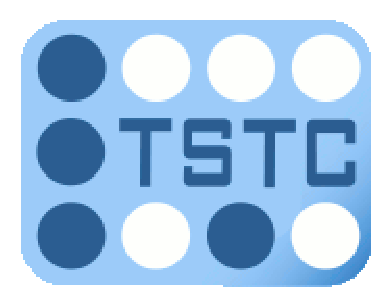
\includegraphics[width=0.15\textwidth]{imagenes/tstc}\\[0.1cm]
\textsc{Departamento de Teoría de la Señal, Telemática y Comunicaciones}\\
\textsc{---}\\
Granada, Julio de 2015
\end{minipage}
\addtolength{\textwidth}{\centeroffset}
\vspace{\stretch{2}}

 
\end{titlepage}






\cleardoublepage
\thispagestyle{empty}

\begin{center}
{\large\bfseries Diseño y evaluación de un servicio OpenFlow de provisión de Calidad de Experiencia sobre Mininet}\\
\end{center}
\begin{center}
Cristian Alfonso Prieto Sánchez\\
\end{center}

%\vspace{0.7cm}
\noindent{\textbf{Palabras clave}: OpenDayLight, SDN, OpenFlow, Routing, Dijkstra, redes, Java, Controller, mininet, QoE, QoS.}\\

\vspace{0.7cm}
\noindent{\textbf{Resumen}}\\

Las redes definidas por software (\ac{SDN}) presentan un cambio de paradigma para las redes futuras, consistente en la separación del plano de control y el de transporte. Introducen grandes ventajas frente a las redes tradicionales. Por un lado los elementos de red podrán ser mucho más sencillos, sin que esto suponga pérdidas de capacidad en ningún caso. Por otro lado se conseguirá un aumento en flexibilidad y velocidad en la automatización de tareas de red debido a la centralización de estas tareas en un elemento único, el controlador.

Las grandes ventajas que presenta este nuevo paradigma ha atraído la atención de grandes fabricantes de la industria, que ya cuenten con sus propias soluciones para redes \ac{SDN}. Esto no ha supuesto una privatización de conocimiento o un estancamiento de la tecnología, todo lo contrario, ya que ha impulsado las líneas de investigación sobre redes \ac{SDN} en la comunidad científica e investigadora.

La transmisión de contenido multimedia supone uno de las mayores fuentes de tráfico de red en la actualidad, y se estima que tráficos como el de vídeo constituirán más del 75\% del tráfico de red en menos de 5 años. Estas transmisiones multimedia requerirán unas condiciones mínimas de transmisión para asegurar \ac{QoS}. 

En este trabajado se pretenden desarrollar servicios basados en \ac{SDN} capaces de proporcionar \ac{QoE} para aplicaciones multimedia, demostrando la capacidad de redes programables para satisfacer requisitos. Concretamente, se diseñará y desarrollará un protocolo de encaminamiento basado en QoS para distintos tipos de tráfico, que sea capaz de reaccionar rápidamente en caso de cambios en la topología de red. Para ello estudiaremos los conceptos que permiten la conformación de redes \ac{SDN}, los protocolos de control y gestión desarrollados para esta tecnología y las principales implementaciones y entornos de desarrollo (privadas y abiertas) de controladores \ac{SDN}.

El ahorro en costes es otro de los puntos que ha suscitado el interés de las grandes compañías por redes \ac{SDN}. La solución presentada en este trabajo también aborda este aspecto, ya que automatiza la configuración de red, permitiendo al administrador ahorrar costes y tiempo en tareas de gestión de redes.  

Para poder llevar a cabo la implementación de la solución propuesta, será asimismo necesario familiarizarse con el uso de varias herramientas de desarrollo de aplicaciones de red SDN (emulador de redes, entornos de desarrollo, etc) que permitan alcanzar los objetivos propuestos. 

No se pretende dar una solución que abarque todos los conceptos y aspectos relacionados con calidad de servicio y de experiencia, pero sí demostrar que las nuevas redes programables añaden nuevas posibilidades y características que mejoran la gestión y automatización de red.

\cleardoublepage


\thispagestyle{empty}


\begin{center}
{\large\bfseries Diseño y evaluación de un servicio OpenFlow de provisión de Calidad de Experiencia sobre Mininet}\\
\end{center}
\begin{center}
Cristian Alfonso Prieto Sánchez\\
\end{center}

%\vspace{0.7cm}
\noindent{\textbf{Keywords}: OpenDayLight, SDN, OpenFlow, Routing, Dijkstra, redes, Java, Controller, mininet, QoE, QoS.}\\

\vspace{0.7cm}
\noindent{\textbf{Abstract}}\\

The evolution of multimedia services cause new challenges for the service providers. How can they deal with this challenges? In the same direction mobile networks are 5G are evolving and developing new concepts for their network architecture.
At the same time, service providers are looking for new methods to reduce costs of the monitoring and management of their networks.
The SDN architecture is the answer for these questions for many reasons. If we focus on theoretical reasons, SDN allows to reduce \ac{CAPEX} and \ac{OPEX} costs and also allows dynamic and faster management of the network than traditional architectures.
To use the new architectures will be necessary a special design protocol which allows to manage the new networks. A lot of different protocols could be used, but the most important is OpenFlow protocol. OpenFlow is specially designed to get the best capacity of the new network architecture SDN so that is the principal reason to use this protocol. Additionally, other reasons to select OpenFlow is that it has open source implementations, and that it is supported by a number of important companies.

The support for the OpenFlow protocol will be very important to decide which controller we will choose for our solution. OpenDayLight is a new controller under the Linux Foundation which is supported for a lot of companies such as Cisco, Intel or HP among others. Also, it is necessary to put the focus on the open character of the project, and the active support given by the community of users.

OpenDayLight satisfies these necessary requisites. It is an Open Source controller with  enough facilities to develop a network aplication for the controller. Throughout the project, we will study the concepts which make possible the development of new network applications in an SDN controller.

In this project we will focus on the \ac{QoE} and \ac{QoS} support that SDN networks can provide to developers. We will design a solution to fullfill this objetive. After this we will evaluate our proposal. The solution will use traffic engineering to evaluate the costs for each link (edge). It will  also use the Dijkstra Algorithm to find the best path between two nodes. Finally, our solution will provide a way to delete the routes in switches if a broke path is detected  (for example, a down link) so we will develope a solution for guaranteeing that the network will work after links outages.

Finally we will implement the solution using the JAVA programming language. We will describe the necessary steps to get a robust aplication which should work correctly.

We will evaluate the developed application by network emulation, defining several experimental scenarios.  The evaluation tests will consider many differents points of view to be sure about the correct work under distinct working conditions. We will use different measures to estimate the subjective assessment of final users under different situations. These estimations will be obtained by applying different standardized theoretical models which will be studied along the document.

To end with, we will present the conclusions about this project in the last chapter, as well as the keys to continue studing and developing in future works.


\chapter*{}
\thispagestyle{empty}

\noindent\rule[-1ex]{\textwidth}{2pt}\\[4.5ex]

Yo, \textbf{Cristian Alfonso Prieto Sánchez}, alumno de la titulación Grado en Ingeniería de Tecnologías de Telecomunicación de la \textbf{Escuela Técnica Superior
de Ingenierías Informática y de Telecomunicación de la Universidad de Granada}, con DNI 75926381-T, autorizo la
ubicación de la siguiente copia de mi Trabajo Fin de Grado en la biblioteca del centro para que pueda ser
consultada por las personas que lo deseen.

\vspace{6cm}

\noindent Fdo: Cristian Alfonso Prieto Sánchez

\vspace{2cm}

\begin{flushright}
Granada a 6 de Julio de 2015.
\end{flushright}


\chapter*{}
\thispagestyle{empty}

\noindent\rule[-1ex]{\textwidth}{2pt}\\[4.5ex]

D. \textbf{Juan José Ramos Muñoz}, Profesor del Área de Telemática del Departamento Teoría de la Señal, Telemática y Comunicaciones de la Universidad de Granada.

\vspace{0.5cm}


\vspace{0.5cm}

\textbf{Informa:}

\vspace{0.5cm}

Que el presente trabajo, titulado \textit{\textbf{Diseño y evaluación de un servicio OpenFlow de provisión de Calidad de Experiencia sobre Mininet}},
ha sido realizado bajo su supervisión por \textbf{Cristian Alfonso Prieto Sánchez}, y autorizo la defensa de dicho trabajo ante el tribunal
que corresponda.

\vspace{0.5cm}

Y para que conste, expiden y firman el presente informe en Granada a 6 de Julio de 2015.

\vspace{1cm}

\textbf{El director:}

\vspace{5cm}

\noindent \textbf{Juan José Ramos Muñoz}

\chapter*{Agradecimientos}
\thispagestyle{empty}

       \vspace{1cm}


\begin{flushright}
\textit{Dedicado a \\
Cada persona que me ha apoyado. \\
Que siempre me han hecho creer en mí. \\
Que nunca han dejado que me rinda.\\
Como no a Manu, el apoyo de todos estos meses\\
y en especial a ella que siempre está \\
y siempre saca lo mejor de mí.}
\end{flushright}



\pagenumbering{Roman}

\cleardoublepage
\phantomsection
\addcontentsline{toc}{chapter}{Referencia de siglas y acrónimos}

\begin{huge}
\textbf{Referencia de siglas y acrónimos}
\end{huge}

\begin{acronym}
\acro{AAA}{Authentication, Authorization and Accounting}
\acro{AD}{API Driven}
\acro{API}{Application Programming Interface}
\acro{APIC}{Application Policy Infrastructure Controller}
\acro{ATM}{Asynchronous Transfer Mode}
\acro{BGP}{Border Gateway Protocol}
\acro{CAPEX}{CAPital EXpenditures}
\acro{DHCP}{Dinamic Host Control Protocol}
\acro{DOM}{Document Object Model}
\acro{ForCES}{Forwarding and Control Element Separation}
\acro{GENI}{Global Environment for Network Innovations}
\acro{HD}{High Definition}
\acro{HTML}{HyperText Markup Language}
\acro{HTTP}{HyperText Transfer Protocol}
\acro{ICMP}{Internet Control Message Protocol}
\acro{IDE}{Integrated Development Environment}
\acro{IETF}{Internet Engineering Task Force}
\acro{IP}{Internet Protocol}
\acro{IRIS}{Interconexión de Recursos InformáticoS}
\acro{ITU}{Unión Internacional de telecomunicaciones}
\acro{JAR}{Java ARchive}
\acro{JSON}{JavaScript Object Notation}
\acro{MD}{Model Driven}
\acro{MOS}{Mean Opinion Score}
\acro{MPEG}{Moving Picture Experts Group}
\acro{MPLS}{MultiProtocol Label Switching}
\acro{NAT}{Network Address Traslation}
\acro{NB}{NorthBound}
\acro{NETCONF}{Network Configuration Protocol}
\acro{ODL}{OpenDayLight}
\acro{ONF}{Open Networking Foundation}
\acro{ONS}{Open Networking Summit}
\acro{OPEX}{OPEratix EXpense}
\acro{OSGi}{Open Services Gateway Initiative}
\acro{OSPF}{Open Shortest Path First}
\acro{PASITO}{Plataforma de Análisis de Servicios de Telecomunicaciones}
\acro{PCE}{Path Computation Element}
\acro{PCEP}{Path Computation Element Protocol}
\acro{POM}{Project Object Model}
\acro{QoE}{Calidad de Experiencia}
\acro{QoS}{Calidad de Servicio}
\acro{RCP}{Routing Control Platform}
\acro{REST}{Representational State Transfer}
\acro{RTP}{Real-time Routing Protocol}
\acro{SAL}{Service Abstraction Layer}
\acro{SB}{SouthBound}
\acro{SDN}{Software Defined Networking}
\acro{SO}{Sistema Operativo}
\acro{SNMP}{Simple Network Management Protocol}
\acro{TCP}{Transmission Control Protocol}
\acro{TLS}{Transport Layer Security}
\acro{TTL}{Time To Life}
\acro{UC}{Unified Communications}
\acro{UDP}{Usser Datagram Protocol}
\acro{UML}{Unified Modeling Language}
\acro{VLC}{Video Local Area Network Client}
\acro{VAN}{Virtual Application Networks}
\acro{VoIP}{Voice Over IP}
\acro{VOIP}{Voice Over IP}
\acro{XML}{eXtensible Markup Language}

\end{acronym}

\newpage

\thispagestyle{empty}

%\pagenumbering{Roman}
\tableofcontents % indice de contenidos

\cleardoublepage
\addcontentsline{toc}{chapter}{Índice de figuras} % para que aparezca en el indice de contenidos
\listoffigures % indice de figuras

\cleardoublepage
\renewcommand{\listtablename}{Índice de tablas}
\renewcommand{\tablename}{Tabla}
\addcontentsline{toc}{chapter}{Índice de tablas} % para que aparezca en el indice de contenidos
\listoftables % indice de tablas

\chapter{Introducción y objetivos}\label{cap.introduccion}
\pagenumbering{arabic} % para empezar la numeración con números
Este primer capítulo se presentarán los conceptos básicos que se trabajarán a lo largo de esta memoria. En primer lugar se describirá el marco global donde se encuadra \ac{SDN} (\emph{Software Defined Networking}). Una vez presentada el área de aplicación del objeto de estudio de este trabajo, se presentarán las motivaciones que justifican la realización de este proyecto, y los objetivos que se pretenden alcanzar. Por último se describirá brevemente la estructura de la memoria para ayudar al lector a localizar con claridad los capítulos mayor interés.

\section{Contexto}\label{contexto}
Si nos detenemos en la evolución futura de redes móviles nos topamos con las novedosas redes 5G. Redes que prometen una mayor capacidad y mejores capacidades para ofrecer servicios. Para alcanzar estas capacidades los proveedores de servicios necesitan adoptar nuevas arquitecturas de red, y \ac{SDN} surge como una de las de mayor peso.

Estos proveedores buscan una constante evolución en sus redes, enfocada a conseguir mayor flexibilidad y mejoras de servicio sin aumentar costes, o incluso reduciéndolos. Existen dos tipos de costes asociados a las redes: el \ac{CAPEX} (\emph{CAPital Expenditure}) y el \ac{OPEX} (\emph{OPerational Expenditure}). En la sección \ref{SDN} se realiza un estudio sobre como \ac{SDN} puede ser el motor impulsor de las nuevas arquitecturas de red, como además se demuestra su aplicación en \cite{googleOpenFlow} entre otras que se estudiarán en los siguientes apartados.

Otro de los aspectos fundamentales en el impulso de redes \ac{SDN} es el crecimiento de dispositivos con necesidades de acceso a la red. Este crecimiento está sustentado en dos pilares: desarrollo de zonas sin acceso e implantación de sistemas \textit{wearables}. Teniendo en cuenta estos dos focos de crecimiento, según \textit{Cisco} se puede estimar un crecimiento en el tráfico de red como el presentado en la figura \ref{IP_Traffic_2013-2018} extraído de \cite{cisco2014cisco}\nocite{cisco2014cisco}.

\begin{figure}[tb]
\begin{center}
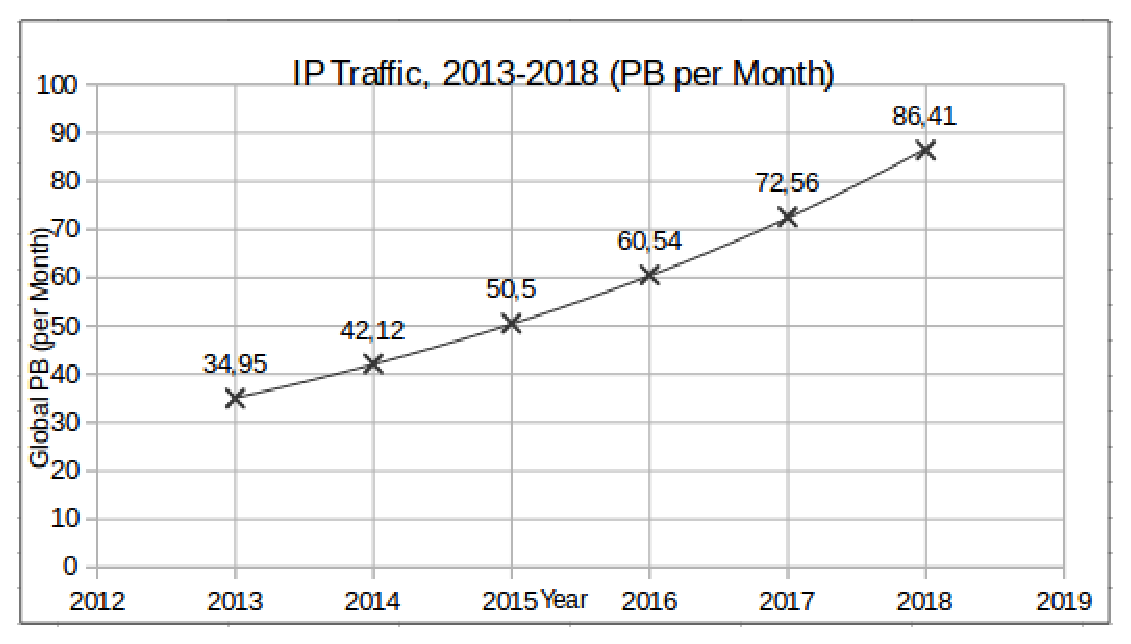
\includegraphics[scale=0.7]{./figuras/IPTraffic1}
\caption[IP Traffic, 2013-2018 (PetaBytes por mes).] {IP Traffic, 2013-2018 (PetaBytes por mes). Datos tomados de \cite{cisco2014cisco}.}
\label{IP_Traffic_2013-2018}
\end{center}
\end{figure}

De esta figura podemos ver como el crecimiento de usuarios y tráfico seguirá una tendencia exponencial, con un crecimiento anual del 21\%, siendo todo un reto para la industria soportar tal cantidad de tráfico. Si ahora desglosamos el crecimiento por tipo de tráfico obtenemos los resultados que se aprecian en la figura \ref{IP_Traffic_2013-2018_2}. Podemos comprobar que el mayor crecimiento es el de tráfico en redes móviles (crecimiento en porcentaje, no en volumen), con un crecimiento de más del 60\% como se muestra en \cite{cisco2014cisco}.

\begin{figure}[htb]
\begin{center}
\hspace*{-0.3cm}
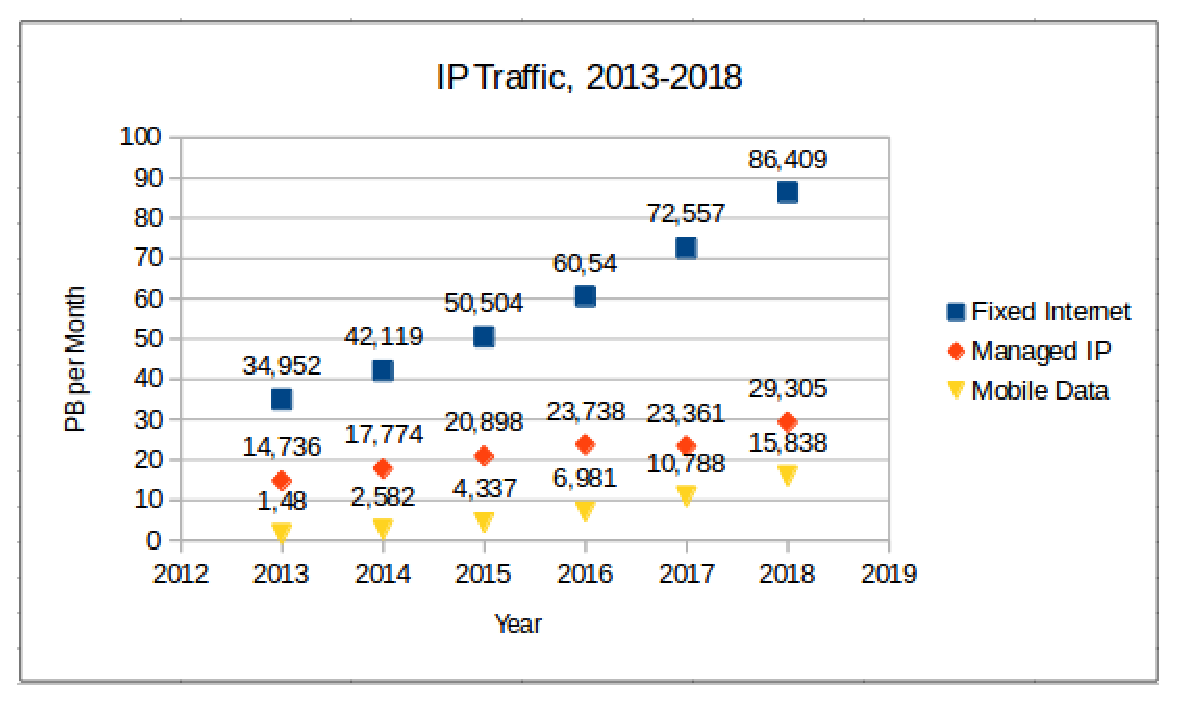
\includegraphics[scale=0.7]{./figuras/IPTraffic2}
\caption[IP Traffic, 2013-2018 (PetaBytes por mes) por tipo de tráfico]{IP Traffic, 2013-2018 (PetaBytes por mes) por tipo de tráfico. Datos tomados de \cite{cisco2014cisco}.}
\label{IP_Traffic_2013-2018_2}
\end{center}
\end{figure}

A partir de estas figuras surgen varias cuestiones ¿Qué tipo de tráfico será el que sufra un mayor aumento y sea más crítico? ¿Están las redes preparadas para soportar un incremento de más del 60\% en redes móviles? En caso de que no lo estuviesen, ¿qué soluciones existen?

Conviene estacar que del tráfico generado por usuarios individuales (más del 80\% del total), uno de los mercados que experimentará mayor crecimiento será el de vídeo por Internet como se indica en la figura \ref{IP_Traffic_2013-2018_video}, demostrando la necesidad de replantear las soluciones actuales para servicios multimedia.

\begin{figure}[htb]
\begin{center}
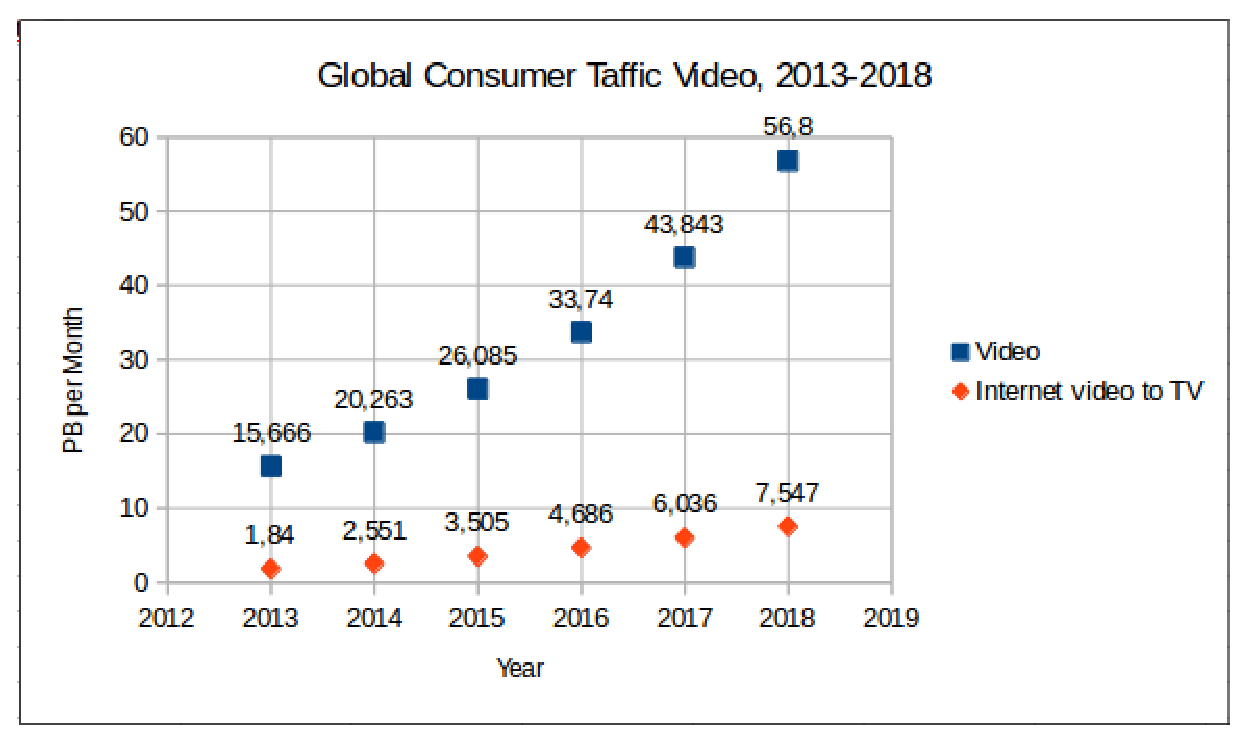
\includegraphics[scale=0.6]{./figuras/IPTraffic4}
\caption[Global Consumer Video Traffic, 2013-2018]{Global Consumer Video Traffic, 2013-2018. Datos tomados de \cite{cisco2014cisco}.}
\label{IP_Traffic_2013-2018_video}
\end{center}
\end{figure}

También es muy interesante para el estudio del contexto el artículo \cite{indexglobal}\nocite{indexglobal} que trata el crecimiento de tráfico en redes móviles, ya que son las que presentan un mayor aumento (aunque repetimos que no en volumen). En este segundo estudio (posterior al primero) se ajusta la previsión para el crecimiento de tráfico para este tipo de redes como se puede comprobar en la figura \ref{IP_Traffic_2014-2019}, pero en líneas generales se puede ver como la tendencia al alza se mantiene.

\begin{figure}[htb]
\begin{center}
\hspace*{-0.3cm}
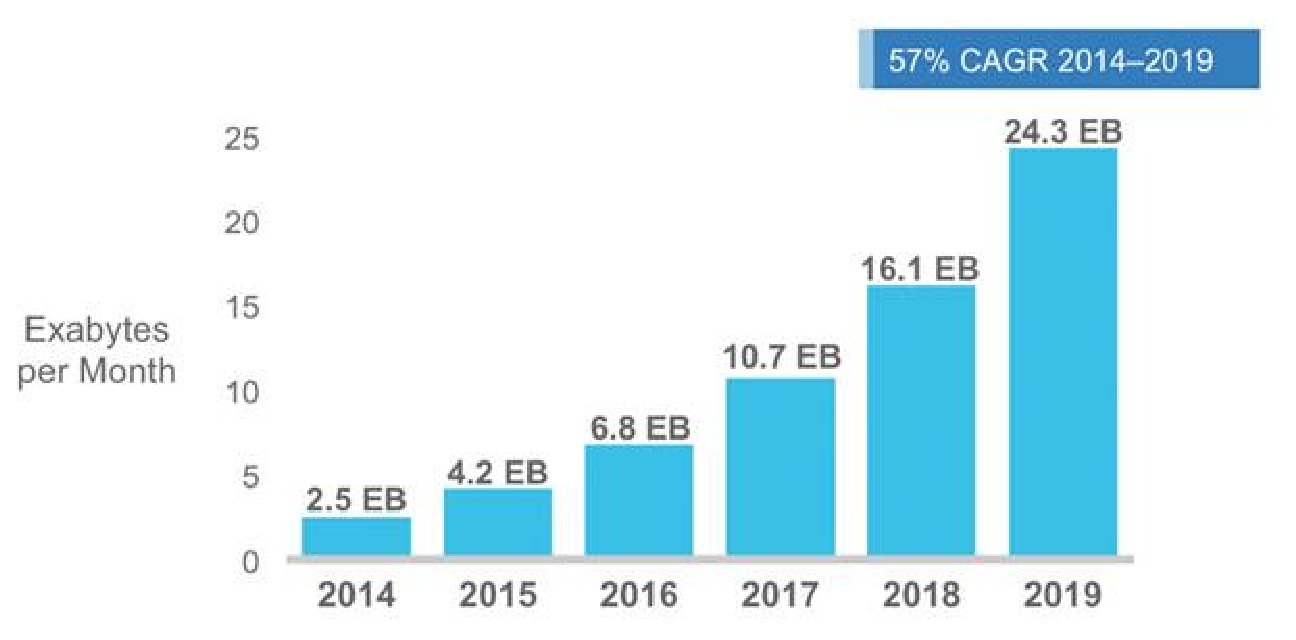
\includegraphics[scale=0.6]{./figuras/IPTraffic3}
\caption[Mobile Data Traffic, 2014-2019 (ExaByte por mes)]{Mobile Data Traffic, 2014-2019 (ExaByte por mes). Imagen tomada de \cite{indexglobal}.}
\label{IP_Traffic_2014-2019}
\end{center}
\end{figure}

Uno de los resultados más interesantes y con mayor relevancia para constatar la importancia de redes \ac{SDN} es la previsión de \cite{indexglobal} sobre a los tipos de tráfico que generaran las redes móviles hasta 2019 como se muestra en la figura \ref{IP_Traffic_2014-2019_types}. 

\begin{figure}[htb]
\begin{center}
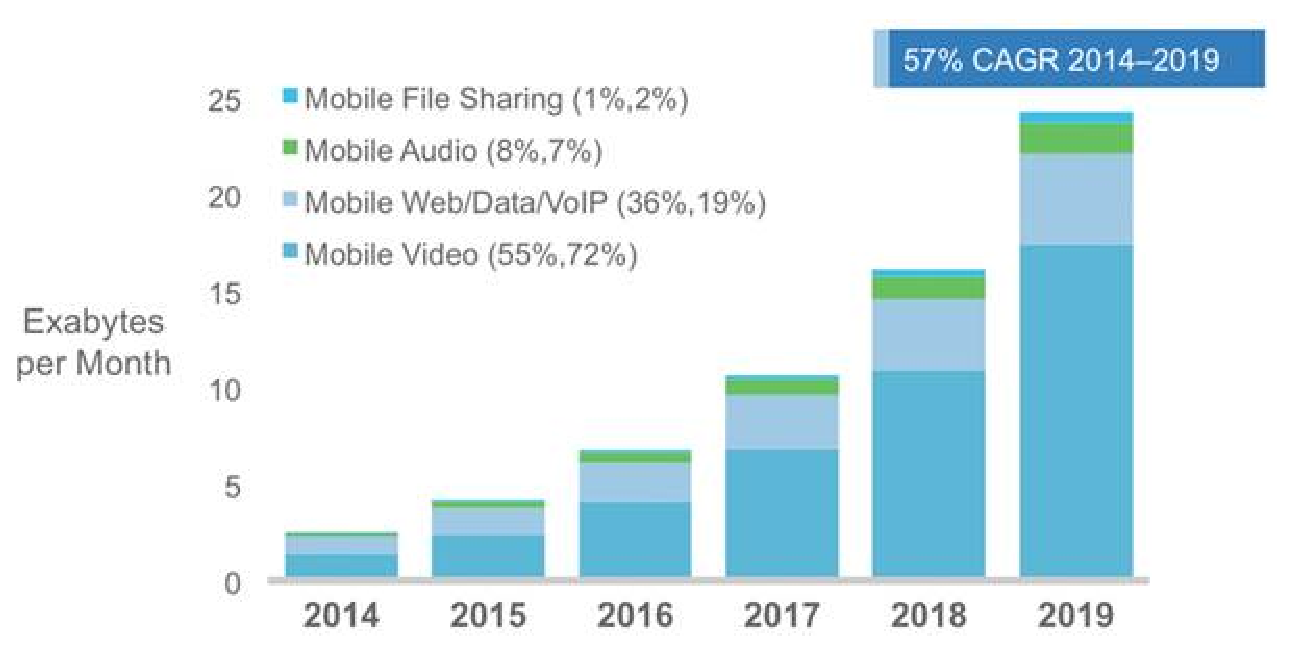
\includegraphics[scale=0.6]{./figuras/IPTraffic6}
\caption[Generación de tráfico por tipos en redes móviles]{Generación de tráfico por tipos en redes móviles. Imagen tomada de \cite{indexglobal}.}
\label{IP_Traffic_2014-2019_types}
\end{center}
\end{figure}

Estos resultados (junto al resto que se recogen en los citados artículos) presentan un contexto idóneo para pensar en la necesidad de evolución de las redes actuales, siendo \ac{SDN} una de las soluciones de mayor relevancia a día de hoy. Se tratará más detenidamente las ventajas de usar \ac{SDN} en la sección \ref{SDN} pero conviene destacar que el éxito de esta tecnología está impulsado por beneficios teórico técnicos (poca inversión inicial, ahorro en costes, agilidad de red) y por casos de éxito real que demuestran las previsiones teóricas (Google\cite{googleOpenFlow}) o casos más concretos para redes multimedia (Verizon\cite{verizonSDN}).

Como último punto en el que situar este proyecto nos hacemos eco de una noticia del 9 de Junio de 2015 (se incluye por su relevancia para la justificación de la elección de \ac{SDN} y la plataforma \emph{OpenDayLight}). Esta noticia trata sobre la forma en la que una gran compañía como es Orange está haciendo uso de \emph{OpenDayLight}. La noticia puede ser consultada en \cite{orangeSDN} y recoge los grandes beneficios que serán presentados en las secciones posteriores. 

%%%%%%%%%%%%%%%%%%%
%
\section{Motivación y objetivos}
La justificación para la realización de este trabajo puede ser sacada directamente del contexto. Por un lado la necesidad de responder ante las demandas de tráfico de manera flexible y rápida, mejorando la gestión de estas redes y automatizándolas. Por otro lado la demanda de contenidos multimedia que precisan de unos fuertes requisitos (vídeo o \ac{VoIP} precisan de un alto ancho de banda o latencias bajas) llevan a las grandes corporaciones del sector a buscar nuevas fórmulas y modelos que permitan satisfacer las demandas requeridas para ofrecer \emph{calidad de servicio} (\emph{QoS, Quality of Service}) que al final se convierte en una buena \emph{calidad de experiencia} (\emph{Quality of Experience, QoE}), es decir, la calidad que percibe el usuario final. Estos dos concetos se pueden definir de la siguiente manera:

\begin{itemize}
\item[•] \textbf{\ac{QoS}.} Definimos \ac{QoS} como el rendimiento promedio de una red telemática. Cuantitativamente mide la calidad de los servicios en base a varios aspectos del servicio de red, tales como tasas de errores, ancho de banda, rendimiento, etc.
\item[•] \textbf{\ac{QoE}.} Cuando se trata el término \ac{QoE} se hace referencia a la calidad subjetiva que es percibida por un usuario final al disfrutar de un servicio ofrecido sobre una red telemática. Es una medida que se ve afectada por todos los elementos de la red extremo a extremo, que repercuten en la percepción final por parte del usuario.
\end{itemize}

Siendo \ac{SDN} una de las soluciones con mayor prestigio y aceptación por parte de la industria, y estando aún en desarrollo continuo, se pretende en este trabajado alcanzar los siguientes objetivos:

\begin{itemize}
\item[•] Revisar el estado de la técnica sobre redes \ac{SDN}, protocolo \emph{OpenFlow} y principales controladores.
\item[•] Revisar el estado de la técnica sobre emulación de redes SDN, \emph{Mininet}.
\item[•] Diseñar una solución capaz de proveer \ac{QoE} en redes \ac{SDN}.
\item[•] Implementar y evaluar dicha solución.
\end{itemize}

\subsection{Alcance del proyecto}
Se describe a continuación el alcance del proyecto. Este proyecto pretende ser un primer paso hacia el estudio de redes \ac{SDN} y sus posibilidades mediante los siguientes puntos:
\begin{itemize}
\item[•] Revisión del estado del arte. Se realizará un amplio estudio sobre las tecnologías implicadas y que son objeto de análisis en este proyecto.
\item[•] Estudio de herramientas \ac{SDN}. Será necesario describir las herramientas que posibilitarán la emulación y evaluación de las capacidades de redes \ac{SDN}.
\item[•] Diseño de la solución. Para alcanzar los objetivos propuestos es necesario el diseño de un algoritmo capaz de integrar las capacidades requeridas. Mediante la división en módulos se pretende encontrar una solución óptima para alcanzar los objetivos propuesto.
\item[•] Implementación de la solución. Para alcanzar los objetivos será necesario encontrar el modo de poder desarrollar e implementar una aplicación en un controlador para redes \ac{SDN}. 
\item[•] Evaluación de la solución. Una vez implementada la solución, se deberá buscar el mejor camino para evaluar ésta.
\end{itemize}

\section{Bibliografía relevante}
Esta sección pretende recoger las citas bibliográficas que se han considerado más importantes para la realización del proyecto.

\begin{itemize}
\item[•] \textbf{Redes \ac{SDN}}
Las referencias más destacadas son:

Definición \ac{SDN}: 

\cite{boucadair2014software} M. Boucadair and C. Jacquenet, ``Software-defined networking: A perspective from within
a service provider environment,” 2014.

Historia redes \ac{SDN}: 

\cite{feamster2013road}  N. Feamster, J. Rexford, and E. Zegura, ``The road to sdn,” \textit{Queue}, vol. 11, no. 12, p. 20, 2013.


\item[•] \textbf{\emph{OpenDayLight}}

Guía del desarrollador: 

\cite{developerGuide}  L. Foundation. (2015) Opendaylight developer guide. Último acceso 20 de Junio de 2015. [Online]. Available: \url{https://www.opendaylight.org/sites/opendaylight/files/Developer-Guide-Helium-SR2.pdf}

\item[•] \textbf{Obtención objetiva de calidad de audio sobre \ac{RTP}}

Recomendación ITU: 

\cite{g107}  ITU, ``El modelo e: un modelo informático para utilización en planificación de transmisión",
2014. [Online]. Available: \url{https://www.itu.int/rec/T-REC-G.107-201402-I/es}

\item[•] \textbf{Obtención objetiva de calidad de vídeo sobre \ac{RTP}}

Recomendación ITU: 

\cite{g1070}  ITU, ``Opinion model for video-telephony applications,” 2012. [Online]. Available: \url{http://
www.itu.int/rec/T-REC-G.1070-201207-I/en}


\end{itemize}

\section{Estructura de la memoria}
En esta sección pretendemos presentar la estructura que tendrá la memoria, a fin de que esta sea lo más clara posible, facilitando al lector examinar la memoria de forma organizada y clara.

\begin{itemize}
\item[•] Segundo Capítulo. Comenzaremos realizando un estudio sobre el estado del arte. Se describirán en él las tecnologías y conceptos en los que nos apoyaremos durante el desarrollo teórico/práctico del trabajo, haciendo especial hincapié en la razones que justifican el uso de tecnologías frente a otras.

\item[•] Tercer capítulo. En este capítulo se realiza una planificación temporal y una estimación de costes de toda la realización del trabajo.

\item[•] Cuarto capítulo. Introduciremos el entorno de desarrollo en el que se va a ejecutar todo el proyecto. Siendo este un capítulo de especial importancia para todo aquel que desee replicar o realizar otro proyecto de implementación sobre \ac{SDN}. Trataremos todas las herramientas software que permitirán realizar las pruebas, así como algunos equivalentes en el mercado Hardware.

\item[•] Quinto capítulo. En el capítulo quinto nos centraremos en el diseño del sistema, describiendo los ``módulos" que componen la solución propuesta de forma separada, con el fin de esclarecer cada uno de los diseños realizados, como por ejemplo la detección de cambios en la topología.

\item[•] Sexto capítulo. Describiremos la implementación que se ha llevado a cabo a partir del diseño del capítulo \ref{design}, prestando especial atención a aquellas partes de implementación que pueden resultar confusas, como el formato necesario para el código fuente.

\item[•] Séptimo capítulo. Se realizará una evaluación sobre la implementación del sistema. Por un lado evaluaremos las capacidades de los módulos por separado (asegurando el correcto funcionamiento de estos), y posteriormente realizaremos la evaluación del sistema final. Esta evaluación estará dividida en dos, evaluación objetiva (basada en datos como latencia o pérdidas de paquetes) y evaluación subjetiva (experiencia de usuario).

\item[•] Capítulo octavo. Por último en el capítulo séptimo se mostrarán las conclusiones extraídas tras el montaje y evaluación del sistema, así como se intentarán dar las claves que permitan continuar, mejorar o derivar en otras líneas de trabajo futuras.
\end{itemize}

Finalmente se pueden encontrar todas las referencias bibliográficas utilizadas tanto en la realización del proyecto, como las usadas para la realización de la memoria en particular además de un apéndice donde se aporta ayuda con las configuraciones de los diferentes elementos Software, además de código usado en el proyecto y algunos aspectos de configuración.

Como valor añadido a la memoria se incluye el enlace al blog: \url{www.aprendiendoodl.wordpress.com}. Este blog ha sido desarrollado por Manuel Sánchez López y por el autor de esta memoria, Cristian Alfonso Prieto Sánchez, con el objetivo de introducir al mundo \ac{SDN} y \ac{ODL} a todo aquel que esté dando sus primeros pasos con esta tecnología. Consideramos que la guía durante esta iniciación es muy importante debido a la falta de información concreta o falta de tutoriales (tecnología muy novedosa y en constante desarrollo). Por tanto emplazamos a aquel que a partir de la temática de este trabajo y el de Manuel Sánchez López sobre inspección de paquetes, sienta interés por estas novedosas tecnologías, visite el blog donde hallará ejemplos prácticos y explicaciones menos técnicas y más guiadas.


\chapter{Estudio del estado del arte}\label{estado.arte}

En este capítulo vamos a describir exhaustivamente las tecnologías en las cuales está basado este trabajo. Comenzaremos con un análisis sobre redes \ac{SDN}. En el siguiente punto analizaremos el protocolo más importante para redes \ac{SDN}, \emph{OpenFlow} y algunos otros que han surgido a partir del interés generado. Por último haremos un repaso de los principales controladores de redes \ac{SDN} y centraremos la atención en el elegido para el desarrollo, \emph{OpenDayLight}.

\section{Software Defined Networking}\label{SDN}
Hasta ahora se han presentado los requisitos que deberán cumplir las redes futuras (crecimiento del número de usuarios, redes móviles o transmisión multimedia) y se han establecido los bases por las cuales podemos decir que las redes actuales serán incapaces de satisfacer la demanda de los usuarios, todo ello en la sección \ref{contexto}. El desafío de la industria consiste en idear un nuevo modelo de red capaz de responder a las necesidades futuras, y una de las alternativas más prometedoras son las redes definidas por software, \ac{SDN}.

\subsection{Historia y desarrollo}
Las redes definidas por software representan un concepto relativamente novedoso que aún se encuentra en desarrollo. Sin embargo el concepto en si lleva años madurándose. A continuación se presenta la evolución de las primeras ideas relacionadas con \ac{SDN} hasta ahora, según el orden presentado en \cite{feamster2013road}.

En los años noventa se produjo el surgimiento de Internet para el gran público. El nacimiento de esta revolucionaria tecnología provocó un afán por la mejora de infraestructuras de red. Se pretendía poder gestionarlas de un modo mucho más efectivo, siendo uno de los objetivos hacerlas programables, siendo capaces de conmutar según las necesidades de cada momento.

El despliegue de Internet provocó un enorme desarrollo en las aplicaciones que a su vez se tradujo en la necesidad de diseñar nuevos protocolos de red para poder soportarlas. El problema residía en que cada protocolo debía ser estandarizado por la \emph{\ac{IETF}}, siendo este un proceso demasiado lento para muchos investigadores.

Como alternativa, algunos grupos de investigación apostaron por un enfoque de apertura de control sobre las redes, permitiendo reprogramar las redes. Pero dado que las redes convencionales no eran ni son programables, surgieron las \textit{redes activas}. Esta redes supusieron una aproximación radical hacia el control de red, basándose en una interfaz programable con capacidad para mostrar los recursos de cada nodo individual y capaz de aplicar acciones concretas para un grupo de paquetes definidos (flujos).

En contraposición, se encontraban muchos grupos que apostaban por la simplicidad en el núcleo de red, ya que según ellos esta parte es crítica para el éxito de Internet. Aún así la comunidad de redes activas propuso alternativas a los modelos tradicionales basados en \ac{IP} o \ac{ATM} (alternativas dominantes en la época). Surgieron dos modelos programables.

\begin{itemize}
\item[•] \textbf{Modelo encapsulado.} Se propuso en este modelo encapsular las acciones que debía ejecutar el nodo, dentro de la propia información de cada paquete. De esta manera, porciones de código que se interpretaban en los nodos de red eran transportadas por los propios paquetes.
\item[•] \textbf{Modelo programable.} El código que debía ser ejecutado por cada nodo se generaba por aplicaciones o procesos externos al nodo.
\end{itemize}

El desarrollo \textit{redes activas}, que no llego a extenderse ampliamente, dio lugar a tecnologías que hoy día se recogen y usan en \ac{SDN}, como las funciones programables de los elementos de red, virtualización de red, por ejemplo.

A principios del nuevo milenio surge un nuevo concepto: la separación del plano de control (donde se encuentran las funciones de control de red) y de datos (funciones de reenvío de paquetes). El aumento del tráfico en Internet y la necesidad de redes manejables, predecibles y confiables llevaron a los investigadores a buscar nuevos enfoques para las funciones de gestión de red. Una de estas funciones era la ingeniería de tráfico, cuyas posibilidades se veían limitadas por los protocolos de enrutamiento convencionales, perdiendo capacidad.

La tarea de analizar y resolver problemas de configuración o controlar el comportamiento de enrutamiento de paquetes recaía durante esta época en \textit{switches} y \textit{routers}, una tarea demasiado compleja para los recursos con los que trabajaban. Fue esta razón la que derivó en la separación de estos planos y la que dio lugar a posteriores estándares y soluciones.

El crecimiento de Internet llevó a las empresas de equipos hardware a incluir lógica de reenvío de paquetes en estos equipos (separando así los dos planos). Mientras tanto los proveedores de servicio luchaban por gestionar las redes (crecientes) mientras añadían nuevos servicios para el usuario. En este contexto surgen varias innovaciones que serán importantes para el posterior desarrollo de \ac{SDN}. Por ejemplo surgió una interfaz abierta entre los planos de datos y control, \ac{ForCES}, estandarizada por la \ac{IETF} o NetLink (proporciona la funcionalidad de reenvío de paquetes a nivel de núcleo Línux). Desde el punto de vista del control centralizado surgen \textit{\ac{RCP}}, arquitecturas \textit{SoftRouter} (equipos programables) y el protocolo \textit{\ac{PCE}}. Todos estos conceptos serán clave en el desarrollo futuro de \ac{SDN} como se describe en \cite{feamster2013road}.

En ese momento era necesario encontrar el modo de separar el plano de control y datos como en la imagen \ref{planoControl}. El comienzo de este desarrollo estuvo centrado en la investigación de nuevas arquitecturas que permitieran el control lógico centralizado. Uno de los primeros proyectos (y de los de mayor importancia) fue el proyecto 4D\footnote{http://www.cs.cmu.edu/~4D/}. En este proyecto se establecía la separación de la red en cuatro capas como se explica en \cite{greenberg2005clean}. Las cuatro capas que se contemplaron correspondían al \textit{plano de datos} (encargado del reenvío basándose en las reglas, configurables), \textit{plano de descubrimiento} (encargado de recoger estadísticas de tráfico y equipos en la red), el \textit{plano de diseminación} (encargado de instalar reglas en los equipos que se ocuparán de aplicarlas) y el \textit{plano de decisión} (encargado de tomar decisiones acerca del enrutamiento de paquetes en la red).

\begin{figure}[tb]
\centering
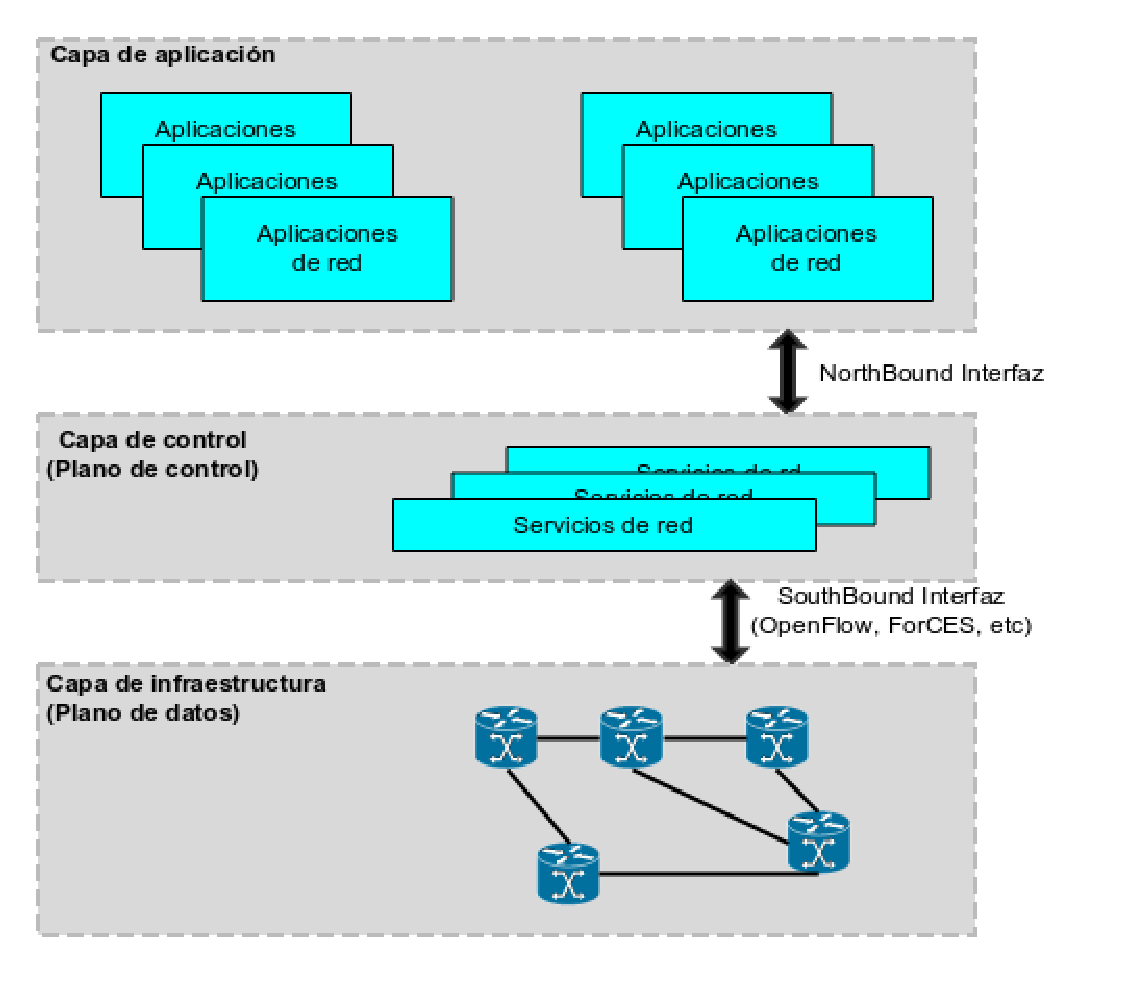
\includegraphics[scale=0.5]{./figuras/planoscontroldatos}
\caption{Arquitectura para la separación de planos de control y datos.}\label{planoControl}
\end{figure}

\label{SDNHistoryOpenflow}
A partir de este trabajo, numerosos grupos comenzaron a seguir esta línea de investigación. El más relevante para nuestro proyecto, y uno de los más importantes, es el proyecto Ethane. Surgido en la universidad de Stanford, y cuyo desarrollo acabó siendo la base de \emph{OpenFlow}. Para más información sobre los objetivos y resultados obtenidos en este proyecto se aconseja visitar \cite{casado2007ethane}.

El desarrollo total de \emph{OpenFlow} como estándar abierto se produjo a mediados de la primera década del actual siglo, gracias a la experimentación en redes de gran escala (PlanetLab\cite{planetlab} o Emulab\cite{emulab} entre otros), que dieron a lugar a un gran entusiasmo por parte de la comunidad investigadora a la hora de realizar experimentos en estos entornos. De este entusiasmo surgió el \textit{Clean Slate Program}\footnote{Programa de investigación de la universidad de Stanford que trabaja en como debería ser rediseñado Internet desde 0 (borrón y cuenta nueva).} enfocado en la investigación sobre redes universitarias y que daría lugar al estándar \emph{OpenFlow} como hoy lo conocemos.

\subsection{Definición SDN}
Para definir \ac{SDN} vamos a recurrir a la propia definición realizada por la \ac{ONF} en \cite{ONFDefinition}\nocite{ONFDefinition}.

\ac{SDN} es una arquitectura dinámica, manejable, rentable y adaptable, capaz de soportar el gran ancho de banda y la naturaleza dinámica de las aplicaciones actuales. Las características más importantes de \ac{SDN} son:

\begin{itemize}
	\item[•] \textbf{Son redes programables.} El desacoplamiento entre las capas de control y aplicación permiten la programación directa de la red sin preocuparnos por las funciones de reenvío.
	\item[•] \textbf{Permite un desarrollo ágil.} De igual manera que permite la programación dinámica de red, el desacoplamiento entre capas también permite que la modificación de flujos y funciones de red sea muy rápido y adaptable.
	\item[•] \textbf{Permite la gestión centralizada.} La arquitectura \ac{SDN} se basa en un control centralizado que mantiene una visión global de la red y que es el elemento que interactúa con todos los demás añadiendo, eliminando o modificando flujos.
	\item[•] \textbf{Permite automatizar la programación de los dispositivos.} \ac{SDN} permite a los administradores configurar programas escritos por ellos mismos (\ac{SDN} no depende de Software propietario) que agilicen todo el proceso de configuración, optimización y administración de recursos de red.
	\item[•] \textbf{Está basada en estándares abiertos.} Cuando \ac{SDN} se implementa a través de estándares abiertos, ésta permite la simplificación de red al no depender de proveedores específicos, dispositivos de traducción o protocolos propietarios.
\end{itemize}

La figura \ref{planoControl} es una simplificación de la arquitectura \ac{SDN} donde podemos comprobar la separación entre capas gracias al uso de protocolos de control gracias al uso de protocolos de control.

\subsubsection{¿Por qué \ac{SDN}?}

Para justificar la relevancia de \ac{SDN} y su uso en este trabajo podemos recurrir a razones principales: la primera, los beneficios de usar \ac{SDN} frente a otras tecnologías o arquitecturas. La segunda, el apoyo por parte de la industria del sector.

\subsubsection{Beneficios teóricos.} 

Dentro de los beneficios de implantar \ac{SDN} frente a otras arquitecturas existentes, encontramos dos visiones: beneficios económicos y beneficios técnicos. 

Dentro de los beneficios económicos destacamos:

\begin{itemize}
\item[•] \textbf{Reducción del \ac{CAPEX}.} Permite la reutilización de hardware existente gracias a las compatibilidades mencionadas y a la \textit{SouthBound} \ac{API}, reduciendo de este modo el gasto inicial en instalación de equipos nuevos.
\item[•] \textbf{Reducción del \ac{OPEX}.} Ahorro en costes operativos debido a la mejora en la gestión que introduce una arquitectura \ac{SDN}. La mejora se ve reflejada en un mejor orden logístico más centralizado, y en ahorro de tiempo de gestión por parte de los administradores.
\end{itemize}

Desde el punto de vista técnico ya se han mencionado algunas de las ventajas de \ac{SDN}, siendo las más importantes las referidas a la agilidad y flexibilidad que se gana usando esta arquitectura. Además las posibilidades futuras de desarrollo están garantizadas gracias al uso de la NorthBound \ac{API} ya que permitirá el desarrollo e innovación en nuevas aplicaciones para \ac{SDN} sin necesidad de cambios en la estructura de la arquitectura.

\subsubsection{Apoyo de la industria.} 

\ac{SDN} cuenta con el apoyo de grandes compañías, que además han conseguido implementar arquitecturas basadas en \ac{SDN} que reducen la complejidad y coste de sus redes cableadas. Existen varios ejemplos, entre ellos el de Google, que ha implementado \emph{OpenFlow} para sus dos redes troncales, obteniendo resultados muy positivos, como se puede comprobar en \cite{googleOpenFlow}\nocite{googleOpenFlow}.

Otros casos de éxito son los de Verizon\cite{verizonSDN}\nocite{verizonSDN} (despliegue de red \ac{SDN} para servicios de vídeo distribuido o el caso de ATT\cite{attSDN}\nocite{attSDN} que tiene un plan para la mejora de su arquitectura a través de virtualización y uso de \ac{SDN}.

Estos son claros ejemplos del desarrollo y funcionalidad de \ac{SDN} que justifican este trabajo. A continuación se describe la arquitectura que hace posible que \ac{SDN} sea tan beneficiosa frente a otras soluciones.

\subsubsection{Arquitectura y elementos en \ac{SDN}.}

En \ac{SDN} todo se basa en el elemento central, el controlador. El controlador será el elemento que comunicará todas las capas mediante el uso de \ac{API}s. Para conseguir la separación de los planos de control y de datos, será necesario el uso de dos \ac{API}s. \textit{Northbound} \ac{API} (que comunica con la capa de aplicación) y \textit{SouthBound} \ac{API} (que comunica con los elementos al sur del controlador).

Para ver con más claridad como interactúan los elementos en \ac{SDN} se incluye la figura \ref{SDNSchematic}, donde se puede comprobar perfectamente como todos los requerimientos de las aplicaciones del plano al norte, pasan por el controlador a través de la \textit{Northbound} \ac{API}, y que todas las instrucciones hacia elementos de red pasan por la \textit{SouthBound} \ac{API} (\ac{SDN} Control-Data-Plane Interface en la imagen). Gracias al uso de la \textit{SouthBound} \ac{API}, el tipo de elemento de red sea indiferente para el controlador y las aplicaciones.

\begin{figure}[tb]
\centering
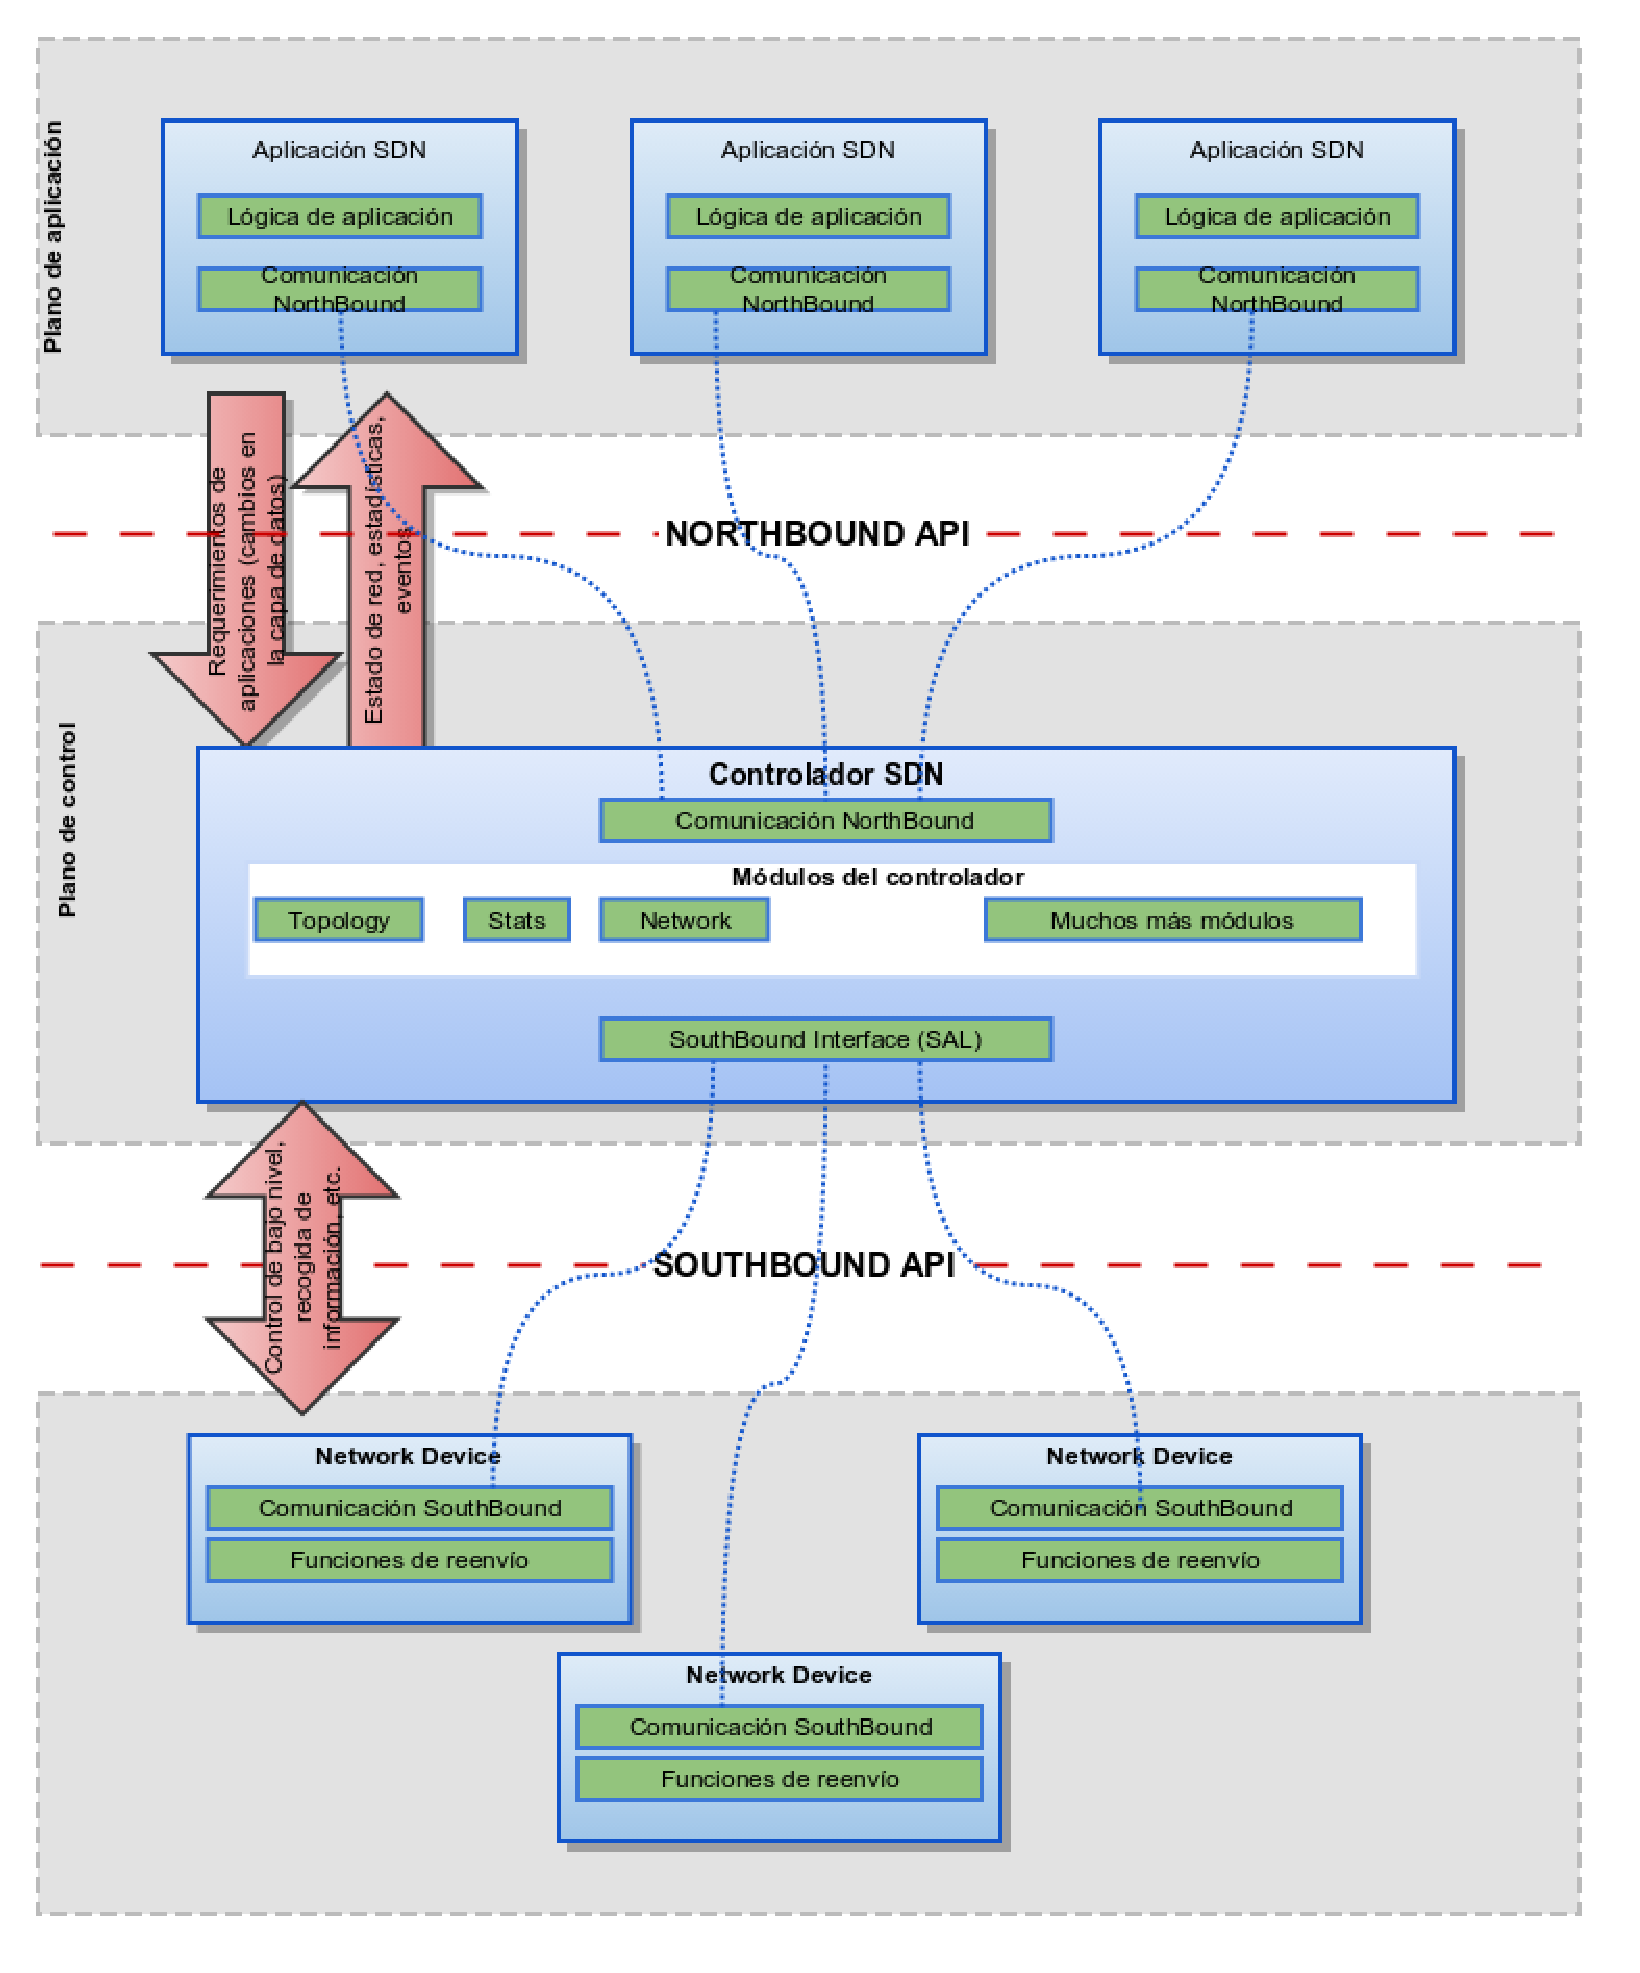
\includegraphics[scale=0.4]{./figuras/SDNSchematic}
\caption[Architecture Overview \ac{SDN}.]{Visión esquemática de la estructura \ac{SDN}. Imagen tomada de \cite{SDN11}} \label{SDNSchematic}
\end{figure}

\begin{itemize}
\item[•]\textbf{Controlador.} Como ya se ha comentado, el controlador \ac{SDN} es el cerebro de la red. Este elemento se encuentra en el centro de todo y se comunica tanto con las aplicaciones (al norte) como con los elementos de transporte (\textit{switches} y \textit{routers}), al sur. Además en algunas soluciones se incluye la posibilidad de definir dominios de controladores \ac{SDN} para hacer las redes \ac{SDN} más escalables y manejables como se indica en \nocite{SDNController}\cite{SDNController}. 

Un controlador \ac{SDN} además estar capacitado para comunicarse a través de las \ac{API}s, suele incluir una serie de módulos que le permiten realizar diferentes tareas de red básicas: inventario de equipos conectados, colección de estadísticas de red u otras funciones. Además los proveedores de soluciones pueden añadir nuevas funciones en el núcleo del controlador según sus necesidades, siendo este uno de los puntos fuertes de la arquitectura \ac{SDN}.

Uno de los controladores más conocidos (y el que se usa en este proyecto) cuenta con los módulos que se muestran en la imagen \ref{ODLFunctionCore}, y que son la base a partir de la cual se pueden construir aplicaciones de red.

\begin{figure}[tb]
	\centering
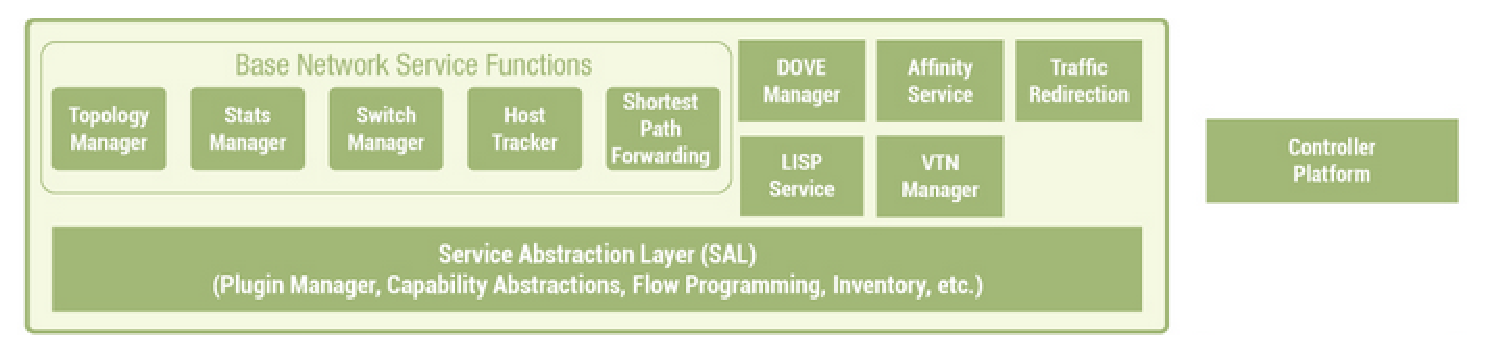
\includegraphics[scale=0.6]{./figuras/ODLFunctionCore}
\caption[Capacidades core \ac{ODL}.]{Capacidades del núcleo de \emph{OpenDayLight}. Imagen extraída de \url{http://www.opendaylight.org/project/technical-overview}.} \label{ODLFunctionCore}
	\end{figure}

\ac{SDN} presenta además la posibilidad de aprovechar protocolos tradicionales de red. En este sentido están trabajando los miembros de uno de los grupos de \ac{IETF} para conseguir que protocolos tradicionales (\ac{OSPF}, \ac{MPLS} o \ac{BGP}, entre otros) sean compatibles con \ac{SDN}. 

Con esto damos por finalizado la parte correspondiente al controlador \ac{SDN}, destacando las posibilidades que ofrece, tanto desde el punto de vista de novedosas funciones, como con la compatibilidad con protocolos antiguos. Las funciones y módulos que incluya un controlador \ac{SDN} serán claves para el desarrollo de aplicaciones, como se comprobará más adelante. 

\item[•] \textbf{\textit{Northbound} y \textit{SouthBound} \ac{API}s.} Son las interfaces que permiten al controlador comunicarse con los elementos al norte y sur de éste.

\textbf{\textit{SouthBound} \ac{API}.} Es la encargada de posibilitar la comunicación del controlador con los elementos de red. Permite hacer cambios dinámicos en los elementos para adecuarse a las necesidades en tiempo real. Además permite la independencia de los elementos subyacentes por parte del controlador, ya que este solo se debe ocupar de enviar instrucciones que esta \ac{API} traduce y transmite al elemento destino al que se dirige la instrucción. Existen varias soluciones para conseguir estas capacidades y la de mayor relevancia por el momento es el ya comentado \emph{OpenFlow}.

\textbf{\textit{Northbound} \ac{API}.} Esta \ac{API} es usada para facilitar la innovación mediante la comunicación del core del controlador con nuevas \ac{API}s. Gracias a la arquitectura \ac{SDN} las nuevas \ac{API}s podrán incluir innovaciones que añadan funciones de red más potentes. Esta \ac{API} es crítica debido al gran número de aplicaciones de diferente procedencia que se soportan a través de ella, pudiendo producirse conflictos o errores entre las aplicaciones si no se respeta el modelo definido en cada caso específico (cada controlador hará uso de diferentes \ac{API}s).

Al ser un componente tan determinante para \ac{SDN}, la \ac{ONF} decidió crear un grupo de trabajado centrado en la \textit{Northbound} \ac{API}, el grupo \textit{NorthBound Working Group}. Este grupo se encarga de escribir código para la \ac{API}, desarrollar prototipos y mostrar claramente las capacidades de dicha \ac{API}.

\end{itemize}

\subsection{Grupos de trabajo \ac{SDN}}
\ac{SDN} es una arquitectura en movimiento y que evoluciona de forma constante. Las mejoras pueden ser de dos tipos: mejoras en la arquitectura o \ac{API} de \ac{SDN} o mejoras en las aplicaciones que posteriormente se comunican con el núcleo \ac{SDN}. Muchos grupos de trabajo están desarrollando e innovando sobre \ac{SDN}, algunos de estos ya han sido citados. Los más destacados son:

\begin{itemize}
\item[•] \textbf{\ac{ONF}.} La \textit{Open Networking Foundation} sigue trabajando en la definición de \ac{SDN} y ha publicado la versión 1.1 de la arquitectura general \ac{SDN}\cite{SDN11}\nocite{SDN11}.
\item[•] \textbf{\textit{\ac{ONF} Wireless and Mobile Working Group.}} Este grupo de trabajo (también de la \ac{ONF}) se creó con la intención de investigar la adaptación de \ac{SDN} y \emph{OpenFlow} para su uso en redes de acceso celular y en transporte inalámbrico. Es un grupo de trabajo orientado a una de las aplicaciones futuras de \ac{SDN}, redes móviles 5G.
\item[•] \textbf{\ac{ONF} \textit{NorthBound Interface Working Group.}} Se ha hecho referencia a este grupo a lo largo de los apartados anteriores. Se encuentra enfocado en la investigación de aplicaciones \ac{SDN}, y el estudio del funcionamiento y uso correcto de la \textit{Northbound} \ac{API}.
\item[•] \textbf{\ac{IETF} \textit{Software Driven Networks}.} Este grupo centra sus esfuerzos en el estudio de \ac{SDN} dentro del marco \ac{IETF}, completando huecos que consideran vacíos de la definición de \ac{SDN} original. Proponen cambios, aportan soluciones y en definitiva estudian \ac{SDN} desde otras perspectivas.
\item[•] \textbf{UC\footnote{Unified Communications}\textit{ Software Defined Networking Activity Group}.} Este grupo de trabajo enfoca sus esfuerzos en proyectos de calidad de servicio y transmisión de datos multimedia sobre \ac{SDN}. Los principales puntos de trabajo e innovación de este grupo son: estudio de casos de aplicación, análisis de capacidades \ac{SDN}, definición de un framework para desarrollo \ac{SDN}, definición de las \ac{API}s necesarias y definición de un programa de certificación \ac{SDN}.
\end{itemize}

Estos son solo una pequeña parte de los grupos que en este momento se encuentran trabajando en la arquitectura \ac{SDN}, quedando patente el interés generado por este nuevo paradigma de red.



\section{\emph{OpenFlow}}\label{openFlow}
Antes de comenzar se debe destacar que \ac{SDN} no es lo mismo que \emph{OpenFlow}. \emph{OpenFlow} es un estándar abierto y que \ac{SDN} puede usar (existen alternativas) para gestionar la red. Lo que si se puede afirmar es que \emph{OpenFlow} se está convirtiendo en el modelo estándar de implementación en redes \ac{SDN}.

De acuerdo a la definición realizada por la \ac{ONF} en \cite{openflowDefinition}, \emph{OpenFlow} es la primera interfaz de comunicaciones definida entre las capas de control y de transporte en una arquitectura \ac{SDN}. Permite el acceso directo y la manipulación de los elementos del plano de control, como \textit{switches} o \textit{routers}. Las tecnologías \ac{SDN} basadas en \emph{OpenFlow} están capacitadas para abordar el gran ancho de banda y la naturaleza dinámica de las aplicaciones actuales, permitiendo adaptar las redes a las necesidades en tiempo real, reduciendo significativamente las operaciones y la complejidad de gestión. En definitiva, \emph{OpenFlow} posibilita casi todo aquello por lo cual las redes \ac{SDN} son tan necesarias en el momento actual.

\subsection{Historia y desarrollo}

Los primeros pasos de OpenFLow están íntimamente ligados a los de \ac{SDN}, como se ha comprobado en la sección referente a la historia de \ac{SDN}, al final de la sección \ref{SDNHistoryOpenflow}. 

El crecimiento de las redes y el éxito de estas, presentó una gran oportunidad de trabajo para los investigadores (mayor importancia en este ámbito), sin embargo en este escenario realizar grandes avances o presentar resultados exitosos se antojaba complicado, ya que no existía ninguna manera práctica de experimentar y probar nuevos desarrollos en un entorno real o lo suficientemente cercano a la realidad para que pudieran considerar como válidos los resultados obtenidos. Como respuesta a esta necesidad surgieron diferentes propuestas. Por ejemplo la red \ac{GENI}\footnote{\url{http://www.geni.net/}}, serguió como una red pensada para facilitar la experimentación en nuevas arquitecturas de red mediante sistemas distribuidos. El concepto de funcionamiento se basaba en las redes programables que, usando virtualización, podían tratar paquetes de experimentos aislados entre sí y de forma simultánea.


\begin{figure}[tb]
\centering
\hspace*{-0.85cm}
\subfigure[Red Geni. Imagen tomada de \url{http://www.geni.net/?page_id=2}]{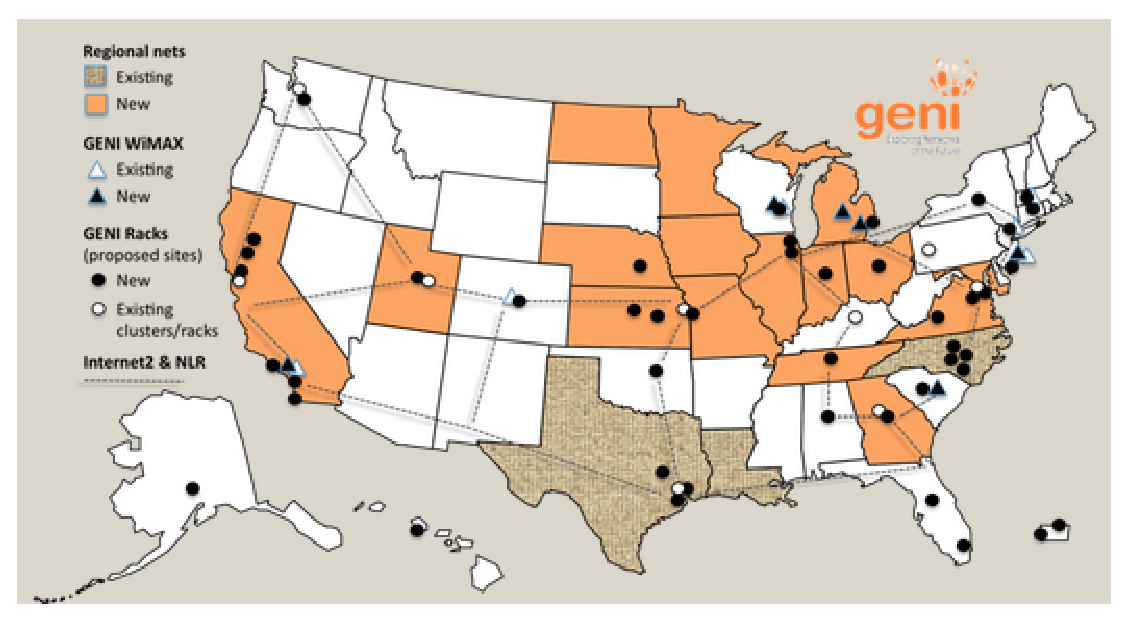
\includegraphics[width=80mm]{./figuras/geni}}
\subfigure[Red PlanetLab. Imagen tomada de \url{https://www.planet-lab.org/}]{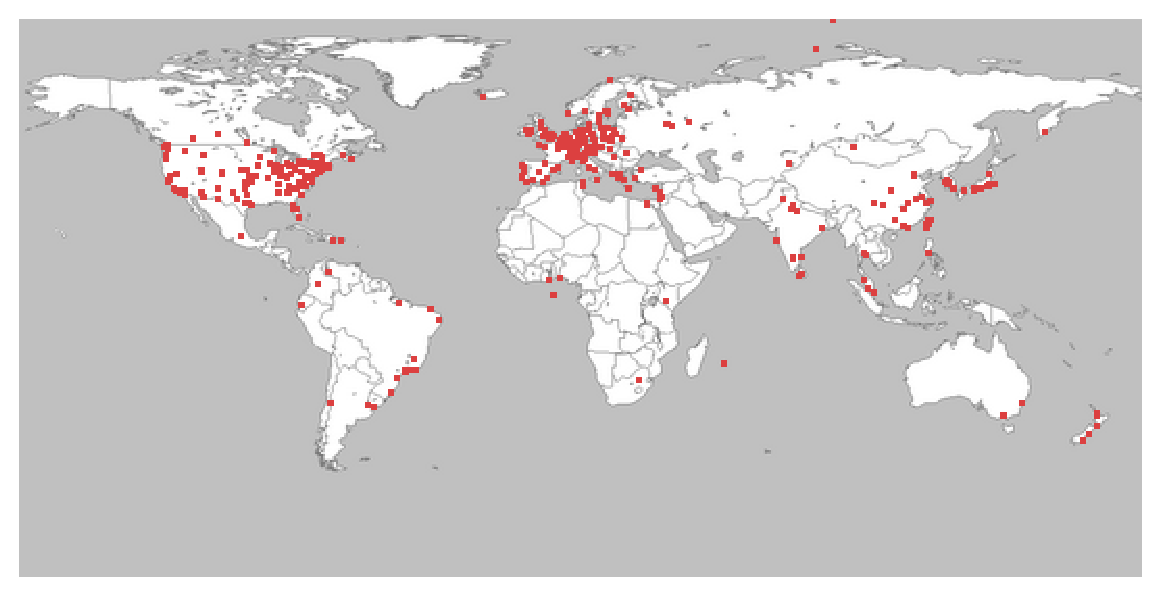
\includegraphics[width=85mm]{./figuras/planetlab}}
\caption{Mapas de redes de experimentación.}
\end{figure}

En España también surgieron redes pensadas para fomentar la innovación mediante la experimentación, como \ac{PASITO}, un proyecto financiado por la secretaría del Estado, gestionado por Red.es y basado en la infraestructura de la \ac{IRIS}, para el desarrollo y la innovación sobre nuevos protocolos de Internet. El esquema de la red \ac{PASITO} puede ser consultado en la figura \ref{iris}.

\begin{figure}[tb]
\centering
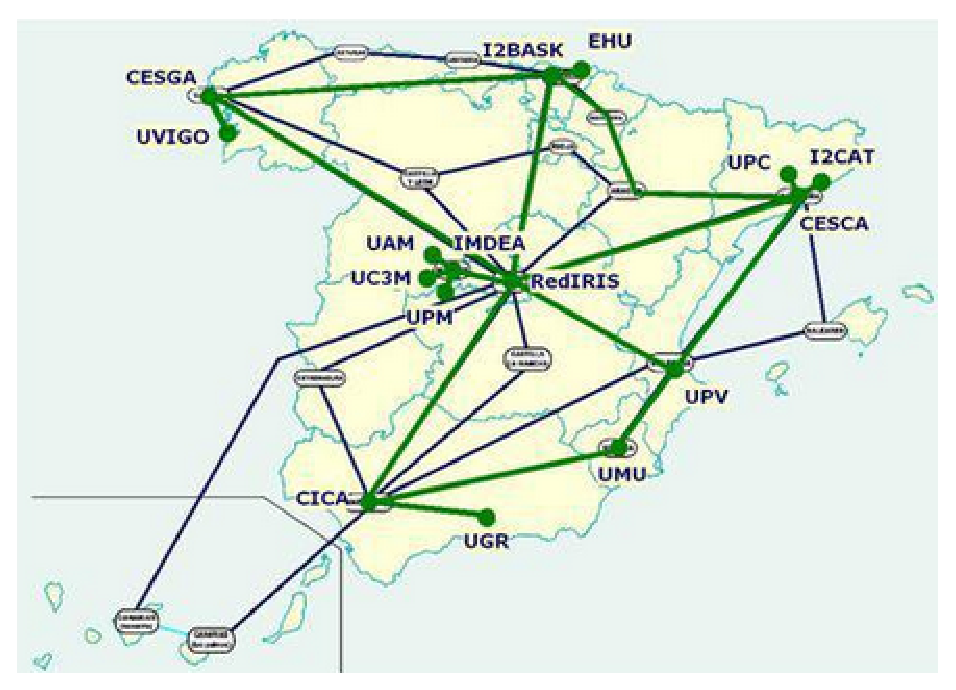
\includegraphics[scale=0.65]{./figuras/iris}
\caption[Mapa de Red PASITO]{Mapa de Red PASITO. Imagen extraída de \url{http://www.rediris.es/jt/jt2006/RedIRIS10.jpg}}\label{iris}
\end{figure}

A partir de estas redes surgieron numerosas posibilidades de desarrollo para la comunidad investigadora. En la universidad de Stanford se creó el Clean Slate Program que acabaría desembocando en el estándar \emph{OpenFlow}. Pronto estas investigaciones llamaron la atención de importantes pesos pesados de la industria. Tanto es así que en la primera versión del estándar \emph{OpenFlow} (versión 1.1, publicada el 28 de Febrero de 2011) estaban incluidos miembros de la talla de Google, Facebook o Microsoft, formando parte de este primer estándar. Posterior al lanzamiento de la primera versión, se hizo público que la \ac{ONF} asumiría la responsabilidad de mantener el estándar a fin de conseguir una estandarización más global y eficaz.

Desde entonces hasta hoy se han ido presentando diferentes versiones del estándar \emph{OpenFlow} \textit{switch} hasta llegar a la más reciente (en Abril de 2015), la versión 1.5.1\footnote{\url{https://www.opennetworking.org/images/stories/downloads/sdn-resources/onf-specifications/openflow/openflow-switch-v1.5.1.pdf}}. Por cuestiones de compatibilidad nosotros usaremos la versión 1.3.0 (versión más reciente soportada por \emph{Mininet}\cite{mininet}).

La gran acogida de \emph{OpenFlow} no sólo se ve reflejada en el continuo proceso de innovación, también podemos contrastarla con el gran número de miembros adheridos a la \ac{ONF}\footnote{\url{https://www.opennetworking.org/our-members}}. En total la \ac{ONF} cuenta con más de 120 miembros, algunos de ellos de la importancia de Cisco, Google, Microsoft, Juniper, Brocade y otros muchos.

\subsection{Alternativas. Redes programables.}

Dentro de las alternativas (y a fin de no extendernos demasiado) vamos a destacar tan solo una de las más interesantes. El estándar OpFlex de Cisco, definido en \cite{opFlex}. Se destaca esta alternativa sobre el resto debido a la importancia de Cisco en el sector, y al trabajo ya realizado por esta compañía con el estándar \emph{OpenFlow}.

\begin{itemize}
\label{opflex}
\item[•] \textbf{Cisco OpFlex.} El objetivo de OpFlex es conseguir desarrollar un estándar que permita la aplicación de políticas de tráfico a través de \textit{switches}/\textit{routers} tanto físicos como virtuales, en un ecosistema con elementos de red de múltiples fabricantes.

OpFlex usa una filosofía distinta a \emph{OpenFlow} ya que opta por descentralizar la dependencia de red del controlador existente en \emph{OpenFlow}. La justificación es que según los desarrolladores, el controlador actúa como cuello de botella en las redes programables. OpFlex propone la definición de políticas en el controlador, y el uso de este protocolo para comunicar estas políticas hacia los elementos de red. Estos elementos de red contarán con cierto nivel de inteligencia que les permitirá interpretar la política recibida por el controlador, dependiendo de la situación. Además se permite la comunicación bidireccional para recoger estadísticas, eventos y otra información que será usada para el ajuste de políticas.

Para interpretar estas políticas será necesario un agente OpFlex embebido en los elementos de red para soportar el protocolo. Como resultado de esta necesidad, Cisco está trabajando para llevar OpFlex a la mayoría de plataformas del mercado. Microsoft, IBM, Red Hat, Canonical entre otras ya cuentan con agentes embebidos en sus sistemas para elementos de red.

\end{itemize}

OpFlex presenta ciertas ventajas frente a \emph{OpenFlow}: virtualización o programabilidad de la red sin necesidad de comunicación del controlador. Por el contrario si enfocamos la comparativa con \emph{OpenFlow} en torno a los costes, OpFlex sale perjudicado al necesitar de un agente embebido en cada elemento de red. Otro punto a favor de \emph{OpenFlow} es el apoyo que de todos los miembros, mientras que OpFlex (aunque es abierto) aún cuenta con poco apoyo más allá del de la propia Cisco. Estas dos razones son muy importantes a la hora de elegir una solución u otra. Restaría realizar una comparativa de capacidades, aunque tanto \emph{OpenFlow} como Opflex se encuentran en desarrollo, con lo que estas capacidades podrían variar (la primera versión OpFlex hasta la fecha fue lanzada en el último trimestre de 2014).

\subsection{Funcionamiento \emph{OpenFlow}}

Openflow surge como solución a un problema. Separar distintos tipos de tráfico (producción e investigación) dentro de \textit{switches} y \textit{routers} pensados solo el transporte de datos. Uno de los objetivos es poder utilizar las tablas de flujo que ya implementan los \textit{switches} para conseguir el objetivo. Tablas \ac{NAT}, firewall o \ac{QoS} son comunes en todos los tipos de \textit{switches}, y aunque dependan del tipo de fabricante, \emph{OpenFlow} pretende explotar las características comunes entre todas las tablas. Con esta filosofía se permite la experimentación e innovación en redes globales, sin que el tráfico que circula por ellas se vea afectado.

Antes de comenzar con el desarrollo teórico del funcionamiento de \emph{OpenFlow} se ha de resaltar que esta información está extraída de la especificación 1.3.5 \cite{openflow13} (por compatibilidad con otras herramientas empleadas), con lo que no se asegura que los conceptos en su totalidad se mantengan en futuras versiones de la especificación.

\emph{OpenFlow} define dos elementos fundamentales: \textit{switch} y Controlador. 

\begin{itemize}
\item[•]\textbf{\textit{Switch}.} Encargado del procesamiento de paquetes de acuerdo a las reglas instaladas previamente por el controlador. Estas reglas son instaladas en la tabla de flujos del \textit{switch}, que dependiendo del tipo \textit{switch} (\textit{OpenFlow-only} u \textit{Openflow-hybrid}) serán tablas especificadas en el estándar \emph{OpenFlow} directamente, o utilizará un mecanismo de clasificación no \emph{OpenFlow}. 

\item[•]\textbf{Controlador.} Elemento central de una red \ac{SDN} y \emph{OpenFlow}, capaz de evaluar el estado de red y añadir o eliminar flujos en los \textit{switches} \emph{OpenFlow}, de acuerdo a las aplicaciones instaladas en el controaldor. Está conectado a todos los \textit{switches} que dependen de él, mediante un canal seguro establecido por el protocolo \emph{OpenFlow}. Un controlador puede ser una simple aplicación ejecutándose en un PC que añade flujos de forma sistemática, o una aplicación mucho más compleja que reaccione de forma dinámica al estado de red, sin que esto suponga un cambio en el modo de trabajo de los elementos de red.
\end{itemize}

Una simplificación válida sobre el modo de operación de \emph{OpenFlow}, es la que se aprecia en la imagen \ref{openflowComu}, donde a través del protocolo \emph{OpenFlow}, el controlador se encarga de añadir, modificar o eliminar flujos. El \textit{switch} se encarga de encaminar paquetes de acuerdo a las reglas de tráfico.  

\begin{figure}[tb]
\centering
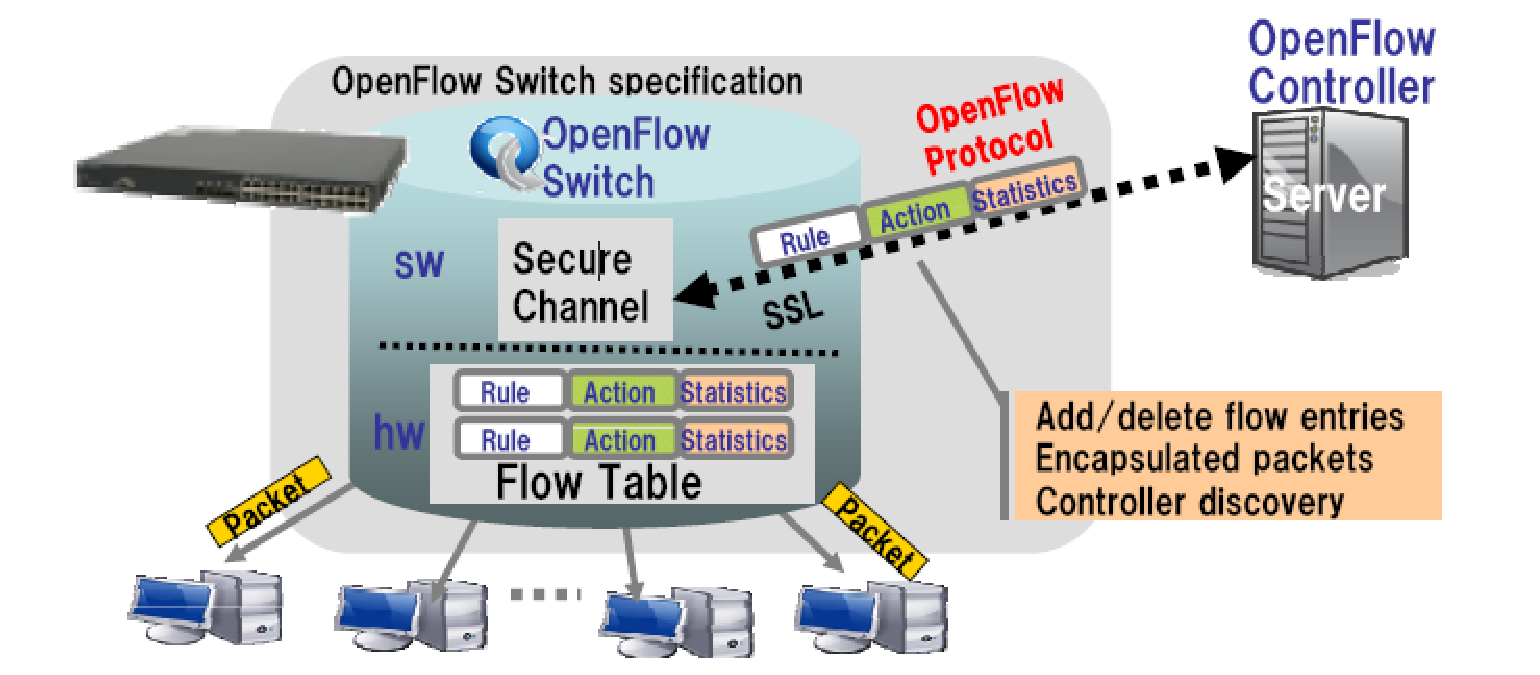
\includegraphics[scale=0.55]{./figuras/openflowComu}
\caption[Esquema de comunicación \emph{OpenFlow}]{Esquema de comunicación \emph{OpenFlow}. Imagen extraída de  \url{https://ltgjamaica.wordpress.com/2012/04/29/software-defined-networking-first-look-at-openflow-30/}}\label{openflowComu}
\end{figure}

Para que esta comunicación se lleve a cabo será necesario hacer uso de múltiples elementos. Una breve descripción de todos estos conceptos puede ser consultada en el capítulo 3 (glosario) de \cite{openflow13}. A continuación se describen algunos de ellos.

\subsubsection{Puertos \emph{OpenFlow}} 

Son las interfaces de red definidas para el envío de paquetes entre \emph{OpenFlow} y el resto de la red. Cada \textit{switch} \emph{OpenFlow} está conectado lógicamente (no necesariamente de forma física) con el resto, mediante sus puertos \emph{OpenFlow}. Esta conexión lógica permite el envío de paquetes entre \textit{switches} \emph{OpenFlow}. Esta conexión debe respetar que el envío de paquetes de realice por los puertos \textit{outPut}, y la recepcción por los puertos \textit{ingress} de los \textit{switches} \emph{OpenFlow}. 

Cuando se recibe un paquete, éste pasa por el proceso \textit{pipeline} definido en \ref{openFlowTables}. Este procesamiento \emph{OpenFlow} decidirá que hacer con dicho paquete. Cada \textit{switch} \emph{OpenFlow} debe ser capaz de soportar tres tipos de puertos: físicos, lógicos y puertos reservados.

Los puertos físicos son aquellos que corresponden con una interfaz hardware física del \textit{switch}. \emph{OpenFlow} permite que los puertos físico realmente hagan uso de virtualización.

Otro tipo de puerto es el lógico. Este puerto no tiene porque corresponder con una interfaz física, sino que puede ser una abstracción de niveles más altos (por ejemplo para agregación de enlaces o túneles). Estos puertos deben poder encapsular paquetes (para identificación) y mapear varios puertos físicos por los cuales realizar acciones. El proceso de implementación de puertos lógicos debe ser transparente para \emph{OpenFlow}, comunicándose con el protocolo como si un puerto físico se tratase. 

A la hora de procesar solo existe una diferencia entre puertos físicos y lógicos, y es la inclusión de un campo extra llamado \textit{Tunnel-ID} para identificación en los puertos lógicos. Por lo demás el procesamiento sigue el mismo flujo.

El tercer y último tipo de puerto corresponde a los reservados. Definidos por la especificación \emph{OpenFlow} y usados para acciones de envío específicas, como transmisión de paquetes hacia el controlador, inundación de paquetes o reenvío usando métodos no \emph{OpenFlow}. Dentro de los puertos reservados existen dos tipos: necesarios y no necesarios.

\subsubsection{Tablas \emph{OpenFlow}.}\label{openFlowTables} Las tablas \emph{OpenFlow} son uno de los elementos más importantes del estándar, a continuación se describen los conceptos más importantes para poder trabajar con dichas tablas. La descripción completa puede ser encontrada en el capítulo 5 de \cite{openflow13}. 

\begin{itemize}

\item[•] \textbf{Proceso \textit{pipeLine}.} Este proceso es el que describe el mecanismo de \textit{matching} y posterior toma de decisiones. Existen dos modos de trabajo diferentes dependiendo del tipo de \textit{switches} (\textit{Only-OpenFlow} u \textit{OpenFlow-Hybrid}). Dado que vamos a trabajar con emulación de \textit{switches} \emph{OpenFlow} nos vamos a centrar en el proceso \textit{Only-Openflow}.

El proceso \textit{pipeline} de cada \textit{switch} \emph{OpenFlow} cuenta con una o más tablas de flujo, que a su vez contienen múltiples entradas de flujo. El proceso define como los paquetes interactúan con estas tablas de flujo de acuerdo al flujo de trabajo que se describe en la imagen \ref{pipeline}. Un \textit{switch} debe tener por tanto al menos una tabla de flujo (o equivalente si es un \textit{switch} híbrido).


\begin{figure}[tb]
\centering
\hspace*{-1.5cm}
\subfigure[Paso de paquetes por los múltiples \textit{match} de las tablas de flujo]{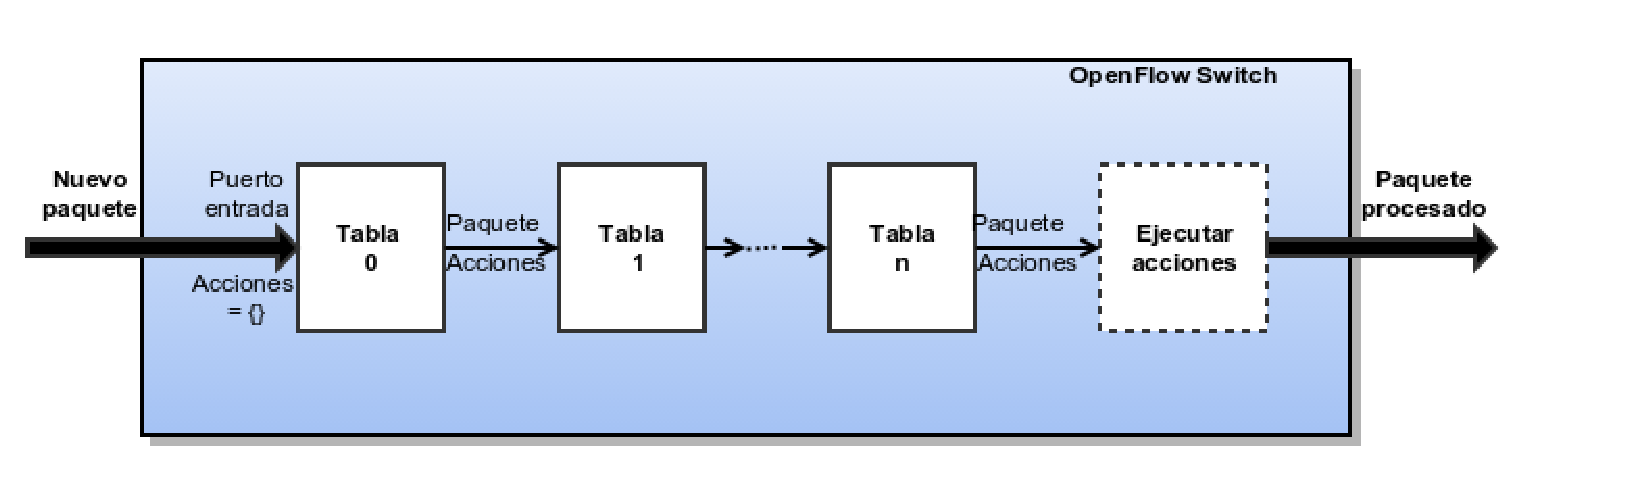
\includegraphics[scale=0.75]{figuras/openflowPipeline}}
\centering
\hspace*{-1.5cm}
\subfigure[Procesamiento de paquete en cada tabla]{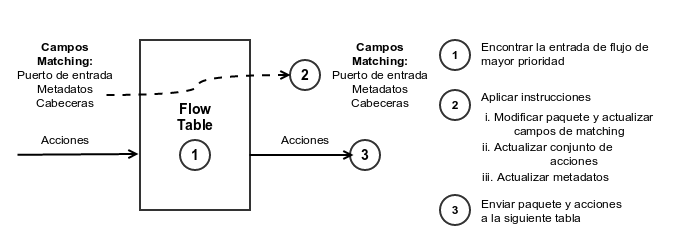
\includegraphics[scale=0.75]{./figuras/openflowPipeline2}}
\caption[Proceso \textit{pipeline}.]{Esquema del procesamiento de paquetes a través del proceso \textit{pipeline}.}\label{pipeline}
\end{figure}

Las tablas de flujo en un \textit{switch} \emph{OpenFlow} están enumeradas en orden ascendente, comenzando siempre por la tabla 0. Un paquete que comienza el proceso \textit{pipeline} siempre comenzará siendo analizado de acuerdo a los flujos instalados en la tabla 0. Dependiendo del resultado obtenido en estaba tabla, el paquete continúa el proceso o finaliza.

El paquete procesado por una tabla de flujo siempre sigue el mismo flujo de operación:

\begin{enumerate}
\item Se intenta realizar \textit{matching} o emparejamiento del paquete con cada flujo en la tabla hasta encontrar una coincidencia, como se verá en \ref{matching}. Hacer \textit{matching} significa que todos los campos de un paquete coinciden con los valores especificados como \textit{match} para un flujo.
\item Si en la tabla no se ha encontrado ninguna entrada de flujo coincidente con el paquete, este pasará a la siguiente tabla. En caso de que si se encuentre dicha coincidencia, pueden darse dos situaciones.

\begin{enumerate}
\item En el primer caso, una vez encontrada la coincidencia, el proceso \textit{pipeline} se detiene en esta tabla, y se llevan a cabo las acciones definidas para los flujos coincidentes.
\item En el segundo caso, si la entrada de flujo tiene definida una acción \textit{Goto-Table}, el paquete debe seguir siendo procesado en otra tabla. En este segundo caso se requiere que siempre que se mande un paquete para ser procesado a otra tabla, el orden de esta tabla sea superior al de la primera (para evitar bucles).
\end{enumerate}
\item En caso de que un paquete no encuentre ningún \textit{match} en las tablas, es traspasado a una tabla denominada \textit{missing table}, que decide que hacer con estos paquetes. Las opciones disponibles son: empezar de nuevo el \textit{matching}, pero ignorando algunos campos para hacerlo más flexible, inundar el paquete en la red o mandarlo al controlador a través del canal de control.
\end{enumerate}

Existen dos casos especiales para el procesamiento de paquetes: si no existe tabla \textit{missing table}, los paquetes son directamente descartados. El segundo caso se da cuando los paquetes tienen un \ac{TTL} inválido, en esta caso son enviados al controlador.

\item[•] \textbf{Entradas de flujo.} Una tabla de flujo está compuesta por entradas de flujo que permitirán aplicar acciones para paquetes que coincidan con los \textit{match} especificados. Una entrada de flujo consiste en los campos que se recogen en la tabla \ref{flowentrie}.

\begin{table}[tb]
\begin{center}
\begin{tabular}{|c|c|c|c|c|c|c|}
\hline 
Match Fields & Priority & Counters & Instructions & Timeouts & Cookie & Flags \\ 
\hline 
\end{tabular}
\end{center}
\caption[Campos de una entrada de flujo]{Campos de una entrada de flujo.}\label{flowentrie}
\end{table}

Estos campos se encuentran definidos en \cite{openflow13}. Los más importantes para nosotros serán: campos \textit{Match Fields} (permiten detectar los diferentes flujos, \ac{RTP}, \ac{TCP}, etc.), \textit{instructions} (indica que se hará con un paquete que coincida con el \textit{matching}) y \textit{timeouts} (definen el tiempo de validez para la entrada de flujo, \textit{idle} o \textit{hard}). Cada entrada de una tabla de flujo está identificada por la prioridad, y el \textit{match} asociado. En caso de estar disponible en la implementación, existe una entrada con prioridad 0 y los campos del matching vacíos, esta es la conocida como la \textit{missing table}.

\item[•] \textbf{\textit{Matching}.}\label{matching} El proceso de \textit{matching} se lleva a cabo para paquete que llega al \textit{switch}. Está descrito en la figura \ref{matchingProcess} y consiste en consultar cada una de las tablas (por orden) y en función de los resultados obtenidos aplicar las instrucciones definidas.

\begin{figure}[tb]
\centering
%\hspace*{-0.5 cm}
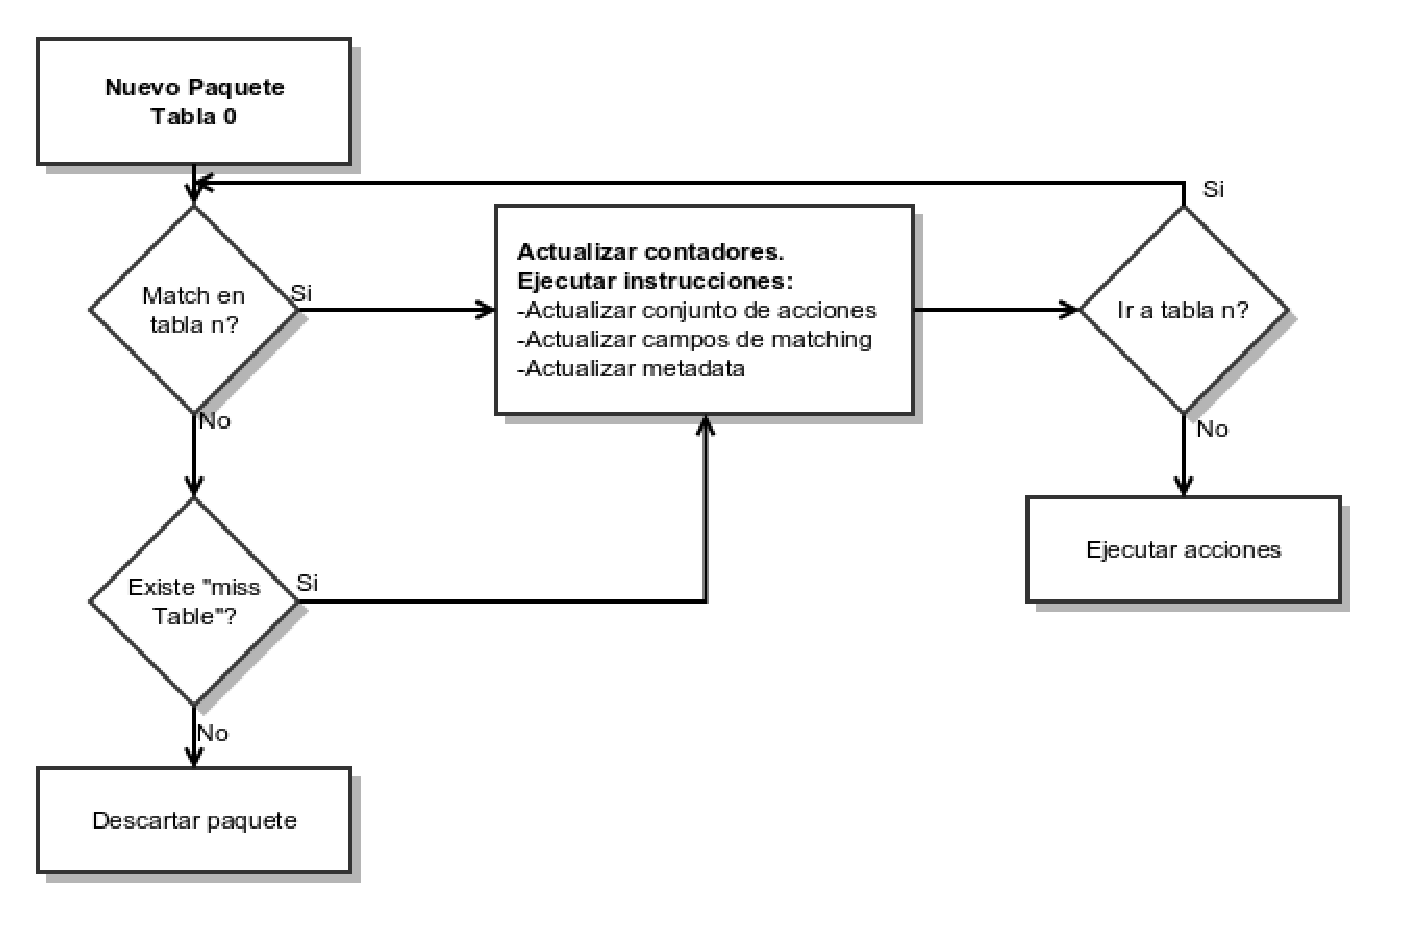
\includegraphics[scale=0.7]{./figuras/matching}
\caption[Proceso de \textit{matching}.]{Procesamiento de paquetes para el \textit{matching}.}\label{matchingProcess}
\end{figure}


Podemos decir que existe \textit{match} para un paquete siempre y cuando todos los campos del \textit{match} definido, sean cumplidos por el paquete, sino el éste continuará el procesamiento. Por defecto los \textit{swicthes} \emph{OpenFlow} traen consigo una serie de campos implementados, pero para cumplir con la especificación solo se requieren los recogidos en la tabla \ref{matchFields}.

\begin{table}[tb]
\centering
%\hspace*{-0.3 cm}
\begin{tabular}{|c|c|}
\hline
\textbf{Campo}     & \textbf{Descripción}                                                 \\ \hline
OXM\_OF\_IN\_PORT  & Puerto de entrada. Puerto físico o lógico del \textit{swtich} \\ \hline
OXM\_OF\_ETH\_DST  & Dirección Ethernet de destino. Puede usar cualquier máscara            \\ \hline
OXM\_OF\_ETH\_SRC  & Dirección Ethernet de origen. Puede usar cualquier máscara                   \\ \hline
OXM\_OF\_ETH\_TYPE & Tipo de paquete Ethernet, tras las etiquetas VLAN       \\ \hline
OXM\_OF\_IP\_PROTO & Protocolo \ac{IP}v4 o \ac{IP}v6                                         \\ \hline
OXM\_OF\_IPV4\_SRC & Dirección origen \ac{IP}v4. Puede usar máscara de subred o no        \\ \hline
OXM\_OF\_IPV4\_DST & Dirección destino \ac{IP}v4. Puede usar máscara de subred o no   \\ \hline
OXM\_OF\_IPV6\_SRC & Dirección origen \ac{IP}v6. Puede usar máscara de subred o no        \\ \hline
OXM\_OF\_IPV6\_DST & Dirección destino \ac{IP}v6. Puede usar máscara de subred o no   \\ \hline
OXM\_OF\_TCP\_SRC  & Puerto origen \ac{TCP}                                                   \\ \hline
OXM\_OF\_TCP\_DST  & Puerto destino \ac{TCP}                                                \\ \hline
OXM\_OF\_UDP\_SRC  & Puerto origen \ac{UDP}                                                        \\ \hline
OXM\_OF\_UDP\_DST  & Puerto destino \ac{UDP}                                                   \\ \hline
\end{tabular}
\caption{\textit{Match Fields} requeridos por \emph{OpenFlow}.}\label{matchFields}
\end{table}

Existe la posibilidad de usar un mayor número de campos o incluir nuevos campos según las necesidades. Por ejemplo entre los campos por defecto se incluyen además algunos que permiten detección directa de etiquetas \ac{MPLS}.

Para más información sobre el proceso de \textit{matching} y ampliar detalles sobre los campos para \textit{match}, se recomienda consultar la especificación \cite{openflow13}, capítulos 5 y 7 respectivamente.


\item[•] \textbf{Contadores.} Los contadores están asociados a cada tabla de flujo, entrada de flujo, puerto, cola u otros elementos. Existe un gran número de contadores posibles, pero \emph{OpenFlow} solo obliga el mantenimiento de algunos, (aunque existen muchos más opcionales). Los contadores obligatorios y de mayor relevancia son los relaciones con el número de entradas (para las tablas). La duración de cada entrada de flujo, paquetes transmitidos y  paquetes recibidos por cada puerto.

\item[•] \textbf{Instrucciones.} Las instrucciones son ejecutadas cuando un paquete finaliza el proceso de \textit{matching} de forma satisfactoria para una entrada de flujo. \emph{OpenFlow} especifica una serie de instrucciones que han de ser soportadas por los \textit{switches}, dejando otras instrucciones como opcionales. Las instrucciones más importantes son aquellas que escriben o borran acciones para cada entrada de flujo, y la instrucción que indica \textit{Goto-Table}, para saltos entre tablas.

\item[•] \textbf{\textit{TimeOuts}.} Los \textit{timeOuts} están definidos para cada entrada de flujo. Existen dos tipos.

\begin{itemize}
\item[•] \textit{IdleTimeOut}, es de tipo \textit{soft} y permite que un flujo sea eliminado de la tabla de flujos tras la ausencia de paquetes coincidentes con el flujo durante el periodo especificado. Cada vez que un paquete hace \textit{match} con esa entrada el contador de tiempo se reinicia.
\item[•] El segundo tipo es \textit{HardTimeOut}, este borrará el flujo siempre que pase el periodo de tiempo establecido, ocurra lo que ocurra (siempre y cuando el controlador no envíe una nueva instrucción que modifique el tiempo o comportamiento).
\end{itemize}
\end{itemize}

\subsubsection{Acciones.} Cada vez que un paquete encuentra una entrada de flujo coincidente, se le asignan una o más acciones. En la especificación están recogidas una serie de acciones (no todas tienen que ser soportadas por los \textit{switches}), de las cuales las más importantes para nosotros son las relacionadas con reenvío y descarte de paquetes.

\begin{itemize}
\item[•] \textbf{\textit{Output}.} Esta acción está asociada al reenvío de paquetes por un puerto \emph{OpenFlow}.
\item[•] \textbf{\textit{Drop}.} Cuando a un paquete se le asocia una acción \textit{drop} tras el procesamiento, éste será descartado.
\item[•] \textbf{\textit{Group}.} Esta acción conlleva el procesamiento del paquete como si fuera de un determinado grupo (consultar Type groupe \cite{openflow13}), permitiendo el procesamiento por grupos de paquetes. Esta definición está diseñada para aumentar la eficiencia de procesamiento.
\end{itemize}

\subsubsection{\textit{OpenFlow Channel} y \textit{Control Channel}.} El canal \emph{OpenFlow} es el que conecta lógicamente los \textit{switches} \emph{OpenFlow} con el controlador. A través de este canal, el controlador configurará y administrará cada \textit{switch} (recibiendo paquetes o enviando órdenes). El canal de control \emph{OpenFlow} puede estar constituido por un solo canal \emph{OpenFlow}, conectado a un controlador, o por varios canales \emph{OpenFlow}, conectados a varios controladores que comparten la administración del \textit{switch}. 

El canal \emph{OpenFlow} exige que todos los mensajes que sean transportados por él, se envíen de acuerdo a la especificación \emph{OpenFlow}, para conseguir la máxima compatibilidad. Este canal suele estar encriptado usando \ac{TLS}, aunque también existe la posibilidad de enviar los paquetes directamente sobre TCP.

El análisis de intercambio de mensajes no tiene cabida en este trabajo, pues no se pretende analizar el funcionamiento interno de \emph{OpenFlow}, sino hacer uso de sus capacidades. Sin embargo es importante destacar que la comunicación entre \textit{switch} y controlador, no tiene porque ser iniciada por ninguna de las dos partes. Por ejemplo un \textit{switch} puede enviar mensajes de forma asíncrona para indicar eventos, sin que estos hayan sido solicitados por el controlador. También pueden existir mensajes simétricos de Hello o Echo por cualquiera de las dos partes, para mantener el canal de comunicación.

El capítulo 6 de \cite{openflow13} contiene todos los mensajes contemplados en el protocolo \emph{OpenFlow} versión 1.3.5 (26 de Marzo de 2015), así como las posibilidades de comunicacińo entre ellos.

Con esto se da por concluido el apartado referente a \emph{OpenFlow}. Se ha pretendido dar las claves de funcionamiento \emph{OpenFlow}. También se ha intentado razonar y justificar el uso de \emph{OpenFlow} como estándar de referencia para redes \ac{SDN}, y haber descrito las claves teóricas que posteriormente nos permitirán desarrollar y alcanzar los objetivos de este trabajo.


\section{Controladores \ac{SDN}}
Uno de los elementos troncales de la arquitectura \ac{SDN} es el controlador, cerebro de toda la arquitectura de red que de él depende. Podemos dividir las diferentes alternativas actuales en dos grandes grupos: controladores de código abierto y controladores comerciales. 

Para el desarrollador independiente, los más interesantes son los controladores abiertos, ya que en ellos podrá desarrollar libremente y contará con el apoyo de la comunidad. Algunos de los controladores comerciales también usan una filosofía de código abierto, con lo que la elección de uno frente a otros será ``complicada".

En este trabajo se requiere el uso de controladores de código abierto que permitan el desarrollo sin coste alguno, se encuentren en desarrollo o en fases finales, y además cuenten con un fuerte apoyo de la comunidad, que permita resolver los problemas que se presenten.

Todas estas razones nos llevan a elegir un controlador de tipo abierto. Sin embargo a continuación se presentan las principales opciones comerciales para evaluar sus capacidades.

\subsection{Controladores comerciales.} 
Este tipo de controladores se encuentran desarrollo (aunque algunos ya son encontrados en soluciones comerciales ofertadas). Surgen como respuesta a la necesidad de un desarrollo rápido y privado frente a los controladores abiertos. Empresas como Cisco y NEC por ejemplo son miembros importantes de algunos de los controladores de código abierto más importantes (como \emph{OpenDayLight}), pero también desarrollan sus propias soluciones comerciales. A continuación se describen brevemente algunas de estas distribuciones comerciales.

\begin{itemize}

\item[•]\textbf{\ac{APIC}.}\cite{apic}. Si se presentó OpFlex como alternativa a \emph{OpenFlow}, se debe tratar el controlador paraeste paradigma diseñado por Cisco. En una infraestructura de red centralizada, \ac{APIC} actúa como un único punto de control central. Proporciona una \ac{API} central, un repositorio central de datos globales y un repositorio de políticas (consultar la sección referida a alternativas \emph{OpenFlow} \ref{opflex}). \ac{APIC} trabaja de forma diferente al resto de controladores \ac{SDN} \emph{OpenFlow}, ya que no se encarga de encaminar cada flujo de datos, sino que según el estado de red, instala políticas en los elementos de red, y serán estos los que se encarguen de tomar decisiones en función de estas políticas.

\item[•]\textbf{\acf{VAN}.}\cite{van}. Es el controlador desarrollado por \textit{HP}. Este si que es un controlador desarrollado sobre \emph{OpenFlow}. Sin entrar demasiado en el funcionamiento interno del controlador, podemos destacar que en el desarrollo de éste está centrado en: incluir seguridad en las comunicaciones del controlador con el resto de la red, administración centralizada, capacidad de automatización y otras capacidades inherentes a redes \ac{SDN}. El esquema que presenta \ac{VAN} no es diferente del usado por \emph{OpenDayLight} u otros controladores, como se puede comprobar en la imagen \ref{van}.

\begin{figure}[tb]
\centering
\hspace*{-1.2cm}
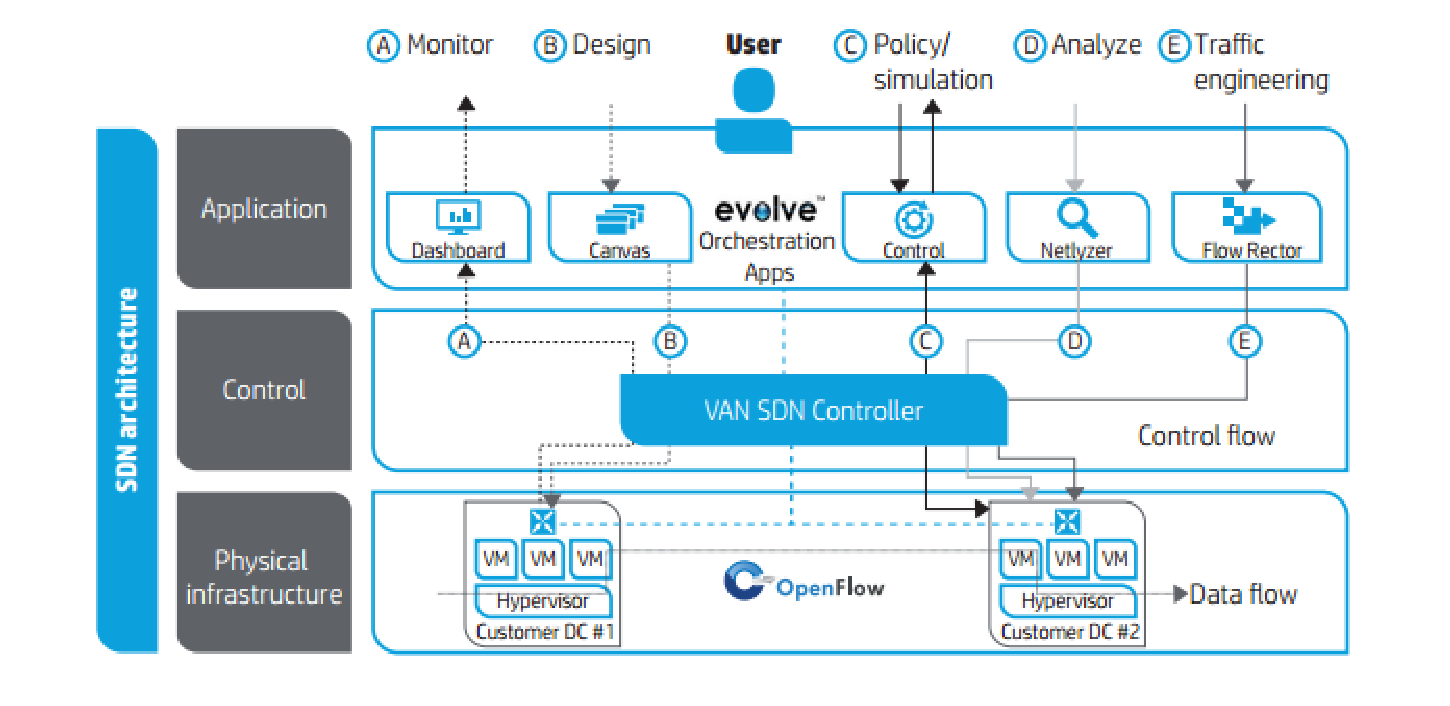
\includegraphics[scale=0.7]{./figuras/van}
\caption[Arquitectura controlador \ac{VAN}]{Arquitectura del controlador \ac{VAN}. Imagen tomada de \url{https://sreeninet.wordpress.com/2014/08/09/sdn-openflow-commercial-applications-part-2/}}\label{van}
\end{figure}

\item[•]\textbf{VMware NSX.} NSX es un controlador desarrollado para la virtualización de redes. Este controlador permite tratar redes físicas como máquinas virtuales, sin importar que implementación física exista debajo. Además integra todas las capacidades propias de virtualización de redes, permitiendo a los clientes obtener todo el potencial de un centro de procesamiento de datos sin necesidad de redes físicas. Además cuenta con propiedades características de redes \ac{SDN}, como la automatización o la naturaleza dinámica y ágil de éstas.
\end{itemize}

Estas son tres soluciones comerciales \ac{SDN}, pero existen muchas más, que sin duda serán capaces de satisfacer las necesidades de los clientes a los que están dirigidas. 

A continuación ponemos el foco en los controladores de código abierto.

\subsection{Controladores de código abierto.} Dentro de los controladores de código abierto existen multitud de alternativas, algunas en fases de desarrollo muy tempranas y novedosas, y otras que ya son referentes en el mercado. En esta sección vamos a describir algunas de ellas apoyándonos en los resultados y conclusiones obtenidas en los artículos \cite{comparativaSDN1} y \cite{comparativaSDN2}. 

No podemos describir todas las alternativas disponibles así que nos hemos centrado en aquellas que consideramos conocidas y que aún se mantienen en desarrollo.

\begin{itemize}
\item[•]\textbf{POX.}\cite{pox}. POX es un controlador hermano de uno de los pioneros, NOX\footnote{\url{http://www.noxrepo.org/}}. POX surge como un intento para conseguir que aquellos usuarios que comienzan con \ac{SDN} se encuentren con un entorno de desarrollo amigable. Este controlador se ha desarrollado sobre Python. POX como controlador que cuenta con dos métodos de desarrollo: el primero es una \ac{API} basada en Python, el segundo método está basado en una \ac{API} vía web que hace uso de JSON-RPC. Por último destacar que además cuenta con una interfaz gráfica vía web (como la mayoría de controladores) desde la cual se puede monitorizar la red y realizar otras operaciones. Como punto negativo hay mencionar que POX no cuenta con demasiado información ni manuales disponibles, siendo algo a valorar por aquellos que deseen comenzar con él.

\item[•]\textbf{Ryu.}\cite{ryu}. Este controlador se define a si mismo como un proveedor de componentes software, con una \ac{API} muy bien definida que permite a los desarrolladores crear nuevas aplicaciones de administración y control de forma sencilla. Uno de los puntos fuertes de Ryu es el soporte de varios protocolos para la administración de equipos, no solo \emph{OpenFlow}. Ryu está desarrollado sobre Python. Como punto negativo debemos destacar la dependencia del S.O. sobre el que se ejecuta (solo se soporta Línux) así como la baja actividad que presentan sus \textit{mailing list}\footnote{\url{http://sourceforge.net/p/ryu/mailman/ryu-devel/}}, en comparación con las de \ac{ODL}. Ryu cuenta con una \textit{wiki} propia, con suficiente documentación como para considerarla de nivel medio, según \cite{comparativaSDN1}. Otro punto que se debe tener en cuenta es que Ryu no depende de miembros externos (como si \emph{OpenDayLight}), con lo que se gana en agilidad y poder de decisión (de los usuarios) pero se pierde soporte y apoyo.

\item[•]\textbf{Trema.}\cite{trema}. Más que un controlador en si, Trema presenta un \textit{framework} de fácil uso, donde desarrollar tu propio controlador \emph{OpenFlow} desde 0. Está escrito en Ruby y C, y pretende ser una alternativa real a controladores en fases de desarrollo avanzadas. Trema puede ser una opción para aquellos que deseen llevar a cabo un proyecto muy específico pues solo se implementarán los módulos necesarios (ganando en eficiencia). Sin embargo el trabajo por parte de los desarrolladores se verá aumentado al tener que diseñar un controlador completo. Trema no cuenta con interfaz gráfica (tendría que ser desarrollada para cada caso) y tampoco tiene soporte para \ac{REST} \ac{API}, capacidad muy demandada por la comunidad de usuarios. La documentación y flexibilidad que podemos encontrar por parte de Trema es buena, sin embargo en sus listas de correo el último tema abierto es del 3 de Marzo de 2015\footnote{Consultado el día 25/05/2015}, no siendo un dato muy alentador para aquellos que decidan iniciarse con un controlador \ac{SDN}.

\item[•]\textbf{FloodLight.}\cite{floodlight} FloodLight se puede presentar como la evolución del controlador Beacon (uno de los primeros controladores \ac{SDN} que surgieron).  Está desarrollado sobre JAVA y al igual que la gran mayoría de controladores posee una interfaz web. Además soporta el uso de \ac{API} \ac{REST}. Otro aspecto importante de Floodlight es la importante comunidad que lo apoya. Los desarrolladores participan de forma muy activa en la lista de correo, con lo que cualquier duda que pueda surgir para nuevos usuarios estará ya resuelta o se resolverá de forma rápida, lo cual como ya se ha comentado es imprescindible. Sin embargo presenta algunos inconvenientes, por ejemplo la dependencia de desarrollo de \ac{API} \ac{REST}. Además la relevancia de FloodLight (pese a contar con apoyos importantes como el de \textit{C}anonical) ha ido perdiendo peso y apenas es relevante frente a \ac{ODL}.

\end{itemize}

Uno de los aspectos más importantes para la decisión sobre que controlador usar es la relevancia actual de éste. En la imagen \ref{controllerTrend} se ve claramente la evolución de los distintos controladores presentados. Los datos que se presentan en la imagen \ref{controllerTrend} están limitados a términos de búsqueda relacionados con Redes, para garantizar la validez y concordancia de estos datos con el ámbito en el que trabajamos.

\begin{figure}[tb]
\centering
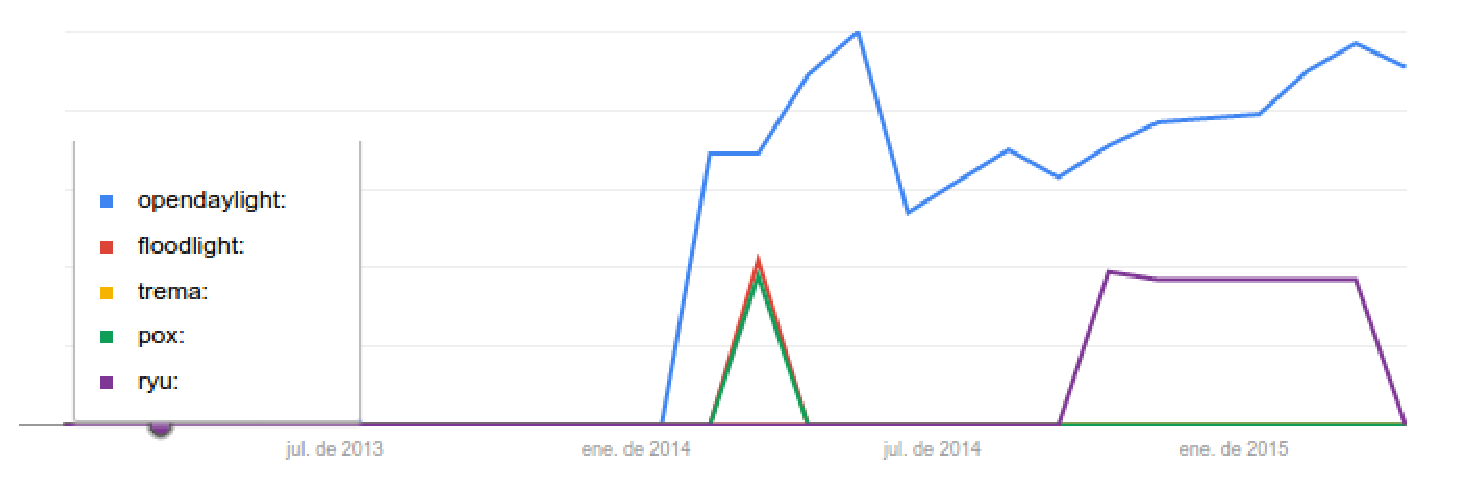
\includegraphics[scale=0.55]{./figuras/controllerTrend}
\caption[Interés de búsqueda de controladores en GooGle]{Interés generado por los diferentes controladores en Google entre 2013 y 2015. Datos tomados de GooGle Trends. Consultado en mayo 2015}\label{controllerTrend}
\end{figure}

Por último se presenta en la tabla \ref{resumen} un resumen sobre los controladores aquí presentados, incluyendo además el controlador \emph{OpenDayLight} que se describe en la sección \ref{opendaylight}.

\newpage

\begin{table}[tb]
\centering
\hspace*{-1.2cm}
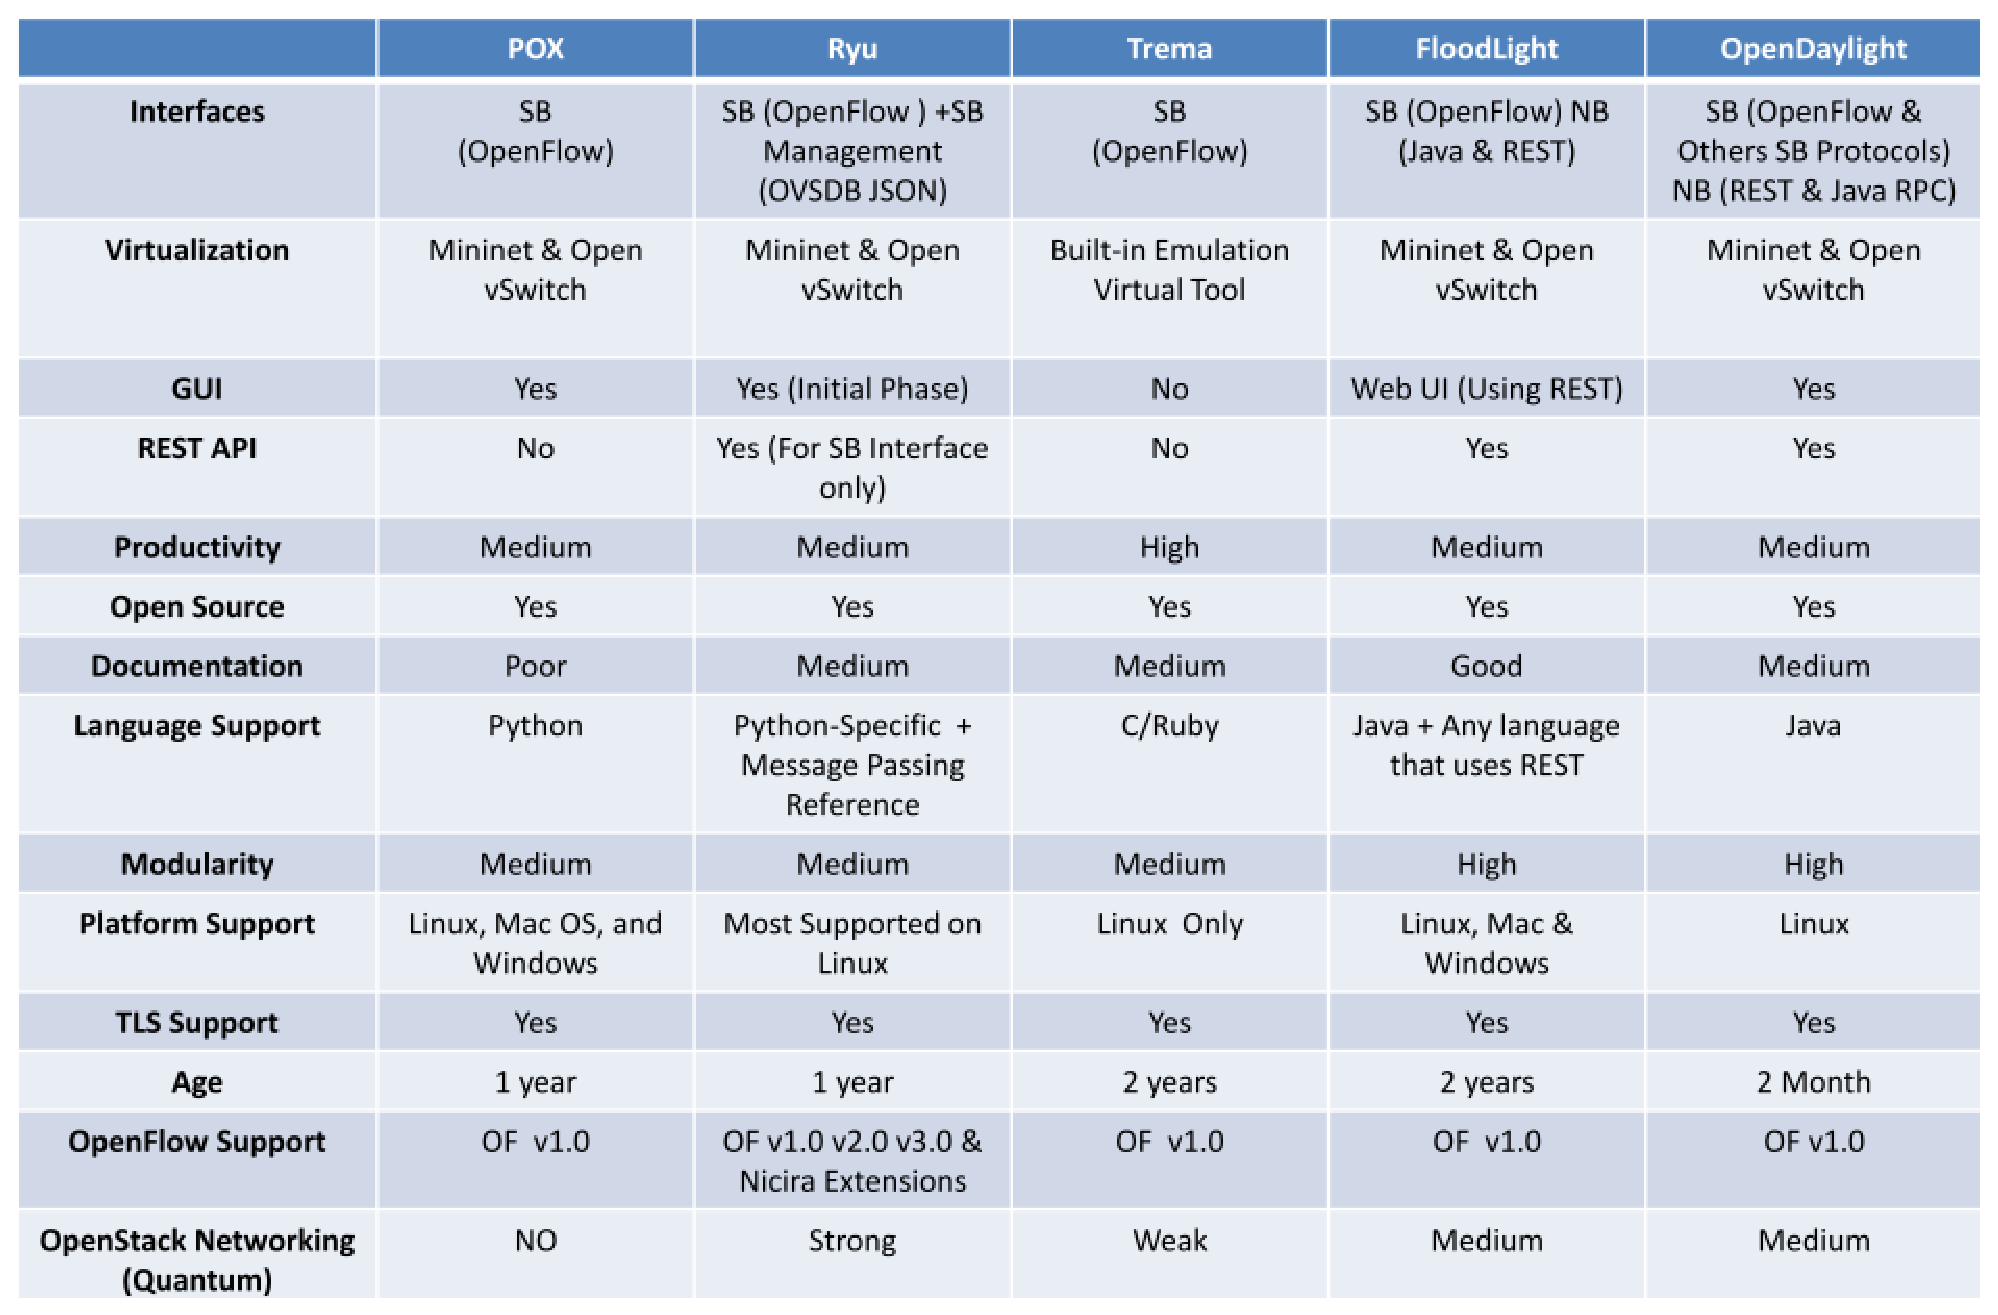
\includegraphics[scale=0.55]{./figuras/comparativaController}
\caption[Resumen controladores SDN]{Resumen controladores SDN. Tabla tomada de \cite{comparativaSDN1}.}\label{resumen}
\end{table}

\subsection{\emph{OpenDayLight}}\label{opendaylight}
\ac{ODL} es el controlador elegido para el estudio y desarrollo de los objetivos marcados en este trabajo. A lo largo de la sección anterior se han descrotp algunos de los puntos débiles del resto de controladores comparados, a fin de justificar el uso de \emph{OpenDayLight}. A modo de resumen se enumeran a continuación las principales fortalezas de \ac{ODL}:

\begin{enumerate}
\item Apoyo de la industria con más de 50 miembros implicados en el proyecto, algunos de ellos de gran relevancia como los que aparecen en la imagen \ref{ODLMembers}.
\item Proyecto bajo la protección de la Línux Foundation y totalmente de código abierto.
\item Desarrollado totalmente en JAVA, con posibilidades de desarrollo de aplicaciones vía varias tecnologías ({API} \ac{REST}, JAVA, \ac{DOM}. \ac{API}).
\item Documentación extensa (aunque con deficiencias aún\footnote{A fecha 15/06/2015.} para aquellos que no están familiarizados). Además cuenta con una comunidad muy activa y con un gran número de usuarios.
\item Proyecto en continuo desarrollo\footnote{Última versión estable \textit{Lithium} lanzada el 29/06/2015.}.
\end{enumerate}

Estas son solo algunas de las razones que justifican el uso de \emph{OpenDayLight}, pero no todas, estamos obviando capacidades más técnicas que se irán desgranando a lo largo de esta sección.

\begin{figure}[tb]
\centering
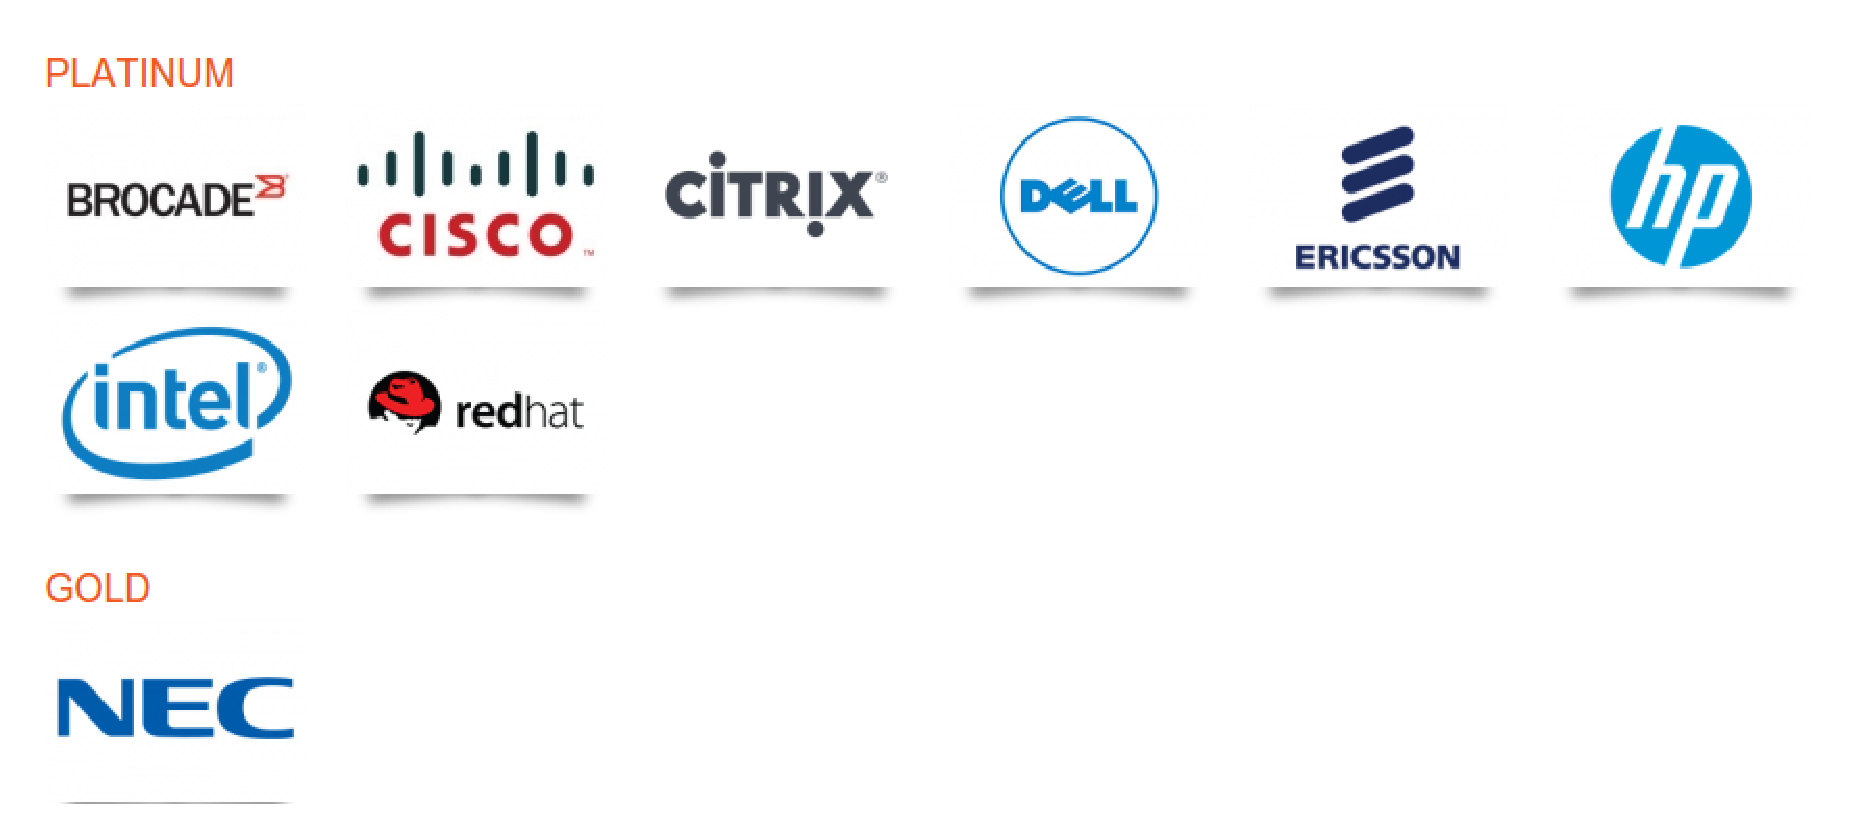
\includegraphics[scale=0.5]{./figuras/ODLMembers}
\caption[\emph{OpenDayLight} Platinum Members]{Miembros platino y oro del proyecto \emph{OpenDayLight}. Imagen extraída de \url{http://www.opendaylight.org/}}\label{ODLMembers}
\end{figure}

\subsubsection{Historia y desarrollo.}
\emph{OpenDayLight} surgió con el objetivo de acelerar la adopción de \ac{SDN}, y crear una base sólida para las funciones de virtualización de red mediante, la colaboración de los pesos pesados del sector. El 8 de Febrero de 2013 se presentó en \textit{SDN Central\footnote{\url{https://www.sdxcentral.com/articles/news/spotlight-on-daylight-sdn-consortium-open-source-controller/2013/02/}}} un consorcio de grandes empresas, bajo una estructura de fundación \textit{open-source}. Posteriormente en Abril de 2013 (coincidiendo con el \ac{ONS} de esa fecha), la Línux Foundation anunció la fundación de \emph{OpenDayLight} como proyecto abierto, con el fin de acelerar la adopción, fomentar la innovación y crear un enfoque abierto y transparente. Dentro de los miembros fundadores se encontraban compañías de gran importancia, tales como Arista Networks, Big Switch, Brocade, Cisco, Citrix, Ericsson, HP, IBM, Juniper Networks, Microsoft, NEC, Nuage Networks, PLUMgrid, Red Hat y VMware. 

Ante este anuncio las reacciones no fueron todo lo positivas como se podía esperar. Por un lado se encontraron aquellas voces que reaccionaron muy positivamente ante los objetivos del proyecto y su estructura abierta. Sin embargo también se dieron opiniones críticas en torno a los miembros del grupo, ya que muchos de estos no desarrollan ni venden hardware relacionado con este tipo de redes, con lo cual se desconfió de los objetivos del grupo, ya que miembros como Microsoft, VMware o Citrix entre otros no son considerados vendedores "históricos" como si lo son Cisco o Juniper.

La primera versión de \ac{ODL} (\textit{Hydrogen}) fue lanzada en Febrero de 2014, incluyendo un controlador de código abierto, capacidades de virtualización y algunos \textit{plugins}. Posteriormente han aparecido distintas versiones que incluían nuevas funcionalidades y mejoras. En Noviembre de 2014 se lanzó una nueva versión que incluía un entorno de trabajo mucho más amigable, basado en \textit{Apache Karaf} y que se constituyó como \textit{Helium}. La última versión estable es la ya mencionada SR3 que mantiene la estructura del proyecto \textit{Helium}\footnote{El 29 de Junio de 2019, se lanza una versión Lithium, la cual no ha podido ser analizada para esta memoria por el calendario de entrega.}.

Antes de finalizar, se debe destacar que cualquier cambio en \emph{OpenDayLight} está sujeto a una votación por parte del comité de dirección técnica. El comité está limitado con un asiento/voto por cada miembro del proyecto, pero no todos los miembros tienen voto. Todos los miembros platino tienen un asiento en la junta independientemente de su colaboración, del resto de miembros, solo aquellos que son considerados importantes, de calidad o con proyectos centrados \emph{OpenDayLight}, serán considerados para obtener un asiento (y por tanto voto) durante el año siguiente al nombramiento. Como conclusión se puede decir por tanto que \emph{OpenDayLight} se asegura su independencia de un solo fabricante hardware. Sin embargo también es cierto que la mayoría del poder (votos) recae sobre los miembros platino.

\subsubsection{Diseño}
\begin{figure}[tb]
\centering
\hspace*{-0.5cm}
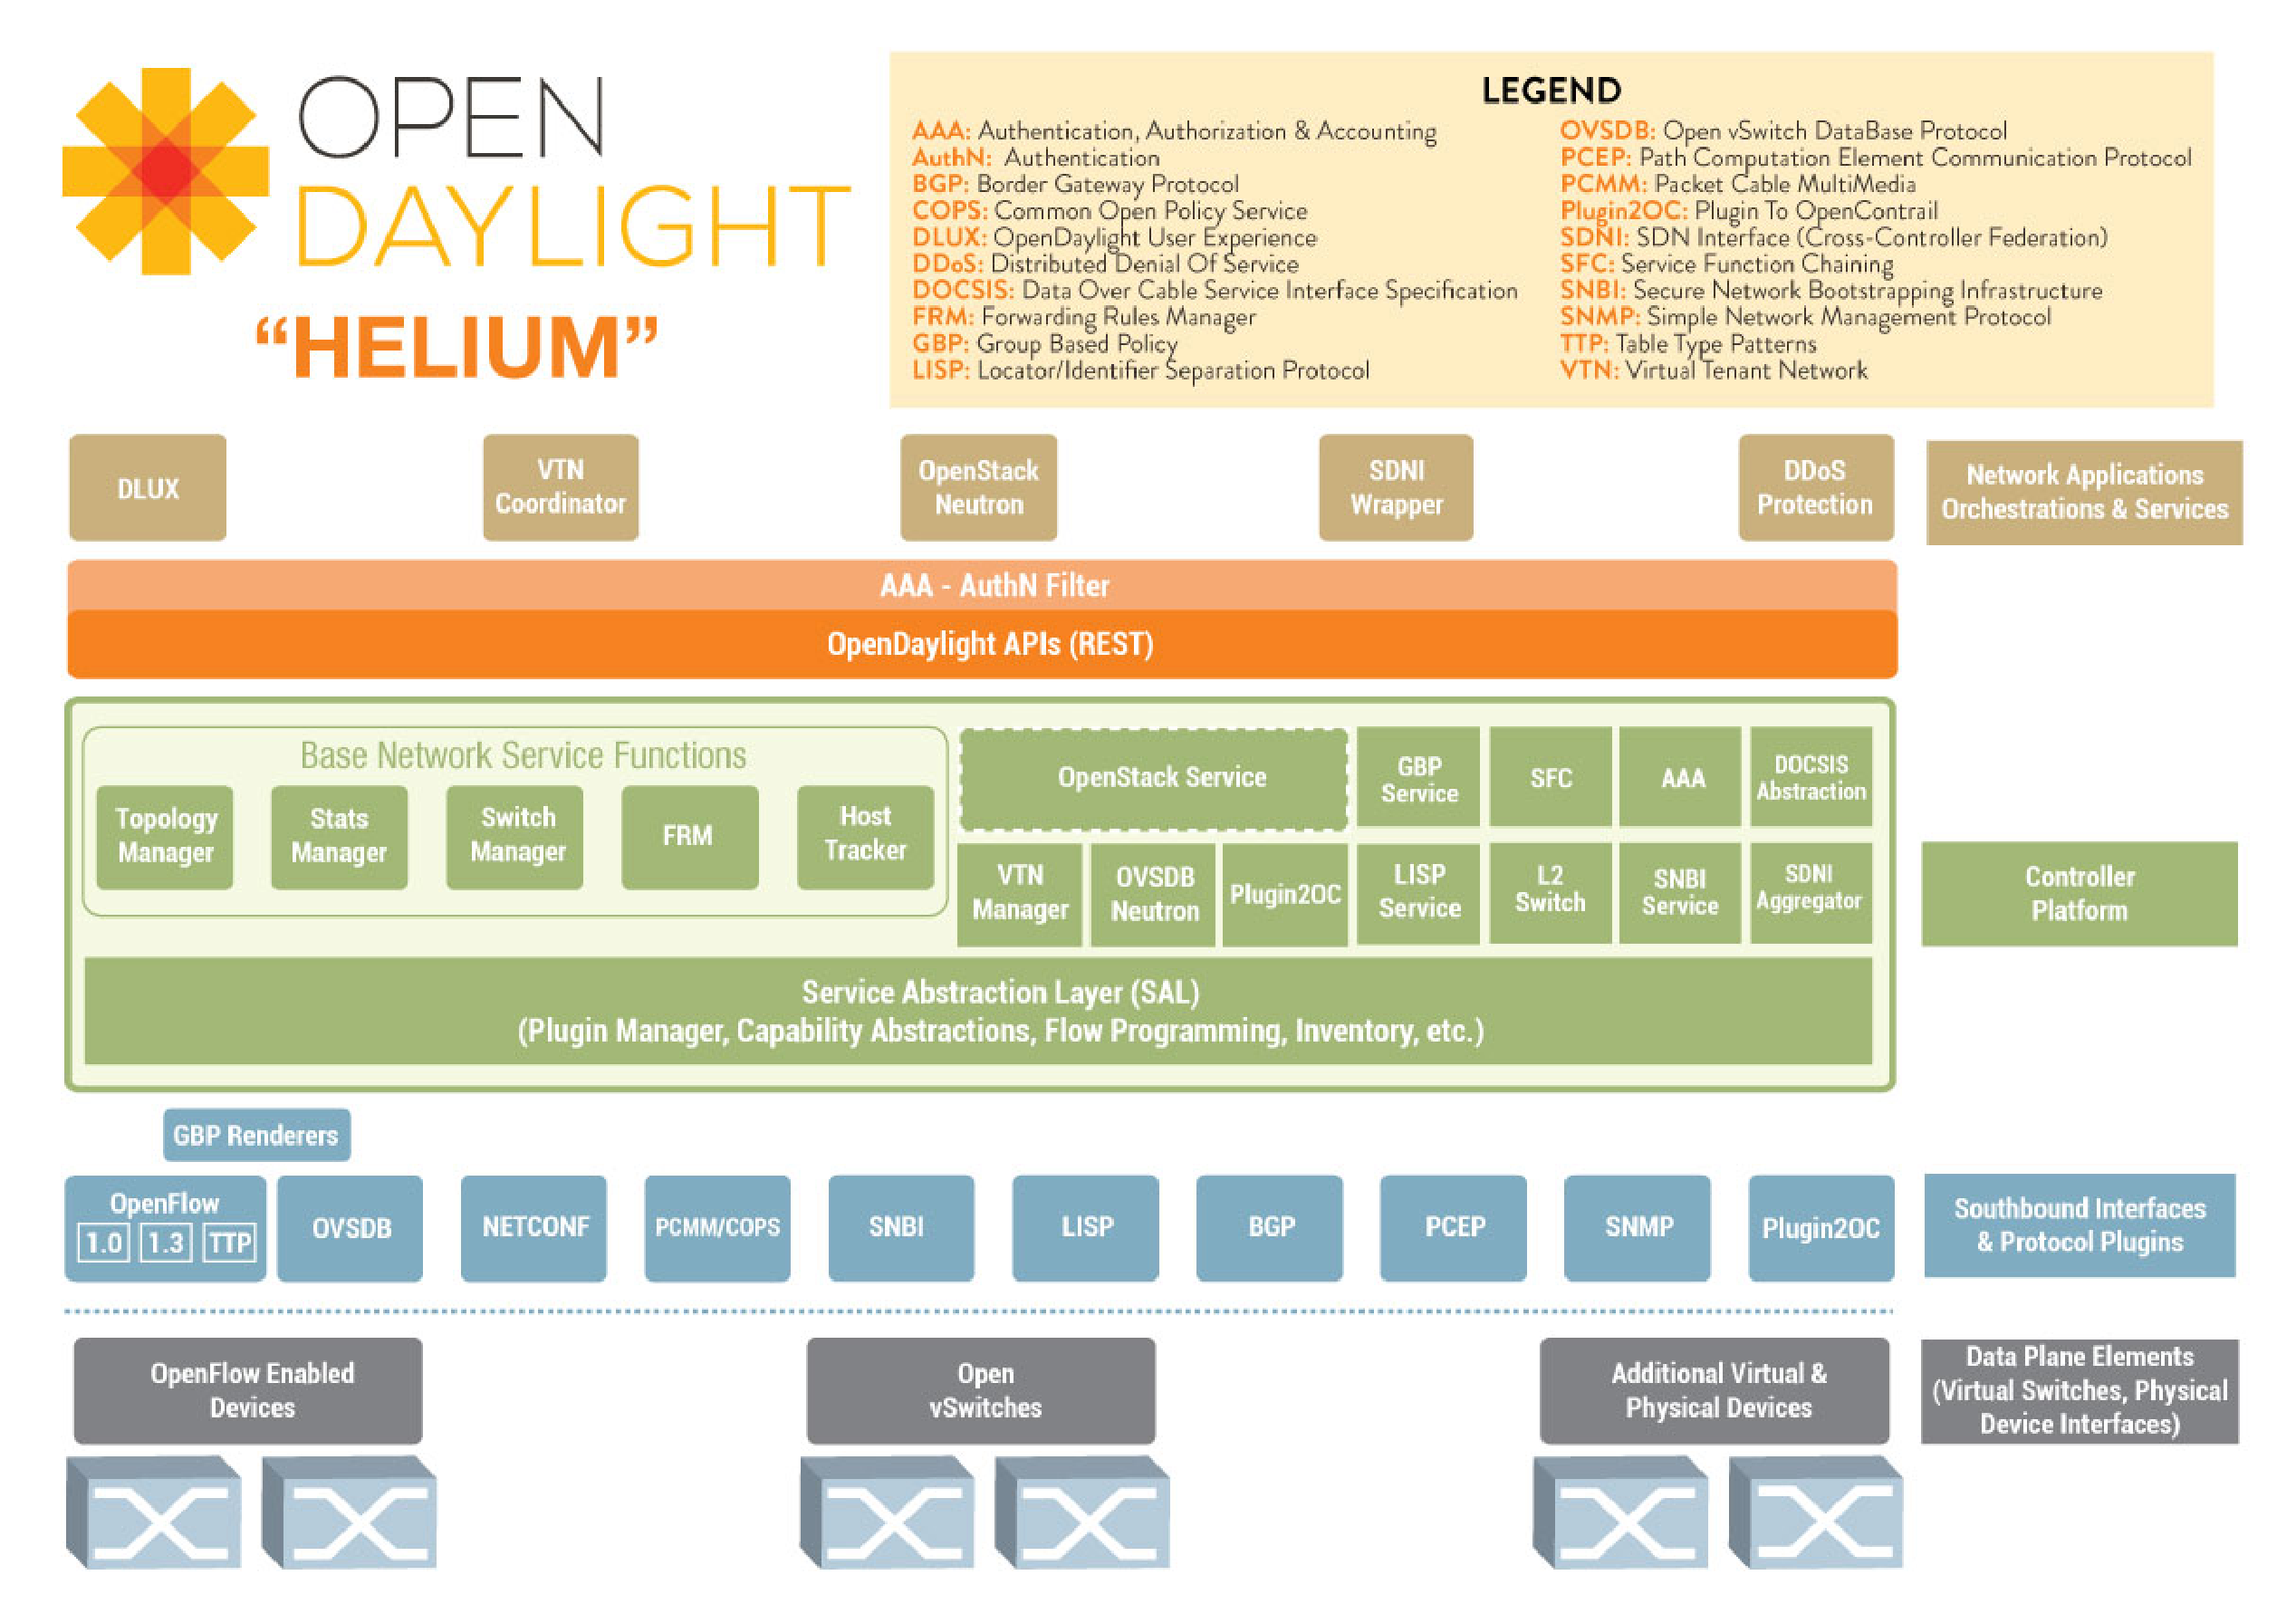
\includegraphics[scale=0.4]{./figuras/ODLOverview}
\caption[Vista técnica del controlador \emph{OpenDayLight}]{Vista técnica del controlador \emph{OpenDayLight}. Imagen tomada de \url{http://www.opendaylight.org/project/technical-overview}.}\label{ODLOverview}
\end{figure}

En la imagen \ref{ODLOverview} podemos encontrar la arquitectura del controlador en su última versión cuya estructura se mantiene como en la versión Hydrogen, aunque se añaden más módulos al núcleo del controlador y la capa de seguridad \ac{AAA}. Se distinguen tres capas en esta arquitectura:

\begin{enumerate}

\item \textbf{Aplicaciones de red e instrumentación.} En la capa de mayor nivel se encuentran las aplicaciones que se encargan del control y monitorización de la red subyacente. También se pueden encontrar en esta capa, soluciones que hagan uso de computación en la nube o servicios de virtualización de red. En esta capa podríamos decir que se encuentran aquellas aplicaciones que computan la ingeniería de tráfico de la red.

\item \textbf{Controlador.} Es la capa central y donde se manifiestan las abstracciones de \ac{SDN}. El controlador cuenta con una serie de módulos implementados que permiten a las aplicaciones de la capa superior obtener datos e información sobre el estado de la red. Además cuenta con una serie de \ac{API}s que permiten el desarrollo de las aplicaciones superiores (\ac{DOM} \ac{API}, \ac{REST} \ac{API} o JAVA), mientras se implementan varios protocolos que permiten la comunicación con los elementos de red inferiores (\emph{OpenFlow}, \ac{BGP}, \ac{PCEP}, \ac{SNMP} entre otros).
 
\item \textbf{Elementos de red físicos y virtuales.} La capa inferior está constituida por aquellos elementos de red que son programables mediante los protocolos implementados por el controlador. Gracias a la capa de abstracción del controlador, se pretende que todos los elementos (de cualquier fabricante) sean compatibles con el controlador \emph{OpenDayLight}.

\end{enumerate}

El controlador \ac{ODL} está implementado en software, haciendo uso de su propia máquina virtual de JAVA. Por tanto su ejecución es independiente del \ac{SO} (siempre y cuando los \ac{SO} soporten JAVA), siendo compatible con la mayoría de \ac{SO} del mundo.

El desarrollo de aplicaciones para \ac{ODL} puede ser llevado a cabo por varias vías gracias a la \textit{Northbound} \ac{API}. Por un lado el controlador soporta el desarrollo mediante el uso del framework \ac{OSGi}\footnote{\url{http://www.osgi.org/Main/HomePage}}. También soporta la comunicación bidireccional usando la \ac{REST} \ac{API}. OSGi será tratado con mayor profundidad en la sección \ref{desarrollo}. El uso de la \ac{API} vía web permite ejecutar aplicaciones que no se encuentran en el mismo dominio de direcciones que el controlador, mientras que \ac{OSGi} se usa para aquellas aplicaciones que si están en el mismo dominio de direcciones. Haciendo uso de cualquiera de los dos métodos, las aplicaciones usan el controlador para recabar información sobre el estado de red, monitorización, etc. Con esta información ejecutan algoritmos inteligentes que posteriormente les permitirán (mediante el uso del controlador de nuevo), la instalación de nuevas reglas para la red subyacente.

En el núcleo del controlador se encuentran una serie de módulos que posibilitan la recolección de estadísticas, visión global de red, estudio de capacidades, etc. Estos módulos son los que permiten a las aplicaciones superiores tener información actualizada para hacer uso de los algoritmos inteligentes. Aparte de estos servicios en el núcleo del controlador, también se pueden encontrar servicios orientados a seguridad y otras extensiones que permiten un mejor control.

Por último destacar que el controlador es totalmente independiente de los elementos de red y protocolos inferiores gracias al uso de la capa de \ac{SAL}, que se encarga de exponer trasladar las peticiones de las aplicaciones de capas superiores hacia abajo, transformando estas peticiones dependiendo del protocolo de comunicación con los dispositivos de red (ya sea \emph{OpenFlow}, BGP-LS o el resto de los soportados).

Se ha descrito brevemente funcionamiento de \emph{OpenDayLight} y como se debe encarar el desarrollo de aplicaciones posteriores a fin de conseguir los objetivos propuestos y realizar un estudio sobre la funcionalidad y capacidad de redes SDN.

En la sección \ref{desarrollo} se tratará con mayor profundidad el modo de desarrollo sobre \ac{ODL} y el funcionamiento interno de este. 

Con esta sección se da por terminado el capítulo dedicado al estado del arte, donde hemos realizado un estudio teórico de las tecnologías implicadas en este trabajo, a fin de conseguir una mejor comprensión que posteriormente permita realizar el desarrollo marcado en los objetivos.

\chapter{Planificación y costes}
Este capítulo describe la planificación temporal y de costes para la realización de este proyecto. La planificación intentará acoger todas las fases de preparación, desarrollo y finalización del proyecto, con el objetivo de al menos igualar la carga de trabajo especificada para la realización de un proyecto de estas características. De igual modo se ha intentado eliminar en la planificación de costes todos aquellos costes prescindibles.

\section{Planificación temporal}

Para la planificación temporal se ha optado por dividir la carga de trabajo en las siguientes actividades.

\begin{enumerate}
\item Revisión bibliográfica. El objetivo de esta primera fase consistirá en la recopilación y comprensión de toda la información que pueda ser de utilidad para el trabajo. Se pretenden adquirir y recopilar aquellos conocimientos útiles para el desarrollo del trabajo. Por ejemplo, en esta fase se intentará adquirir toda la información posible sobre redes \ac{SDN}.
\item Familiarización con el entorno de trabajo. Esta segunda fase se ha diseñado para aglutinar todo el trabajo previo a la implementación del sistema. Por ejemplo, tiempo de configuración del sistema operativo, primeros pasos con mininet o familiarización con éste.
\item Familiarización con el entorno de desarrollo. Para la tercera fase del proyecto se han escogido las tareas de preparación previa a la implementación de la solución. Estudiar las alternativas para la programación de aplicaciones para el controlador, elección de herramientas de desarrollo y ejecución de ejemplos.
\item Diseño de la solución. Durante el desarrollo de esta fase se pretende diseñar una solución óptima para el problema propuesto, describiendo exhaustivamente los módulos en los cuales se dividirá la solución.
\item Descripción de protocolos y algoritmo de encaminamiento. Fase diseñada para el estudio de los protocolos que posteriormente encaminados. En esta fase se incluyen los aspectos de diseño e implementación del algoritmo de encaminamiento elegido.
\item Desarrollo de aplicaciones guiadas. Fase diseñada para la realización de ejemplos guiados para familiarizarnos con el desarrollo de aplicaciones.
\item Implementación de la solución. En la séptima fase del proyecto se pretende acometer la implementación del sistema, así como la solución de posibles problemas derivados de esta implementación
\item Evaluación de la solución propuesta. En la octava fase se llevarán a cabo diferentes evaluaciones, dividas por módulos, para comprobar el correcto funcionamiento de la solución diseñada. Además se reserva en esta fase carga de trabajo para realizar la evaluación sobre la solución completa, es decir, todos los módulos juntos.
\item Elaboración de la memoria técnica del proyecto. En esta última fase se incluye todo lo relacionado con la realización del documento técnico. Se incluyen el tiempo de preparación y conocimiento del lenguaje Látex y la realización técnica del proyecto.
\end{enumerate}

Esta planificación tiene su equivalencia en duración (horas) en la tabla \ref{tab:horas}.

\begin{table}[tb]
\centering
\begin{tabular}{|c|c|}
\hline
{\bf Fase}                                                                          & {\bf \begin{tabular}[c]{@{}c@{}}Carga de trabajo\\ (horas)\end{tabular}} \\ \hline
Revisión bibliográfica                                                              & 100                                                                      \\ \hline
\begin{tabular}[c]{@{}c@{}}Familiarización con \\ entorno de trabajo\end{tabular}   & 120                                                                      \\ \hline
\begin{tabular}[c]{@{}c@{}}Familiarización con\\ entorno de desarrollo\end{tabular} & 20                                                                       \\ \hline
\begin{tabular}[c]{@{}c@{}}Estudio de protocolos\\ y encaminamiento\end{tabular}    & 15                                                                       \\ \hline
\begin{tabular}[c]{@{}c@{}}Propuesta y diseño\\ de solución\end{tabular}            & 20                                                                       \\ \hline
\begin{tabular}[c]{@{}c@{}}Desarrollo de aplicaciones\\ guiadas\end{tabular}        & 5                                                                        \\ \hline
\begin{tabular}[c]{@{}c@{}}Implementación de la\\ solución propuesta\end{tabular}   & 180                                                                      \\ \hline
\begin{tabular}[c]{@{}c@{}}Evaluación de la\\ solución propuesta\end{tabular}       & 20                                                                       \\ \hline
\begin{tabular}[c]{@{}c@{}}Elaboración de \\ memoria técnica\end{tabular}           & 90                                                                       \\ \hline
\end{tabular}
\caption{Planificación temporal del proyecto}
\label{tab:horas}
\end{table}


\section{Estimación de costes}

Esta sección vamos a desglosar los recursos utilizados y el coste que estos implican. Dividiremos los recursos utilizados en: recursos humanos, recursos software y recursos hardware.

\subsection{Recursos Humanos}

Los recursos humanos estám dividos en dos: Cristian Alfonso Prieto Sánchez (alumno/investigador) y D. Juan José Ramos Muñoz (profesor/tutor). Estimamos que el sueldo de un graduado del nivel del alumno que ha realizado el proyecto (recién titulado) puede estar en torno a 15 euros la hora. El sueldo medio de un profesor/doctor se estima en los 30 euros/hora. 

Con estas suposiciones, suponiendo que el profesor/tutor ha realizado un trabajo aproximado de 50 horas (40 horas de tutorización y 20 de revisión del trabajo del alumno) obtenemos un coste total:

\begin{center}
$Coste humano = 570 horasEst \cdot 15 \textup{\euro} /hora + 60 horasProf \cdot 30 \textup{\euro} /hora = 10.350 \textup{\euro} $
\end{center}

\subsection{Recursos software}
En la planificación de costes se ha intentado minimizar el coste total, abogando por el uso de herramientas gratuitas y libres. El coste asociado es de 0 euros, al usar las herramientas que se enumeran a continuación. Además se ha necesitado hacer uso del software \textit{Text-Live} y \textit{Texmaker} para la realización de esta memoria técnica.

\begin{itemize}
\item[•] Ubuntu 14.04.
\item[•] Compilador Látex para Línux y editor Texmaker.
\item[•] \emph{Mininet}.
\item[•] OpenJDK 7.
\item[•] \emph{Wireshark}.
\item[•] Compilador JAVA Maven.
\item[•] \ac{IDE} ATOM.
\item[•] Controlador \emph{OpenDayLight}.
\item[•] Software emisión \ac{RTP}. \item[•] \textit{Mausezahn} y \textit{VLC}.
\item[•] Captura de vídeo software. \textit{SimpleScreenRecorder}. 
\end{itemize}

\subsection{Recursos hardware}
Serán necesarios los recursos físicos especificados en la tabla \ref{tab:recursos}.

\begin{table}[tb]
\centering
\begin{tabular}{|c|c|c|}
\hline
{\bf Recurso}                                                                & {\bf Período de uso} & {\bf Coste}                                                                 \\ \hline
Equipo personal                                                              & 12 meses             & 750 \euro                                                                \\ \hline
Acceso Internet                                                              & 12 meses             & $25 \textup{\euro} \cdot 12$                                                                   \\ \hline
\begin{tabular}[c]{@{}c@{}}Acesso IEEE\\ (artículos académicos)\end{tabular} & 12 meses             & \begin{tabular}[c]{@{}c@{}}Gratuito\\ (convenio universitario)\end{tabular} \\ \hline
\end{tabular}
\caption{Estimación de costes en recursos hardware.}
\label{tab:recursos}
\end{table}

\subsection{Presupuesto final}
En total se obtiene un coste total de 11.400 \euro para la realización completa del proyecto, donde se han incluido todos los recursos necesarios, tanto humanos como software y hardware.

%%%%%%%%%%%%%%%%%%%%%%%%%%%%%%%%%%%%%%%%%%%%%%

%%%%%%%%%%%%%%%%%%%%%%%%%%%%%%
%
% Capítulo de diseño:
%
%%%%%%%%%%%%%%%%%%%%%%%%%%%%%
\chapter{Diseño de la solución}\label{design}

En este capítulo se definirán los elementos que posteriormente conformarán la solución propuesta. Para ello se detallará el diseño software que regirá el comportamiento del sistema, dividiendo en secciones los tres componentes de la propuesta que se han considerado de mayor importancia (algoritmo de encaminamiento con calidad de servicio, recogida de estadísticas de red, instalación de rutas y recuperación antes cambios de topología).


%jjramos muevo sección a implementación

% introducción... esbozamos la solución
\section{Introducción}
 La solución diseñada en este proyecto se basa en aprovechar la potencia que ofrece disponer de un controlador \ac{SDN} centralizado, que tiene una visión global de toda la red, para poder desplegar rutas que satisfagan los requisitos de calidad de experiencia (\ac{QoE}) de varios flujos multimedia.
 
 Concretamente, se ha diseñado un protocolo de encaminamiento de \emph{estado de enlace}, para generar las rutas por cada flujo multimedia que llegue a la red \ac{SDN}. Para ello, el protocolo de encaminamiento toma como costes distintas métricas, que dependen del tipo de flujo para el que se crea la ruta. Así, tras identificar el tipo de un nuevo flujo, se calculará y configurará una ruta a su destino, que minimice los parámetros de red que degradan la calidad que percibirá el destinatario.
 
 La solución propuesta se compone de varios elementos, que también han sido debidamente diseñados:
  
 \begin{itemize}
  \item[•] Clasificación de flujos paquetes (Sec. \ref{sec:clasificacion-flujos}). Para poder seleccionar la ruta que mejor se ajuste a los requisitos de QoE de un flujo de paquetes, es necesario identificar a qué tipo de aplicación corresponde dicho flujo. 
  \item[•] Algoritmo de encaminamiento (Sec. \ref{sec:algoritmo-encaminamiento}). Una vez reconocido el tipo de flujo, es necesario ejecutar un algoritmo que proporcione una ruta hacia el destino del flujo. Los parámetros de \ac{QoS} de los enlaces que componen dicha ruta debería maximizar la calidad que el usuario final al que va destinado el flujo percibirá. Para ello hace falta estimar previamente cuál es el coste de cada enlace para el algoritmo.
  \item[•] Definición de la matriz de costes por enlace (Sec. \ref{costes}). El algoritmo seleccionado para construir las rutas para cada flujo necesita una representación de la red (qué \emph{switches} y qué enlaces existen). Esta representación será la matriz de costes. Para calcular dicha matriz, es necesario definir una métrica de calidad que se base en los parámetros objetivos de cada enlace, y que tenga en cuenta el tipo de flujo que debe seguir dicha ruta.
  \item[•] Estimación de los parámetros de calidad de servicio por enlace (Sec. \ref{sec:parametros-calidad-servicio}). Para extraer los parámetros objetivos de calidad de cada enlace, es necesario definir cómo calcularlos a partir de la información que proporciona cada \emph{switch}.
 \end{itemize}

 
 Cada uno de estos elementos se describen a continuación.

%%%%%%%%%%%%%%%%%%%%%%%%%%%
%
\section{Clasificación de paquetes}
\label{sec:clasificacion-flujos}

Dentro del desarrollo de este trabajo se necesita evaluar el desarrollo con tipos de tráfico acordes a las necesidades y objetivos que se han planteado hasta ahora. A fin de conseguir este objetivo, se considerarán los tipos de flujo siguientes: flujos \acf{TCP}, \cite{rfcTCP}) o \acf{UDP}, \cite{rfcUDP}), vídeo sobre \acf{RTP}, \cite{rfcRTP}), voz sobre \acf{RTP}, y tráfico \acf{ICMP}, \cite{rfcICMP}).
 
Hay que tener en cuenta que, aunque los \emph{switches OpenFlow} pueden clasificar los paquetes por varios campos de la trama \emph{Ethernet} que reciben, este análisis está limitado por los campos definidos en la especificación \emph{OpenFlow}, \cite{openflow13}. Por ello, aprovechando que cuando llega el primer paquete de un flujo nuevo se le consulta al controlador qué hacer con él, será el controlador, que sí puede procesar en detalle el paquete recibido, el que identifique de qué tipo se trata.
  
En esta sección se tratará la detección de cada uno de estos tipos de tráfico. Si bien, algunos tipos de flujos pueden ser fácilmente identificables mirando las cabeceras del protocolo \ac{IP}, (\cite{rfcIP}), otros como los flujos de vídeo necesitan que ser analizados con más detalle para poder determinar su tipo.

La toma de decisiones del algoritmo de clasificación se lleva a cabo de acuerdo al diagrama mostrado en \ref{packetType}, y está orientado a minimizar la carga en el controlador en función de la carga de tráfico que supone cada uno de estos tipos. Esta minimización pretende aumentar la eficiencia del controlador para mejorar el servicio ofrecido. Atendiendo al diagrama \ref{packetType}, primero se diferencian los paquetes de tipo \ac{RTP}, primero vídeo y posteriormente audio. En tercer lugar se situaría la detección de tráfico \ac{TCP} y por último \ac{ICMP}. Esta organización está basada en la suposición de requerimientos de ancho de banda de cada tipo de tráfico, es decir, hemos supuesto que en la red el número de paquetes \ac{RTP} será mucho mayor al resto, con lo que será más probable que un nuevo paquete que llega al controlador sea de tipo \ac{RTP} vídeo. Lo que se pretende conseguir es que un paquete de vídeo no deba pasar por el proceso de identificación de tipo \ac{ICMP} o \ac{RTP}.
 
\begin{figure}[tb]
\centering
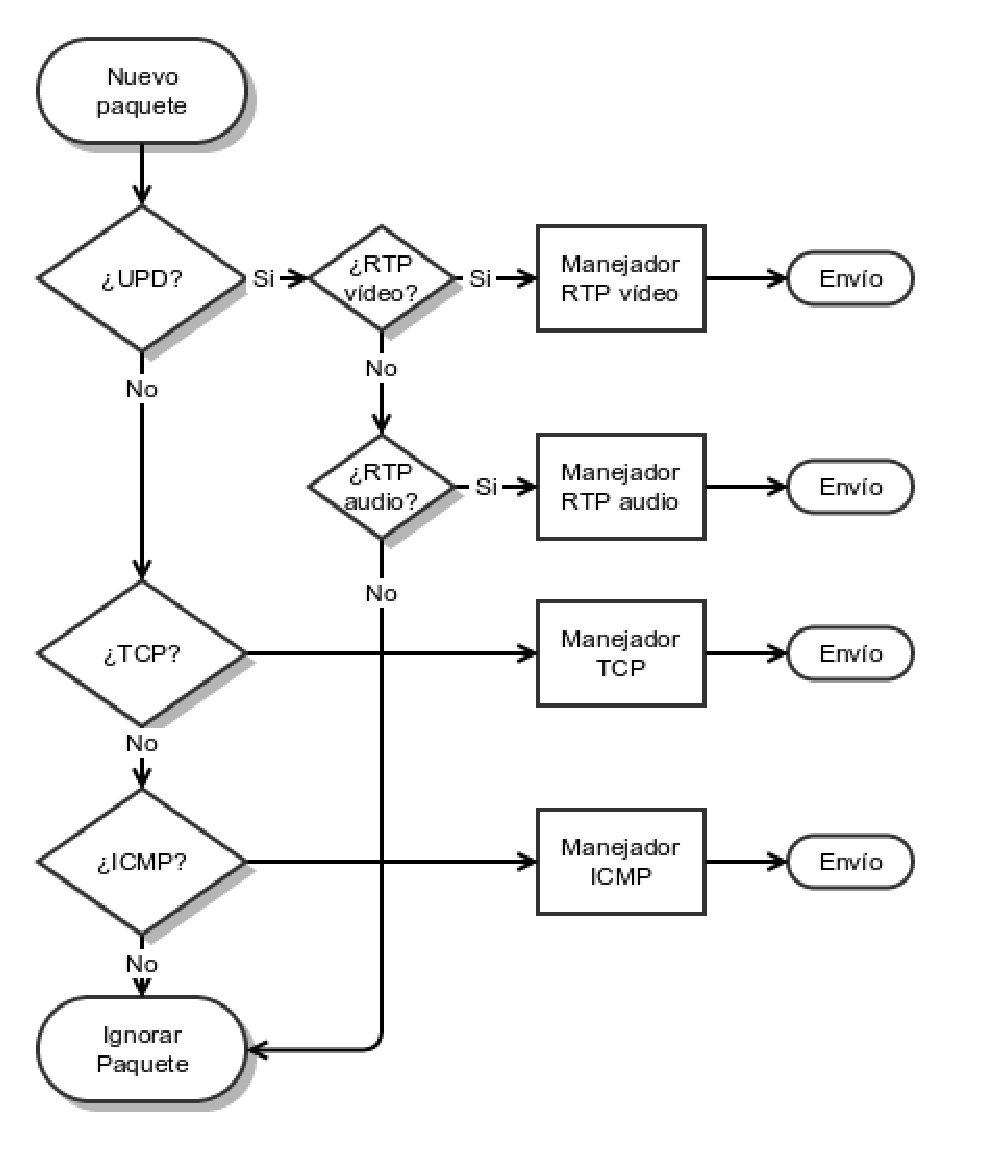
\includegraphics[scale=0.5]{./figuras/packetType}
\caption[Clasificación de paquetes.]{Procedimiento de clasificación de los flujos de paquetes.}
\label{packetType}
\end{figure}

%%%%%%%%%%%%%%%%%%%%%%%%%%%%%%%%%%%%
\subsection{Identificación de tráfico \acs{TCP} y \acs{UDP}}

La identificación de este tipo de tráfico se puede extraer del campo \emph{identificador de protocolo} de la cabecera de los datagramas IP \cite{rfcIP}. La \acs{API} (\emph{Application Programming Interface}) JAVA del controlador \emph{OpenDayLight} hace esta identificación automáticamente. Por ello, la decisión sobre si el tipo de paquete es \ac{UDP} o \ac{TCP} se realizará mediante métodos proporcionados por la \emph{API} usada, (\cite{ciscojavadoc}).

%%%%%%%%%%%%%%%%%%%%%%%%%%%%%%%%%%%%
\subsection{Identificación de vídeo sobre \ac{RTP}}

 Para identificar tipos de flujo de vídeo es necesario analizar la cabecera \ac{RTP} y comprobar que el campo de \emph{tipo de carga} (\emph{Payload Type}, \cite{rfcRTP}), corresponda con el de alguno  de los codificadores de vídeo que consideraremos en el proyecto. Además, para seleccionar con más precisión los flujos de aplicaciones concretas, se comprobará también el puerto al que va destinado. En nuestro caso, los paquetes de vídeo se envían al puerto 5004. Con estas dos condiciones, se puede crear una regla de emparejamiento en las tablas de los \emph{switches} \emph{OpenFlow} para identificar el flujo de vídeo detectado, que incluya sólo las direcciones \ac{IP} y puertos del paquete. Una vez que se han instalado los flujos en los \textit{switches}, estos encaminarán los paquetes correspondientes consultando en sus cabeceras tan solo el protocolo de transporte (\ac{UDP}), el puerto de destino, además de las direcciones de origen y destino \ac{IP}. El proceso de detección que se sigue es el siguiente:

\begin{enumerate}
\item Lo primero que se comprueba es si se trata de tráfico \ac{UDP}.
\item Una vez comprobado que estamos ante tráfico \ac{UDP}, se llama a la función que determinará a cuál de los tipos admitidos corresponde.
\item La función para vídeo comprueba dos requisitos:
\begin{enumerate}
\item Primero comprueba que el puerto de destino es el 5004.
\item A continuación comprueba los campos señalados en la figura \ref{RTPPayload}, analizando si tienen el código estandarizado para vídeo \ac{RTP} sobre \ac{MPEG} \cite{rtpMPEG}. El primer valor consultado debe corresponder a la versión, que actualmente tiene valor 2. El segundo campo que se consulta es el correspondiente al tipo de carga, que para MPEG es el 33\footnote{Especificación RTP. \url{http://www.ietf.org/proceedings/48/I-D/avt-rtp-mp2t-00.txt}}.

%%%%%%%%%%%%%%%%%%
\begin{figure}[tb]
\centering
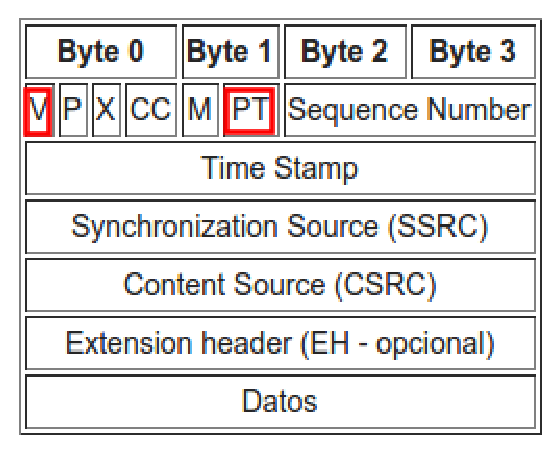
\includegraphics[scale=0.8]{./figuras/RTPPayload}
\caption[Cabecera RTP.]{Cabecera RTP. Imagen tomada de \url{https://tools.ietf.org/html/rfc3550}.}\label{RTPPayload}
\end{figure}
%%%%%%%%%%%%%%%%%%

\end{enumerate}
\end{enumerate}

%%%%%%%%%%%%%%%%%%%%%%%
%
\subsection{Identificación de voz sobre \ac{RTP}}
La detección de paquetes de voz sigue un proceso muy parecido a los paquetes de vídeo. Sin embargo, en este caso, el puerto de destino al cual se envían los paquetes es el puerto 30000. Además, el tipo de carga útil de los paquetes \ac{RTP} coincide con un estándar para voz, el G.711 definido por la \ac{ITU} para la transmisión de voz \cite{ituG711}. Esta codificación coincide con el tipo 0 en \ac{RTP}, definida en el RFC 3551\footnote{\url{https://tools.ietf.org/html/rfc3551}.}.

%%%%%%%%%%%%%%%%%%%%%%%
%
\subsection{\ac{ICMP}}
\ac{ICMP} es un tipo de tráfico distinguido tanto por los \textit{switches} OpenFlow como por el controlador \emph{OpenDayLight} (incluyendo constantes de identificación \ac{ICMP}), con lo que la detección de este tipo de tráfico no va más allá de la llamada a un método de la JAVA \ac{API} que devolverá si el tipo de tráfico es \ac{ICMP} o no.


%%%%%%%%%%%%%%%%%%%
%
%
\section{Protocolo de encaminamiento}
\label{sec:algoritmo-encaminamiento}

Uno de los problemas y a la vez objetivos de nuestro proyecto es el diseño de un sistema capaz de conseguir la mejor ruta dependiendo de los requisitos de \ac{QoS} de varios tipos de tráfico. En esta sección se pretenden dar las claves a partir de las cuales se consigue calcular el camino más apropiado (más rápido, con menos pérdidas o más corto), según el tipo de tráfico a encaminar. Esto se conseguirá a través de la aplicación de dos elementos: un algoritmo de encaminamiento, y una función de cálculo de coste de rutas.

%%%%%%%%%%%%%%%%
\subsection{Algoritmo de encaminamiento}

En una red SDN es el controlador el que toma las decisiones relacionadas con la infraestructura de red. Estas decisiones se toman de forma lógicamente centralizada, ya que además en el controlador dispone de la información de la topología de red.
Por ello, es adecuado elegir un algoritmo de encaminamiento centralizado que aproveche el conocimiento completo de la topología de red para crear rutas de menor coste. Concretamente, nuestro diseño contempla aplicar el algoritmo de \textit{Dijkstra} para identificar las rutas óptimas.

\textit{Dijkstra} es un algoritmo diseñado para determinar el camino más corto (o de menor coste) entre dos vértices de un grafo. \textit{Dijkstra} no es el único algoritmo de encaminamiento existente, pero si que es uno de los más conocidos, usados e implementados, lo cual es una ventaja a la hora de aplicarlo en nuestro desarrollo. Otro algoritmo adecuado a nuestro problema sería el de \textit{Bellman-Ford} \cite{bellmanford}. El inconveniente de usar el algoritmo de \textit{Bellman-Ford} es que tiene un tiempo de procesamiento mayor, lo cual lo hace una opción menos apta para nuestro diseño. 
 Otros algoritmos como los de \textit{Johnson} \cite{johnson} o \textit{Floyd-Warshall} \cite{floydwarshall} también podrían ser aplicados en esta solución. Sin embargo, estos dos algoritmos se diferencian en que en lugar de devolver el camino más corto entre dos vértices de un grafo, devuelven los caminos más corto entre todas las parejas de vértices de la red. Estos algoritmos parten con ventaja en redes estáticas, pero dado que nuestro desarrollo pretende demostrar la viabilidad de utilizar \ac{SDN} para reconfigurar rápidamente una red cambiante, no parece muy lógico usar algoritmos más lentos que tendrán que ser recalculados tras cada cambio. Una vez justificado el uso de este algoritmo sobre otros, conviene entender el modo de funcionamiento.

La idea en la que se basa es explorar todos los caminos más óptimos que parten desde un vértice origen hacia el resto, descartando las rutas que no son prometedoras. Una vez hallados todos los caminos más óptimos, el algoritmo se detiene, obteniendo como resultado el camino más óptimo desde un vértice origen a todos los demás. El ejemplo expuesto a continuación ilustra el modo de funcionamiento del algoritmo.

Partamos de un grafo de red con un coste asociado a cada enlace como en la figura \ref{fig:dijkstra1}.

%%%%%%%%%
\begin{figure}
\centering
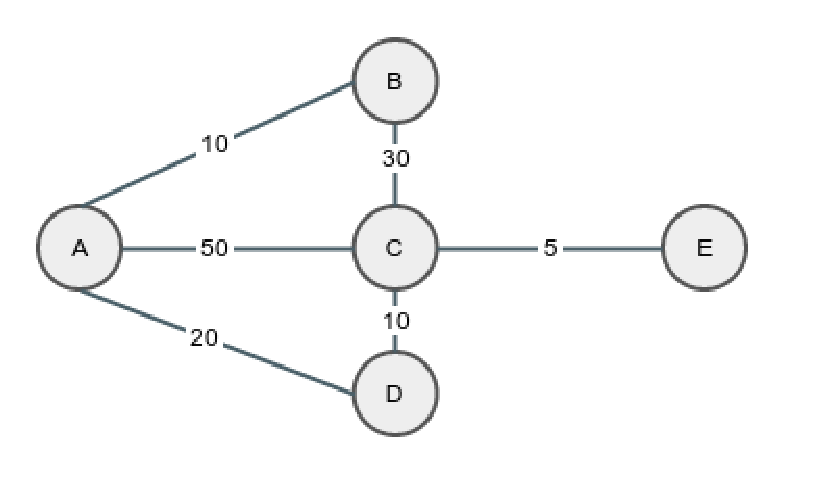
\includegraphics[scale=0.5]{./figuras/dijkstra1}
\caption[Grafo Inicial. \textit{Dijkstra}.]{Grafo de una topología de red con costes asignados a los enlaces.}
\label{fig:dijkstra1}
\end{figure}
%%%%%%%%%

El objetivo será encontrar el camino de menor coste entre los nodos A y E. Si se usase el algoritmo de \textit{Dijkstra} (o cualquier otro) sin ponderar el coste de cada enlace, es decir, suponiendo que todos los enlaces tienen el mismo coste, obtendríamos el camino de la figura \ref{dijkstraMal}, A-C-E, que no es el de menor coste, sino el más corto.

%%%%%%%%%%
\begin{figure}
\centering
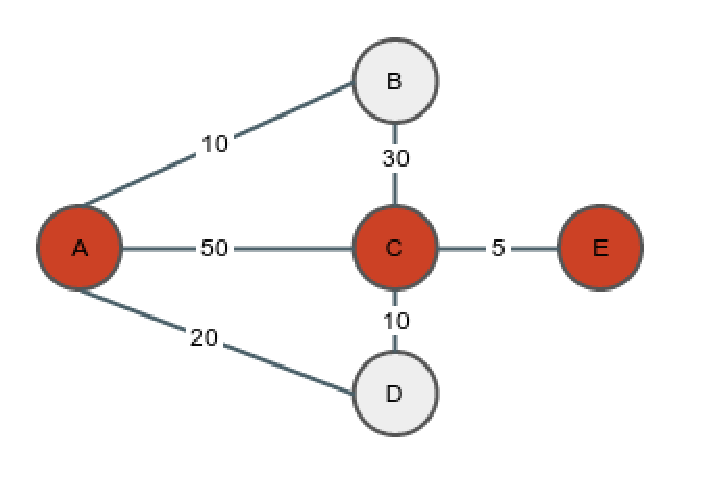
\includegraphics[scale=0.5]{./figuras/dijkstraMal}
\caption[Resultado aplicación sin costes.]{Solución aplicación del algoritmo sin consideraciones de costes.}\label{dijkstraMal}
\end{figure}
%%%%%%%%%

Usando \textit{Dijkstra} pesado con costes que estén relacionados con los parámetros de \ac{QoS} oportunos para cada tipo de tráfico, se obtendría un camino mejor. Por ejemplo, si en el caso presentado en la figura \ref{fig:dijkstra1} los costes de cada enlace correspondieran a su retardo de transmisión, para una aplicación con requisitos de tiempo real, obtendríamos la ruta óptima de mínimo retardo, A-D-C-E. Un desarrollo paso a paso del algoritmo se puede encontrar en el apéndice \ref{dijkstraPaso}, donde se pueden comprobar paso a paso cada una de las iteraciones que nos llevan hasta el resultado deseado.

 Otra de las características de \textit{Dijkstra} que puede ser útil para nuestro diseño, es que es capaz de aplicarse sobre grafos dirigidos. Es decir, es capaz de hallar el mejor camino considerando enlaces con dos sentidos, lo que (aunque en nuestro desarrollo actual no tenga un gran peso), es muy útil en redes que no tienen características simétricas en los enlaces de subida y de bajada.
 
 De cualquier manera, para poder aplicar el algoritmo de encaminamiento, es necesario definir los costes de los enlaces de la red mediante una matriz de costes. Dichos costes dependerán del tipo de tráfico que deba seguir la ruta calculada por \textit{Dijkstra}.  

%%%%%%%%%%%%%%
\subsection{Estimación de la matriz de costes} 
\label{costes}

La estimación de costes de enlaces es uno de los puntos de mayor relevancia en este trabajo. Esta estimación permite un encaminamiento personalizado para cada tipo de flujo. Sin esta estimación no se repartirían los flujos a lo largo de distintas rutas de la topología de red, y siempre se escogería el camino más corto, sin distinguir tipos de flujo, se escogería siempre el mismo camino. 
 Como solución se ha optado por el cálculo de una matriz de costes por cada tipo de flujo, como se explica a continuación.

La matriz de costes se recalcula cada vez que se actualizan las estadísticas de la clase. Esta matriz se actualiza con los nuevos pesos asociados a cada enlace. El procedimiento que se sigue para rellenar la matriz es el descrito en la figura \ref{matrizCoste}, y sigue los siguientes pasos:

\begin{enumerate}
\item Se recorre cada enlace de la topología. Esta información eśta previamente almacenada en una matriz de enlaces, en la que se especifica por cada pareja de nodos, la existencia de un enlace. Por ejemplo, la posición (1,2) de la matriz contiene el enlace que va desde el nodo 1 al 2.

\item Según la posición que estemos recorriendo en el momento actual pueden pasar varias cosas. En las posiciones de la diagonal de la matriz (1-1, 2-2, $\ldots$, $i-i$), se asigna un peso 0 al coste. En las posiciones donde no hay enlace asignado, se asigna coste indeterminado, indicando que no existe enlace entre nodos. Por último en caso de que sí exista enlace se aplica la ecuación \ref{eq:53}, que devuelve un valor diferente dependiendo del tipo de flujo que se esté tratando.

%\vspace{0.5cm}
\begin{equation}
C_{i}[Edge] = \alpha_i \cdot C_{latency}[Edge] + \beta_i \cdot C_{jitter}[Edge] + \gamma_i \cdot C_{load}[Edge] +\sigma_i \cdot C_{loss}[Edge]
\label{eq:53}
\end{equation}

 Donde $C_i[Edge]$ representa el coste del enlace $Edge$ para el tipo de tŕafico $i$, $C_{latency}[Edge]$ la componente del coste debido a retardo, $C_{jitter}[Edge]$ la componente del coste debido a la variación de retardo entre paquetes (\emph{jitter}), $C_{load}[Edge]$ la componente del coste debido al consumo de capacidad del enlace, y $C_{load}[Edge]$ la componente del coste relativo al porcentaje de pérdidas de paquetes del enlace $Edge$. Cada componente está pesado con un factor que pondera la importancia de dicha componente sobre el coste final, y dependen del tipo de tráfico que demanda la nueva ruta. Estas funciones están descritas a continuación, subsección \ref{funcionesEvaluacion}.


\begin{figure}[tb]
\centering
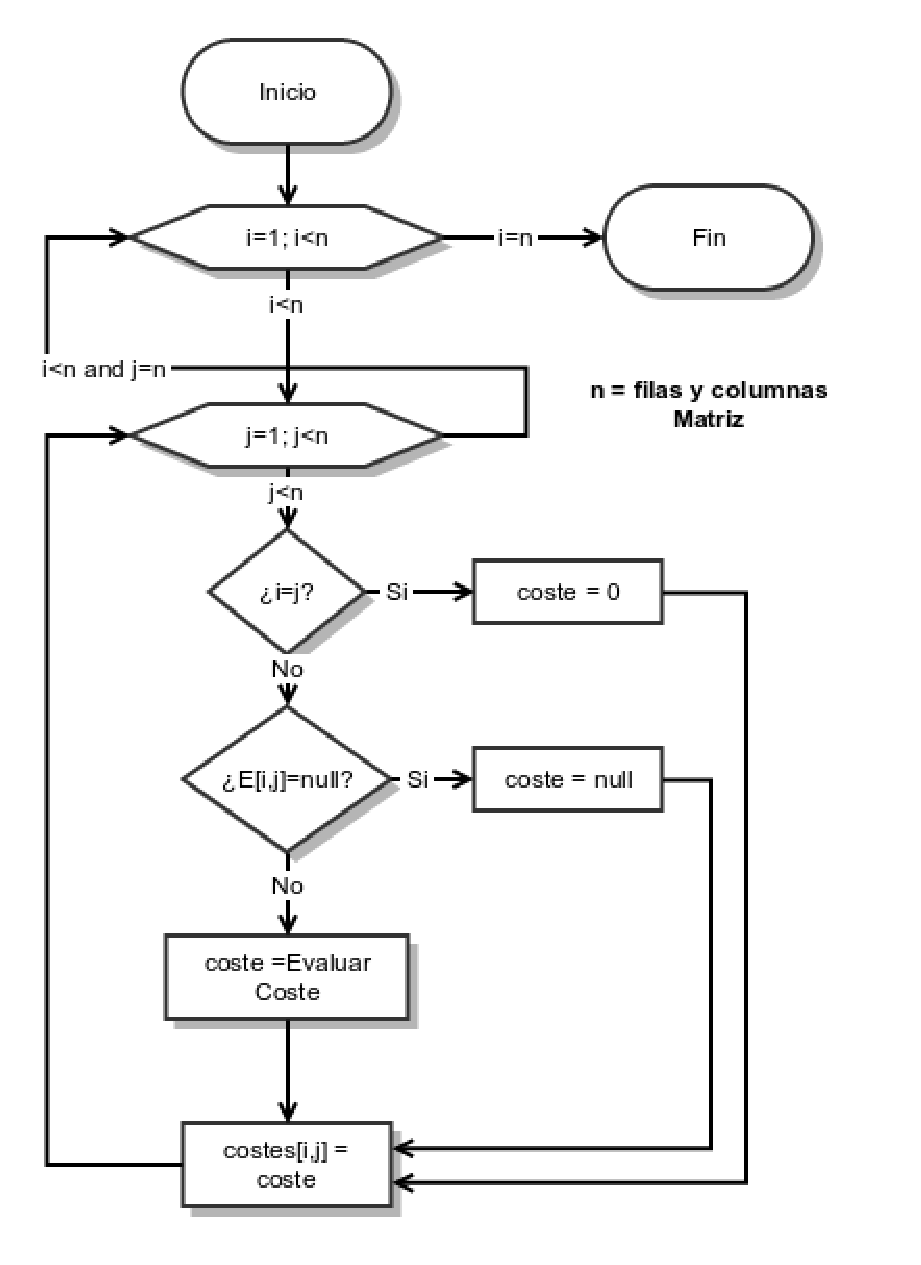
\includegraphics[scale=0.7]{./figuras/matrizCoste}
\caption{Diagrama de flujo para la construcción de matriz de costes.}\label{matrizCoste}
\end{figure}

\end{enumerate}

La asignación de los valores $\alpha_i$, $\beta_i$, $\gamma_i$ y $\sigma_i$ se ha realizado en la sección \ref{cap:evaluation}, donde a partir del estudio sobre los diferentes flujos, y resultados obtenidos, se han estimado los que consideramos mejores valores para cada tipo de tráfico ($i$). Los distintos componentes del coste han de estimarse previamente. A este paso se le ha denominado: estimación de estadísticas de red.  

%%%%%%%%%%%%%%%%%%%
\subsection{Descripción de métricas de coste}\label{funcionesEvaluacion}

Para la evaluación de costes de cada enlace se usan 4 funciones diferentes, cada una relacionada con el tipo de evaluación que realiza: función de evaluación de latencias ($C_{latency}[E]$), función de evaluación de \textit{jitter} ($C_{jitter}[E]$),función de evaluación de pérdidas de paquetes ($C_{loss}[E])$ y función de evaluación de carga (($C_{load}[E])$). 
 Estas cuatro funciones se normalizan para que devuelvan valores de coste entre 0 y 100. Una vez definidas estas funciones de coste, es necesario ajustar los pesos $\alpha$, $\beta$, $\gamma$ y $\sigma$ de cada uno de dichos componentes para obtener el coste total estimado para cada tipo de tráfico. 
 
%%%%%%%%%%%%%%%%
\subsubsection{Función de evaluación de latencias}

Gracias a la medida de latencias descrita en la sección \ref{latency} y evaluada en el apartado \ref{sec:eval-latencias}, podemos ahora realizar una evaluación del coste asociado a los enlaces en función de la latencia.  

 Hay que tener en cuenta que es necesario normalizar la función de costes para que su rango esté entre de 0 a 100. Eso implica que hay que determinar qué valores de retardo tendrán asociado el valor 0 y cuáles el 100. Ya que esta función se utiliza para comparar los costes de varios caminos en el algoritmo de encaminamiento. Por ello, se normalizará la salida de esta (y siguientes) funciones de coste teniendo en cuenta la latencia mínima  y máxima.
 
 Para este cálculo será usada la latencia media estimada por el módulo de recolección de estadísticas diseñado. La latencia mínima encontrada en la red tendrá asociado un coste de 1. También se tendrá en cuenta la latencia máxima encontrada en la red pues será necesario acotar el coste resultante entre los límites establecidos (1 y 100), siendo en este caso 100 el coste máximo.

 El cálculo asociado al resto de retardos se debe calcular teniendo en cuenta la normalización descrita. En este trabajo se han barajado dos posibilidades para calcularlas: ajuste exponencial o ajuste lineal de costes. A continuación se describe una topología sobre la que se ejemplificará el cálculo de costes mediante ambas alternativas
 
\paragraph{Topología de ejemplo.}

Se hará uso de la topología de la figura \ref{topo1} para ilustrar el cálculo de costes para latencias. En esta topología podemos visualizar 4 \emph{switches} conectados uno tras de otro, por tanto tendremos tres enlaces que evaluar. Estos enlaces se configuran para tener los siguientes retardos $l_{sw_i-sw_j}$:

\begin{center}
$l_{S1-S2} = 25 ms$ \\ $l_{S2-S3} = 500 ms$ \\ $l_{S3-S4} = 100 ms $
\end{center}

\begin{figure}[tb]
\centering
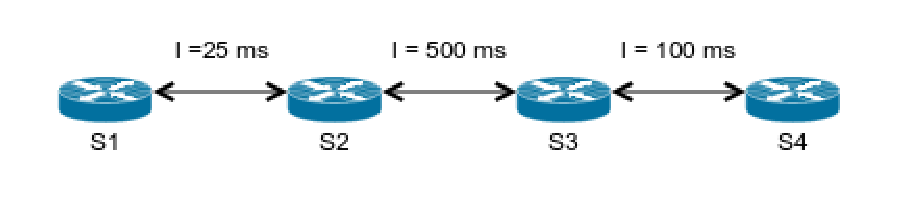
\includegraphics[scale=0.8]{./figuras/topo1}
\caption{Ejemplo de topología para el cálculo de costes asociados a latencias.}\label{topo1}
\end{figure}

En esta topología, las latencias mínimas y máximas son 25ms y 500ms respectivamente. Estos valores hay que tenerlos en cuenta, pues los costes se calcularán considerando esos valores como umbral inferior y superior, respectivamente.

\paragraph{Correspondencia entre latencias y costes.}

Para el cálculo de costes en función de la latencia se propone hacer uso de un ajuste lineal que distribuya el coste entre las latencias máximas y mínimas registradas en la red. Se puede usar otro tipo de ajuste, por ejemplo exponencial, pero por simplicidad y eficiencia nos hemos decantado por uno de tipo lineal.
 
  Para un ajuste lineal, el cálculo se lleva a cabo de la siguiente manera:
 
\begin{equation}
 C_{latencia}[E]=a + b \cdot d
 \label{ec:clatencia-lin}
\end{equation} 

 donde $d$ es la latencia estimada en el enlace y medida en milisegundos, y $a$ y $b$ deben obtenerse del siguiente sistema de ecuaciones:
 
 \begin{eqnarray}
   a \cdot d_{min} + b=1\\\nonumber
   a \cdot d_{max} + b=100
 \label{ec:clatencia-lin-sis}
\end{eqnarray} 

 Por ejemplo, para calcular el coste asociado al enlace de la topología presentada en \ref{topo1}, donde $d_{min}=25$ y $d_{max}=500$. Despejando del anterior sistema obtenemos que $a=0.208$ y $b=-4.211$. Por tanto, para el enlace S3-S4 obtenemos que $C_{latencia}[S3-S4]= -4.2 + 0.208 \cdot 100=16.6$
 
 Se debe establecer una diferencia mínima entre las latencias mínimas y máximas, a fin de limitar el impacto del coste. Por ejemplo, en una red donde todos los enlaces tengan una latencia asociada igual, una variación menor a un milisegundo podría suponer una diferencia de coste de 99 unidades, siendo en este caso una mala medida. Por tanto se establece un mínimo de diferencias que será capaz de cubrir ampliamente el aumento de latencias debidas al tiempo de procesamiento por parte del controlador. A partir de los resultados observados experimentalmente en pruebas previas, se propone usar una diferencia mínima de 5 ms.

%%%%%%%%%%%%
%
\subsubsection{Función de evaluación de \textit{jitter}.}

Uno de los problemas que más afectan a aplicaciones multimedia es el \textit{jitter}. Una de las primeras definiciones de esta propiedad se puede encontrar en \cite{berriman1996jitter}, donde se define como la variación en el tiempo en la llegada de los paquetes, causada por congestión de red, perdida de sincronización o por las diferentes rutas seguidas por los paquetes para llegar al destino. El \textit{jitter} es por tanto uno de los problemas más complicados de paliar/solucionar en redes multimedia, con lo que elegir el mejor camino (en cuanto a \textit{jitter}) en ciertos tipos de tráfico tendrá un gran valor.

La detección de \textit{jitter} se lleva a cabo usando las medidas temporales y medias de latencia analizadas en la sección \ref{latency}. Esta detección tiene ciertas complicaciones, pues como se comprobó existen variaciones que no dependen únicamente del enlace en las medidas, sino que también dependen del tiempo de procesamiento en el controlador. Otro inconveniente de estas medidas está provocada por la relación entre \textit{jitter} y latencias. Por ejemplo, un \textit{jitter} de un milisegundo en una red con latencias promedio de 10 milisegundos tendría una relevancia muy importante, sin embargo encontrarnos este mismo \textit{jitter} de un milisegundo en redes con latencias de 500 milisegundos tendrá una importancia mucho menor, sin embargo, si solo se consideran \textit{jitter} mínimo y máximo para el cálculo, se obtendrá el mismo coste para el enlace en ambos casos.

Para solucionar estos dos problemas se establece:

\begin{enumerate}
\item Limitar una diferencia mínima entre los valores máximos y mínimos de \textit{jitter}, a partir de la cual comenzar a calcular costes estándares (si la diferencia fuera menor, los enlaces tendrían un coste asociado al \textit{jitter} igual para todos).
\item Escalar el coste del \textit{jitter} en función de las latencias máximas y mínimas encontradas, de modo que un \textit{jitter} muy grande en una red de latencias pequeñas (y cercanas), será mucho más significativo en cuanto a coste que un \textit{jitter} grande en una red lenta y de grandes diferencias.
\end{enumerate}

Con estas consideraciones se ha decidido calcular el \textit{jitter} como la ecuación \ref{eq:77}:

\begin{equation}\label{eq:77}
jitter = |latencia_{instantanea} - latencia_{promedio}|
\end{equation}


Con el \textit{jitter} por enlace calculado sería el momento se conseguir el coste en función de cada enlace. Se hará un ajuste lineal del mismo tipo que se realizó en el cálculo de costes para latencias, sin embargo en este ajuste se tendrá en cuenta el factor a (pendiente) del ajuste de latencias. Este factor servirá para escalar el coste obtenido por el \textit{jitter} a valores que estén en consonancia a las latencias obtenidas en la red. 

Por ejemplo, en la topología de la figura  \ref{topologyJitter}:

\begin{figure}[tb]
\centering
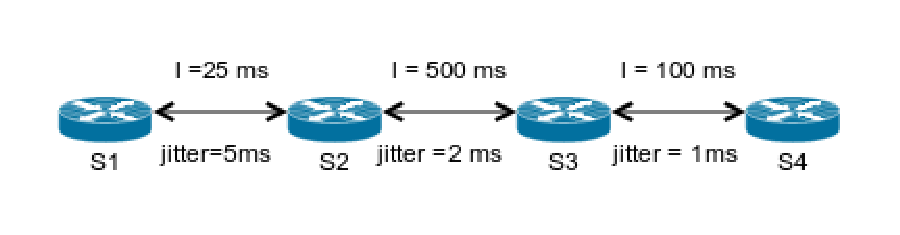
\includegraphics[scale=0.9]{./figuras/topologyJitter}
\caption{Topología para el cálculo de costes de \emph{jitter} en enlaces.}\label{topologyJitter}
\end{figure}

Siguiendo el mismo procedimiento descrito para el ajuste de latencias obtendremos los valores: $a_{jitter} = 24.75$, $b_{jitter} = -23.75$, combinados con el valor $a_{latencia}=0.208$, obtenido anteriormente, devuelven un coste asociado $C_{jitter}=5.356$  

Con este ajuste se consigue normalizar el coste asociado al \textit{jitter} en función de las latencias encontradas en la red. El coste asociado al \textit{jitter} no estará acotado entre 1 y 100 al depender de la pendiente de la recta de ajuste para latencias, pero siempre mantendrá un valor relacionado al estado de la red.

%%%%%%%%%%%%%
\subsubsection{Función de evaluación de pérdidas.} 

Para poder evaluar las pérdidas en la red, se usará el porcentaje de estas en un enlace. Este porcentaje equivaldrá al coste de forma directa, con lo que estará limitado entre 0 y 100. Para obtener el valor asociado al porcentaje de pérdidas se hará uso de las estadísticas recogidas en la sección \ref{sub:estadisticas1}, y se usará la ecuación \ref{eq:79}\footnote{Se usarán los bytes enviados o recibidos según la orientación del enlace. Por ejemplo para el enlace 2-1 se usarán los bytes enviados por el puerto correspondiente al enlace S2-S1 en el nodo 2, y los recibidos por el puerto correspondiente a dicho enlace en el nodo 1.}.

\begin{equation}\label{eq:79}
C_{loss}(E) = \frac{sentBytes(E) - receivedBytes(E)}{sentBytes(E)} \cdot 100
\end{equation}

\subsubsection{Función de evaluación de carga.}\label{sub:funcioncarga}

Esta es una de las funciones más difíciles de ponderar y describir ya que no tenemos medidas sobre el ancho de banda disponible en un enlace, y tan solo podremos estimar el ancho de banda consumido por este. De este modo no podemos garantizar asociar un mayor coste a un enlace con menor ancho de banda disponible, sino que asociaremos el mayor coste al enlace con mayor uso en la red. \footnote{En la implementación final no se usa este coste al no garantizar medidas ``útiles"}.

Para evaluar la carga se ha añadido al procesado de estadísticas una medida de tiempo que permita un cálculo de ancho de banda consumido. Se hace uso de la ecuación \ref{eq:710}.

\begin{equation}\label{eq:710}
BW(E) = \frac{sentBytest1(E)-sentBytest0(E)}{t1-t0}
\end{equation}

Esta ecuación devuelve unos valores estimados en Bps. Estos valores se deberán transformar a una medida más acorde a las velocidades de transmisión actuales (MBps). A partir del ancho de banda consumido se realizará un ajuste linea como los realizados para las funciones anteriores (con costes mínimo 1 y máximo 100), que permita distribuir el coste asociado al ancho de banda. 

Ya que no se ha implementado en la solución final, el coeficiente $\sigma_i$ tiene asignado el valor fijo 0.


%%%%%%%%%%%%%%%%%%%%%%%%%%
%
%
%
\section{Estimación de estadísticas de red}
\label{sec:parametros-calidad-servicio}

 El controlador \emph{OpenDayLight} cuenta en su núcleo con un recolector de estadísticas que almacena información sobre todos los elementos de red susceptibles de contar con estadísticas de red (paquetes enviados por un puerto, bytes recibidos por un \textit{switch}, paquetes que han coincidido con un flujo en un \textit{switch}, etc.), \cite{developerGuide}. Haciendo uso de este almacén de estadísticas conseguiremos obtener datos que se usarán para la construcción de los costes asociados a cada enlace. En la figura \ref{statisticsODL} se puede ver dónde se implementa en \emph{OpenDayLight} el módulo de gestión de estadísticas, que puede ser consultado desde las aplicaciones de red que se desarrollen.

%%%%%%%%%%%%%%%%%%
\begin{figure}[tb]
\centering
\hspace*{-0.3cm}
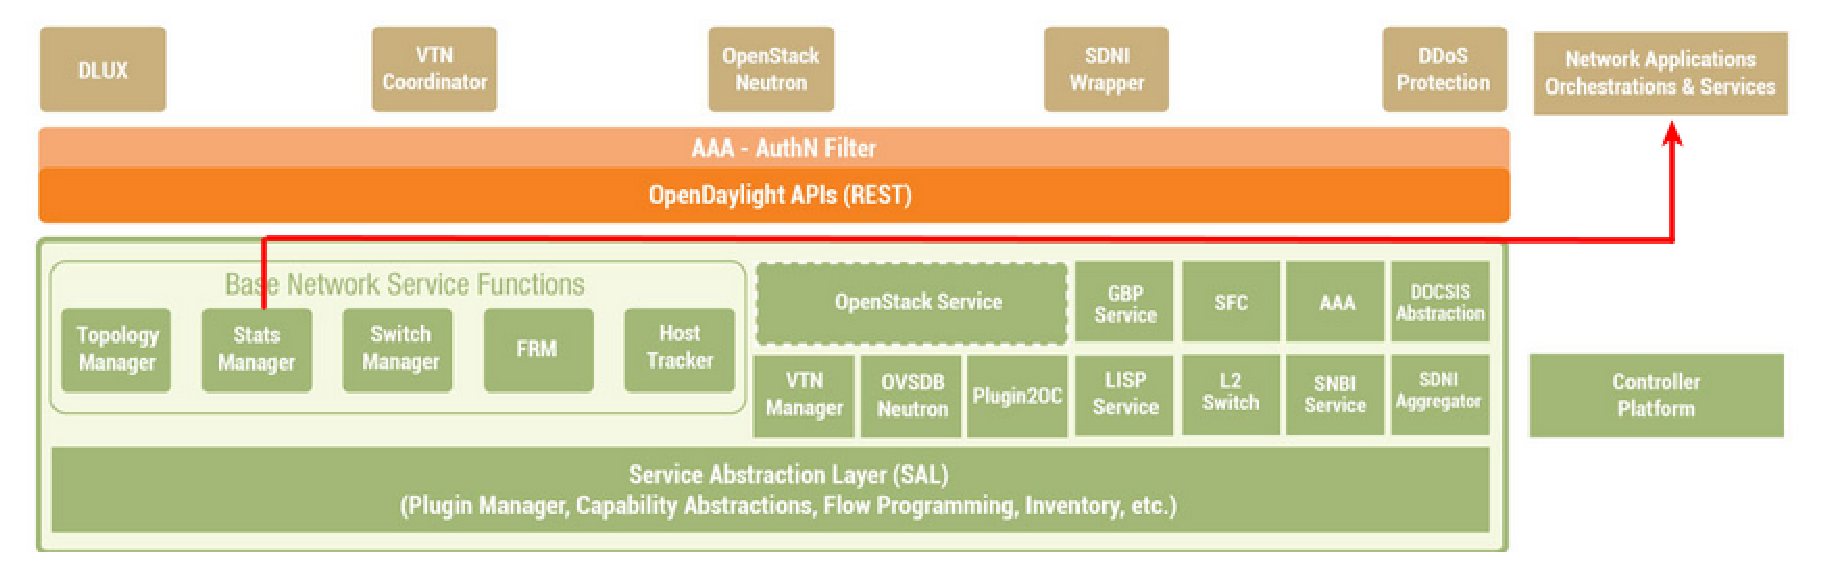
\includegraphics[scale=0.55]{./figuras/statisticsODL}
\caption[Módulo estadístico núcleo ODL.]{Obtención de estadísticas del módulo situado en el núcleo de ODL.}\label{statisticsODL}
\end{figure}
%%%%%%%%%%%%%%%%%%

 Sin embargo, hay algunas estadísticas que, aunque teóricamente deberían estar disponibles en el controlador \emph{OpenDayLight}, en la práctica no es así, por lo que nuestra solución ha tenido que implementarlas.   
En el desarrollo se ha hecho uso de tres estadísticas principales (de entre todas las posibles). A continuación se detalla la estrategia de obtención de dichos parámetros.

%%%%%%%%%%%%%%%%%%%%%%%%%%%%%%%%%%%%%
%
\subsection{Latencia y \textit{jitter}} \label{latency}

 Uno de los parámetros que puede tener impacto en las aplicaciones interactivas de red es la \emph{latencia} extremo a extremo. Es decir, el tiempo que transcurre desde que un paquete es enviado hasta que llega al destino.
 En esa latencia influyen los retardos que se producen en cada \emph{switch} y cada enlace. En este apartado se describe cómo se calculan los retardos por enlace en nuestra solución.
 
 La latencia como tal no es una medida estadística que se haya obtenido a partir del módulo \ac{ODL}, sino que se ha obtenido a partir de diversas medidas de retardos de paquetes. Como tal existe una propiedad en los enlaces (recogida dentro de las propiedades de los enlaces en redes \ac{SDN}) que es la llamada \emph{Latency}. Sin embargo al intentar extraer esta propiedad mediante los métodos proporcionados en la \ac{API} de JAVA, no se ha obtenido valor alguno, con lo que, siendo una medida necesaria para evaluación de costes, se ha optado por medir nuestras propias estadísticas temporales. Se espera que este inconveniente se solucione en versiones futuras del controlador que implementen estas estadísticas de forma nativa.

Para la medida de estadísticas (no solo las de latencia), es necesario añadir un proceso de aprendizaje por el cual se almacenan valores estadísticos para todos los enlaces disponibles durante un periodo de entrenamiento inicial. La duración de este periodo de aprendizaje se ha definido en el capítulo \ref{cap:evaluation} a partir de los experimentos. De este modo se establece un período de tiempo (paquetes) durante el cual todos los enlaces transmiten paquetes y se almacenan las estadísticas correspondientes a cada enlace. El proceso seguido para la obtención de estadísticas de retardos es el que se enumera a continuación:
 
\begin{enumerate}
\item Durante la fase de entrenamiento en la que se obtienen las estadísticas de retardos, los \emph{switches} reenvían cada paquete al controlador. Si en el controlador se identifica como un tipo de flujo de los considerados en la solución (\ac{ICMP}, Vídeo, Voz o \ac{TCP}), se almacena junto a una marca temporal e información del puerto de entrada justo a su llegada. También se incluye una marca de tiempo a su salida del \emph{switch}. 

\item El controlador conoce qué enlaces existen. En la información de los enlaces se incluyen los identificadores de los puertos y \emph{switches} que conectan. Si cuando llega un paquete $i$ al controlador se comprueba que existe una marca de tiempo asociado al paquete y al enlace por el que entra al \emph{switch}, se calcula la diferencia entre el instante de tiempo en el que se envió por el puerto de salida ($t_{i,out}$) y el tiempo en el que se recibe por el puerto de entrada ($t_{i,in}$).  A continuación, el paquete almacenado se elimina de la memoria del controlador. En caso de no estar almacenado se continua el procesamiento normal y a la salida (cuando es enviado por algún puerto), se almacena junto a la marca temporal $t_{i,out}$.

Por cada paquete $i$, estas medidas de latencia se estiman de acuerdo a la ecuación \ref{eq:51}:

\begin{equation}\label{eq:51}
latency_i = t_{i,in} - t_{i,out}
\end{equation}

\item Una vez calculada la diferencia temporal, estos datos son enviados a una función que los inserta en dos matrices que serán las que posteriormente se usen para la evaluación de costes. Una matriz contiene la media de los últimos valores de latencia para cada enlace, mientras que la otra solo contiene el último valor. El número de valores para el cálculo de la media se ha definido en el capítulo \ref{cap:evaluation}.

\end{enumerate}

El diagrama de flujo de la figura \ref{packetTime} muestra el proceso explicado anteriormente.

\begin{figure}[tb]
\centering
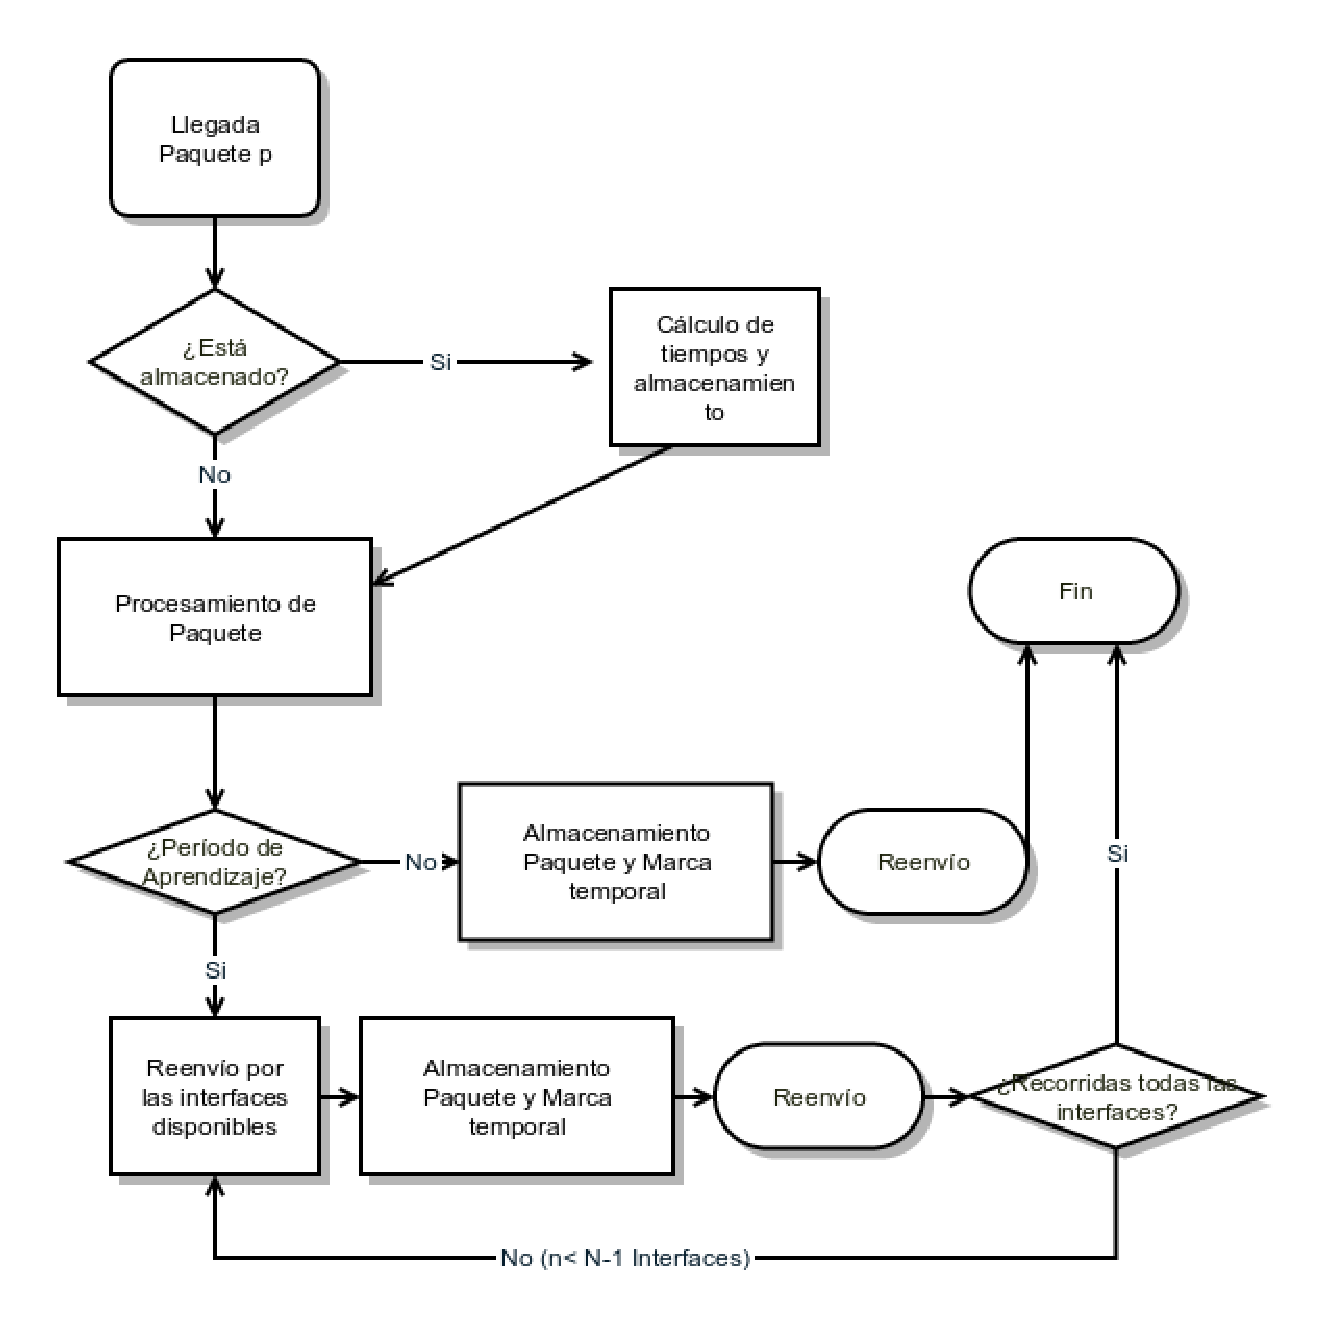
\includegraphics[scale=0.5]{./figuras/packettimeflow}
\caption[Procesamiento de paquetes para la obtención de latencias.]{Diagrama de flujo del procesamiento de paquetes para la obtención de latencias en enlaces.}\label{packetTime}
\end{figure}

Nótese que mediante este procedimiento se obtiene una medida experimental, lo que no es exactamente la latencia de un enlace, como se muestra en las figuras \ref{medirPaquete} y \ref{medirPaquete2}. El tiempo medido que nuestra solución obtiene es igual al de la ecuación \ref{eq:52}. Para conseguir resultados más exactos, el procedimiento intenta no contabilizar el retardo de procesamiento dentro del controlador.

% \vspace*{0.2cm}
\begin{equation}
latency'_i = t_{C-1} + t_{1-2} + t_{2-C}
\label{eq:52}
\end{equation}

Donde $t_{C-1}$ es la latencia sufrida por un paquete para ir desde el nodo 1 al controlador. $t_{1-2}$ corresponde a la latencia sufrida por un paquete para ser transmitido a través del enlace entre S1 y S2. Por último, $t_{2-C}$ es el retardo experimentado por un paquete para ir desde el controlador hacia el nodo 2.

En la sección \ref{sec:eval-latencias} se estiman los retardos adicionales a la latencia como tal. Sin embargo es preciso remarcar que estos tiempos afectarán por igual a todos los enlaces (suponemos que todos los nodos están conectados al controlador con enlaces de iguales características), con lo que la variación respecto a los cálculos que se realizaran con la latencia ideal, debe ser mínima. 

\begin{figure}[tb]
\centering
\hspace*{-1cm}
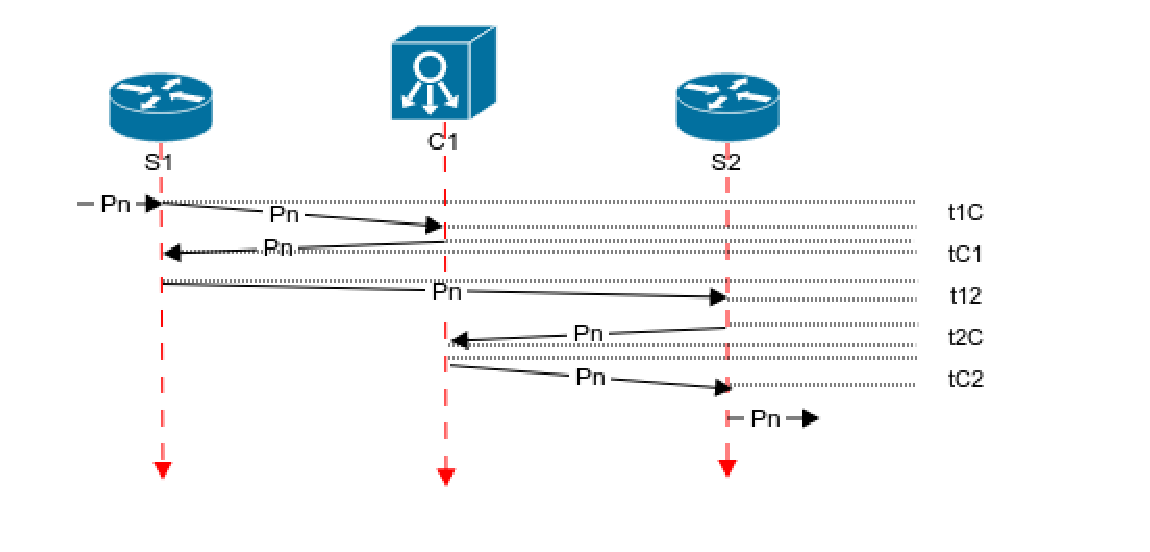
\includegraphics[scale=1]{./figuras/medirPaquete}
\caption[Exposición de tiempos para la medida de latencias.]{Intercambio de paquetes durante la medida de latencias.}\label{medirPaquete}
\end{figure}

\begin{figure}[tb]
\centering
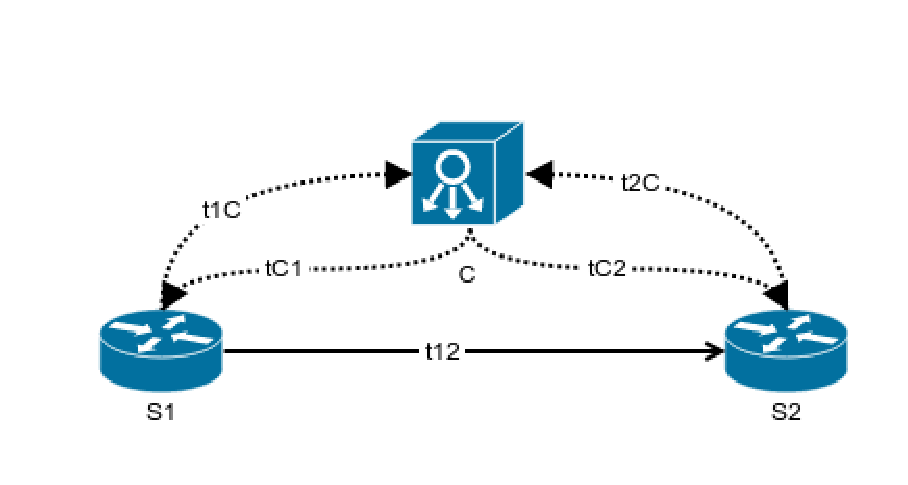
\includegraphics[scale=0.8]{./figuras/medirPaquete2}
\caption[Exposición de tiempos para la medida de latencias.]{Intercambio de paquetes durante la medida de latencias.}\label{medirPaquete2}
\end{figure}

Como se ha comentado anteriormente, estas medidas serán ponderadas en la función de evaluación del coste por enlace en función del tipo de tráfico.

%%%%%%%%%%%%%%%%%%
%
\subsection{Pérdidas de paquetes}

La recogida de estadísticas para pérdidas (y cualquier estadística relacionada con peticiones al módulo \textit{statisticsManager}) se hará de forma periódica de acuerdo a un tiempo establecido $t_{update}$. El valor apropiado de $t_{update}$ se estudiará con más detenimiento en la sección sobre actualización de la topología. Las pérdidas se representarán mediante un porcentaje, calculado como se explica a continuación.

Cada vez que se cumple el período de actualización $t_{update}$ establecido, se consulta cuántos paquetes han sido enviados y recibidos por cada uno de los dos \emph{NodeConnector} en cada enlace. Tenga en cuenta que un enlace tiene un \textit{TailConnector} y un \textit{HeadConnector}. Por ejemplo, el enlace 1-2 tendrá como \textit{HeadConnector} un \textit{Connector} del nodo 2, y como \textit{TailConnector} un \textit{Connector} del nodo 1. 
Una vez recogidas las estadísticas, se almacenan en un mapa de enlaces que posteriormente será usado por los diferentes manejadores para la estimación de costes asociados. Cada enlace tendrá asociado por tanto un mapa donde se habrán almacenado las diferentes estadísticas (en este caso especialmente interesantes la cantidad de paquetes y bytes enviados por el \textit{TailConnector} y los recibidos por el \textit{HeadConnector} para la estimación del porcentaje de pérdidas).

Cada vez que se cumple el período de actualización, se lleva a cabo esta actualización de estadísticas y se pasa a los manejadores correspondientes (clases para procesar cada tipo de flujo) toda la información actualizada en forma de "matriz de mapas", donde se tiene un mapa de estadísticas para cada enlace. Posteriormente, estos datos son procesados de acuerdo a la necesidad de cada tipo de flujo y manejador.

%%%%%%%%%%%%%%%%%%%%%%%%%%%
\subsection{Carga en los enlaces}
La carga en los enlaces se define como el ancho de banda transportado por éstos. Esta se obtiene a partir de los mismos datos recogidos para la estimación de pérdidas, es decir, la cantidad de bytes y paquetes enviados y recibidos por cada puerto de cada \emph{switch}. Además de los datos estadísticos, se hace uso de un mapa que contiene los valores máximos y mínimos de cada estadística. Por ejemplo, se almacena el máximo número de paquetes enviados por un \textit{connector}. De este modo podemos estimar la carga soportada por un enlace y paliar la falta de información referente a la capacidad de los enlaces (que esperamos incluya las próximas versiones del controlador).

Con estos datos y estadísticas se construirá posteriormente la matriz de costes asociada a cada tipo de flujo y que permitirá un encaminamiento óptimo por tipo de flujo.

%%%%%%%%%%%%%%%%%%%%%%%%%%%%%%
%
%
\section{Configuración de las rutas en los \emph{switches}}

Haciendo uso del algoritmo \textit{Dijkstra} somos capaces de obtener el mejor camino entre dos nodos, de acuerdo a la métrica que elijamos. Los flujos que coincidan con nuestras especificaciones deberán seguir el camino precalculado. Las redes con \emph{switches OpenFlow} implican la necesidad de instalar una regla por cada flujo en los nodos que componen el camino. En nuestra solución, esto se llevará a cabo de acuerdo a los pasos descritos a continuación, y plasmados en la figura \ref{installFlow}.

\begin{enumerate}
\item Localización de los extremos.
La \ac{API} usada para el desarrollo provee métodos que nos permiten obtener los nodos a los cuales están conectados los \textit{hosts}. Estos métodos devuelven un mapa donde cada \textit{host\footnote{Cada \emph{host} tendrá asociada su dirección \ac{IP}}}. Gracias a la \ac{IP} destino y origen, obtendremos los nodos en los que estamos interesados.

\item Obtención del camino. Con los nodos origen y destino consultaremos el mapa de caminos (caminos que ya han sido calculados y almacenados). En caso de estar el camino guardado ya, pasamos al punto 4. Si el camino no está guardado, haciendo uso del \textit{Dijkstra} implementado, calcularemos el mejor camino entre los dos nodos.

\item Reordenación de camino. Uno de los problemas que se ha detectado es que a veces el algoritmo devuelve el camino sin ordenar, por ejemplo, para ir del nodo 1 al 4 nos puede devolver la sucesión de nodos: 1-2, 3-2, 4-3. Por ello se ha diseñado un procedimiento para reordenar los enlaces de las rutas.  La reordenación de caminos sigue el flujo del diagrama presentado en la figura \ref{reordenating}. A partir de esta lógica se obtiene la secuencia de nodos consecutivos, lo que posibilita la instalación de flujos. 

\begin{figure}[tb]
\centering
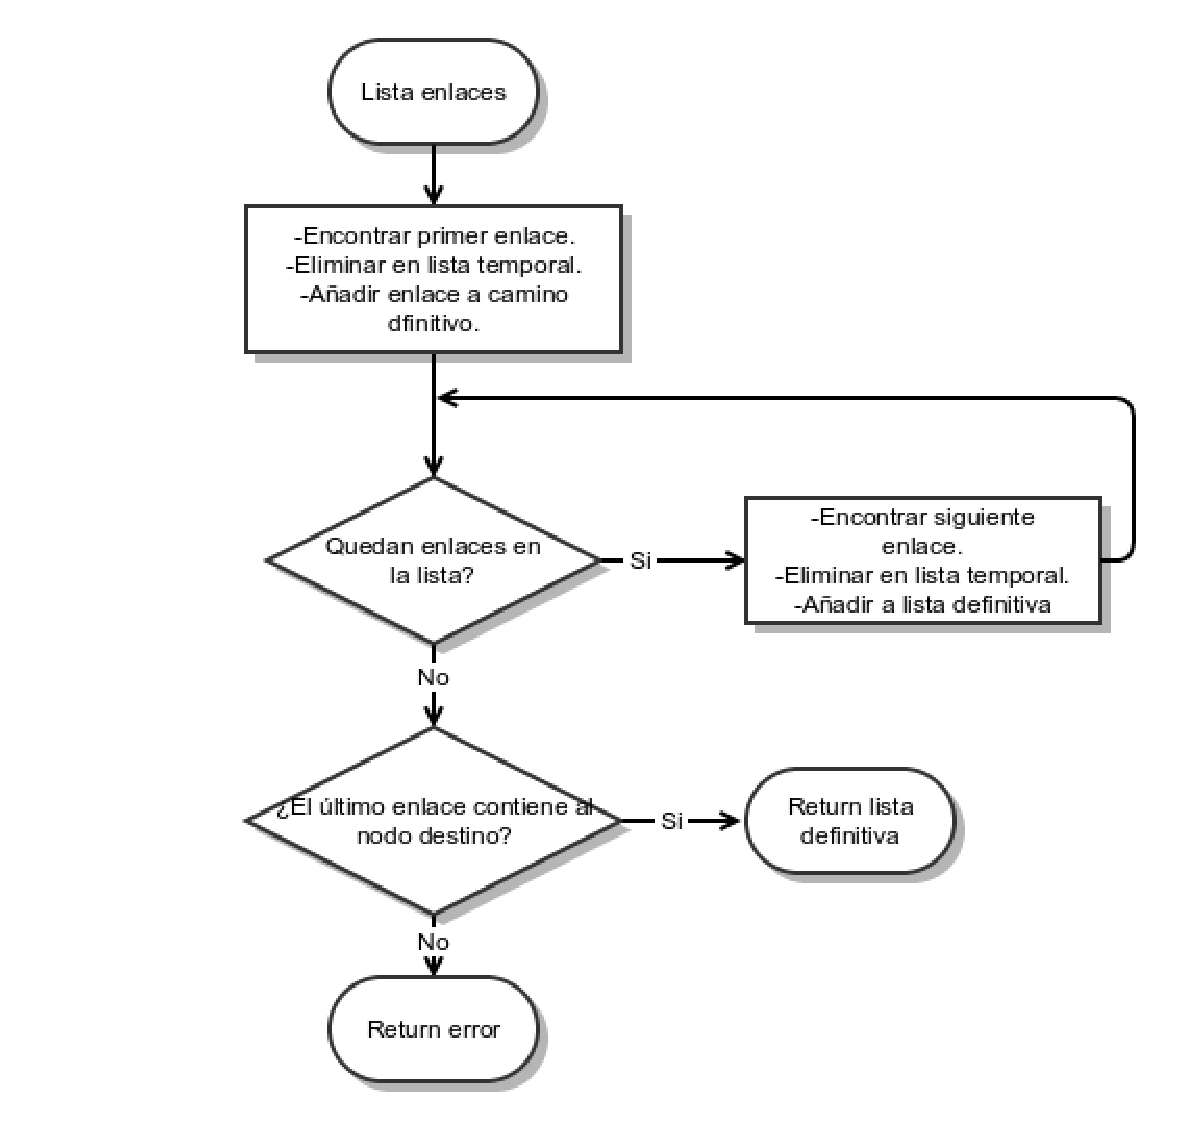
\includegraphics[scale=0.7]{./figuras/reordenating}
\caption{Diagrama de flujo para la reordenación de caminos.}
\label{reordenating}
\end{figure}

La reordenación de caminos se ha diseñado de una forma muy esquemática.

\begin{enumerate}
\item Se busca el primer nodo del camino. Buscaremos el primer nodo del camino (nodo origen) en el camino devuelto por \emph{Dijkstra}, una vez encontrado el nodo, añadiremos el enlace asociado al camino definitivo y lo eliminaremos de la lista devuelta por \emph{Dijkstra}.
\item Mientras queden enlaces en la lista, buscaremos aquellos cuyo \emph{connector} de cola, coincida con el \emph{connector} de cabecera del enlace anterior. En caso de no encontrar ningún enlace con dichas características se descarta el procedimiento y se devuelve un camino vacío.
\item Por último, una vez no quedan enlaces en la lista devuelta por \emph{Dijkstra}, se comprueba que el último enlace contiene el \emph{connector} correspondiente al nodo destino. En caso afirmativo el camino definitivo estará completo. Si esta última condición no se cumpliese devolveríamos un camino vacío.
\end{enumerate}

\item Instalación de flujos en los extremos. Una vez tenemos el camino ordenado, procedemos a instalar flujos para los extremos, es decir, instalaremos reglas de flujo para los nodos que conectan a los \textit{hosts} implicados (direcciones \ac{IP}).

\item Instalación de flujos en los nodos del camino. Se recorrerá el camino obtenido y se instalarán flujos en los nodos que reenviarán paquetes por el camino. Los flujos instalados dependerán del tipo de flujo, pues los parámetros que afectan al \textit{match}, así como las acciones varían entre tipos de tráfico.

Los flujos son instalados por orden y en el mismo proceso. Se planteó la instalación de flujos por separado (cada vez que un nodo lo pidiera), pero se concluyó que este es el método más rápido ya que existe un menor intercambio de mensajes y menor carga para la red.

\end{enumerate}

\begin{figure}[tb]
\centering

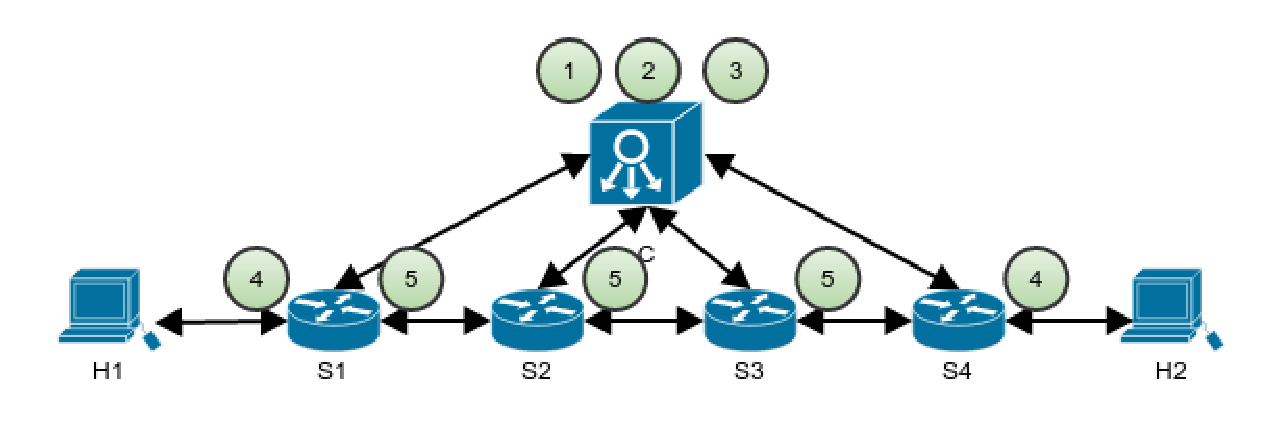
\includegraphics[scale=0.8]{./figuras/installFlow}
\caption{Proceso de instalación de flujos a lo largo de un camino.}\label{installFlow}
\end{figure}
%%%%%%%%%%%%%%%%%%%%%%%%%
%
%
\section{Actualización de topología}
\label{updateTopology}

En esta sección se describe el proceso que consigue responder ante cambios en la red tales como caídas de enlaces o nodos. Es uno de los pilares en los cuales se apoya todo el proceso para proveer de \ac{QoE} y \ac{QoS} a las aplicaciones que usan los usuarios. Para conseguir el objetivo, el procedimiento diseñado se divide en dos fases: detección y actualización de rutas.

\subsection{Detección de cambios en la topología}

Mediante el procedimiento de detección de cambios de la topología de red, nuestra solución es capaz de lanzar el procedimiento que actualice la información sobre la red, y recalcular las rutas que sean necesarias. Estos cambios comprenden la modificación de las características de los enlaces, la caída de nodos, etc. Si bien el propio controlador \emph{OpenDayLight} puede detectar los cambios en la topología (existe un módulo capaz de avisar a las aplicaciones de red de cambios en la topología), se decidió prescindir de esta posibilidad, ya que nuestro diseño contempla el tratamiento de los flujos en el mismo módulo donde se reciben los paquetes.

La detección se lleva a cabo mediante consultas sucesivas al estado de la red. El tiempo entre consultas es el mismo tiempo que el de actualización de estadísticas, $t_{update}$. El valor de este tiempo de actualización se propone como 100 ms, pudiendo ser modificado según las necesidades de red o usuario. La propuesta está basada en:

\begin{itemize}
\item [•] Un período de 100 ms garantiza la comprobación en un tiempo menor al que se tarda en actualizar todos los enlaces (como se comprobará en el capítulo \ref{cap:evaluation}.
\item [•] No se pretende sobrecargar el controlador eligiendo un tiempo menor, puesto que podría darse una situación en la cual se están actualizando estadísticas, mientras se detectan cambios en la topología, provocando dos accesos a un dato al mismo tiempo. Suponemos que con esta elección de tiempos se asegura que el tiempo de procesamiento es mucho menor a la actualización, evitando posibles problemas.
\end{itemize}

Por supuesto este valor podrá ser modificado en cualquier momento.

Desde la parte de detección es donde se detecta cuándo y dónde se produce el cambio. Tras la detección se llama a la función que manejará este cambio. La detección sigue el flujo de presentado en la figura \ref{detection}.

%%%%%%%%%%%
\begin{figure}[tb]
\centering
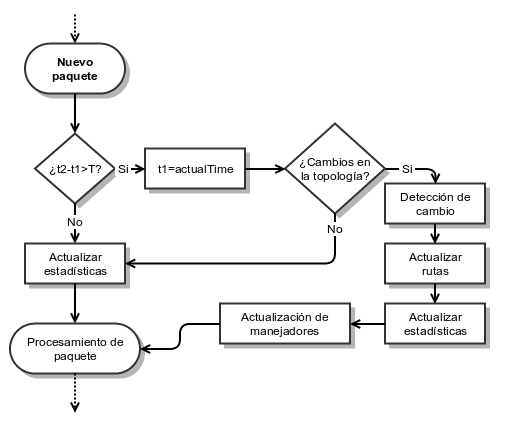
\includegraphics[scale=0.8]{./figuras/detection}
\caption{Diagrama de flujo para la detección de cambios en topología.}\label{detection}
\end{figure}
%%%%%%%%%


%%%%
%
\subsection{Actualización de rutas}

 Cada vez que es detectado un cambio en la topología se llama al procedimiento de actualización de rutas. Dentro de la actualización podríamos tener dos caminos que seguir. Por un lado se podría intentar actualizar cada ruta dando un camino alternativo para los flujos, y por otro se podría simplemente eliminar las rutas afectadas. Se ha optado por la segunda solución por dos razones: no conservar flujos que llevan tiempo sin usarse y es posible que no se vuelvan a usar. La segunda razón esta relacionada con la eficiencia de la solución, pues la carga que supondría tener que procesar eliminar flujos afectados y creación de nuevos, podría suponer una pérdida de paquetes importante. Aún así esta última tesis no se ha comprobado pues suponía una carga de trabajo muy elevada junto a la programación de la segunda solución. No por ello deja de ser una razón adecuada para la elección de la segunda solución. 

De la solución elegida surgen las tres variantes que se comparan en la tabla \ref{soluciones}:

\begin{table}[tb]
\resizebox{16cm}{!} {
\begin{tabular}{|c|c|c|c|}
\hline
{\bf Capacidad/Solución}                                                   & {\bf \begin{tabular}[c]{@{}c@{}}Borrado completo\\ de flujos\end{tabular}}                                                   & {\bf \begin{tabular}[c]{@{}c@{}}Borrado completo \\ de camino afectado\end{tabular}}                                                            & {\bf \begin{tabular}[c]{@{}c@{}}Borrado por tipo de flujo\\ de camino afectado\end{tabular}}                                                     \\ \hline
{\bf Rapidez}                                                              & \begin{tabular}[c]{@{}c@{}}Muy rápido. Solo recorre los nodos\\ y elimina flujos.\end{tabular}                               & \begin{tabular}[c]{@{}c@{}}Medio. Recorre los nodos afectados\\ y elimina todos los flujos. Consulta\\ todos los tipos de tráfico.\end{tabular} & \begin{tabular}[c]{@{}c@{}}Baja. Recorre los nodos afectados\\ y elimina los flujos afectados.\\ Necesidad de comprobar cada flujo.\end{tabular} \\ \hline
{\bf Eficiencia}                                                           & \begin{tabular}[c]{@{}c@{}}Baja. Elimina flujos \\ que no están afectados.\end{tabular}                                      & \begin{tabular}[c]{@{}c@{}}Media/Baja. Puede eliminar flujos\\ que no están afectados.\end{tabular}                                             & Alta. Sólo elimina flujos afectados.                                                                                                             \\ \hline
{\bf \begin{tabular}[c]{@{}c@{}}Facilidad de \\ programación\end{tabular}} & Muy sencillo.                                                                                                                & Media.                                                                                                                                          & \begin{tabular}[c]{@{}c@{}}Difícil. Necesidad de comprobar\\ cada flujo por cada tráfico.\end{tabular}                                           \\ \hline
{\bf Funcionalidad}                                                        & \begin{tabular}[c]{@{}c@{}}Imposible de usar. Error con \\ función para eliminar todos los\\ flujos de un nodo.\end{tabular} & \begin{tabular}[c]{@{}c@{}}Imposible de usar. Error con función \\ para eliminar todos los\\ flujos de un nodo.\end{tabular}                    &                                                                                                                                                 \begin{tabular}[c]{@{}c@{}}Completa. Elimina los flujos\\ afectados.\end{tabular} \\ \hline
\end{tabular}
}
\caption{Comparativa soluciones propuestas para actualización de ruta.}\label{soluciones}
\end{table}

Como se extrae de la tabla \ref{soluciones} se debe escoger la solución 3, borrado por tipo de flujo afectado, ya que es la de mayor eficiencia en cuanto a conservar flujos útiles e implica una comunicación menor con \emph{switches}, evitando retardos provocados por la comunicación del controlador con estos. El resto de soluciones se intentaron usar para hacer una comparativa de resultados, pero en la versión actual del controlador ha sido imposible usarlas.

La solución elegida está descrita a continuación, además se puede consultar el diagrama de flujo en la imagen \ref{updateTopology}.

\begin{enumerate}
\item Se recibe el enlace que ha cambiado según la detección (cuando un nodo cae, todos sus enlaces son detectados y pasan por este proceso de forma individual).
\item Por orden se buscan caminos afectados por cada uno de los 4 tipos de tráfico afectados.
\item Por cada tipo de tráfico:
\begin{enumerate}
\item Se comprueba si existen caminos afectados.
\item En caso positivo se recorren los nodos del camino (suponemos estos caminos ordenados, al haber sido almacenados tras una reordenación).
\item En cada nodo se comprueban los flujos instalados buscando flujos coincidentes con los que se deben eliminar. Por cada flujo se comprueba si su acción de envío coincide con el enlace que corresponda del camino. Se podría intentar eliminar solo el enlace afectado, pero en ese caso surgen problemas con el cálculo de caminos extremo a extremo al haber flujos instalados ya.
\end{enumerate}
\item Finalmente se devuelve el control al programa de detección que actualizará mapas y estadísticas de de los manejadores.
\end{enumerate}

Se da por terminado este capítulo donde se ha descrito cada uno de los elementos que posteriormente implementaremos en el sistema para poder alcanzar los objetivos del proyecto.

\begin{figure}[tb]
\centering
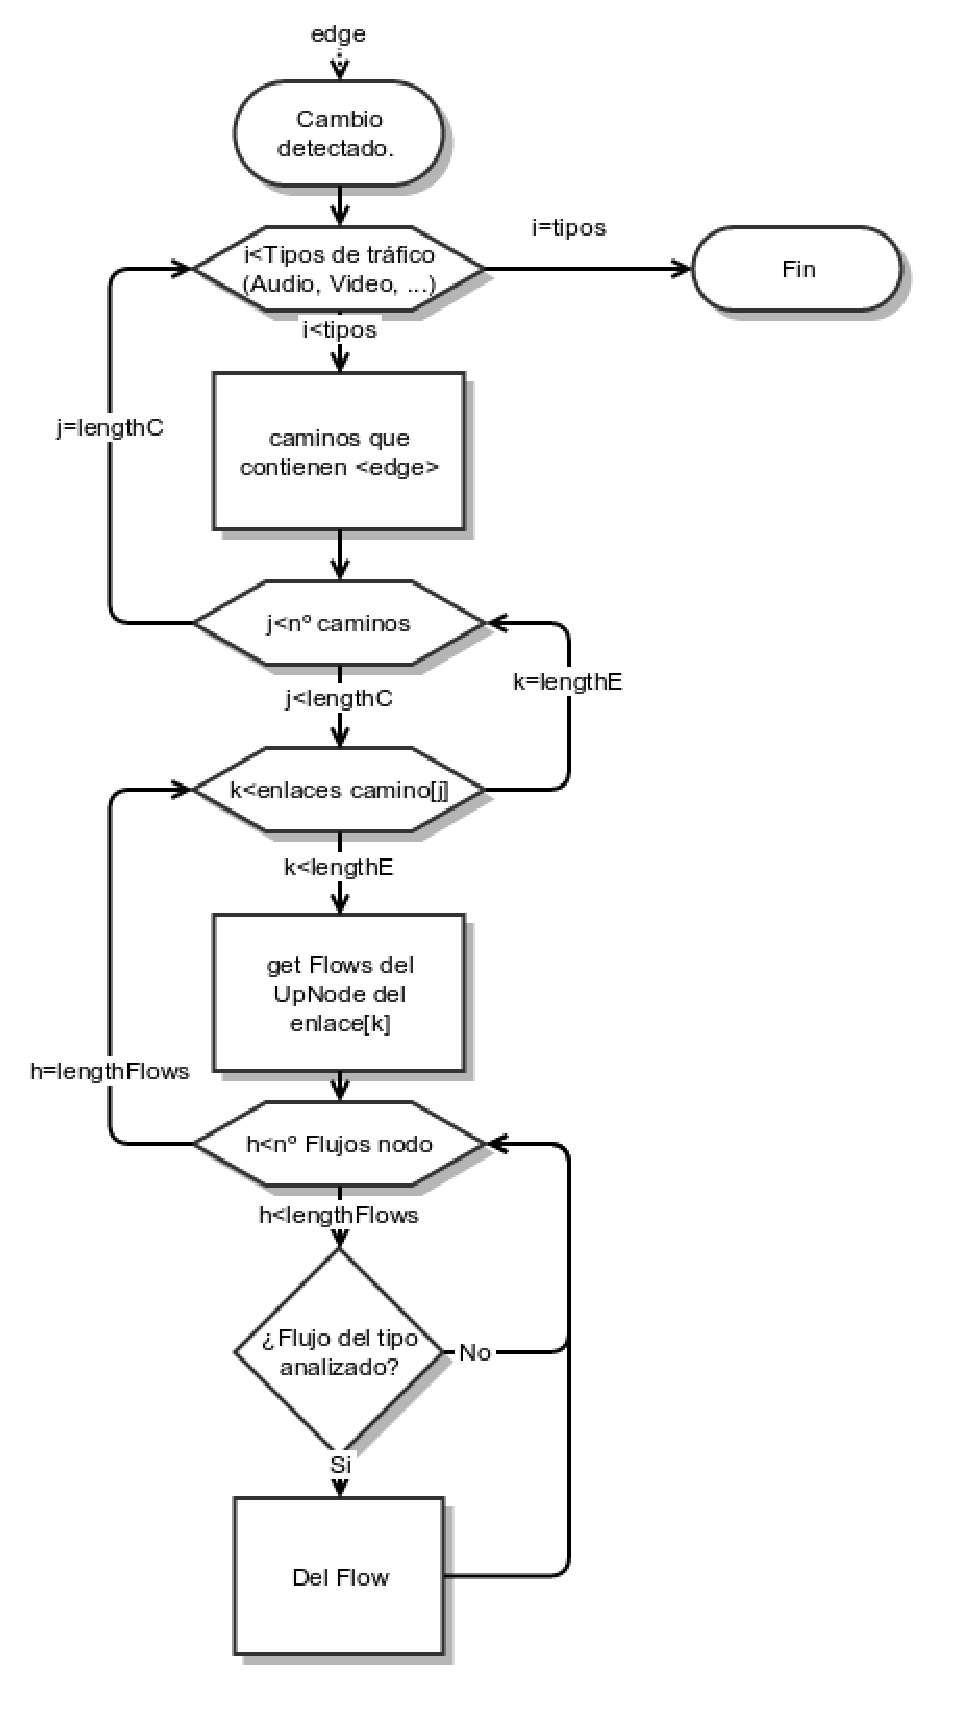
\includegraphics[scale=0.7]{./figuras/updateTopology}
\caption{Diagrama de flujo del proceso de actualización de topología}\label{updateTopology}
\end{figure}

\chapter{Entorno de desarrollo}
\label{desarrollo}
 
A lo largo de este capítulo se pretende introducir todos los elementos que formarán y permitirán la ejecución final de la solución propuesta. Comenzaremos describiendo el entorno en el cual se ejecutará dicha solución. Continuaremos describiendo la herramienta que posibilita que en un solo equipo puedan ser emuladas redes de gran complejidad, mininet. Al ser una parte troncal de este trabajo dedicaremos un apartado completo a la aplicación. Por último se tratará el entorno de ejecución de \emph{OpenDayLight}, así como las herramientas que permiten desarrollar y ejecutar aplicaciones para este controlador.

\section{Entorno de ejecución}
Para agilizar el desarrollo, la ejecución y las pruebas del sistema desarrollado, se ha optado por integrar todos los elementos del entorno en un sólo equipo informático. Dicho equipo deberá cumplir ciertas condiciones. La de mayor importancia es que se trate de un equipo con \ac{SO} Línux (Ubuntu \cite{ubuntu} y experimentalmente Fedora \cite{fedora}), o que el \ac{SO} nativo sea capaz de ejecutar alguno de los sistemas permitidos (mediante el uso de virtualización). Esta condición viene impuesta por el modelo de \textit{switch} \ac{SDN} elegido, \textit{Open vSwitch}, soportado por las versiones más recientes de Ubuntu (a partir de la 12.04) y a partir de la versión 20 por \textit{F}edora.

\subsection{Comparativa}
Existen dos \ac{SO} sobre los cuales podremos desarrollar y ejecutar el sistema de forma nativa. A continuación se comparán las dos posibilidades existenetes, para finalmente tomar una decisión.

De los sistemas basados en Línux, Ubuntu y \textit{F}edora son dos de los más populares actualmente. La colaboración por parte de la comunidad en ambos casos, y tener dos grandes compañías (\textit{C}anonical y Red Hat respectivamente) como soporte, han hecho que sean alternativas para los \ac{SO} tradicionales para usuarios. Una de las ventajas principales de Ubuntu (para casos específicos como el de este trabajo) es la estabilidad de software. Esta ventaja radica en la mentalidad de los desarrolladores: mientras que en \textit{F}edora se prima la innovación y la mejora continua, \textit{C}anonical prefiere seguir un camino más estable y de menor desarrollo, a fin de introducir mejoras testadas exhaustivamente. Para un desarrollo a largo plazo se prefiere un \ac{SO} estable. 

Otra de las razones que pesarán en la decisión es el apoyo de la comunidad. Contando los dos sistemas con un gran número de usuarios activos y desarrolladores, el sistema mantenido por \textit{C}anonical, tradicionalmente (y actualmente) cuenta con una comunidad mayor, con lo que enfrentarse a cualquier problema con el sistema tendrá una mayor probabilidad de éxito de ser resuelto.

Por último se ha de destacar que el emulador de redes que se usará, mininet \cite{mininet}, está perfectamente integrado en Ubuntu, mientras que \textit{F}edora cuenta tan sólo con soporte experimental. Esta razón también tiene un gran peso sobre la decisión final, que no es otra que usar una versión estable de Ubuntu. En este caso se ha optado por la versión Ubuntu 14.04 \textit{LTS}. Entre las diferentes versiones posibles de Ubuntu, elegimos la última versión \textit{LTS}, que cuenta con un soporte de tres años, mientras que el resto de versiones (no \textit{LTS}), cuentan con soporte de tan solo 6 meses, de acuerdo con \cite{ubuntuLTS}\footnote{Siempre haciendo referencia a las versiones de escritorio, \textit{desktop}.}.

Como se ha comentado en la introducción del capítulo, existen dos opciones para ejecutar el sistema elegido sobre un equipo: virtualización o instalación nativa.

\begin{itemize}
\item[•] \textbf{Virtualización.} En el contexto en el que nos situamos, la virtualización hace referencia a la creación (mediante uso de software) de una versión virtual de un algún recurso, como puede ser un equipo hardware, recursos de red o un sistema operativo.

A lo largo de este texto se ha hecho referencia antes a este concepto, refiriéndonos sobre todo a la virtualización de elementos de red. Ahora el término hace referencia a ejecutar un \ac{SO} sobre otro. En definitiva, usar Ubuntu sobre un \ac{SO} Windows o OS X.

Una de las ventajas de usar virtualización contra instalaciones frescas es la posibilidad de ejecutar una misma imagen virtual en cualquier equipo, sin tener que realizar costosos procesos de instalación y configuración. Esta es una gran ventaja, sobre todo si ya existen imágenes preparadas para fines específicos. Por ejemplo existen imágenes listas para ejecutar mininet y el controlador sin necesidad de configuración extra.

Otro de los aspectos a descartar es el respaldo del sistema, \textit{backups}. Será muy cómodo hacer copias de seguridad de estas imágenes al solo necesitar copiar los archivos que guardan la configuración de la maquina virtual. En un \ac{SO} instalado de forma nativa, el proceso es mucho más costoso en cuanto a tiempo se refiere. 

Para la tarea que nos ocupa (bien distinta de virtualización de recursos red como podría ser un servidor), se ha de destacar que el equipo donde será ejecutada dicha virtualización tendrá unos recursos limitados. Esto podría originar problemas ya que además de virtualizar un \ac{SO}, se deberán emular redes y en estas redes se deberá emular una alta carga de envío de paquetes, pudiendo llegar a consumir los recursos del equipo. Por esta última razón (que además influye en la fluidez de trabajo sobre el equipo), se ha decidido realizar una instalación nativa de Ubuntu, donde se han instalado, configurando y personalizando todos los elementos que compondrán el sistema. En el apéndice \ref{configUbuntu} se han recogido aquellos aspectos que consideramos claves para la configuración del sistema.

\begin{table}[tb]
\centering
\begin{tabular}{|c|c|c|}
\hline
\multicolumn{1}{|l|}{{\bf }}                                                & {\bf Instalación nativa}                                                                   & {\bf Virtualización software}                                                                                              \\ \hline
{\bf Rendimiento}                                                           & El más alto posible                                                                     & \begin{tabular}[c]{@{}c@{}}Limitado a los recursos\\ prestados por el \ac{SO} origen\end{tabular}                        \\ \hline
{\bf \begin{tabular}[c]{@{}c@{}}Facilidad de \\ configuración\end{tabular}} & Necesidad de configuración                                                                 & \begin{tabular}[c]{@{}c@{}}Imágenes preparadas para \\ funcionar desde el primer uso\end{tabular}                          \\ \hline
{\bf Backups}                                                               & Lento                                                                                      & Rápido                                                                                                                     \\ \hline
{\bf Compatibilidad}                                                        & \begin{tabular}[c]{@{}c@{}}Limitado a equipos\\  compatibles con el \ac{SO}\end{tabular} & \begin{tabular}[c]{@{}c@{}}Total (siempre y cuando el anfitrión \\ pueda ejecutar software de virtualización)\end{tabular} \\ \hline
{\bf \begin{tabular}[c]{@{}c@{}}Facilidad de\\ instalación del \ac{SO}\end{tabular}}    & Fácil                                                                                      & Muy fácil                                                                                                                  \\ \hline
\end{tabular}
\caption{Comparativa entre instalación y virtualización de \ac{SO}}
\label{comparativaSO}
\end{table}

\end{itemize}

Por las razones que se han ido desglosando en esta sección (estabilidad y rendimiento), se ha decidido usar una instalación nativa del \ac{SO} Ubuntu. Para la configuración se han seguido los pasos recogidos en el apéndice \ref{configUbuntu}. Esto no indica ningún tipo de incompatibilidad con cualquier otra de las diferentes posibilidades, ya que este sistema podrá ser montando de igual modo con cualquiera de los métodos recomendados por \emph{Mininet}\footnote{\url{http://mininet.org/download/}}.

\section{\emph{Mininet}}
\emph{Mininet} es una herramienta que permite crear redes virtuales, con todos sus elementos en una sola máquina. Además permite interactuar fácilmente con las redes creadas a través de línea de comandos. Incluso permite el desarrollo y ejecución de redes diseñadas para mininet en hardware real, multiplicando de este modo las posibilidades ofrecidas por el software. 

\begin{figure}[tb]
\centering
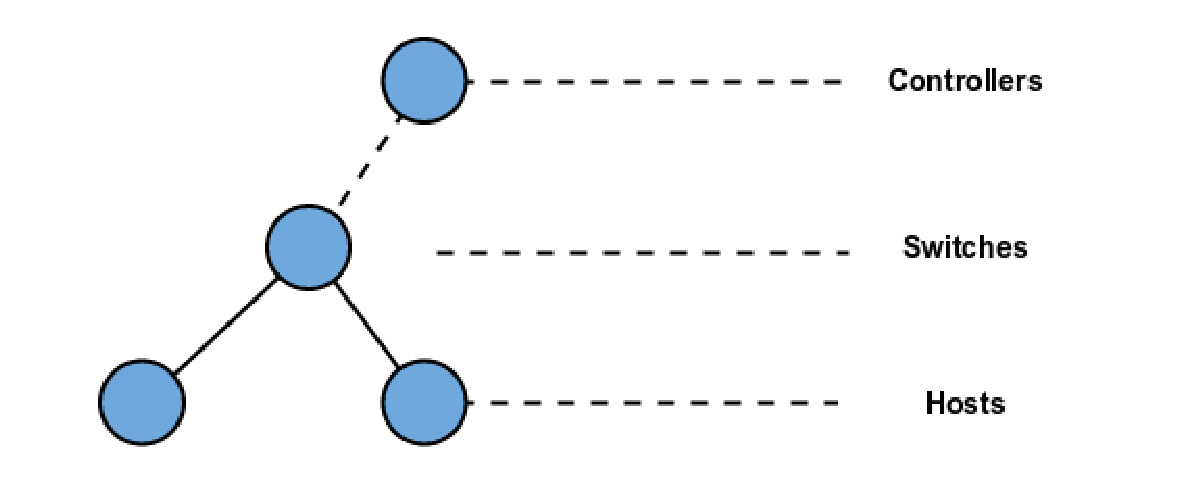
\includegraphics[scale=0.6]{./figuras/mininet1}
\caption{Topología creada con el comando \textit{sudo mn}.}
\label{mininet1}
\end{figure}

\subsection{Historia y desarrollo}
\emph{Mininet} está basado en los procesos de virtualización mediante el espacio de nombres en Línux\cite{mininetHistory}. Gracias al espacio de nombres, Bob Lantz y Brandon Heller desarrollaron el primer prototipo de mininet, la versión 1.0. A partir de esta primera versión, gracias al esfuerzo de James Page (y el apoyo de \textit{C}anonical y \textit{Big Switch}), se creó el sistema de paquetes que permite la instalación de mininet en Ubuntu de forma sencilla. Este fue un gran paso que permitió acercar mininet a todos los usuarios.

Al ser un proyecto de tipo \textit{OpenSource}, la colaboración estuvo garantizada desde el principio, consiguiendo mayor difusión, mayor aceptación y un mejor reporte de fallos y soporte. Con el esfuerzo de la comunidad y apoyos de varias organizaciones (Stanford u ON.lab por ejemplo), el desarrollo de mininet fue rápido, y se fueron sucediendo las diferentes versiones. La versión actual es la versión 2.2.1.

\emph{Mininet} es desarrollado por contribuidores y miembros del núcleo. Los desarrolladores principales son seis, mientras que entre los contribuidores, podemos encontrar más de 27. Todo esto sin contar a todos aquellos usuarios de la comunidad que reportan fallos y/o intentan arreglar dichos fallos. proponiendo cambios a los miembros desarrolladores. 

\emph{Mininet} es otra muestra del crecimiento fugaz de los proyectos de tipo abierto, gracias al apoyo de la comunidad.

\subsection{Comparativa}
\emph{Mininet} no es la única herramienta para emulación de redes, existen alternativas. En esta subsección vamos a comparar mininet con \textit{EstiNet}\cite{estinet}, apoyándonos en los resultados presentados \cite{wang2014comparison}. \textit{EstiNet} es una herramienta que permite tanto emular como simular redes.

Un simulador es software que predice el comportamiento de una red de acuerdo a unos parámetros y modelos definidos. Los parámetros estarán, normalmente, definidos por el usuario, para adaptar el comportamiento simulado al comportamiento real que se desee. La simulación podrá simular fallos o cambios de red, en tiempo real o planificados, entre otras muchas posibilidades. Existe un gran número de simuladores que permiten predecir el comportamiento de casi cualquier protocolo de red en una situación definida. La predicción se lleva a cabo mediante el uso de modelos matemáticos sobre: fuentes de datos, canales, elementos y protocolos. 

En contraposición a la simulación se encuentra la emulación. En emulación se pretende parecer una red real ejecutando, el mismo código que ejecutaría el dispositivo emulado, permitiendo así obtener datos y eventos "idénticos" a los que sucederían en una red real. Las redes son imperfectas, aparecen eventos no previstos continuamente, afectando al resultado de los datos obtenidos. Emulando se pretende que esta parte aleatoria, que no puede ser controlada (solo estimada) en simulación, esté prevista y sea recogida en tiempo real. 

Como resumen podemos destacar que simulación es una buena solución (básica a día de hoy para probar nuevas tecnologías), capaz de dar resultados fiables en entornos controlados. Además simulación es una solución muy escalable al poder ser todo controlado en un mismo equipo. Emulación introduce la probabilidad de que no todo vaya según lo previsto, al ser una ejecución en tiempo real, que recoge todos los eventos posibles en una red. Existen otras muchas características que podrían ser comparadas entre emulación y simulación, pero para nosotros, la fidelidad a la realidad (y la posibilidad de reproducir fallos o errores), es la más importante a la hora de comprobar el funcionamiento de la aplicación que queremos evaluar.

Para emular redes existen diferentes soluciones. En el artículo \cite{wang2014comparison} se comparan \textit{EstiNet} y mininet.

\subsubsection{Emuladores de red.} Existen dos emuladores principales de red, \emph{Mininet} y \textit{EstiNet}. Mientras el primero de ellos es de tipo abierto y colaborativo, el segundo es una solución privada y cerrada. Esta será una razón importante para que se haya elegido \emph{Mininet} como herramienta de emulación. 

Los dos emuladores tienen una filosofía muy diferente. En EtsiNet cada vez que se genera un paquete en un \textit{host}, este paquete es procesado por un \textit{socket} Línux real del tipo \textit{socket/TCP/IP}. Tras ser procesado por el \textit{socket}, se crea un túnel que conecta con la emulación o simulación, y que procesa paquetes que se transportan sobre protocolos por debajo de \ac{IP}. Estas capas de red emuladas, simulan todos los efectos que podría sufrir el paquete en una red real antes de enviarlo al destino. Los \textit{sockets} Línux están integrados en el \textit{kernel} del \ac{SO}. Este modo de trabajo permite que cada \textit{switch} emulado, pueda establecer una conexión \ac{TCP} real con los controladores \emph{OpenFlow} reales, imitando de forma fiel el comportamiento del protocolo \emph{OpenFlow}.

\emph{Mininet} por su parte recurre a la virtualización de elementos para conseguir la emulación de red. Para poder distinguir interfaces de tablas de \textit{routing} y demás elementos, hace uso del espacio de nombres definido en Línux desde la versión 2.2.26 del \textit{kernel}. Para la virtualización de \textit{switches} \emph{OpenFlow}, \emph{Mininet} usa \textit{Open vSwitch}, integrado totalmente en el \textit{kernel} de Línux. Las conexiones \textit{ethernet} también están virtualizadas gracias al \textit{kernel}. Cada paquete inyectado en la red es procesado por la pila de protocolos de Línux, otorgando realismo al proceso. El único problema que puede encontrar \emph{Mininet} es el de escalabilidad, ya que todos los elementos virtuales comparten la misma CPU, siendo en algunos casos muy complicado para el planificador de Línux cumplir todos los requisitos. En las últimas versiones de \emph{Mininet} se incluye la posibilidad de conectar la red por alguna interfaz con el exterior, con lo que parte de la red podría ser emulada en otro equipo, solucionando este problema.

Según los resultados obtenidos en \cite{wang2014comparison}, se puede decir que el emulador EtsiNetm obtiene resultados muy precisos hasta que el número de elementos se vuelve demasiado elevado (961), a partir de este número de elementos, los resultados se desvían de los resultados esperados. El simulador EtsiNet obtiene unos buenos resultados en lo referente a escalabilidad y precisión, sin embargo la simulación ocupa un mayor tiempo que la emulación, además los recursos usados son mayores. Por último \emph{Mininet} muestra un buen comportamiento, sin embargo (según el estudio), devuelve resultados inconsistentes bajo algunas condiciones de red (carga alta o casos especiales).

Los resultados obtenidos en el estudio \cite{wang2014comparison} dan EtsiNet un paso por delante de \emph{Mininet}. Sin embargo, la comunidad que apoya este último, la ayuda que puede ser encontrada y ser de tipo abierto, hacen de \emph{Mininet} la mejor opción para el desarrollo de este proyecto.

Otra medida interesante para comparar las dos herramientas, es la que se obtiene al comparar los resultados obtenidos en Google a 18 de Junio de 2014. La búsqueda de los términos \textit{EstiNet} y \emph{Mininet} deja una comparativa sobre la relevancia de cada uno. El primero obtiene 16200 resultados en 0.3 segundos según Google. \emph{Mininet} por su parte consigue 467.000 resultados en 0.4 segundos. Esta diferencia de casi 30 veces más resultados de \emph{Mininet} frente a \textit{EstiNet}, es una muestra de la aceptación de uno y otro. 

Por último se quiere destacar que el blog desarrollado en paralelo a este trabajo, \url{http://www.aprendiendoodl.wordpress.com}, se sitúa en el puesto 15 de los resultados arrojados por Google para el término de búsqueda \emph{Mininet}, siendo un dato interesante para evaluar el alcance que puede llegar a tener este proyecto.

\subsection{Diseño de redes}\label{pythonapi}
Para el diseño de redes, \emph{Mininet} cuenta con una \ac{API}\cite{mininetAPI}, escrita en Python, que permite diseñar y ejecutar casi cualquier tipo de red. Existen numerosos ejemplos por la red de uso, además de los que se encontrarán en este trabajo por lo que no vamos a tratar en profundidad como definir redes en \emph{Mininet}. 

\begin{figure}
\centering
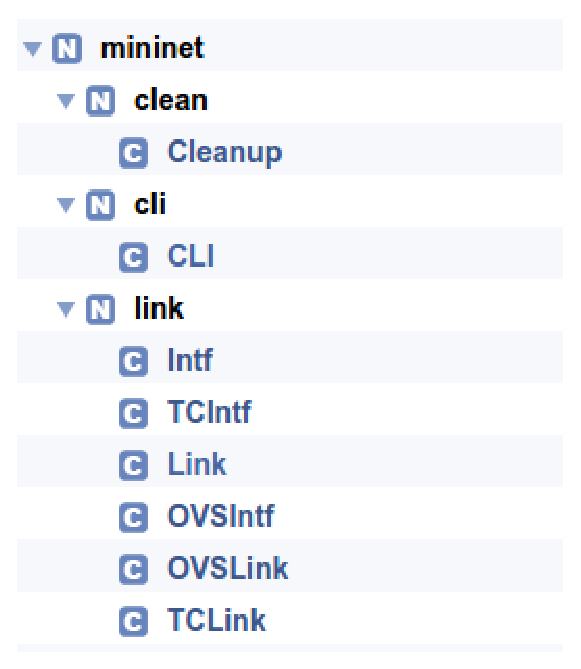
\includegraphics[scale=0.8]{./figuras/mininetAPI}
\caption[Ejemplo clases Python]{Algunas de las clases de la \emph{Mininet} Python \ac{API}. Imagen tomada de \cite{mininetAPI}}\label{pythonAPI}
\end{figure}

\section{\emph{OpenDayLight}}
En la sección \ref{opendaylight} se ha descrito \emph{OpenDayLight} de forma teórica, es el momento de comenzar a trabajar con la implementación software del controlador. En esta sección van a ser tratadas las versiones existentes del controlador, justificaremos la elegida, y finalmente haremos hincapié en las posibilidades de desarrollo de aplicaciones para éste.

\subsection{Distribucciones y versiones}
Desde la primera versión hasta hoy, el proyecto \emph{OpenDayLight} ha ido lanzando nuevas versiones de su controlador. En tan solo dos años, el proyecto ha lanzado más de 5 versiones estables finales, lo que es una clara muestra del interés generado en torno al proyecto. Las versiones sucesivas han ido añadiendo características al núcleo de \ac{ODL}, mejoras de funcionalidad y otras innovaciones. A continuación se han resumido brevemente las versiones disponibles para \emph{OpenDayLight}.

\subsubsection{Versiones Hydrogen.} 

Fueron las primeras versiones del controlador \emph{OpenDayLight}, se lanzaron tres versiones diferentes a la vez: básica, virtualización y proveedor de servicios. Cada una de estas versiones estaba destinado a proyectos concretos como su propio nombre indica. Todas estas versiones están basadas en los siguientes conceptos:

\begin{itemize}
\item[•] \textbf{Maven.} Maven permite a \emph{OpenDayLight} una fácil automatización a la hora de construir aplicaciones. A través del fichero pom.xml de Maven, \ac{ODL} sabe que módulos debe cargar e iniciar. Se describirá exhaustivamente en la sección \ref{sub:desarrollo}.

\item[•] \textbf{OSGi.} OSGi es un framework que permite la carga dinámica de bundles y paquetes (archivos JAR). Además permite enlazar \textit{bundles} para el intercambio de información. Se describirá ampliamente en la sección \ref{sub:desarrollo}.

\item[•] \textbf{JAVA interfaces.} Son usadas para el intercambio de información y para la especificación de eventos de escucha. A través de JAVA se definen funciones \textit{call-back}, que permitirán que posteriormente las aplicaciones sean llamadas cuando sucedan eventos, o que las propias aplicaciones generen eventos.

\item[•] \textbf{\ac{REST} \ac{API}s.} \ac{API}s \textit{Northbound} que permitirán a las aplicaciones la comunicación y obtención de información con el controlador (vía web). 
\end{itemize}

Estas primeras versiones incluían ya un buen número de proyectos (ampliados en las siguientes), para facilitar y posibilitar el uso de capacidades de red, como por ejemplo control de la capa física u obtención de información acerca del estado de red. Además se incluyó desde el principio compatibilidad con las versiones 1.0 y 1.3 de \emph{OpenFlow}. Entre las características iniciales también se incluyó una interfaz web que permitía el control de red de forma gráfica, como se aprecia en la imagen \ref{dlux}.

\begin{figure}[tb]
\centering
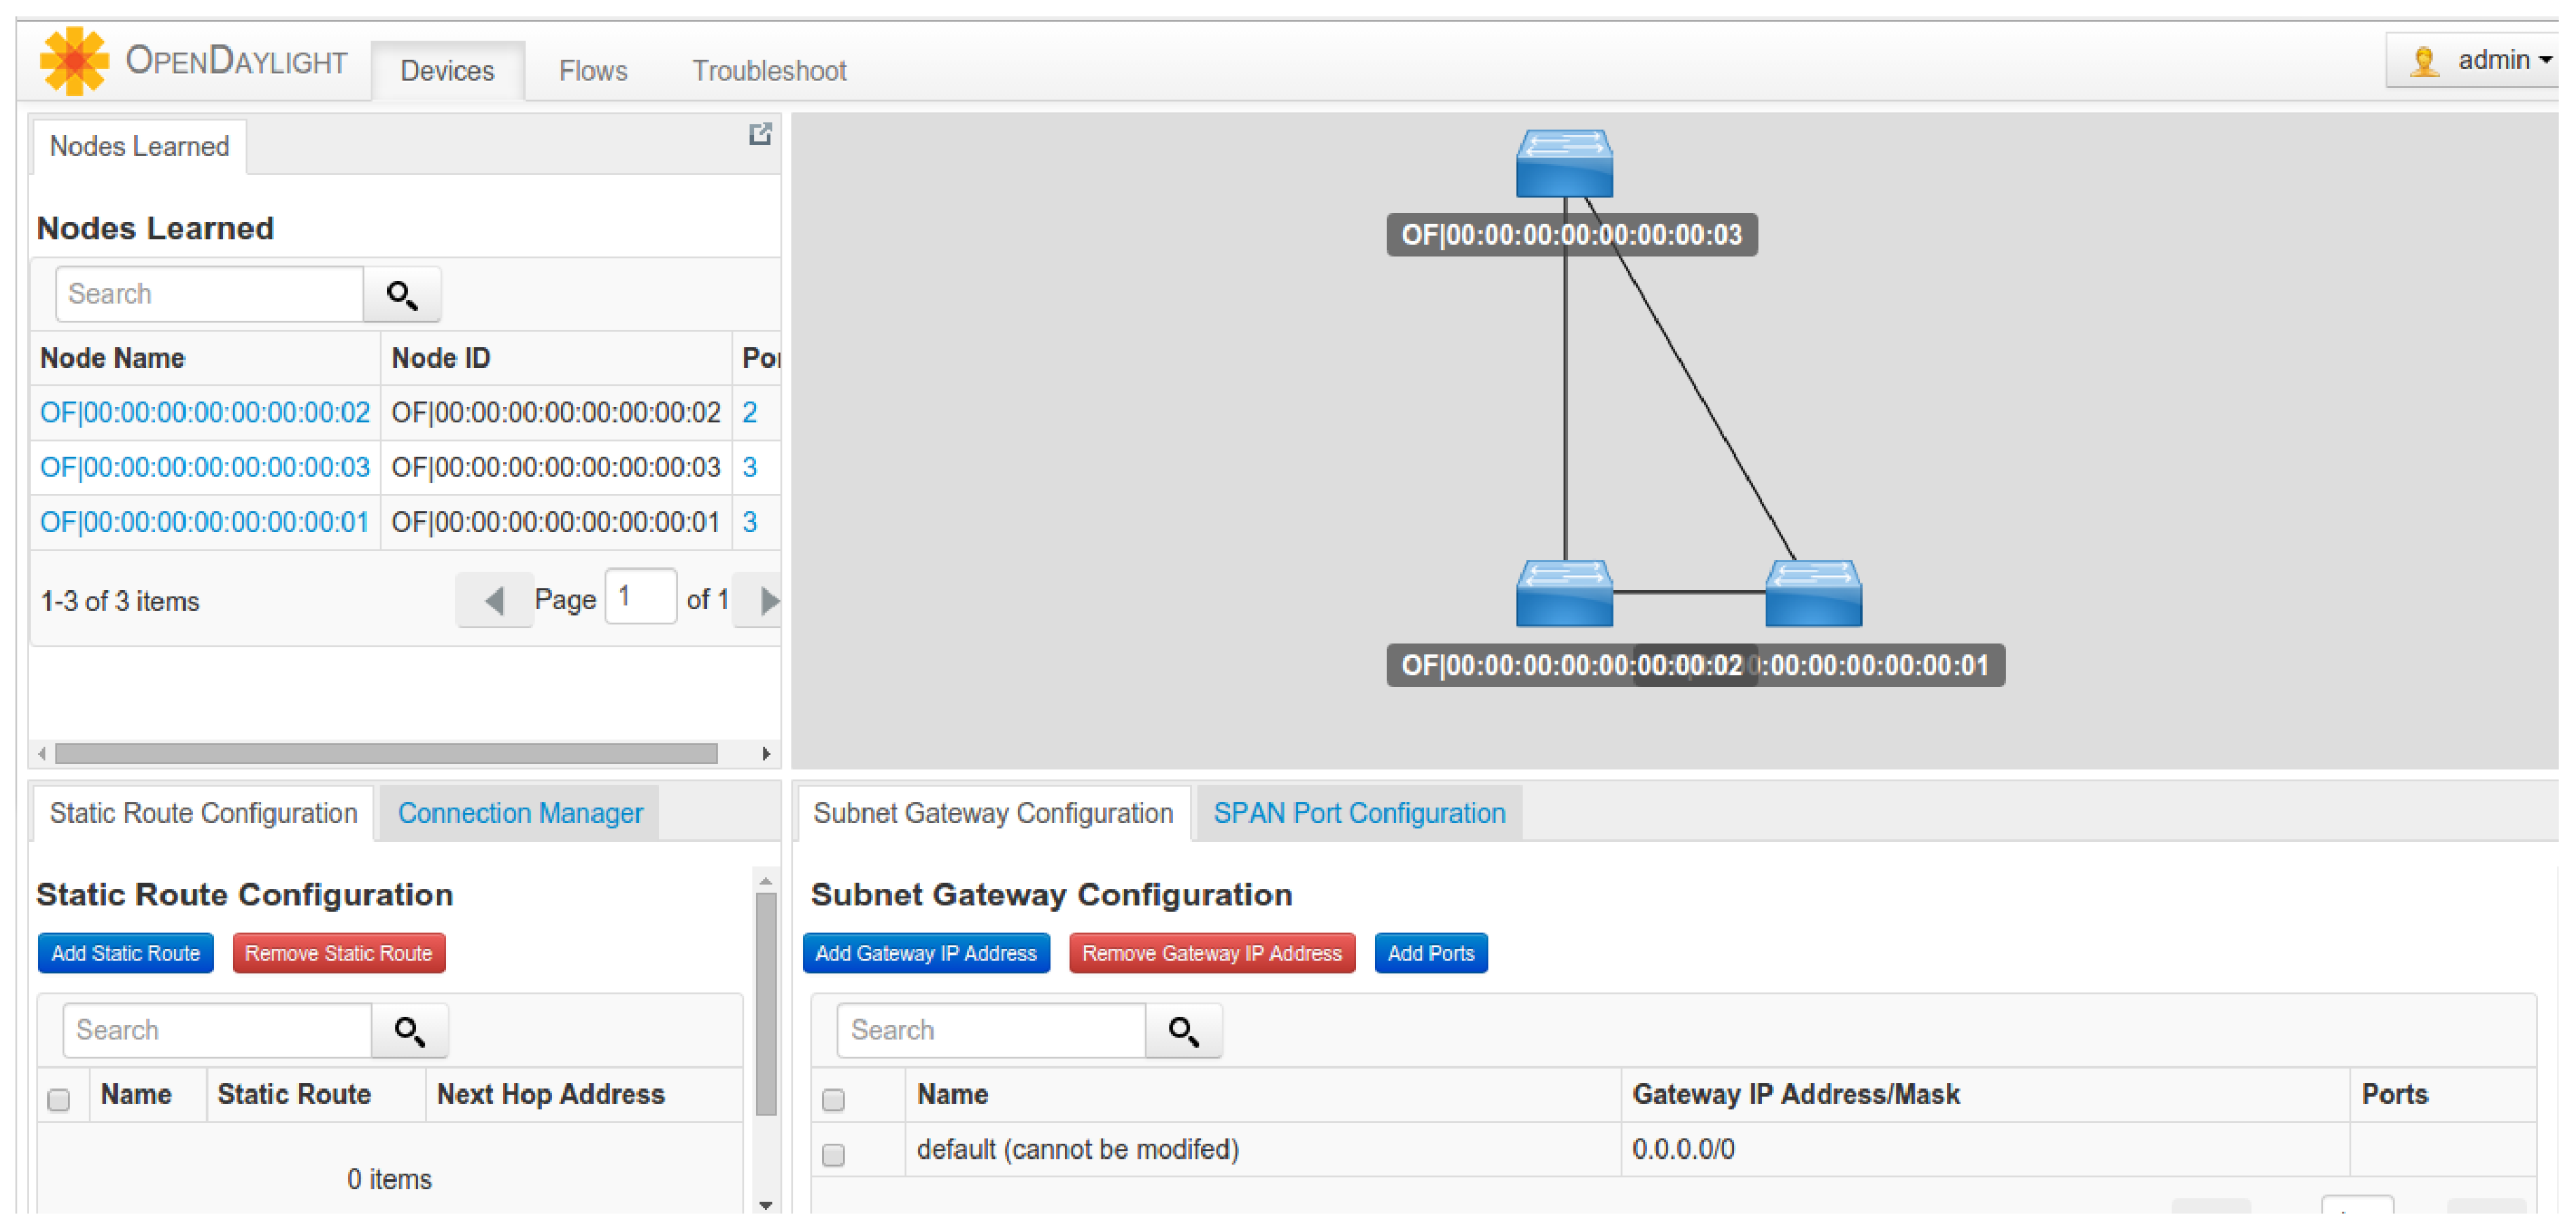
\includegraphics[scale=0.333]{./figuras/dlux1}
\caption{Interfaz web versión base \ac{ODL}}\label{dlux}
\end{figure}

\emph{OpenDayLight} siguió trabajando en el núcleo del controlador, lanzando sucesivas versiones de éste. Una de estas versiones fue elegida para realizar el proyecto, la versión base 0.2.2\footnote{https://nexus.opendaylight.org/content/repositories/opendaylight.snapshot/org/opendaylight/integration/distributions-base/0.2.2-SNAPSHOT/}. Se eligió esta versión por dos motivos: primero, al momento de comenzar este trabajo se acababa de lanzar la versión Helium (que describiremos a continuación), que suponía un cambio respecto a las anteriores, con lo que la información sobre esta versión era escasa y un tanto difusa. La segunda razón es que la versión elegida ofreció un buen funcionamiento desde el principio con los módulos propuestos en el trabajo en ese momento, lo cual marcó nuestra elección\footnote{Existe una versión posterior a la 0.2.2, 0.3.0, que fue descartada por problemas con los módulos para instalar flujos.}.

\subsubsection{Helium.} Heliumfues la apuesta de \ac{ODL} para hacer su controlador más accesible y cómodo al usuario. El núcleo del controlador siguió siendo el mismo que en Hydrogen (con las mejoras propias de las sucesivas versiones), pero en lo referente a la interfaz se produjo una revolución. Helium apostó por integrar karaf\cite{karaf}. Karaf proporciona un contenedor de aplicaciones y componentes que se pueden implementar al mismo tiempo y de forma dinámica. Basado en OSGi, proporciona facilidad de uso cuando se usan un gran número de componentes y módulos.

\begin{figure}[tb]
\centering
%\hspace*{-1.5cm}
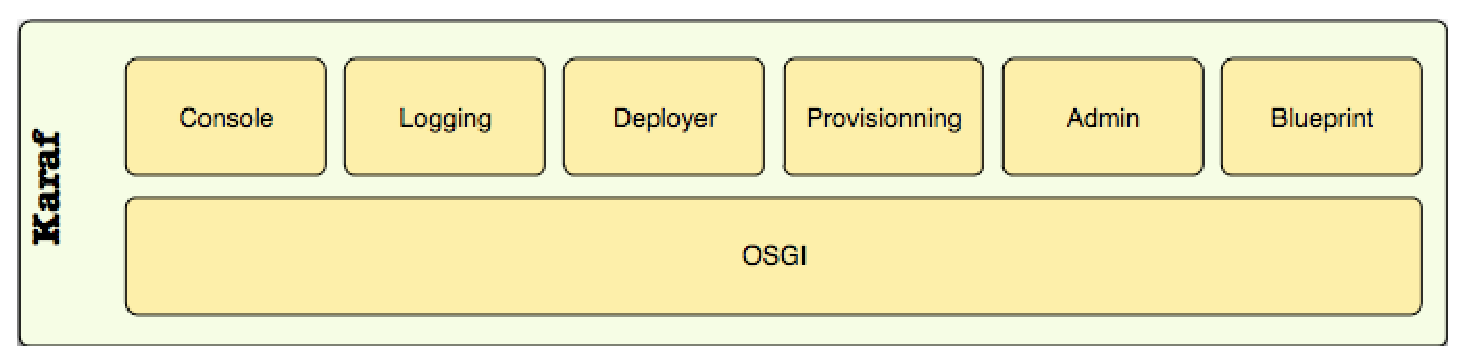
\includegraphics[scale=0.65]{./figuras/karaf}
\caption{Esquema básico de karaf.}\label{karaf}
\end{figure}

Además de este cambio en la forma de mostrarse al usuario, con Helium se lanzaron una serie de mejoras, como la inclusión de la interfaz web DLUX (una versión muy mejorada de la anterior interfaz), que permite un gran número de opciones de control y administración de red, como se aprecia en la figura \ref{dlux2}. Muchos de los componentes del núcleo \emph{OpenDayLight}, y muchos aplicaciones siguen en continuo desarrollado y pueden ser instaladas y actualizadas de forma sencilla gracias al uso de karaf. 

\begin{figure}[tb]
\centering
%\hspace*{-1.5cm}
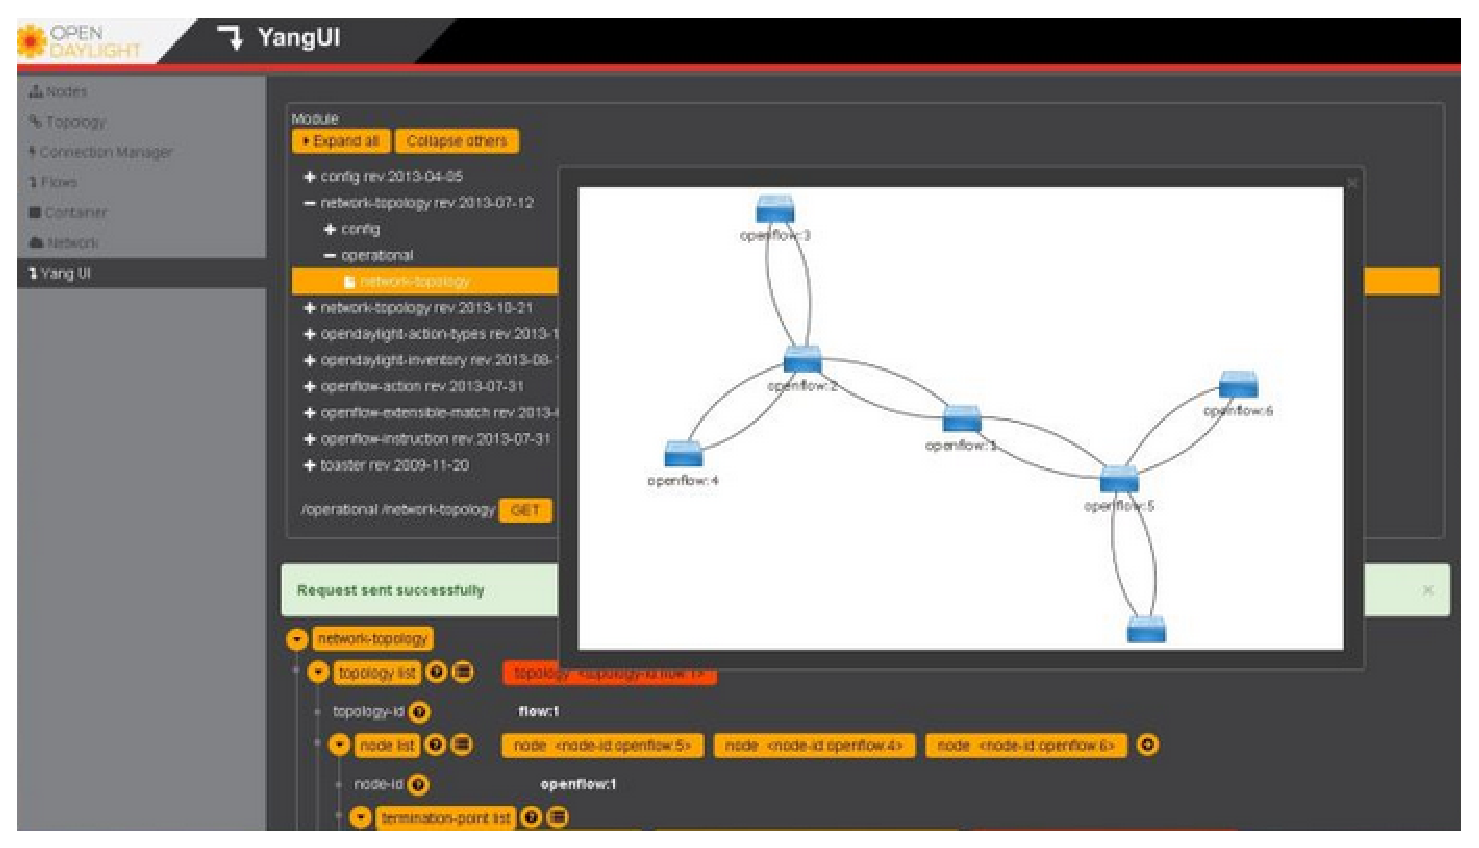
\includegraphics[scale=0.65]{./figuras/dlux2}
\caption{Interfaz web \ac{ODL} con la versión Helium.}\label{dlux2}
\end{figure}

Helium ha tenido un desarrollo muy rápido y se han ido sucediendo las versiones de forma fugaz (en menos de 6 meses han sido lanzadas 4 versiones del controlador), mejorando en todas ellas diferentes funcionalidades.

\subsubsection{Lithium}

El día 29 de Junio de 2015 se lanzó una nueva versión del controlador \emph{OpenDayLight}. Debido a lo ajustado del calendario no se ha realizado un estudio sobre los cambios que introduce esta nueva versión, sin embargo se cree necesaria la inclusión de esta nueva versión en el documento.

Como ya se ha comentado, se ha elegido para trabajar la versión base 0.2.2 en este proyecto. Esto no debería suponer un impedimento (en teoría) para poder usar la aplicación desarrollada en este trabajo con cualquier otra versión \emph{OpenDayLight}. Sin embargo pueden existir problemas de compatibilidad con las actualizaciones de algunos de los módulos usados. Una de las vías de trabajo futuras podría ser intentar desarrollar y/o adaptar los módulos desarrollados para las primeras en las nuevas versiones \ac{ODL}, que serán más eficientes y tendrán un mayor número de funcionalidades.

\subsection{Desarrollo}\label{sub:desarrollo}
Existen varias opciones para llevar a cabo el desarrollo de una aplicación (o cualquier otra funcionalidad) en \emph{OpenDayLight}. En las primeras versiones del controlador se usó una abstracción conocida como \ac{AD}-\ac{SAL}. \ac{AD}-\ac{SAL}, que permitía el desarrollo de aplicaciones para el controlador, sin preocuparse por el protocolo que controlará la red \ac{SDN}. De este modo se posibilitó el desarrollo aplicaciones independientes del tipo de elemento de red, que posteriormente recibía las instrucciones generadas por las aplicaciones. En las primeras versiones del controlador esta capa de abstracción permitía obtener información acerca de los vecinos de un elemento de red, o las propiedades de una interfaz de cualquier elemento, entre otras muchas características.

Posteriormente se desarrolló \ac{MD}-\ac{SAL}, una mejora de la anterior capa de abstracción. La abstracción por modelos se presentó como una oportunidad para unificar todas las \ac{API}s (\textit{SouthBound} y \textit{Northbound}), y las estructuras de datos usados en los componentes de un controlador \ac{SDN}. Para describir las estructuras de datos se propuso un lenguaje de modelado, YANG \cite{bjorklund2009yang}. Con este lenguaje de modelado se permitió modelar todas las estructuras de datos y funcionalidades proporcionadas por los componentes del controlador, definir relaciones entre elementos y modelar todos los componentes de un sistema. YANG es un lenguaje de naturaleza \ac{XML}. Utilizando un esquema de lenguaje simplificado como éste, se simplificó el desarrollo de componentes y aplicaciones para el controlador. Un desarrollador podía describir un módulo definiendo tan solo el esquema, y crear, a partir de dicho esquema, la funcionalidad mediante alguno de las \ac{API}s permitidas.

En la tabla \ref{comparativaSAL} se resaltan las diferencias entre las posibilidades.

\begin{table}[tb]

\centering
\hspace*{-1.3cm}
\resizebox{18cm}{!}{
\begin{tabular}{|c|c|}
\hline
{\bf \ac{AD}-\ac{SAL}}                                                                                                                                                                                                                 & {\bf \ac{MD}-\ac{SAL}}                                                                                                                                                                                \\ \hline
\begin{tabular}[c]{@{}c@{}}Las \ac{API}s de abstracción solicitan\\ rutas entre consumidores y proveedores.\\ Las adaptaciones se definen de forma estática\\ al compilar.\end{tabular}                                           & \begin{tabular}[c]{@{}c@{}}Las \ac{API}s de abstracción solicitan\\ las rutas mediante la definición de modelos,\\ y las adaptaciones son realizadas en tiempo\\ de ejecución.\end{tabular}      \\ \hline
\begin{tabular}[c]{@{}c@{}}Es necesaria una \ac{REST} \ac{API} dedicada\\ para cada \ac{NB} y \ac{SB} plugin\end{tabular}                                                                                                                        & \begin{tabular}[c]{@{}c@{}}Proporciona una \ac{REST} \ac{API} común para \\ acceder a datos y funciones definidos en modelos\end{tabular}                                                             \\ \hline
Provee servicios de adaptación para plugins                                                                                                                                                                                  & \begin{tabular}[c]{@{}c@{}}No provee de servicios de adaptación para\\ plugins\end{tabular}                                                                                                 \\ \hline
\begin{tabular}[c]{@{}c@{}}Las peticiones de routing están basadas en el \\ tipo de plugin. Cuando un plugin \ac{NB} solicita \\ una operación en un nodo dado,  el plugin\\ \ac{SB} se encarga de encaminar a dicho nodo\end{tabular} & \begin{tabular}[c]{@{}c@{}}Las solicitudes en \ac{MD}-\ac{SAL} se realiza de forma\\ dinámica ya que los datos del nodo se exportan\\ de forma automática al \ac{SAL}\end{tabular}                         \\ \hline
\ac{AD}-\ac{SAL} no comparte datos                                                                                                                                                                                                     & \begin{tabular}[c]{@{}c@{}}Los datos de modelos definidos por plugins\\ pueden ser intercambiados entre consumidores \\ y proveedores a través del almacenamiento en \\ \ac{MD}-\ac{SAL}\end{tabular} \\ \hline
\begin{tabular}[c]{@{}c@{}}Los servicios en \ac{AD}-\ac{SAL} suelen proveer \\ funciones síncronas y asíncronas\end{tabular}                                                                                                           & \begin{tabular}[c]{@{}c@{}}\ac{MD}-\ac{SAL} se enfoca hacia \ac{API}s asíncronas, \\ permitiendo sin embargo bloquear procesos para\\ posibilitar comunicaciones síncronas\end{tabular}                    \\ \hline
\end{tabular}
}
\caption[Comparativa \acs{AD}-\acs{SAL} y \acs{MD}-\acs{SAL}]{Diferencias entre las capas de abstracción \ac{AD}-\ac{SAL} y \ac{MD}-\ac{SAL}. Tabla tomada de \cite{comparativeSAL}}
\label{comparativaSAL}

\end{table}

Para desarrollar una aplicación para el controlador usaremos \ac{MD}-\ac{SAL}, por todas las ventajas que genera. Para el desarrollo emplearemos algunas de las \ac{API}s definidas en \cite{developerGuide}.

\subsubsection{\ac{DOM} \ac{API}\cite{dom}.} \ac{DOM} es una interfaz de programación para documentos \ac{HTML} y \ac{XML}. Facilita una representación estructurada del documento y define de qué manera los programas pueden acceder para modificar estructura, estilo y contenido. \ac{DOM} es una representación del documento como un grupo de nodos y objetos estructurados que tienen propiedades y métodos. Esencialmente, conecta las páginas web a \textit{scripts} o lenguajes de programación.

Una página web es un documento. Éste documento puede mostrarse en la ventana de un navegador o también como código fuente \ac{HTML}. En ambos casos, es el mismo documento. \ac{DOM} proporciona otras formas de permite otra manera, guardar y manipular este mismo documento. \ac{DOM} es una representación completamente orientada al objeto de la página web para ser modificado por \textit{scripts} o código progamado.

Como \ac{API}, \ac{DOM} se desarrolló posteriormente a las primeras versiones de \emph{OpenDayLight}, como respuesta a las necesidades planteadas por la comunidad. \emph{OpenDayLight} evoluciona en función de las necesidades de los usuarios.

\subsubsection{\ac{REST} \ac{API}.} Cuando hablamos de \ac{REST} nos referimos a cualquier interfaz entre sistemas que utilice directamente \ac{HTTP} para la comunicación en cualquier formato (\ac{XML}, \ac{JSON}, etc). En \emph{OpenDayLight} \ac{REST} se base en RestConf, \cite{restODL} y \cite{restODL2}, que es un protocolo implementado en el \ac{SAL} de \emph{OpenDayLight}. Los datos están definidos en YANG. El almacenamiento está definido por \ac{NETCONF}, usando \textit{Restconf} (protocolo sobre \ac{HTTP}). Lo que hace \textit{Restconf}, es describir como mapear una especificación YANG para una interfaz \ac{REST}. 

La \ac{REST} \ac{API} proporciona una interfaz simplificada adicional para el uso de \ac{NETCONF}, a través del protocolo \textit{Restconf}. \textit{Restconf} permite acceder a los \textit{datastore} definidos por YANG en el controlador. Existen dos almacenes de datos, configuración y operacional. 

En \emph{OpenDayLight} la escucha de peticiones se hace a través del puerto 8080 (\ac{HTTP}). Cuenta con las siguientes operaciones disponibles:
OPTIONS, GET, PUT, POST, DELETE. Estas peticiones podrán ir en formato \ac{JSON} o \ac{XML}, siempre de acuerdo con el modelo YANG definido.
 
Uno de los problemas a la hora de usar \ac{REST} \ac{API} es su carácter pro activo, ya que no existirán funciones de aviso capaces de informar sobre eventos de red en tiempo real (no existen métodos de escucha soportados, al menos encontrados durante este trabajo), con lo cual no se podrá reaccionar de forma automática ante cambios en la red.

\subsubsection{JAVA \ac{API}.} JAVA es un lenguaje de programación orientado a objetos muy extendido. Gracias a los servicios de abstracción implementados en \emph{OpenDayLight}, se permite que cada proveedor desarrolle su propia \ac{API} para la programación. Las \ac{API}s de este tipo también incluyen funcionalidades para acceder a los datos mediantes \ac{REST}, sin embargo (por conocimiento del lenguaje JAVA) se ha optado por realizar un desarrollo totalmente en JAVA sin hacer uso del resto de \ac{API}s. Haremos uso del JAVAdoc proporcionado por Cisco \cite{ciscojavadoc} (está definido para la adaptación de Cisco del controlador \emph{OpenDayLight}, DevNet), que recoge todas las clases disponibles desarrolladas para el controlador. \emph{OpenDayLight}, y las que además ha definido Cisco para su adaptación del controlador. 

Se ha elegido para el desarrollo el uso de la JAVA \ac{API} proporcionada por Cisco, por conocimiento del lenguaje de programación y por la posibilidad programar flujos de manera tipo reactiva, algo que es básico en recuperación de errores para \ac{QoE}, uno de los objetivos de este trabajo.

\section{Java}

JAVA es un lenguaje de programación orientado a objetos, que puede ser ejecutado en cualquier \ac{SO} gracias a la máquina virtual de JAVA. Es esta una de las principales razones por las que \emph{OpenDayLight} está desarrollado sobre este lenguaje, la compatibilidad. Siendo JAVA uno de los lenguajes de programación que se han estudiado a lo largo de la preparación universitaria del autor, parece lógica su elección como lenguaje para programar aplicaciones \ac{ODL}. 

También se tiene en cuenta que las \ac{API}s de JAVA proporcionan las funcionalidades necesarias para alcanzar los objetivos requeridos en el proyecto. 

Una vez escrito el código será necesario compilarlo para su posterior ejecución. Para esta tarea \emph{OpenDayLight} especifica como compilador Maven.

\subsection{Maven}
Maven \cite{maven} se inició como una herramienta para simplificar la compilación de proyectos JAVA. Se pretendió crear un estándar que: definiera de forma clara en que consistía el proyecto, mantuviera organizada toda la información relacionada con éste y simplificara el modo en que el proyecto depende del resto de librerias o módulos (a través de los archivos \ac{JAR}). El resultado es una herramienta que facilita el trabajo diario de los desarrolladores, ahorrando tiempo en la definición y compilación de proyectos, y simplificando las relaciones entre estos.

\begin{figure}[tb]
\centering

\includegraphics[scale=0.8]{./figuras/maven}
\caption{Logo maven}\label{logoMaven}
\end{figure}

Una buena definición de lo que Maven ha conseguido se puede encontrar en \cite{maven}. Permitir al desarrollador comprender todo un proyecto completo (relaciones de clases por ejemplo), en el menor tiempo posible, mediante las características de Maven:

\begin{enumerate}
\item Facilitar el proceso de compilación.
\item Proporcionar un sistema de compilación uniforme para todos los proyectos.
\item Proporcionar información de calidad sobre el proyecto.
\item Proveer de unas líneas de buenas prácticas para el desarrollo.
\item Permitir nuevas características en los proyectos, de forma transparente.
\end{enumerate}

Mientras estemos desarrollando un módulo \ac{ODL} comprobaremos la utilidad de algunos de estos puntos, por ejemplo el último, ya que cada vez que hagamos un cambio y compilemos el código, automáticamente esta nueva característica se instalara en el controlador sin necesidad de ninguna acción extra por nuestra parte. También veremos que cualquier error en la programación del código será reflejado al intentar compilar, proporcionando una información concreta y precisa para intentar resolver el problema.

La programación para el compilador Maven hará uso del archivo \ac{POM}.\ac{XML}. Este archivo es la unidad fundamental de trabajo Maven ya que en él se describen todos los detalles del proyecto, como la configuración o los repositorios donde se han de buscar librerías para el proyecto. También se especifican los parámetros de compilación (como donde instalar el \ac{JAR} resultante) o donde se encuentran los archivos fuente. También incluye la posibilidad de definir archivos test que comprueben la validez del código implementado, ahorrando tiempo en el proceso de pruebas. También se especifica aquí información del proyecto, como la versión, descripción, autores, etc.

El archivo \ac{POM}.\ac{XML} es esencial para el desarrollo. Para facilitar su comprensión se incluye en el apéndice \ref{pom.xml} el resultante del desarrollo de este proyecto. No se incluye todo el codigo del proyecto debido a su extensión, pero podrá ser consultado en el repositorio del proyecto\footnote{\url{https://github.com/alfonsito92/serverVideoApp}}.

\subsection{Atom}
A la hora de desarrollar un proyecto de gran extensión se hace imprescindible el uso de un asistente para la programación o \ac{IDE}. Existen muchos asistentes disponibles que además permiten la integración completa de Maven (como es el caso de eclipse \cite{eclipse}, que además es uno de los más extendidos y completos). Sin embargo en la realización de este trabajo se ha optado por un \ac{IDE} más ligero (en cuanto a número de complementos y posibilidades) como es Atom \cite{atom}. Atom es un asistente de desarrollo ligado a github (repositorio en el que está alojado el proyecto), con lo que la integración con el servidor de repositorios es total. 

\begin{figure}[tb]
\centering

\includegraphics[scale=0.2]{./figuras/atom}
\caption{Logo de ATOM \ac{IDE}}\label{logoAtom}
\end{figure}

Otro de los aspectos por los que se ha elegido este \ac{IDE}, es que no es necesario configurarlo para la compatibilidad con Maven, sino que simplemente nos podremos dedicar a programar el código. Además su simplicidad a la hora de instalar y usar en el \ac{SO} elegido, permite que no sea necesario preocuparse por otro aspectos ajenos al desarrollo de este trabajo.

Por último al no integrar Maven ha sido necesario un mayor esfuerzo en cuanto al desarrollo se refiere, lo que a la larga ha permitido un mejor aprendizaje sobre el funcionamiento y características de la aplicación desarrollada.

Por supuesto se puede usar cualquier otro \ac{IDE} e incluso existen guías de configuración, \cite{configuringEclipse} para eclipse.

Haciendo uso de las herramientas y software descrito en este capítulo, se desarrollará todo el sistema que se describe en el capítulo \ref{design}.



\chapter{Implementación de la solución}\label{implementing}

En el capítulo anterior nos hemos centrado en definir los elementos lógicos que compondrán el sistema. En este capítulo nos ocuparemos de describir la implementación del entorno de emulación y de la solución (tanto programación del bundle \ac{ODL} como la topología y configuración de \emph{Mininet}). Todas las herramientas que usaremos a continuación han sido configurados como se recoge en el apéndice \ref{configUbuntu}, \ref{configMininet} y \ref{configODL}.
 

\section{Configuración del entorno de red SDN sobre \emph{Mininet}}

 La solución propuesta se implementrá en una red SDN con \textit{switches} \emph{OpenFlow} y controlador \emph{OpenDayLight}. Para que tanto el desarrollo como la evaluación sean ágiles y repetibles, se usa \emph{Mininet} para desplegar una red emulada con todos los elementos descritos.
 Las topologías de red que se evaluarán serán diseñadas con la \ac{API} de Python, tal como se describió en la sección \ref{pythonapi}. En los diseños nos deberemos ocupar de definir los elementos que formarán parte de la red (\textit{hosts} y \textit{switches}), así como indicar a qué controlador ha de administrar los \textit{switches} (cada \textit{switch} puede estar conectado a más de un controlador).
 
\section{Descripción de los elementos de la red \ac{SDN} implementada}

Dentro de los equipos que compondrán la solución propuesta encontramos tres diferentes: \textit{hosts}, \textit{switches} \emph{OpenFlow} y controlador. \textit{Hosts} y \textit{switches} \emph{OpenFlow} estarán emulados gracias a \emph{Mininet}, indicando la dirección \ac{IP} del controlador (en nuestro caso estará ubicado en el mismo equipo físico). 

\subsection{\textit{Hosts}}
Los \textit{hosts} son equipos finales emulados por \emph{Mininet}, que podrán ejecutar cualquier comando o aplicación que esté disponible en el sistema Línux sobre el que se están ejecutando. Estos \textit{hosts} podrán actuar como servidores web (\ac{HTTP}) o clientes de vídeo \textit{streaming}, como ocurre en las capturas \ref{server} y \ref{client}.

\begin{figure}[tb]
\centering
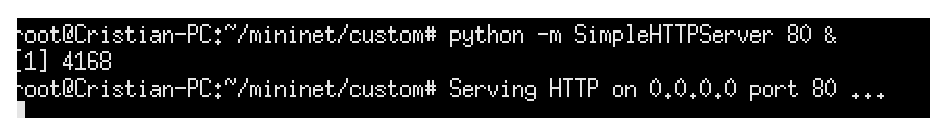
\includegraphics[scale=1]{./figuras/server}
\caption{Ejemplo servidor web en \textit{host} de \emph{Mininet}}\label{server}
\end{figure}

\begin{figure}[tb]
\centering
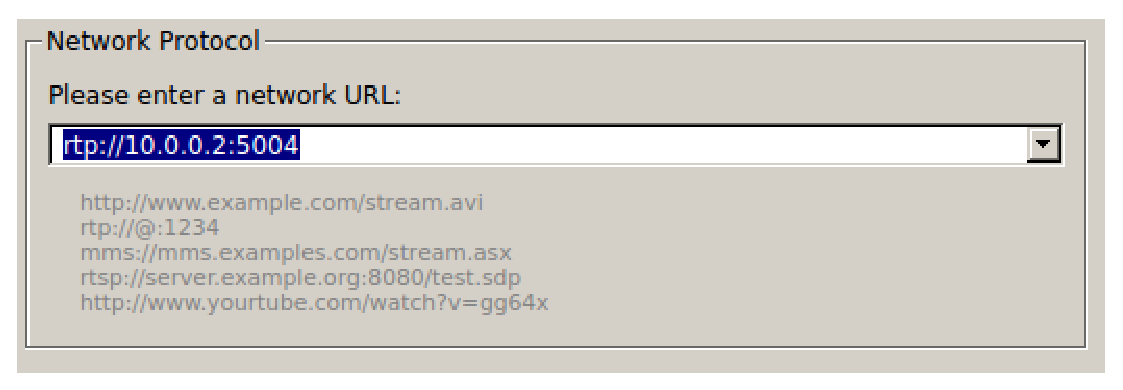
\includegraphics[scale=0.5]{./figuras/client}
\caption{Ejemplo cliente \ac{RTP} en \textit{host} de \emph{Mininet}}\label{client}
\end{figure}

El número de \textit{hosts} disponibles dependerá de los definidos en la topología que hayamos diseñado. En la mayoría de nuestras pruebas habrá 2 (cliente y servidor), sin embargo podrán coexistir tantos como sean necesarios (es posible que a partir de cierto número de equipos, los resultados obtenidos varíen con los teóricos como se estima en \cite{wang2014comparison}).

\subsection{Controlador}
El controlador \ac{ODL} será ejecutado en la misma máquina física donde estará corriendo \emph{Mininet}. Este controlador contará la aplicación diseñada ya instalada. También se eliminarán aquellos \textit{bundles} que manejen paquetes, para evitar incompatibilidades. En el apéndice \ref{configODL} se realiza una guía sobre la configuración del controlador \ac{ODL}.

La comunicación entre \textit{switches} \emph{OpenFlow} (siguiente subsección), se llevará a cabo haciendo uso del protocolo \emph{OpenFlow}, de acuerdo a la figura \ref{openflow1}. El controlador estará encargado de recibir los eventos que emitan los \textit{switches}, comunicarlo a los módulos y aplicaciones instalados, y comunicar hacia los equipos las instrucciones requeridas por estas aplicaciones y módulos.

\begin{figure}[tb]
\centering
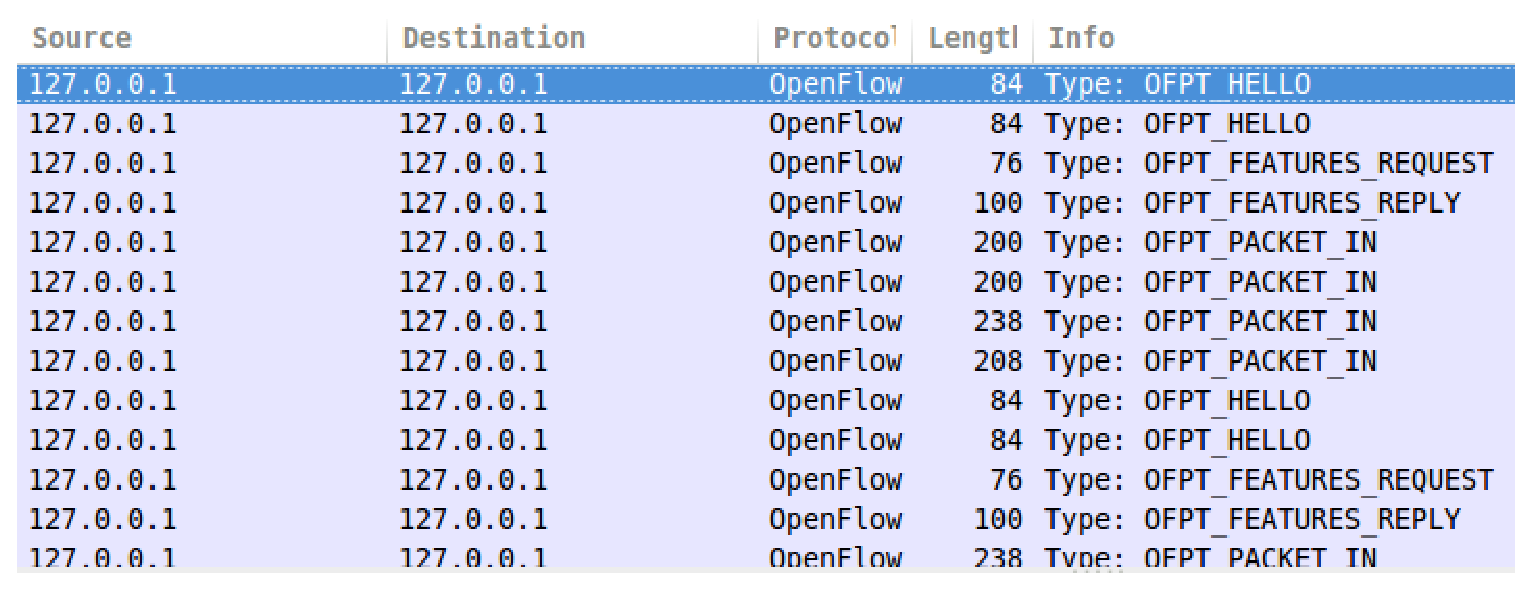
\includegraphics[scale=0.5]{./figuras/openflow1}
\caption{Ejemplo de comunicación \emph{OpenFlow} entre \textit{switches} \emph{Mininet} y controlador.}\label{openflow1}
\end{figure}

El controlador además será el encargado de recolectar (de forma automática) todas las estadísticas e información acerca del estado de la red, que posteriormente usaremos para la implementación del sistema.

\subsection{Elementos intermedios. \textit{Switches} \emph{OpenFlow}}
Los \textit{switches} \emph{OpenFlow} empleados por \emph{Mininet} estarán encargados de conformar la red de interconexión y además conectar con los \textit{hosts} finales. El encaminamiento en esta red vendrá dado por las indicaciones que el controlador comunique a los \textit{switches}. Como se ha estudiado en la sección \ref{openFlow}, estos \textit{switches} contarán con tablas y flujos para realizar el encaminamiento. 

Los \textit{switches} deberán comunicarse constantemente con el controlador, para actualizar estadísticas e información del estado de red, además en caso de eventos desconocidos (o instrucciones que requieran comunicación con el controlador) también deberán informar al controlador. 

Estos equipos estarán emulados gracias a virtualización. El software que usa \emph{Mininet} para virtualizar \textit{switches} y \textit{routers} es \textit{Open vSwitch} \cite{openvswitch}. \textit{Open vSwitch} es un conmutador virtual multicapa diseñado para automatizar la red mediante el uso de protocolos como \emph{OpenFlow}, pero sin dejar de lado otro tipo de protocolos de gestión. Otra de las características de su diseño es su filosofía de implementación real, ya que puede usarse en múltiples servidores físicos reales como los distribuidos por \textit{vmWare}. 

\begin{figure}[tb]
\centering
\includegraphics[scale=0.8]{./figuras/openvswitch}
\caption{Esquema de Open vSwitch.}\label{openvswitch}
\end{figure}

\subsection{Red de interconexión}
La red de interconexión hace referencia a los enlaces entre \textit{switches} \emph{OpenFlow}. Estos enlaces son provistos por la implementación en el \textit{kernel} de Línux. Los enlaces serán de tipo Ethernet (no se ha estudiado por ahora la posibilidad de uso de enlaces de fibra óptica u otros tipos). De estos enlaces se podrá configurar un gran número de parámetros, como latencia, probabilidad de pérdidas o ancho de banda, entre otras. 

El uso de este tipo de enlaces permitirá modificar la red en la que se evalúa el sistema, a fin de comprobar el comportamiento de la solución propuesta en diversos escenarios.

\subsection{Generación de escenarios en \emph{Mininet}}\label{sub:escenariosmininet}

Para la evaluación del sistema se usarán topologías que variarán en función de los resultados requeridos en cada caso. Una de las más usadas será la topología \ref{topologyBasic}, ya que cuenta con varios caminos para llegar al destino, con diferente número de saltos y permitirá comprobar la correcta evaluación de costes del capítulo \ref{cap:evaluation}.

\begin{figure}[tb]
\centering
\includegraphics[scale=0.7]{./figuras/topoBasic}
\caption{Topología básica para pruebas.}\label{topologyBasic}
\end{figure}

En esta topología (y en otras con diferente número de saltos), variaremos los parámetros de cada enlace y obtendremos los resultados requeridos. El código utilizado para esta topología básica se encuentra en el apéndice \ref{ap:pythonBasic}, con los siguientes parámetros:

\begin{center}
$BW = 10 Mbps $     \\  $latency = 10 ms$ \\ $loss(\%) = 0$
\end{center}

Siguiendo este esquema se construirán todas las topologías necesarias para evaluar la solución propuesta.

\section{OpenDayLight}
Para ejecutar el controlador tan solo lo descargaremos del enlace correspondiente\footnote{Para la versión elegida 0.2.2 el enlace es \url{https://nexus.opendaylight.org/content/repositories/opendaylight.snapshot/org/opendaylight/integration/distributions-base/0.2.2-SNAPSHOT/}}. Una vez descargado y descomprimido tan solo será necesario ejecutarlo y comprobar el correcto funcionamiento de todos los componentes. En caso de existir algún problema con la ejecución se aconseja consultar el apéndice \ref{configODL}. 

Si la ejecución es correcta tendremos en terminal una consolo OSGi (o karaf si es una versión superior\footnote{Para obtener los mismos resultados con karaf será necesario instalar módulos adicionales para el manejo de paquetes}), y podremos ejecutar una topología de \emph{Mininet} (como la topología básica del apéndice \ref{ap:pythonBasic}), indicando que el controlador está en la dirección 127.0.0.1 (mismo equipo). Si todo va bien y se realiza la conexión podremos realizar Ping entre los \textit{hosts} de la topología como en la imagen \ref{correctPing}.

\begin{figure}[tb]
\centering
\includegraphics[scale=0.5]{./figuras/prueba1}
\caption{Terminal mientras se está ejecutando el controlador \ac{ODL}.}\label{algo}
\end{figure}

\begin{figure}[tb]
\centering
\includegraphics[scale=0.5]{./figuras/prueba2}
\caption{Prueba de transmisión de ping con el controlador \ac{ODL}.}\label{correctPing}
\end{figure}

Además podremos comprobar que se han instalado flujos \emph{OpenFlow}, de igual manera que se realiza en la imagen \ref{correctFlows}.

\begin{figure}[tb]
\centering
\includegraphics[scale=0.5]{./figuras/prueba3}
\caption{Flujos instalados en S1 con el controlador \ac{ODL}.}\label{correctFlows}
\end{figure}

Si alguna de estas pruebas no resultase satisfactoria, en el apéndice \ref{problemas} pueden encontrarse diversas soluciones a problemas frecuentes. En caso no de resolver el problema, puede optar por visitar el blog del proyecto \url{http://www.aprendiendoodl.wordpress.com} y consultar las diferentes entradas, o dejar un comentario para que le intentemos ayudar.

Las aplicaciones preinstaladas que posibilitan la instalación de flujos (y que pueden causar conflictos con la desarrollada por no nosotros) son: \textit{simpleForwarding} y \textit{loadBalancer}. Podremos parar estos dos módulos (será necesario hacerlo cada vez que se inicie el controlador) o desinstalarlos por completo (permanente). Para parar los módulos tendremos que ejecutar (dentro de la consola OSGi):

\begin{center}
ss \textit{bundleName}
\end{center}

Lo cual nos devolverá el número de la aplicación. Con este número:

\begin{center}
stop \textit{bundleNumber}
\end{center}

Si queremos desinstalar los módulos podremos ir a la carpeta \textit{plugins} (del controlador descargado), y eliminar los \textit{bundles} necesarios. En esta carpeta será donde posteriormente instalaremos nuestra propia aplicación.

\section{Implementación en java}
Para desarrollar la aplicación que nos permita alcanzar los objetivos propuestos, usaremos el lenguaje JAVA. Como compilador se usará Maven. En esta sección vamos a describir como se ha implementado el código, como se compila con Maven y como instalar la aplicación en el controlador.

\subsection{Desarrollo Bundle Maven para ODL}
El desarrollo de un bundle para \ac{ODL} usando Maven se divide en dos partes: creación del archivo \ac{POM}.\ac{XML} y creación los archivos de código fuente JAVA. Dado que los ficheros de código fuente son muy extensos, no se ha querido sobrecargar esta memoria con ellos. Pueden ser consultados en el repositorio \url{https://github.com/alfonsito92/serverVideoApp}. Si se incluye el fichero \ac{POM} en el apéndice \ref{pom.xml}.

Para facilitar la descripción de todas las clases implementadas, en la figura \ref{clases} podemos apreciar las relaciones entre clases que se han definido\footnote{No se han incluido todas las clases ni métodos para facilitar la visión relación entre la clase principal y el resto.}\footnote{El resto de clases cuentan con los mismos métodos públicos (con diferente nombre) que la clase \textit{RTPRouting}.}.

\begin{figure}[tb]
\centering
%\hspace*{}
\includegraphics[scale=0.6]{./figuras/clases}
\caption{Relación \ac{UML} entre PacketHandler y RTPRouting.}\label{clases}
\end{figure}

Además en el repositorio se incluye el JAVAdoc generado con todos los métodos (públicos y privados) que se han usado. El archivo generado es el \textit{index.html} que se encuentra dentro de la carpeta \textit{doc}.

En este diagrama de clases se puede observar como se han añadido semáforos a la clase principal \textit{PacketHandler.java}. Estos semáforos evitarán que se accedan a datos al mismo tiempo, para evitar por ejemplo que intentemos instalar flujos en un \textit{switch} al mismo tiempo, o que se intente eliminar un flujo mientras se están leyendo.

Los archivos código fuente de JAVA para \emph{OpenDayLight} se dividen en dos grandes grupos, activador y manejador. En \cite{aprendiendoODL} existen varias guías y ejemplos sobre como comenzar con el desarrollo de componentes OSGi para \ac{ODL}.

El activador es el fichero donde se indica al controlador la clase manejadora y las relaciones con el resto de módulos \emph{OpenDayLight}, como por ejemplo que la aplicación implementará la \textit{interfaz de escucha de eventos de nuevo paquete}\footnote{La interfaz \textit{IListenDataPacket} permite implementar las acciones que realizará la aplicación cada vez que llegue un nuevo paquete al controlador.}, o que hará uso de interfaces para consultas de estadísticas o instalación de flujos. En el apéndice \ref{activator} se encuentra el fichero JAVA donde está definido el activador para este proyecto.

En nuestro caso será necesario implementar la funcionalidad para recibir eventos de nuevos paquetes, además deberemos hacer uso de:

\begin{itemize}
\item[•] \textbf{\textit{IDataPacketService}.} Esta interfaz permite la decodificación de paquetes (entrar dentro del paquete y analizarlo). Nos permitirá comprobar el tipo de paquetes.
\item[•] \textbf{\textit{ISwitchManager}.} Con esta interfaz podremos consultar el estado actual de la red o las propiedades de un \textit{switch}. Será muy importante a la hora de actualizar la topología en nuestra aplicación.
\item[•] \textbf{\textit{IFlowProgrammerService}.} Clase que permitirá eliminar e instalar flujos en los diferentes nodos de la red mediante el protocolo \emph{OpenFlow}.
\item[•] \textbf{\textit{IStatisticsManager}.} Esta última clase será la encargada de permitir la recogida de estadísticas periódicamente, básica para la evaluación de costes.
\end{itemize}

Gracias al uso de estas 4 clases y a la implementación de \textit{IListenDataPacket}, conseguiremos desarrollar la aplicación requerida. \textit{IListenDataPacket} estará implementada en la clase principal \textit{PacketHandler}.

\subsubsection{\textit{PacketHandler}}
\textit{PacketHandler} es la clase que define las acciones a realizar cada vez que llega un nuevo paquete al controlador. Debe ocuparse del cálculo de latencias, recogida y actualización de estadísticas, actualización de estadísticas e inicialización y llamada del resto de clases. Para facilitar esta tarea se ha dividido el código en un gran número de métodos que pueden ser consultados en el repositorio del trabajo. En el apéndice \ref{listenPacket} se puede encontrar la implementación de \textit{IListenDataPacket}, que está descrita en la sección \ref{listenDataPacket}.

Además de la implementación y los métodos necesarios para el correcto funcionamiento de la aplicación, esta clase se ocupa de establecer las acciones cada vez que se inicia y para la aplicación, así como la inicialización de las interfaces descritas en la sección anterior. 

En nuestra solución se propone que cada vez que se llame a la función \textit{start} de \textit{PacketHandler} se reinicien todos los parámetros que son usados durante la ejecución, para evitar que se almacenen datos de ejecuciones anteriores.

\subsubsection{\textit{IListenDataPacket}}\label{listenDataPacket}
En la implementación de esta interfaz es donde se realizan todas las llamadas a funciones que se realizan cada vez que un nuevo paquete es recibido. Se sigue un orden de trabajo muy esquemático, resumido en el diagrama de flujo de la figura \ref{listenFlow}, y que explicaremos a continuación. Cada una de las operaciones que están reflejadas en este diagrama seguirán el comportamiento descrito en el capítulo \ref{design}. 

\begin{figure}[tb]
\centering
\includegraphics[scale=0.55]{./figuras/listenFlow}
\caption{Diagrama de flujo de la implementación \textit{IListenDataPacket}.}\label{listenFlow}
\end{figure}

Los pasos que sigue la implementación son:
\begin{enumerate}
\item Actualización de topologías y estadísticas. Es lo primero que se ha de hacer. Se ha implementado de acuerdo al diseño realizado en la sección \ref{updateTopology}. Primero se comprueba si existen cambios en la topología, en caso afirmativo se eliminan los flujos afectados y se reinician las clases auxiliares con estadísticas y mapas actualizados. En caso negativo se actualizan estadísticas y latencias en los objetos auxiliares ya inicializados. La implementación la podemos encontrar en el apéndice \ref{updateTopologyCode}.

\item Comprobación de latencias. Se comprueba si el paquete está guardado en el mapa de latencias, en caso afirmativo se calcula la latencia y se introduce esta en las matrices y mapas especificados de acuerdo al diseño del capítulo \ref{design}. La implementación puede ser encontrada en el apéndice \ref{checkLatency}.

\item Se comprueba el tipo de paquete gracias a los objetos correspondientes. En caso de ser un tipo desconocido el paquete será ignorado, si es uno de los conocidos, pasará al manejador que corresponda (\ac{ICMP}, \ac{TCP}, \ac{RTP} Vídeo o \ac{RTP} Audio). 

\item Los manejadores de paquetes se encargan de calcular la ruta entre los dos nodos extremos (donde están los \textit{hosts} conectados), gracias a la implementación de \textit{Dijkstra} en cada objeto. Una vez devuelta la ruta, los manejadores se ocupan de instalar los flujos. La implementación del manejador \ac{RTP} Vídeo se puede consultar en el apéndice \ref{rtpVideoCode}. En caso de cualquier error se intentará recuperar (reinicializando los objetos si es un error al obtener propiedades como el camino resultado), o se ignorará directamente el paquete. 

Si todo ha ido según lo previsto, el paquete se reenviará por la interfaz correspondiente (que sabremos gracias al cálculo de rutas) y se devolverá el atributo \textit{PacketResult.CONSUME}, que indica que se ha procesado correctamente el paquete. 

\end{enumerate}

Para poder realizar este proceso en el tercer punto ha sido necesario hacer uso del algoritmo \textit{Dijkstra} para el cálculo de caminos.

\subsection{Obtención de las estadísticas de latencias}
 Las medidas de latencias se obtienen en nanosegundos, lo que permitirá realizar medidas precisas sobre los enlaces (que tendrán latencias superiores). Para estar seguros de que las funciones que devuelven valores en nanosegundos están funcionando de forma correcta, se ha realizado un estudio sobre la granularidad y resolución del equipo donde se está ejecutando el sistema. Para ello se ha consultado el JAVAdoc de la función \textit{nanotime()} \cite{nanotime}. Además se ha consultado la resolución del reloj del sistema mediante llamadas del sistema Línux, obteniendo 1 ns. 
Como se explica en \cite{nanotime}, la función \textit{nanotime()} devuelve el tiempo actual del sistema con resolución de nanosegundos, pero esto no garantiza que entre dos llamadas consecutivas se obtenga el valor preciso del tiempo transcurrido, pues lo que se obtiene es un cálculo a partir de los ciclos del procesador. Incluso se podrían obtener valores negativos. Para comprobar el correcto funcionamiento se ha calculado una media con 20 llamadas consecutivas a la función \textit{nanotime()} y se ha obtenido una media de 1.1 us de diferencia entre llamadas consecutivas. En ningún caso se ha superado una diferencia de 3us en llamadas sucesivas. Podemos concluir que la función utilizada, sin tener una precisión de 1ns entre llamadas, si que proporciona (en este equipo) precisión y granularidad suficiente para las medidas de latencia que se usarán posteriormente.

\subsection{Implementación del algoritmo de \textit{Dijkstra}}
El algoritmo de \textit{Dijkstra} está implementado en un gran número de lenguajes de programación dada su importancia. JAVA no es una excepción y existen múltiples implementaciones del algoritmo. Para nuestro trabajo se ha optado por hacer uso de la implementación que puede ser encontrada en \cite{dijkstraAPI}, y que permite ser inicializada a partir de un mapa de nodos y enlaces (como el que devuelve directamente el controlador \emph{OpenDayLight}) y un \textit{Transformer}. El \textit{Transformer} es una funcioón que a para cada enlace devuelve el coste asociado. La mayor dificultad en este apartado ha sido la de entender el concepto \textit{Transformer}. En el apéndice \ref{transformer} podemos encontrar la construcción del \textit{Transformer} para la clase \ac{RTP} Vídeo.

Una vez inicializado \textit{Dijkstra}, conseguir el camino más corto es simplemente hacer una petición al objeto \textit{Dijkstra}, que devolverá el camino más corto. Es posible que el camino esté desordenado, por lo que será necesario hacer uso de una función para reordenarlo y asegurar que los nodos sean consecutivos (lo que permitirá la instalación secuencial de flujos en el camino). A continuación se incluye la implementación del algoritmo de reordenación de caminos.

\subsubsection{Reordenación de caminos}
De acuerdo al diseño de esta reordenación, se ha implementado una función capaz devolver un camino perfectamente consecutivo a partir de un camino desordenado. No se incluye la implementación de este método pues entendemos que a partir del diagrama de flujo de la figura \ref{reordenating} se comprende perfectamente el modo de operación del método.

\subsection{Clases auxiliares}
Por último se describen las clases auxiliares. Cada clase corresponde a uno de los protocolos soportados por la aplicación, a fin de mantener una mejor organización sobre el código escrito. Cada una de estas clases cuenta con el mapa de estadísticas global y con las matrices de latencias que posteriormente usarán para el cálculo de costes. Cuentan con un constructor (es idéntico para todas) y varios métodos públicos que permiten actualizar estadísticas y solicitar el camino más corto entre dos nodos. También se ha incluido un método para detección de tipo de flujo. Aparte de estos métodos, se incluyen varios más para agilizar el precesamiento interno (construcción de costes, inicialización del algoritmo \textit{Dijkstra}, reordenación de caminos, etc). No se ha incluido la implementación completa de estas clases en el documento. Estas implementaciones podrán ser consultadas en el repositorio del proyecto.

En las figuras \ref{publicos} y \ref{privados} podemos consultar los métodos públicos y privados implementados en las clases.

\begin{figure}[tb]
\centering
\subfigure[Métodos públicos de la clase RTPRouting \label{publicos}]{\includegraphics[scale=0.8]{./figuras/publicos}}

\subfigure[Métodos privados de la clase RTPRouting \label{privados}]{\includegraphics[scale=0.8]{./figuras/privados}}
\caption{Métodos implementados en la clase RTPRouting.}
\end{figure}

Todas las clases tendrán unos métodos muy similares a estos que permitirán calcular todos los parámetros necesarios para la posterior obtención del mejor camino posible entre dos nodos.

Con esto damos por concluido el capítulo de implementación, donde se ha presentado parte del código final de la aplicación diseñada. El código no incluido en apéndices puede ser consultado en el repositorio \url{https://github.com/alfonsito92/serverVideoApp}.

%%%%%%%%%%%%%%%%%%%%%%%%%%%%%%%%%%
%
%
%%%%%%%%%%%%%%%%%%%%%%%%%%%%%%%%%
\chapter{Evaluación de la solución}\label{cap:evaluation}

 En esta capítulo se van a presentar los resultados obtenidos durante la evaluación del diseño e implementación propuestos.  Para ello, se han llevado a cabo distintos experimentos sobre una red SDN emulada. Dichos experimentos comprenden: evaluación de los procedimientos de recogida de estadísticas, estimación de latencias, estimación de costes y cálculo de caminos para flujos de distinto tipo. Finalmente se evaluará la solución propuesta en un caso de aplicación real. 
 
El capítulo estará dividido en cuatro secciones para facilitar el acceso a la información. Estas secciones son:

\begin{enumerate}
\item Evaluación de los módulos de recolección  de parámetros de red, sección \ref{sec:evaluacion1}. Esta sección está dedicada a comprobar la validad de los datos recogidos sobre la red, estadísticas de enlaces y latencias de estos.
\item Evaluación del cálculo de costes, sección \ref{sec:evaluacion2}. A lo largo de esta sección se ajustarán los parámetros que marcan el peso de cada una de estas funciones. Por último se realizará una evaluación sobre la idoneidad de estos parámetros.
\item Evaluación del algoritmo de encaminamiento, sección \ref{sec:evaluacion3}. Realizaremos en esta sección un estudio sobre el algoritmo de encaminamiento, para comprobar que en la mayoría de casos se elige el camino más óptimo por cada tipo de flujo (de acuerdo a los parámetros definidos en la sección anterior).
\item Evaluación sobre la solución, sección \ref{sec:evaluacion4}. Se describen en esta sección los métodos escogidos para la evaluación objetiva de la solución implementada. Se realizarán diversas medidas (latencia, pérdidas, \emph{jitter}, etc) sobre paquetes a través de la red. A partir de estas medidas se aplicarán diversos modelos para la estimación de la calidad de experiencia subjetiva del usuario final.
\end{enumerate}


%%%%%%%%%%%%%%%%%%%
%%
\section{Evaluación de los módulos de recolección de parámetros de red}\label{sec:evaluacion1}

Las primeras pruebas realizadas se centran en la obtención de las estadísticas de parámetros de red, como son los retardos por enlace y las probabilidades de pérdidas correspondientes, para comprobar que estos módulos funcionan correctamente. 

%%%%%%%%%%%%%
%
\subsection{Descripción del entorno experimental}

 Las pruebas descritas a continuación se llevarán a cabo sobre la topología presentada en la figura \ref{topo}. Las propiedades concretas de los enlaces se asignarán en cada experimento. Todos los \emph{switches} que actúan en la topología soportan \emph{OpenFlow}, al ser equipos emulados por \emph{Mininet}. La configuración de estos equipos y enlaces se ha hecho de acuerdo al ejemplo que se puede consultar en el apéndice \ref{ap:pythonBasic} como ya se describió en la sección \ref{sub:escenariosmininet}.
\begin{figure}[tb]
\centering
\includegraphics[scale=0.7]{./figuras/topoBasic}
\caption{Topología para pruebas.}\label{topo}
\end{figure}


Como se puede observar, esta topología presenta dos equipos finales. El tráfico será generado por H1, mientras que H2 recibirá paquetes, en caso de que estos consigan ser encaminados por la red. Estos equipos finales estarán conectados entre si gracias a la red de interconexión intermedia, compuesta por cuatro \emph{switches} \emph{OpenFlow}, conectados entre si por enlaces \emph{Ethernet} (los parámetros de los enlaces serán modificados en función del experimento a realizar). Estos \emph{switches} dependerán del controlador $C_{1}$, donde estará instalada la solución propuesta que se encargará de encaminar paquetes.

En esta topología se ha elegido una distribución en la que para encaminar nos encontramos con soluciones con distinto número de saltos, a fin de demostrar que el algoritmo no siempre encaminará por el camino con menor número de saltos, sino que elegirá el camino más óptimo.


%%%%%%%%%%%%%%
%
\subsection{Estadísticas de tráfico} 

 En este experimento se trata de comprobar si el módulo de recogida de estadísticas de paquetes enviados implementado funciona correctamente. Es decir, de si el número de paquetes y bytes enviados por cada enlace coincide con el tráfico real enviado.
 
 Para ello se envían paquetes \ac{ICMP} entre los nodos H1 y H2 durante 10 segundos con la herramienta de red \emph{ping}. Esta herramienta envía un mensajes \ac{ICMP} del tipo \emph{echo request} a un dispositivo IP, y espera a recibir la respuesta de dicho dispositivo, un mensaje \ac{ICMP} del tipo \emph{echo reply}. La tasa de envío será un paquete cada segundo, hasta un máximo de 10. En la práctica el número de paquetes enviados podrá variar ya que el experimento finalizará cuando se hayan recibido 10 confirmaciones de \emph{ICMP echo reply} positivas, no cuando se hayan enviado los 10 paquetes \ac{ICMP}.   Previamente se instalará una ruta entre H1 y H2 que siga el mínimo número de enlaces, y comprobaremos que el mapa de estadísticas generado por nuestro módulo coincide con el patrón de paquetes enviados. En esta prueba la topología no varía durante el experimento.

 El estudio se centrará en realizar medidas de las estadísticas en el enlace entre los nodos S1-S3, en ambos sentidos. Se tomará en un instante de inicial $t_{0}$ una captura de las estadísticas recogidas por el módulo implementado. A continuación se iniciará la captura de paquetes en la interfaz del nodo S1 mediante la herramienta \emph{Wireshark}.  En ese instante se comenzará a enviar mensajes \ac{ICMP} durante 10 segundos. Pasado ese periodo, en el instante $t_{1}$, se detendrá la captura de \emph{Wireshark}, y se tomará una captura sobre las estadísticas en ese instante.
 
  Finalmente se comparará la diferencia de paquetes y cantidad de datos registrados en los instantes $t_{1}$ y $t_{0}$. Si el número de bytes enviados por las interfaces que reporta \emph{Wireshark}, coincide con el identificado por los módulos implementados, podremos decir que la obtención de estadísticas se realiza de modo correcto.
  
%%%%%%%%%%%%%%%%%%%%%%
%
\subsubsection{Resultados experimentales} \label{sub:estadisticas1}

 Lo resultados de este primera prueba pueden verse en la tabla \ref{tab:estadisticass3s1}, donde se muestran los valores registrados y capturados. Como puede apreciarse, tras el paso del periodo $t_1-t_0$, y el envío de 10 mensajes \ac{ICMP}, (figura \ref{estadisticas3}), se registran 2065 bytes enviados desde el nodo S3 al S1, y 2163 del nodo S1 al S3. 

Sin embargo, en \emph{Wireshark} se han detectado 16 mensajes ICMP recibidos en S3 (de H1 hacia H2, es decir de S1 a S3), y 13 mensajes \ac{ICMP} transmitidos hacia S1, como se ilustra en la captura de pantalla de la figura \ref{estadisticas4}. 
 Analizando detenidamente las trazas  de tráfico de red, se llega a la conclusión de que varios de estos paquetes se detectan al haber sido inundados para el entrenamiento de la red. En el caso en que no se inundara la red, se deberían detectar sólo los 10 paquetes. Es por ello que existe diferencia entre los bytes registrados en el módulo de recolección de estadísticas y los capturados mediante $Wireshark$. Además, se ha comprobado que existe tráfico de fondo de protocolos de gestión y mantenimiento de la red, como \ac{DHCP} e \ac{ICMP}, en enlaces por los que no se ha enviado tráfico alguno. Se observa que  este tráfico es simular para todas las interfaces, como se comprueba en las capturas de la consola del controlador mostradas en las figuras \ref{estadisticas5} y \ref{estadisticas6} (alrededor de 700B de diferencia entre los instantes $t_1$ y $t_0$), que es un valor próximo al exceso de bytes obtenidos en la tabla de resultados. Se trata pues de un incremento de 70B/s, por lo que  concluimos que la recogida de estadísticas, aún sin ser exacta, es lo suficientemente buena como para poder ser usada en el cálculo de costes.

%%%%%%%%%%
%\begin{equation}
%Bytes31(t1-t0) = %BytesTransmitidos31(t1)-BytesTransmitidos32(t0) = 2065 - 252 = 1813B 
%\label{eq:71}
%\end{equation}
%%%%%%

%%%%%%%%%%%
%\begin{equation}
%Diferencia = Bytes31(t1-t0) - %BytesTransmitidosH2(t0-t1) = 1813 - 1274 = 539B 
%\label{eq:72}
%\end{equation}
%%%%%%%%%%

%%%%%%%%
%\begin{equation}
%Bytes32(t1-t0) = BytesTransmitidos32(t1)-BytesTransmitidos32(t0) = 987 - 252 = 725B
%\label{eq:73}
%\end{equation}
%%%%%%%%%

%%%%%%%%
\begin{table}[tb]
\centering
\begin{tabular}{|c|c|c|}
\hline
                                                                & {\bf Bytes transmitidos} & {\bf Bytes recibidos} \\ \hline
{\bf \begin{tabular}[c]{@{}c@{}}Enlace S3-S1\\ t0\end{tabular}} & 252                      & 252                   \\ \hline
{\bf \begin{tabular}[c]{@{}c@{}}Enlace S3-S1\\ t1\end{tabular}} & 2065                     & 2163                  \\ \hline
\end{tabular}
\caption{Estadísticas capturadas para el enlace S3-S1.}
\label{tab:estadisticass3s1}
\end{table}
%%%%%%%%%%%%%

%%%%
\begin{figure}[tb]
\centering
\subfigure[Captura de las ejecución de la herramienta \emph{ping} para la validación de estadísticas \label{estadisticas3}]{\includegraphics[scale=0.7]{./figuras/estadisticas3}}
%\hspace*{-1.8cm}
\subfigure[Suma total de paquetes capturados con \emph{Wireshark} durante el experimento. \label{estadisticas4}]{\includegraphics[scale=0.5]{./figuras/estadisticas4}}
\caption{Paquetes enviados(desde \emph{Mininet}) \ref{estadisticas3} y capturados con \emph{Wireshark} \ref{estadisticas4}.}
\end{figure}
%%%%%%%%%%

%%%%%%%%%%%
\begin{figure}[tb]
\centering
%\hspace*{-1.4cm}
\subfigure[Estadísticas en $t_0$ en el enlace S3-S2. \label{estadisticas5}]{\includegraphics[scale=0.6]{./figuras/estadisticas5}}
\subfigure[Estadísticas en $t_1$ en el enlace $3-2$. \label{estadisticas6}]{\includegraphics[scale=0.6]{./figuras/estadisticas6}}
\caption{Diferencia sobre bytes transmitidos entre $t_0$ (a) y $t_1$ (b) en enlace $3-2$.}
\end{figure}


%%%%%%%%%%%%%%%%%%%%%
%
\subsubsection{Efecto de tráfico de fondo}\label{sub:estadisticas2}

Se ha detectado que la cantidad de datos capturados que no pertenecen al tráfico \ac{ICMP} es significativa durante el periodo evaluado. Para comprobar la validez de los resultados obtenidos, y que el número de paquetes de tráfico de fondo no contemplados, no afecta demasiado al módulo de recolección de estadísticas, se ha realizado el estudio que se presenta en la tabla \ref{tab:rtpStatistics}. En este experimento se repite el escenario de la sección anterior, con la excepción de que se  envían de paquetes de vídeo sobre \ac{RTP}.

\begin{center}
\begin{table}[tb]
\centering
\resizebox{16cm}{!}{
%\hspace*{-2.2cm}
\begin{tabular}{|c|c|c|c|c|c|}
\hline
{\bf }           & {\bf \begin{tabular}[c]{@{}c@{}}Bytes transmitidos\\  $t_0$\end{tabular}} & {\bf \begin{tabular}[c]{@{}c@{}}Bytes transmitidos\\  t1\end{tabular}} & {\bf \begin{tabular}[c]{@{}c@{}}Diferencia bytes\\ periodo $t_1-t_0$\end{tabular}} & {\bf \begin{tabular}[c]{@{}c@{}}Bytes detectados\\  \emph{Wireshark} (RTP)\end{tabular}} & {\bf \begin{tabular}[c]{@{}c@{}}Diferencia bytes \\ enviados-detectados\end{tabular}} \\ \hline
{\bf Enlace S1-S3} & 31 603 084                                                             & 70 612 838                                                             & 39 009 754                                                             & 39 002 530                                                                        & 7 224                                                                                 \\ \hline
\end{tabular}
}
\caption{Estadísticas recogidas enlace S1-S3 para el envío de vídeo sobre RTP.}\label{tab:rtpStatistics}
\end{table}
\end{center}


La diferencia entre la cantidad de paquetes y de datos identificados con \emph{Wireshark} y los recogidos en las estadísticas en este caso es mucho menos relevante que la detectada con tráfico \ac{ICMP} en la subsección \ref{sub:estadisticas1}. En este caso, la duración del experimento ($t_1-t_0$) es de  es de aproximadamente un minuto. En este caso, el error incurrido supone apenas un $0.00185\%$ del total de los datos transmitidos por el enlace $S1 \rightarrow S3$.

Con la revisión de estos resultados se puede afirmar que la obtención de estadísticas se realiza de forma correcta y permitirá el cálculo de  costes de forma correcta y sin añadir error o desviación en los datos.


\subsubsection{Errores en la estimación de la probabilidad de pérdida de paquetes}

 Se ha detectado que las estadísticas muestran una diferencia muy significativa entre los bytes recibidos y los enviados, medidos en los extremos de un mismo enlace, siendo superiores los bytes recibidos. A la hora de evaluar las pérdidas esto supone un obstáculo, debido a que estos paquetes (no controlados por el usuario) aumentan la diferencia en estadísticas. No obstante, la influencia de esta disimilitud entre datos recibidos y enviados no es relevante una vez que la red cuenta con una carga de tráfico elevada. Esto se da en cuanto transcurren unos segundos de envío de vídeo \ac{RTP}. 
 Se ha observado que este problema provoca falsas estimaciones de coste en los primeros instantes de red. Finalmente se ha optado por aumentar el período de entrenamiento en la red (se requieren 100 paquetes por cada nodo en la red) al inicio de esta, para conseguir un mayor número de muestras, y de este modo aquellos enlaces con una alta probabilidad de pérdidas son detectados.


%%%%%%%%%%%%%%%%
\subsection{Estimación de latencias}
\label{sec:eval-latencias}

Una de las medidas más complejas y a la vez necesaria para la evaluación de pesos y costes en nuestra solución, es la referente a latencias. Siguiendo el proceso descrito en la subsección \ref{latency}, se van a obtener las latencias entre enlaces en la topología de la figura \ref{topologyLatency}, que sigue una estructura muy parecida a la topología \ref{topo}, pero modificando los parámetros de latencia (para poder comprobar las correctas medidas). Nótese que los enlaces que comunican los \textit{hosts} H1 y H2 con la red no se modifican, pues no son parte de los cálculos de costes ni de caminos de red.

%%%%%%%
\begin{figure}
\centering
\includegraphics[scale=0.6]{./figuras/topologyLatency}
\caption{Topología de prueba para la medida de latencias.}\label{topologyLatency}
\end{figure}
%%%%%%%

En estas pruebas, el módulo recolector de estadísticas de latencias recopila 10 valores para calcular la media de la latencia. Se ha  comprobado que a partir de este número de repeticiones, los valores de retardo se estabilizan. El número de repeticiones puede configurarse fácilmente. 
% Se asume que el período de entrenamiento será mucho mayor que la transferencia de paquetes (por las conclusiones obtenidas en la subsección \ref{sub:estadisticas2}). Por ello se podrá elegir una media de valores mayor a esta sin que esto provoque cambios en la implementación.

En este escenario se ha realizado una prueba que sobrecarga la red, ya que se configura cada \textit{switch} para que reenvíe los paquetes recibidos por todos los puertos salvo el de entrada. Esto implica la medida de paquetes en una situación de estrés, y comprobando la validez de los resultados. Hay que tener en cuenta que esta sobrecarga de tráfico se traduce en espera en las colas de los dispositivos de red, y posibles retardos adicionales. 

%%%%%%%%%%%%%%%
\begin{figure}[tb]
\centering
\hspace*{-1.4cm}
\subfigure[Última medida de latencias en nanosegundos. \label{latency1}]{\includegraphics[scale=0.6]{./figuras/latency1}}
\subfigure[Latencias medias medidas en nanosegundos. \label{latency2}]{\includegraphics[scale=0.6]{./figuras/latency2}}
\caption{Latencias instantáneas \ref{latency1} y media \ref{latency2} sobre la topología \ref{topologyLatency} en ns.}\label{latencias}
\end{figure}
%%%%%%%%%%%%%%%

Los resultados de esta prueba se pueden ve en  la tabla \ref{resultsLatency1}, como valores medios. Una de las capturas de estos experimentos pueden consultarse en las figuras \ref{latency1} y \ref{latency2}. 

%%%%%%%%%%%%%%%%%%
\begin{table}[tb]
\begin{center}
\begin{tabular}{|l|l|l|l|l|}
\hline
{\bf Latencia media (ms)} & {\bf S1} & {\bf S2} & {\bf S3} & {\bf S4} \\ \hline
{\bf S1}                  & 0        & 51.9ms   & 303.2ms  & 102.0ms  \\ \hline
{\bf S2}                  & 70.6ms   & 0        & 203.1ms  & ---     \\ \hline
{\bf S3}                  & 303.5ms  & 203.1ms  & 0        & 152.8ms  \\ \hline
{\bf S4}                  & 129.8ms  & ---     & 153.0ms  & 0        \\ \hline
\end{tabular}
\caption{Latencias medias obtenidas en ms. Primera prueba.}\label{resultsLatency1}
\end{center}
\end{table}
%%%%%%%%%%%%%%%%%%%

De los resultados obtenidos se puede destacar rápidamente que existe diferencia entre la latencia definida en la topología y la obtenida por nuestras medidas. Esta diferencia se sitúa en torno a los 3.5 milisegundos. Esta variación se describe en la sección \ref{latency}. Para estimar con exactitud este valor se han realizado varios experimentos y se ha calculado el valor medio de latencia. Estos resultados se recogen en las tablas \ref{tab:instantsLatencys} para latencias instantáneas, y \ref{tab:mediumLatencys}.

Otro de los resultados destacables es que las latencias medidas en los caminos de ``vuelta", son mayores a lo esperado (enlaces S2-S1 y S4-S1), estos resultados están debidos a la sobrecarga en el \textit{switch} S1, producida por el procesamiento de paquetes que provienen del resto de enlaces y que han de ser enviados al controlador, lo cual provoca un retardo al enviar los paquetes hacia el controlador y que éste obtenga la latencia. Será uno de los puntos a tener en cuenta para la evaluación, de ahí que sea necesario el uso de valores medios de latencia.

\begin{table}[tb]
\centering
\begin{tabular}{|c|c|c|c|c|}
\hline
{\bf \begin{tabular}[c]{@{}c@{}}Latencia \\ instantánea\end{tabular}} & {\bf S1} & {\bf S2} & {\bf S3} & {\bf S4} \\ \hline
{\bf S1}                                                              & 0        & 73.63    & 326.755  & 120.76   \\ \hline
{\bf S2}                                                              & 124.84   & 0        & 230.685  & ---      \\ \hline
{\bf S3}                                                              & 292.52   & 213.84   & 0        & 156.29   \\ \hline
{\bf S4}                                                              & 158.63   & ---      & 187.84   & 0        \\ \hline
\end{tabular}
\caption{Media de latencias instantáneas. 5 experimentos.}
\label{tab:instantsLatencys}
\end{table}

\begin{table}[tb]
\centering
\begin{tabular}{|c|c|c|c|c|}
\hline
{\bf \begin{tabular}[c]{@{}c@{}}Latencia \\ media\end{tabular}} & {\bf S1} & {\bf S2} & {\bf S3} & {\bf S4} \\ \hline
{\bf S1}                                                        & 0        & 53.02    & 301.972  & 102.796  \\ \hline
{\bf S2}                                                        & 57.52    & 0        & 203.44   & ---      \\ \hline
{\bf S3}                                                        & 297.516  & 200.83   & 0        & 148.236  \\ \hline
{\bf S4}                                                        & 107.794  & ---      & 152.978  & 0        \\ \hline
\end{tabular}
\caption{Media de latencias medias. 5 experimentos.}
\label{tab:mediumLatencys}
\end{table}

A partir de la latencia media se calcula la variación media respecto al valor ideal, resultando ser esta variación a 3.46 ms.

\begin{enumerate}
\item La medida de latencia obtenida (exceptuando enlaces con gran sobrecarga), es muy próxima a los valores teóricos, añadiendo un tiempo de procesamiento por parte del controlador en torno a 3.46 ms en cada enlace.
\item Las condiciones de sobrecarga son soportadas por los enlaces hasta cierto punto, siendo una posible fuente de error la sobrecarga de enlaces entre \textit{switch} y controlador, que puede provocar un aumento de las latencias obtenidas y que debe ser considerada en el proceso de evaluación.
\item En diferencias grandes entre la latencia de los enlaces este método puede ser usado con garantías. Sin embargo cuando las diferencias se reducen y nos movemos en márgenes estrechos (menos de 10 ms con mucha carga de tráfico), la fiabilidad de las medidas decae, y aunque los tiempos de procesamiento pueden ser estimados y corregidos (o simplemente ignorados ya que afectan por igual para todos los enlaces), el retardo provocad por sobrecarga será muy significativo.
\item Se espera la mejora de los módulos del controlador \ac{ODL} que permitan obtener la latencia de los enlaces de forma precisa y sin depender de métodos o módulos externos, como en este caso. Al ser \emph{OpenDayLight} un controlador en desarrollo, se espera que estos módulos se encuentren ya implementados en futuras versiones del software.
\end{enumerate}
 
 
%%%%%%%%%%%%%%%%%%%%%%%%%
%
%


\section{Ajuste experimental de los coeficientes $\alpha_i$, $\beta_i$, $\gamma_i$ y $\sigma_i$.}
\label{sec:evaluacion2}

Estos 4 valores son los que determinan la importancia (peso) de cada una de las funciones de coste. Gracias a estos cuatro parámetros, cada enlace tendrá un coste diferente dependiendo del tipo de tráfico que se esté evaluando. Así por ejemplo podremos dar prioridad a enlaces con una baja probabilidad de pérdidas para flujos \ac{TCP}, o con una latencia menor para flujos \ac{VoIP}. 

En el desarrollo del proyecto se ha decidido establecer que la suma de los cuatro parámetros no ha de ser igual a ningún valor específico, sino que se puede adaptar según cada caso. Esta decisión es una propuesta que puede ser modificada dependiendo de las necesidades de cualquier usuario o red. A partir de estas premisas se ha llegado a las siguientes conclusiones.

Por último destacar que $\sigma_i$ no ha sido tenido en cuenta, pues la función de evaluación de carga no se ha implementado, con lo que directamente asignamos un valor 0 a este parámetro.

\subsection{Requisitos de \ac{QoS} para el tráfico considerado}\label{calidad}
\begin{itemize}
\item[•] \textbf{Audio \ac{RTP} (\ac{VoIP}).} La transmisión de paquetes de audio en una red. es una de las más estrictas en cuanto a calidad de servicio. Se deben cumplir ciertas condiciones para que la comunicación se pueda considerar aceptable. Estas consideraciones se han presentado en diferentes publicaciones y están resumidas en la tabla \ref{voip} extraída de \cite{finneran2011voice}.

\begin{center}
\begin{table}[hbt]
\centering
\begin{tabular}{|c|c|c|c|}
\hline
{\bf }                 & {\bf Latencia}                                           & {\bf Jitter} & {\bf Pérdidas}                                                               \\ \hline
{\bf Máximo permitido} & \begin{tabular}[c]{@{}c@{}}150 ms\\ one-way\end{tabular} & 20 ms        & \begin{tabular}[c]{@{}c@{}}\textless2\%\\ Dependiendo del códec\end{tabular} \\ \hline
\end{tabular}
\caption{Requerimientos \ac{VoIP} \ac{QoS}}
\label{voip}
\end{table}
\end{center}

A partir de estos datos concluimos:

\begin{enumerate}
\item En comunicaciones \ac{VoIP} la importancia de la latencia es muy importante, siendo junto a las pérdidas el factor de mayor importancia (el \textit{\textit{jitter}} podrá ser compensado en redes con latencias bajas).
\item El umbral máximo de pérdidas dará un coste 5 (5$\%$ de pérdidas), mientras que la latencia se moverá en valores que no podrán ser controlados, pero que variarían el coste de acuerdo a los umbrales máximos y mínimos.
\item Será necesario aumentar la importancia (peso) del coste de pérdidas frente al resto.
\end{enumerate}


\item[•] \textbf{\ac{TCP}.} \ac{TCP} engloba demasiados servicios como para poder realizar una estimación igual a la realizada para \ac{VoIP}. Existen demasiados servicios diferentes que van sobre este protocolo como para estimar unos requerimientos mínimos. Lo que si es seguro es que \ac{TCP} es un protocolo donde la pérdida de paquetes afectará en el rendimiento final de forma considerable. En menor medida suelen ser importantes \textit{\textit{jitter}} y latencia.


\item[•] \textbf{\ac{ICMP}.} El protocolo \ac{ICMP} ha sido usado para comprobar: la conectividad entre nodos de red, obtener medidas de latencia experimentales en la red y realizar comprobaciones de caminos. Sobre este protocolo no se establecen medidas de calidad de servicio o restricciones temporales, así como el \textit{\textit{jitter}} tampoco afecta demasiado a la calidad de experiencia. 

\item[•] \textbf{\ac{RTP} Vídeo.} Este protocolo de transporte permite enviar \textit{streaming} de vídeo en tiempo real, siendo esta en si una restricción. En \cite{cacheda2007qos} se recogen algunos de los requerimientos mínimos para envío de \textit{streaming} de vídeo. Se ha de tener en cuenta que el códec utilizado marcará enormemente los requerimientos (sobre todo ancho de banda), pero debido a que se ha descartado la evaluación de costes en función del ancho de banda, no se tendrá en cuenta este aspecto, pudiendo implementarse posteriormente. El resumen de requerimientos está recogido en la tabla \ref{video}.

\begin{center}
\begin{table}[hbt]
\centering
\begin{tabular}{|c|c|c|c|}
\hline
{\bf }                 & {\bf Latencia} & {\bf Jitter}  & {\bf Pérdidas}                                                               \\ \hline
{\bf Máximo permitido} & \textless10 s  & \textless 2 s & \begin{tabular}[c]{@{}c@{}}\textless2\%\\ Dependiendo del códec\end{tabular} \\ \hline
\end{tabular}
\caption{Requerimientos \ac{QoS} en transmisión de vídeo según \cite{cacheda2007qos}}\label{video}
\end{table}
\end{center}

\end{itemize}

Estas restricciones se combinarán con el estudio teórico de la subsección \ref{sub:estudio} para estimar establecer el valor de los parámetros en cada caso.

%%%%%%%%%%%%%
%
\subsubsection{Ajuste de las variables $\alpha_i$, $\beta_i$ y $\gamma_i$}
\label{sub:estudio}

Para el estudio de estas variables usaremos la topología de la figura \ref{topoCaminos}, que se describe a continuación.

\begin{itemize}
\item[•] \textbf{Descripción del entorno experimental.}

La topología \ref{topoCaminos} se ha diseñado para la evaluación del algoritmo \textit{Dijkstra}.

\begin{figure}[tb]
\centering
\includegraphics[scale=0.7]{./figuras/topoCaminos}
\caption{Topología para pruebas \textit{Dijkstra}.}
\label{topoCaminos}
\end{figure}

En esta topología (que tiene la misma estructura que la ya descrita \ref{topo}), se han seleccionado los siguientes parámetros para forzar que la diferencia de costes sea elevada.

\begin{center}
$l_{S1-S2} = 100 ms$\\
$loss_{S1-S2}(\%) = 0 \%$\\
$l_{S1-S3} = 300 ms$\\
$loss_{S1-S3}(\%) = 20 \%$\\
$l_{S1-S4} = 50 ms$\\
$loss_{S1-S4}(\%) = 5 \%$\\
$l_{S2-S3} =  100ms$\\
$loss_{S2-S3}(\%) = 0 \%$\\
$l_{S4-S3} = 50 ms$\\
$loss_{S4-S3}(\%) = 5 \%$
\end{center}

Los enlaces son simétricos. Es decir, S2-S1 tiene los mismos parámetros de transmisión que S1-S2.

\item[•] \textbf{Estudio de variables}

Se ha realizado un estudio sobre la elección de caminos en la topología \ref{topoCaminos}, dejando el \textit{jitter} de todos los caminos a un valor fijo 5, con lo que su coste asociado (devuelto por la función de evaluación) será el mínimo seleccionado (por defecto 5 en todos los casos).

Además se ha descartado el cálculo sobre el ancho de banda (por las razones ya explicadas). Los resultados los podemos consultar en las tablas \ref{costes1}, \ref{costes2} y \ref{costes3}. En estas tablas se han calculado los costes y el camino elegido para la topología \ref{topoCaminos} con los valores $\alpha$ $\beta$ $\gamma$ que se indican en las tablas. En cada tabla se recoge el camino mínimo para llegar desde el nodo 1 al nodo 3. El estudio ha finalizado en el momento en el que se ha observado una tendencia clara.

Podemos observar que cuando el peso de la latencia es importante, el coste devuelto a la evaluación de pérdidas (pese a tener una mayor importancia), apenas tiene relevancia. Además se debe tener en cuenta que se han establecido unas pérdidas del 5\% (superiores al máximo teórico que hemos visto en la sección \ref{calidad}), con unas pérdidas inferiores la relevancia sería aún menor.

\begin{table}[htpb]
\centering
\subfigure[Primera tabla de cálculo de costes y caminos con $\alpha$ $\beta$ $\gamma$ variantes.\label{costes1}]{\includegraphics[scale=0.6]{./figuras/costes1}}
\subfigure[Segunda tabla de cálculo de costes y caminos con $\alpha$ $\beta$ $\gamma$ variantes.\label{costes2}]{\includegraphics[scale=0.6]{./figuras/costes2}}
\subfigure[Tercera tabla de cálculo de costes y caminos con $\alpha$ $\beta$ $\gamma$ variantes.\label{costes3}]{\includegraphics[scale=0.6]{./figuras/costes3}}
\caption{Resultados del estudio teórico de cálculos de caminos.}
\end{table}
\end{itemize}
%%%%%%%%
\subsubsection{Estimación de valores $\alpha_i$, $\beta_i$ y  $\gamma_i$}

A partir de los resultados obtenidos podremos establecer que para que las pérdidas tengan relevancia en el cálculo del mejor camino, deben equipararse a los costes que devuelven las evaluaciones de latencia y \textit{jitter}. Según el caso de necesidad (pérdidas menores al 2\% en \ac{RTP} por ejemplo), será necesario que el valor $\gamma$ sea varias veces el valor del resto de parámetros.

\begin{itemize}
\item[•] \textbf{\ac{ICMP}.} Este protocolo no exige requisitos de calidad de servicio, con lo que se propone unos pesos estándar para cada caso::

\begin{center}
$\alpha_{icmp} = 1$ \\ $\beta_{icmp} = 1$ \\ $\gamma_{icmp} = 5$
\end{center}

Los valores elegidos permiten equilibrar que el camino elegido sea uno donde tanto la latencia como \textit{jitter} como pérdidas tengan una importancia parecida.

\item[•] \textbf{\ac{TCP}.} El protocolo \ac{TCP} por si mismo no requiere calidad de servicio puesto que es muy general, pero existen multitud de protocolos que se transmiten vía \ac{TCP} y que pueden requerir caminos muy específicos. Al no haber realizado una disección de protocolos más exhaustiva, se han establecido unos parámetros que den una mayor importancia a las pérdidas (\ac{TCP} es muy sensible a pérdidas) y menor a \textit{jitter}. Se propone:

\begin{center}
$\alpha_{tcp} = 0.5$ 	\\ $\beta_{tcp} = 0.1$ \\ $\gamma_{tcp} = 5$
\end{center}


\item[•] \textbf{\ac{RTP} Vídeo.} De la evaluación de calidad de transmisión de vídeo \textit{streaming} se deduce que el factor de mayor importancia es la probabilidad de pérdidas. Además se establece que el \textit{jitter} tendrá mayor importancia según sea cercano al valor de latencia (un \textit{jitter} de 100 ms en una red con latencia 150 ms será crítico). La latencia se admite en cierta medida en este tipo de envío de paquetes. Se propone.

\begin{center}
$\alpha_{v\acute{i}deo} = 0.1$ \\ $\beta_{v\acute{i}deo} = 0.5$ \\ $\gamma_{v\acute{i}deo} = 10$
\end{center}

\item[•] \textbf{\ac{RTP} VoIP.} De las restricciones para calidad de \ac{VoIP} se extrae la necesidad de controlar los tres parámetros en gran medida. Para que unas pérdidas máximas del 2\% sean equiparables a los costes de latencia, se ha decidido que $\gamma$ sea 10 veces el valor $\alpha$ y $\beta$. Se propone:

\begin{center}
$\alpha_{voip} = 1$ \\ $\beta_{voip} = 1$ \\ $\gamma_{voip} = 10$
\end{center}

\end{itemize}

Con la evaluación de estos valores completada, podemos proceder a la evaluación del algoritmo \textit{Dijkstra} con esta selección de pesos (que afectarán directamente en la evaluación de costes).

%%%%%%%%%%%%%%%%%%%%%%%%%%%%
%
%
\section{Evaluación del algoritmo de encaminamiento} \label{sec:evaluacion3}

En esta sección se va a comprobar si se realiza la elección del mejor camino en un escenario de red emulada. Comprobaremos que el algoritmo de encaminamiento elige el mejor camino. Los parámetros $\alpha_i$ $\beta_i$ y $\gamma_i$ tomarán los valores propuestos en la sección anterior.

Se comprobará que se elige el mejor camino en cuanto a coste (y que este camino sea el óptimo de acuerdo a las estimaciones tomadas en la sección \ref{sec:evaluacion2}).

Empezaremos evaluando los resultados con la topología \ref{topoCaminos}. Nótese que El \textit{jitter} no puede ser controlado en el emulador, con lo que los resultados obtenidos pueden no coincidir con los teóricos. Una vez evaluada esta, cambiaremos las tasas de pérdidas entre los enlaces S1-S4 y S4-S3 del 5\% al 2\% para evaluar el comportamiento del algoritmo de encaminamiento. Tras el período de entrenamiento se han obtenido los resultados que se muestran en las tablas \ref{prueba1}, \ref{prueba2}, \ref{prueba3} y \ref{prueba4}.
 
\begin{table}[tb]
\centering
\begin{tabular}{|c|c|c|c|c|}
\hline
\begin{tabular}[c]{@{}c@{}}Matriz costes\\ \acs{ICMP}\end{tabular}      & {\bf S1}                    & {\bf S2}                    & {\bf S3}                    & {\bf S4}                                                 \\ \hline
{\bf S1}                                                        & 0.0                         & 134.59                      & 134.47                      & 78.57                                                    \\ \hline
{\bf S2}                                                        & 17.78                       & 0                           & 146.69                      & ---                                                     \\ \hline
{\bf S3}                                                        & 92.08                       & 77.88                       & 0                           & 42.61                                                    \\ \hline
{\bf S4}                                                        & 4.98                        & --- & 101.27                      & 0.0                                                      \\ \hline
{\bf \begin{tabular}[c]{@{}c@{}}Camino \\ elegido\end{tabular}} & \multicolumn{3}{c|}{\begin{tabular}[c]{@{}c@{}}Camino elegido:\\ S1-S4-S3\end{tabular}} & \begin{tabular}[c]{@{}c@{}}Coste: \\ 179.84\end{tabular} \\ \hline
\end{tabular}
\caption{Matriz de costes para \acs{ICMP} con $\alpha_{icmp} = 1$ $\beta_{icmp} = 1$ y $\gamma_{icmp} = 5$}
\label{prueba1}
\end{table}
 
\begin{table}[tb]
\centering
\begin{tabular}{|c|c|c|c|c|}
\hline
\begin{tabular}[c]{@{}c@{}}Matriz costes\\ \acs{TCP}\end{tabular}      & {\bf S1}                    & {\bf S2}                    & {\bf S3}                    & {\bf S4}                                                 \\ \hline
{\bf S1}                                                        & 0.0                         & 36.51                      & 110.32                      & 59.42                                                    \\ \hline
{\bf S2}                                                        & 2.01                       & 0                           & 33.35                      & ---                                                     \\ \hline
{\bf S3}                                                        & 84.80                       & 25.15                       & 0                           & 18.53                                                    \\ \hline
{\bf S4}                                                        & 2.09                        & --- & 35.27                      & 0.0                                                      \\ \hline
{\bf \begin{tabular}[c]{@{}c@{}}Camino \\ elegido\end{tabular}} & \multicolumn{3}{c|}{\begin{tabular}[c]{@{}c@{}}Camino elegido:\\ S1-S2-S3\end{tabular}} & \begin{tabular}[c]{@{}c@{}}Coste: \\ 69.86\end{tabular} \\ \hline
\end{tabular}
\caption{Matriz de costes para \acs{TCP} con $\alpha_{tcp} = 0.5$ $\beta_{tcp} = 0.1$ y $\gamma_{tcp} = 5$}
\label{prueba2}
\end{table}
  
\begin{table}[tb]
\centering
\begin{tabular}{|c|c|c|c|c|}
\hline
\begin{tabular}[c]{@{}c@{}}Matriz costes \\ \ac{RTP} Vídeo\end{tabular}      & {\bf S1}                    & {\bf S2}                    & {\bf S3}                    & {\bf S4}                                                 \\ \hline
{\bf S1}                                                        & 0.0                         & 13.46                      & 202.83                      & 103.98                                                    \\ \hline
{\bf S2}                                                        & 1.68                       & 0                           & 14.67                      & ---                                                     \\ \hline
{\bf S3}                                                        & 165.33                       & 7.79                       & 0                           & 21.24                                                    \\ \hline
{\bf S4}                                                        & 0.50                        & --- & 58.08                      & 0.0                                                      \\ \hline
{\bf \begin{tabular}[c]{@{}c@{}}Camino \\ elegido\end{tabular}} & \multicolumn{3}{c|}{\begin{tabular}[c]{@{}c@{}}Camino elegido:\\ S1-S2-S3\end{tabular}} & \begin{tabular}[c]{@{}c@{}}Coste: \\ 28.13\end{tabular} \\ \hline
\end{tabular}
\caption{Matriz de costes para vídeo sobre \ac{RTP} con $\alpha_{v\acute{i}deo} = 0.1$ $\beta_{v\acute{i}deo} = 0.5$ y $\gamma_{v\acute{i}deo} = 10$}
\label{prueba3}
\end{table}
 
\begin{table}[tb]
\centering
\begin{tabular}{|c|c|c|c|c|}
\hline
\begin{tabular}[c]{@{}c@{}}Matriz costes \\ \acs{RTP} audio\end{tabular}      & {\bf S1}                    & {\bf S2}                    & {\bf S3}                    & {\bf S4}                                                 \\ \hline
{\bf S1}                                                        & 0.0                         & 134.59                      & 238.35                      & 129.16                                                    \\ \hline
{\bf S2}                                                        & 17.78                       & 0                           & 146.69                      & ---                                                     \\ \hline
{\bf S3}                                                        & 174.25                       & 77.88                       & 0                           & 51.55                                                    \\ \hline
{\bf S4}                                                        & 4.98                        & --- & 126.51                      & 0.0                                                      \\ \hline
{\bf \begin{tabular}[c]{@{}c@{}}Camino \\ elegido\end{tabular}} & \multicolumn{3}{c|}{\begin{tabular}[c]{@{}c@{}}Camino elegido:\\ S1-S4-S3\end{tabular}} & \begin{tabular}[c]{@{}c@{}}Coste: \\ 255.67\end{tabular} \\ \hline
\end{tabular}
\caption{Matriz de costes \ac{VoIP} sobre \ac{RTP} con $\alpha_{voip} = 1$ $\beta_{voip} = 1$ y $\gamma_{voip} = 10$}
\label{prueba4}
\end{table}

En estas pruebas algunos enlaces obtienen costes muy bajos, esto es debido a que se han realizado con el envío de \textit{streaming} de vídeo (para aumentar los bytes en los enlaces), solo en la dirección S1-S3.

Se puede comprobar como en los casos donde las pérdidas tienen una importancia muy superior a la latencia, se escoge el camino de menores pérdidas, mientras que cuando la latencia tiene una importancia elevada se escoge el camino más rápido. En ningún caso se escoge el camino de menor número de saltos puesto que no es el mejor para ninguno de los protocolos. 

Se modifican ahora las propiedades de los enlaces de acuerdo a la topología \ref{topoDijkstra2} para evaluar los cambios.

\begin{figure}[tb]
\centering
\includegraphics[scale=0.7]{./figuras/topoDijkstra2}
\caption{Segunda topología para realizar evaluación sobre el algoritmo de encaminamiento.}
\label{topoDijkstra2}
\end{figure}

Los resultados obtenidos (solo el camino elegido), están recogidos en la tabla \ref{prueba5}.

\begin{table}[tb]
\centering
\begin{tabular}{|c|c|c|}
\hline
{\bf \begin{tabular}[c]{@{}c@{}}Camino elegido\\ ICMP\end{tabular}}  & S1-S4-S3 & \begin{tabular}[c]{@{}c@{}}Coste:\\ 110.54\end{tabular}   \\ \hline
{\bf \begin{tabular}[c]{@{}c@{}}Camino elegido\\ TCP\end{tabular}}   & S1-S2-S3 & \begin{tabular}[c]{@{}c@{}}Coste:\\ 15.90\end{tabular}    \\ \hline
{\bf \begin{tabular}[c]{@{}c@{}}Camino elegido\\ Vídeo\end{tabular}} & S1-S2-S3 & \begin{tabular}[c]{@{}c@{}}Coste:\\ 21.28\end{tabular} 
\\ \hline
{\bf \begin{tabular}[c]{@{}c@{}}Camino elegido\\ Audio\end{tabular}} & S1-S4-S3 & \begin{tabular}[c]{@{}c@{}}Coste:\\ 123.08\end{tabular}   \\ \hline
\end{tabular}
\caption{Resultados obtenidos en segunda topología para evaluación del algoritmo \textit{Dijkstra}.}
\label{prueba5}
\end{table}

Para comprobar que se elige el mejor camino (siempre y cuando se hayan recogido las estadísticas y latencias de forma correcta), se ha repetido el experimento 5 veces. A continuación se muestran los resultados de 5 experimentos individuales para audio, tabla \ref{VoIP}, y vídeo, tabla \ref{caminicos}.

\begin{table}[tb]
\centering
\begin{tabular}{|c|c|c|}
\hline
{\bf Nº prueba} & {\bf Camino} & {\bf Coste} \\ \hline
{\bf 1}         & S1-S4-S3     & 52.4        \\ \hline
{\bf 2}         & S1-S4-S3     & 146.9       \\ \hline
{\bf 3}         & S1-S2-S3     & 87.8        \\ \hline
{\bf 4}         & S1-S4-S3     & 109.0       \\ \hline
{\bf 5}         & S1-S4-S3     & 117.08      \\ \hline
\end{tabular}
\caption{Resultados aplicación de algoritmo \textit{Dijkstra} sobre flujos \ac{RTP} \ac{VoIP} en \ref{topoDijkstra2}.}
\label{VoIP}
\end{table}

\begin{table}[tb]
\centering
\begin{tabular}{|c|c|c|}
\hline
{\bf Nº prueba} & {\bf Camino} & {\bf Coste} \\ \hline
{\bf 1}         & S1-S2-S3     & 14.4        \\ \hline
{\bf 2}         & S1-S4-S3     & 81.4        \\ \hline
{\bf 3}         & S1-S2-S3     & 85.14       \\ \hline
{\bf 4}         & S1-S4-S3     & 88.85       \\ \hline
{\bf 5}         & S1-S2-S3     & 16.19       \\ \hline
\end{tabular}
\caption{Resultados aplicación de algoritmo \textit{Dijkstra} sobre paquetes \ac{RTP} vídeo en \ref{topoDijkstra2}.}
\label{caminicos}
\end{table}

En estas tablas se comprueba que los costes varían bastante, cuando para un mismo camino en teoría deberían mantenerse. Esta desviación es provocada por varias situaciones:

\begin{enumerate}
\item En algunos casos se detectan latencias elevadas para algunos enlaces, con lo que el máximo se sitúa por encima de los valores reales, disminuyendo el valor asociado al coste de latencia de un enlace. A partir de la detección de este problema se decidió aumentar el número de valores para el cálculo de los valores de latencia media.
\item En ocasiones las pérdidas no se detectan de forma correcta (por los problemas que se han ido describiendo a lo largo del documento), con lo que el cálculo de costes está desviado respecto al valor real esperado.
\item El \textit{jitter} no está controlado en la red, provocando en algunos casos desviaciones de costes.
\end{enumerate}

A pesar de estos inconvenientes se puede comprobar que en la mayoría de los casos se escoge el camino más óptimo, o al menos uno cercano (descartando en todos los casos el camino más corto y menos óptimo). 

En esta sección se ha demostrado de forma práctica que los pesos elegidos para cada función dan un peso equilibrado, priorizando la menor probabilidad de pérdidas siempre que sea posible (y necesario), sin dejar de evaluar parámetros como la latencia o el \textit{jitter}.

%%%%%%%%%%%%%%%%%%%%%%%%%%%%%
%
%
\section{Evaluación sobre la solución completa} \label{sec:evaluacion4}
\label{lastEvaluation}

 En esta sección se realizará la evaluación del sistema completo utilizando flujos de de audio y vídeo. Evaluaremos mediante parámetros objetivos y estimaciones de la calidad subjetiva los resultados obtenidos. 

\subsection{Descripción del entorno experimental}

Se han diseñado dos topologías para la evaluación, mostradas en las figuras \ref{topofinal1} y \ref{topofinal2}. La probabilidad de pérdida de paquetes en ambos escenarios será $0\%$. Sin embargo, se configurarán dos caídas de enlaces durante las emisiones para evaluar cómo la solución implementada reacciona a las modificaciones de la red.

\subsubsection{Topologías de red}
A lo largo de la evaluación de la solución vamos a usar dos topologías, \ref{topofinal1} y \ref{topofinal2}. La primera es una versión modificada de la topología \ref{topo}, con lo que no será necesario volver a describirla. Se ha descartado el uso de probabilidad de pérdidas en los enlaces, con lo que los únicos parámetros definidos son:

\begin{center}
$latencia_{S1-S2}=10 ms$\\
$latencia_{S1-S3}=80 ms$\\
$latencia_{S1-S4}=20 ms$\\
$latencia_{S2-S3}=40 ms$\\
$latencia_{S4-S3}=35 ms$
\end{center}

\begin{figure}[htb]
\centering
\includegraphics[scale=0.7]{./figuras/topofinal1}
\caption{Primera topología para la evaluación del sistema.}
\label{topofinal1}
\end{figure}

Como segunda topología se ha elegido una de mayor complejidad pues combina un gran número de equipos con un gran número de posibles caminos. En esta topología intervienen 13 \emph{switches} conectados por enlaces de latencia variable. La probabilidad de pérdidas en los enlaces se ha mantenido a 0 para poder evaluar las pérdidas introducidas por una caída de enlace. Todos los \emph{switches} de la topología serán controlados por el controlador $C_{1}$\footnote{No aparece en la topología, pero todos los \emph{switches} estarán conectados al controlador.}. Por último, en la topología contamos con dos equipos finales, encargados de enviar y recibir el tráfico.

\begin{figure}[tb]
\centering
\includegraphics[scale=0.5]{./figuras/topofinal2}
\caption{Segunda topología para la evaluación del sistema.}
\label{topofinal2}
\end{figure}

Para comparar los resultados obtenidos en la topología \ref{topofinal2} con los ideales, se deben calcular los mejores caminos (considerando que el flujo de paquetes será siempre de izquierda a derecha y fijándonos solo en la latencia) para esta topología. Todos los posibles caminos están recogidos en la tabla \ref{bestPath2}, destacando el mejor y peor de todos ellos.
%%%%%%%%%%%%%%%%
\begin{table}[htb]
\centering
\begin{tabular}{|c|r|}
\hline
{\bf Camino}      & {\bf Latencia} \\ \hline
S1-S2-S6-S11-S13  & \textbf{75 ms}          \\ \hline
S1-S2-S4-S12-S13  & 80 ms          \\ \hline
S1-S3-S4-S12-S13  & 80 ms          \\ \hline
S1-S3-S4-S11-S13  & 85 ms          \\ \hline
S1-S2-S4-S11-S13  & 85 ms          \\ \hline
S1-S2-S8-S11-S13  & 90 ms          \\ \hline
S1-S3-S5-S11-S13  & 105 ms         \\ \hline
S1-S3-S7-S12-S13  & 110 ms         \\ \hline
S1-S3-S10-S11-S13 & 145 ms         \\ \hline
S1-S3-S9-S12-S13  & 150 ms         \\ \hline
S1-S2-S10-S11-S13 & 150 ms         \\ \hline
S1-S3-S10-S12-S13 & 165 ms         \\ \hline
S1-S2-S10-S12-S13 & \textbf{170 ms}         \\ \hline
\end{tabular}
\caption[Caminos y latencias topología \ref{topofinal2}]{Posibles caminos con el mínimo número de saltos en la topología presentada en la figura \ref{topofinal2}, y las latencias asociadas.}
\label{bestPath2}
\end{table}


%%%%%%%%%
\subsubsection{Generación del tráfico}

Para la generación de audio se ha valorado el uso de diferentes herramientas, decantándonos finalmente por la herramienta \textit{mausezahn} \cite{mausezahn}, por su facilidad de uso y compatibilidad con Ubuntu. \textit{Musezahn} es una herramienta libre diseñada para la generación rápida de paquetes. Está diseñada para soportar el envío de un gran tipo de paquetes, incluso tipos que no han sido definidos, ya que cuenta con un modo de envío donde cada byte del paquete puede ser especificado. Como generador de paquetes de audio \ac{RTP}, \textit{mausezahn} directamente se encarga de usar paquetes \ac{VoIP}, como posteriormente comprobaremos con \emph{Wireshark}.

 Para la generación del tráfico de vídeo se utilizará la herramienta \ac{VLC}, un reproductor multimedia de software libre que permite emitir flujos de vídeo en distintos formatos y sobre distintos protocolos. En nuestro caso usaremos RTP como protocolo de trasporte.

%%%%%%%%%
\subsubsection{Medición objetiva de la \ac{QoE} de flujos de audio y vídeo}
\label{sec:medida-calidad}

 La evaluación de \ac{QoE} que percibe un usuario es una tarea compleja, que suele llevarse a cabo mediante encuestas de opinión sobre un gran número de sujetos a los que se les presenta el resultado, en nuestro caso, de la transmisión de los flujos multimedia que han de evaluarse.
 La opinión de los usuarios suele medirse en una escala predefinida común para todos los participantes del experimento. En nuestro caso hemos optado por hacer uso de la escala \ac{MOS}, recogida en la tabla \ref{mos}, y definida por la ITU-T en la recomendación P.800 \cite{p800}. Nótese que para cada calidad se asocia un número del 1 al 5, que es lo que debería indicar el sujeto experimental.

\begin{table}[htb]
\centering
\begin{tabular}{|c|c|c|}
\hline
{\bf MOS} & {\bf Calidad} & {\bf \begin{tabular}[c]{@{}c@{}}Percepción de \\ problemas\end{tabular}}         \\ \hline
5         & Excelente     & Imperceptibles                                                                   \\ \hline
4         & Buena         & \begin{tabular}[c]{@{}c@{}}Algunos pero sin \\ provocar descontento\end{tabular} \\ \hline
3         & Regular      & Descontento aceptable                                                            \\ \hline
2         & Mediocre         & Descontento                                                                      \\ \hline
1         & Mala          & Imposible usar                                                                   \\ \hline
\end{tabular}
\caption{Tabla de valores \ac{MOS} y su equivalencia.}
\label{mos}
\end{table}

A partir de esta definición podremos estimar la calidad de la solución propuesta.


 En nuestro trabajo, para la evaluación subjetiva de las rutas calculadas para cada tipo de tráfico, al no disponer de suficientes sujetos experimentales para realizar una encuesta de satisfacción, se ha optado por utilizar dos medidas de calidad estandarizadas. Para audio (VoIP) se utilizará el Emodel, y para evaluar la calidad de vídeo, la recomendación G.1070.
 
 %%%%%%%%%%%%%%%%%%%%%%%%%%%%%%%%%%%%%%%%%%%%%%%%%%%%%%%%%%%%%%%%%%%%%%%%%%%%%%%5
 \paragraph{Recomendación G.107 para la evaluación de la calidad de audio}
 
  Para la evaluación de la calidad percibida por el usuario en transmisiones de audio, usaremos la recomendación de la \ac{ITU} \cite{g107}, donde se describe un modelo para la estimación de calidad en transmisión deaudio. Además nos apoyaremos en el artículo \cite{ramos2005efficient}, donde se propone un modelo simplificado para el códec de audio usado, en este caso G.711.

Para el cálculo de la calidad necesitaremos hacer uso de las ecuaciones :

\begin{subequations}
\begin{align}
MOS = 1 +0.0.35 \cdot R + R \cdot (R -60) \cdot (100-R) \cdot 7 \cdot 10^{-6}\\
R \approx 94.2 - 0.024 \cdot d + 0.11 \cdot (d - 1773) \cdot H \cdot (d-177.3)-I_{e}\\
I_{e}(G.711, random) \approx 30 \cdot ln(1+15 \cdot e)\\
H(x)= \left\{\begin{matrix} 0 & \mbox{ si }& x<0\\1 & \mbox{si} & x \geq 0 \end{matrix}\right.
\end{align}
\end{subequations}

Donde $d$ será la latencia media de los paquetes y $e$ la probabilidad de pérdidas de paquete calculada.
 
 \paragraph{Recomendación G.1070 para la evaluación de la calidad de vídeo}
 
 Evaluar la calidad de transmisión será un reto ya que deberemos asumir ciertas suposiciones. Usaremos la recomendación de la \ac{ITU} \cite{g1070}, donde se describe un modelo para la estimación de calidad en transmisión de vídeo. Además nos apoyaremos en el artículo \cite{joskowicz2009enhancements} donde se recogen correcciones para formatos de vídeo de mayor calidad. Se debe suponer:

\begin{itemize}
\item[•] El formato de envío de vídeo será MPEG-2.
\item[•] La calidad máxima de envío será estándar (SD), aunque en realidad algunos de los vídeos cuentan con una mayor calidad.
\item[•] Se asume que la probabilidad de pérdidas dependerá solo de las caídas provocadas en los enlaces.
\item[•] Suponemos que todos los vídeos tienen una alta tasa de movimiento (afectará a la elección de coeficientes). 
\end{itemize}

Las ecuaciones con las que calcularemos la calidad de vídeo son: \ref{eq:calidad}, \ref{eq:ic} y \ref{eq:dpplv}.

\begin{subequations}
\begin{align}
V_{q}=1+I_{c}e^{\frac{P_{plv}}{D_{Pplv}}}\label{eq:calidad}\\
I_{c}=v_{3}\left(1-\frac{1}{1+\left(\frac{Br_{V}}{v_{4}}\right)^{v_{5}}}\right)\label{eq:ic}\\
D_{Pplv}=v_{10}+v_{11}e^{-\frac{Fr_{V}}{v_{8}}}+v_{12}e^{-\frac{Br_{V}}{v_{9}}}\label{eq:dpplv}
\end{align}
\end{subequations}

Doonde $P_{Plv}$ es la probabilidad de pérdidas de paquete (en $\%$ ), $B_{rV}$ el \textit{Bit Rate} necesario para el vídeo y $F_{rV}$ los \emph{frames} por segundo del vídeo. 

Para poder hacer uso de estas ecuaciones, se deben elegir los coeficientes para éstas. En este caso se eligen:

\begin{center}
$v_{3}=4$ \\
$v_{4}=1.088$ \\
$v_{5}=1.56$ \\
$v_{8}=0.7846$ \\
$v_{9}=85.15$ \\
$v_{10}=1.32$ \\
$v_{11}=539.48$ \\
$v_{12}=356.6$ 
\end{center}

Estos coeficientes serán aplicados en las ecuaciones \ref{eq:calidad}, \ref{eq:ic} y \ref{eq:dpplv}.


%%%%%%%%%%%

\subsection{Evaluación objetiva de la calidad de transmisión}

Para la evaluación objetiva se va a generar tráfico de tipo \ac{RTP} voz y \ac{RTP} vídeo. Realizaremos una evaluación independiente para cada tipo de tráfico.


%%%%%%%%%%%%%%%%
%
\subsubsection{Evaluación objetiva de la calidad \ac{RTP} \ac{VoIP}}

Para la topología \ref{topofinal1}, y una transmisión de paquetes de 64 kbits/s, el equivalente a una sesión de VoIP con el códec G.711 \cite{ituG711}. Se han realizado diversas pruebas, emulando los eventos que se detallan a continuación.

A los 30 segundos de transmisión se emula la caída del enlace S1-S2, a los 60 segundos se ha recuperado el enlace S1-S2 y se ha emulado la caída del enlace S1-S4 (o el que se haya elegido para el envío). A los 90 segundos se ha detenido el envío de paquetes. En la tabla \ref{final1} se presentan los resultados obtenidos usando el modelo presentado en \cite{ramos2005efficient} para la evaluación del modelo \textit{EModel} y parámetros para el \textit{códec} G.711. y la topología \ref{topofinal1}.

\begin{table}[tb]
\centering
\begin{tabular}{|c|c|c|c|c|c|}
\hline
{\bf Prueba} & {\bf \begin{tabular}[c]{@{}c@{}}Datos\\ enviados\end{tabular}}    & {\bf \begin{tabular}[c]{@{}c@{}}Datos\\ perdidos\end{tabular}} & {\bf \begin{tabular}[c]{@{}c@{}}Latencia\\ media\end{tabular}} & {\bf \begin{tabular}[c]{@{}c@{}}Jitter \\ Promedio\end{tabular}} & {\bf \begin{tabular}[c]{@{}c@{}}MOS Scale\\ EModel\end{tabular}} \\ \hline
{\bf 1}      & \begin{tabular}[c]{@{}c@{}}720 000 B\\ 4500 Paquetes\end{tabular} & \begin{tabular}[c]{@{}c@{}}11 520 B\\ 72 Paquetes\end{tabular}   & 56 ms                                                          & 42 us                                                            & 3.82                                                             \\ \hline
{\bf 2}      & \begin{tabular}[c]{@{}c@{}}720 000 B\\ 4500 Paquetes\end{tabular} & \begin{tabular}[c]{@{}c@{}}15 840 B\\ 99 Paquetes\end{tabular}  & 61.2 ms                                                        & 25 us                                                            & 3.72                                                             \\ \hline
{\bf 3}      & \begin{tabular}[c]{@{}c@{}}720 000 B\\ 4500 Paquetes\end{tabular} & \begin{tabular}[c]{@{}c@{}}11 840 B\\ 74 Paquetes\end{tabular}     & 55 ms                                                          & 29 us                                                            & 3.80                                                             \\ \hline
{\bf 4}      & \begin{tabular}[c]{@{}c@{}}720 000 B\\ 4500 Paquetes\end{tabular} & \begin{tabular}[c]{@{}c@{}}8 480 B\\ 53 Paquetes\end{tabular}   & 63.3 ms                                                        & 32 us                                                            & 3.86                                                             \\ \hline
{\bf 5}      & \begin{tabular}[c]{@{}c@{}}720 000 B\\ 4500 Paquetes\end{tabular} & \begin{tabular}[c]{@{}c@{}}11 680 B\\ 73 Paquetes\end{tabular} & 60 ms                                                          & 29 us                                                            & 3.80                                                             \\ \hline
\end{tabular}
\caption[Resultados 1.]{Resultados obtenidos tras el envío de paquetes durante 90 segundos (2 caídas de enlace intermedias) sobre la topología presentada en la figura \ref{topofinal1}.}
\label{final1}
\end{table}

En las pérdidas se han incluido aquellos paquetes que han llegado fuera de orden (fuera del espacio temporal asumible). Además se incluyen os paquetes que se pierden al inicio, ya que la instalación del primer flujo de envío (cuando llegan nuevos paquetes), no es inmediata.

Se realizan las mismas pruebas sobre la topología \ref{topofinal2}.

\begin{table}[tb]
\centering
\begin{tabular}{|c|c|c|c|c|c|}
\hline
{\bf Prueba} & {\bf \begin{tabular}[c]{@{}c@{}}Datos\\ enviados\end{tabular}}    & {\bf \begin{tabular}[c]{@{}c@{}}Datos\\ perdidos\end{tabular}}  & {\bf \begin{tabular}[c]{@{}c@{}}Latencia\\ media\end{tabular}} & {\bf \begin{tabular}[c]{@{}c@{}}Jitter \\ Promedio\end{tabular}} & {\bf \begin{tabular}[c]{@{}c@{}}MOS Scale\\ EModel\end{tabular}} \\ \hline
{\bf 1}      & \begin{tabular}[c]{@{}c@{}}720 000 B\\ 4500 Paquetes\end{tabular} & \begin{tabular}[c]{@{}c@{}}17 280 B\\ 108 Paquetes\end{tabular} & 85 ms                                                          & 120 us                                                           & 3.68                                                             \\ \hline
{\bf 2}      & \begin{tabular}[c]{@{}c@{}}720 000 B\\ 4500 Paquetes\end{tabular} & \begin{tabular}[c]{@{}c@{}}23 840 B\\ 149 Paquetes\end{tabular} & 82 ms                                                          & 114 us                                                           & 3.58                                                             \\ \hline
{\bf 3}      & \begin{tabular}[c]{@{}c@{}}720 000 B\\ 4500 Paquetes\end{tabular} & \begin{tabular}[c]{@{}c@{}}12 480 B\\ 78 Paquetes\end{tabular}  & 92 ms                                                          & 102 us                                                           & 3.75                                                             \\ \hline
{\bf 4}      & \begin{tabular}[c]{@{}c@{}}720 000 B\\ 4500 Paquetes\end{tabular} & \begin{tabular}[c]{@{}c@{}}22 720 B\\ 142 Paquetes\end{tabular} & 98 ms                                                          & 97 us                                                            & 3.58                                                             \\ \hline
{\bf 5}      & \begin{tabular}[c]{@{}c@{}}720 000 B\\ 4500 Paquetes\end{tabular} & \begin{tabular}[c]{@{}c@{}}17 600 B\\ 110 Paquetes\end{tabular} & 85 ms                                                          & 110 us                                                           & 3.67                                                             \\ \hline
\end{tabular}
\caption[Resultados 2.]{Resultados obtenidos tras el envío de paquetes durante 90 segundos (2 caídas de enlace intermedias) sobre la topología  presentada en la figura \ref{topofinal2}.}
\label{final2}
\end{table}

Por último el \ac{MOS} medio para cada experimento se incluye en la tabla \ref{tab:mosmedios}.

\begin{table}[]
\centering
\begin{tabular}{|c|c|}
\hline
{\bf }            & {\bf MOS Medio} \\ \hline
{\bf Escenario 1} & 3.8             \\ \hline
{\bf Escenario 2} & 3.65            \\ \hline
\end{tabular}
\caption{Valores \ac{MOS} para los experimentos sobre audio}
\label{tab:mosmedios}
\end{table}

Estos resultados contrastan con el valor máximo que se podría obtener en la topología \ref{topofinal1} en un caso ideal, que está calculado en la tabla \ref{ideal1}. De igual modo se ha calculado para la topología \ref{topofinal2} en la tabla \ref{ideal2}.

\begin{table}[tb]
\centering
\begin{tabular}{|c|c|}
\hline
{\bf Latencia} & 51.67 ms  \\ \hline
{\bf Pérdidas} & 0 \%       \\ \hline
{\bf Jitter}   & 0 ms     \\ \hline
{\bf MOS}      & 4.10     \\ \hline
\end{tabular}
\caption{Resultados ideales (óptimos) \ac{MOS} para la topología de la figura \ref{topofinal1}.}
\label{ideal1}
\end{table}

La latencia ideal corresponde a 60 segundos por el camino de 50 ms y 30 segundos por el de 55 ms.

\begin{table}[tb]
\centering
\begin{tabular}{|c|c|}
\hline
{\bf Latencia} & 76.67 ms  \\ \hline
{\bf Pérdidas} & 0 \%        \\ \hline
{\bf Jitter}   & 0 ms     \\ \hline
{\bf MOS}      & 4.07     \\ \hline
\end{tabular}
\caption{Resultados ideales (óptimos) \ac{MOS} en la topología \ref{topofinal1}}
\label{ideal2}
\end{table}

La latencia ideal corresponde a 60 segundos por el camino de 75 ms y 30 segundos por el de 80 ms.

Podemos comprobar que los resultados ideales para estas dos topologías no se alejan de los resultados obtenidos en la evaluación. La disminución de calidad percibida se debe a: desviación de la latencia obtenida frente a la ideal (tiempos de procesamiento), elección de caminos no óptimos (en algunos casos no se ha escogido el mejor camino disponible) y pérdida de paquetes en la actualización de topologías e inicio.

Otra comprobación posible es la que se obtiene a partir de los resultados \ref{final2}. Si prestamos atención a las latencias obtenidas, comprobaremos que son cercanas a los mejores caminos calculados en la tabla \ref{bestPath2}, lo cual es un indicador del buen funcionamiento del cálculo de costes y funcionamiento del algoritmo \textit{Dijkstra}.

Por último se incluye un cálculo para el tiempo sin servicio en ambos casos. El tamaño de cada paquete (para calcular la tasa de transmisión), es de 160B, de la especificación G. 711 \cite{ituG711} también se obtiene la tasa de transmisión en bits, que es igual a 64.000 kbps. Con estos datos se han calculado los resultados que aparecen en las tablas \ref{tab:tiempotopo1} y \ref{tab:tiempotopo2}.

\begin{table}[tb]
\centering
\begin{tabular}{|c|c|c|c|c|}
\hline
{\bf Topología 1} & {\bf \begin{tabular}[c]{@{}c@{}}Paquetes \\ perdidos\end{tabular}} & {\bf \begin{tabular}[c]{@{}c@{}}Rate\\ (paquetes/segundo)\end{tabular}} & \begin{tabular}[c]{@{}c@{}}Caídas de\\ enlace\end{tabular} & {\bf \begin{tabular}[c]{@{}c@{}}Tiempo sin servicio\\ (segundos)\end{tabular}} \\ \hline
{\bf Prueba 1}    & 72                                                                 & 50                                                                      & 2                                                          & 0.72                                                                           \\ \hline
{\bf Prueba 2}    & 99                                                                 & 50                                                                      & 2                                                          & 0.99                                                                           \\ \hline
{\bf Prueba 3}    & 74                                                                 & 50                                                                      & 2                                                          & 0.74                                                                           \\ \hline
{\bf Prueba 4}    & 53                                                                 & 50                                                                      & 2                                                          & 0.53                                                                           \\ \hline
{\bf Prueba 5}    & 73                                                                 & 50                                                                      & 2                                                          & 0.73                                                                           \\ \hline
{\bf Media}       & 75                                                                 & 50                                                                      & 2                                                          & 0.74                                                                           \\ \hline
\end{tabular}
\caption{Tiempo sin servicio para la topología \ref{topofinal1} para una caída de enlace}
\label{tab:tiempotopo1}
\end{table}

\begin{table}[tb]
\centering
\begin{tabular}{|c|c|c|c|c|}
\hline
{\bf Topología 2} & {\bf \begin{tabular}[c]{@{}c@{}}Paquetes \\ perdidos\end{tabular}} & {\bf \begin{tabular}[c]{@{}c@{}}Rate\\ (paquetes/segundo)\end{tabular}} & \begin{tabular}[c]{@{}c@{}}Caídas de\\ enlace\end{tabular} & {\bf \begin{tabular}[c]{@{}c@{}}Tiempo sin servicio\\ (segundos)\end{tabular}} \\ \hline
{\bf Prueba 1}    & 108                                                                & 50                                                                      & 2                                                          & 1.08                                                                           \\ \hline
{\bf Prueba 2}    & 149                                                                & 50                                                                      & 2                                                          & 1.49                                                                           \\ \hline
{\bf Prueba 3}    & 78                                                                 & 50                                                                      & 2                                                          & 0.78                                                                           \\ \hline
{\bf Prueba 4}    & 142                                                                & 50                                                                      & 2                                                          & 1.42                                                                           \\ \hline
{\bf Prueba 5}    & 110                                                                & 50                                                                      & 2                                                          & 1.1                                                                            \\ \hline
{\bf Media}       & 118                                                                & 50                                                                      & 2                                                          & 1.17                                                                          \\ \hline
\end{tabular}
\caption{Tiempo sin servicio para la topología \ref{topofinal2} para una caída de enlace}
\label{tab:tiempotopo2}
\end{table}

Podemos comprobar que un mayor número de saltos en los caminos de transporte (mayor número de nodos) influirá negativamente en los resultados obtenidos por la solución propuesta. Se deja para el capítulo \ref{chap:conclusiones} la valoración sobre estos resultados.

%%%%%%%%%%%%%%
%
\subsubsection{Evaluación objetiva de la calidad de transmisión de \ac{RTP} vídeo}\label{subsub:video}
Para esta evaluación se ha optado por emitir vídeo vía \textit{streaming} de alta calidad (\ac{HD}). Recogeremos estadísticas y a partir de estas se realizará una evaluación de calidad de transmisión. Se emitirán tres formatos de vídeo, con diferentes calidades, y se comprobarán los resultados. Los vídeos a emitir tienen las características de la tabla \ref{videos}.

Para la emisión de estos vídeos haremos uso de la herramienta libre y gratuita VLC.

\begin{table}[tb]
\centering
\begin{tabular}{|c|c|c|c|}
\hline
                   & {\bf Vídeo 1} & {\bf Vídeo 2} & {\bf Vídeo 3} \\ \hline
{\bf Duración}     & 52 s          & 5 min 58 s    & 2 min 28 s    \\ \hline
{\bf Resolución}   & 400x226       & 1280 x 720    & 1920 x 1080   \\ \hline
{\bf Códec}        & H.264         & H.264         & H.264         \\ \hline
{\bf fps}          & 30            & 24            & 25            \\ \hline
{\bf Tasa de bits} & 248 + 96 kbps      & 1529 + 191 kbps     & 2013 + 125 kbps     \\ \hline
\end{tabular}
\caption{Propiedades vídeos usados evaluación calidad \ac{RTP} vídeo.}
\label{videos}
\end{table}


A partir de las expresiones para la medida de la calidad del vídeo (recomendación ITU-T G.1070) descritas en la sección \ref{sec:medida-calidad}  y las estadísticas de red detectadas, podremos estimar la calidad de vídeo percibida.

Para la recolección de información se han establecido 5 sesiones de \emph{streaming} de vídeo, provocando varias caídas en instantes aleatorios del enlace de transmisión\emph{qué enlace exactamente?}. Los resultados recolectados están resumidos en las tablas \ref{tab:calidad1}, \ref{tab:calidad2} y \ref{tab:calidad3}.

Para los tipos de vídeo escogidos, en un caso ideal (0\% de probabilidad de pérdidas), se obtendría una calidad de 5 en la escala \ac{MOS}. Con lo que los resultados que obtengamos podrían llegar a tener un máximo de calidad igual a 5. Se de ha de tener en cuenta que todos los vídeos necesitan un período inicial para la instalación del primer flujo, lo que conllevará algunas pérdidas extra (en torno a 5 paquetes en las medidas realizadas). En vídeos de larga duración estas pérdidas no son significativas, sin embargo cuando los vídeos son muy cortos (como en el primer ejemplo), tendrán un peso importante en los resultados obtenidos del modelo.

\begin{table}[tb]
\centering
\begin{tabular}{|c|c|c|c|c|c|c|}
\hline
{\bf Video 1} & {\bf \begin{tabular}[c]{@{}c@{}}Paquetes \\ enviados\end{tabular}} & {\bf \begin{tabular}[c]{@{}c@{}}Paquetes \\ recibidos\end{tabular}} & {\bf \begin{tabular}[c]{@{}c@{}}Pérdidas\\ (\%)\end{tabular}} & {\bf Rate (bps)} & {\bf \begin{tabular}[c]{@{}c@{}}Frames\\ por segundo\end{tabular}} & {\bf \begin{tabular}[c]{@{}c@{}}Calidad\\ MOS\end{tabular}} \\ \hline
{\bf 1}       & 2201                                                               & 2175                                                                & 1.18                & 344 000           & 30                                                                 & 2.63                                                        \\ \hline
{\bf 2}       & 2199                                                               & 2183                                                                & 0.73                & 344 000           & 30                                                                 & 3.30                                                        \\ \hline
{\bf 3}       & 2198                                                               & 2174                                                                & 1.09                & 344 000           & 30                                                                 & 2.75                                                        \\ \hline
{\bf 4}       & 2203                                                               & 2194                                                                & 0.41                & 344 000           & 30                                                                 & 3.94                                                        \\ \hline
{\bf 5}       & 2200                                                               & 2197                                                                & 0.14                & 344 000           & 30                                                                 & 4.61                                                        \\ \hline
\end{tabular}
\caption{Resultados calidad vídeo 1 \ac{RTP}. 1 caída de enlace.}
\label{tab:calidad1}
\end{table}


\begin{table}[tb]
\centering
\begin{tabular}{|c|c|c|c|c|c|c|}
\hline
{\bf Video 2} & {\bf \begin{tabular}[c]{@{}c@{}}Paquetes \\ enviados\end{tabular}} & {\bf \begin{tabular}[c]{@{}c@{}}Paquetes \\ recibidos\end{tabular}} & {\bf \begin{tabular}[c]{@{}c@{}}Pérdidas\\ (\%)\end{tabular}} & {\bf Rate (bps)} & {\bf \begin{tabular}[c]{@{}c@{}}Frames\\ por segundo\end{tabular}} & {\bf \begin{tabular}[c]{@{}c@{}}Calidad\\ MOS\end{tabular}} \\ \hline
{\bf 1}       & 63 051                                                             & 62 650                                                              & 0.64                & 1 720 000        & 24                                                                 & 3.47                                                        \\ \hline
{\bf 2}       & 63 042                                                             & 62 593                                                              & 0.71                & 1 720 000        & 24                                                                 & 3.33                                                        \\ \hline
{\bf 3}       & 63 050                                                             & 62 574                                                              & 0.67                & 1 720 000        & 24                                                                 & 3.40                                                        \\ \hline
{\bf 4}       & 63 038                                                             & 62 464                                                              & 0.90                & 1 720 000        & 24                                                                 & 3.02                                                        \\ \hline
{\bf 5}       & 63 037                                                             & 62 565                                                              & 0.75                & 1 720 000        & 24                                                                 & 3.26                                                        \\ \hline
\end{tabular}
\caption{Resultados calidad vídeo 2 \ac{RTP}. 4 caídas de enlace.}
\label{tab:calidad2}
\end{table}

\begin{table}[tb]
\centering
\begin{tabular}{|c|c|c|c|c|c|c|}
\hline
{\bf Video 3} & {\bf \begin{tabular}[c]{@{}c@{}}Paquetes \\ enviados\end{tabular}} & {\bf \begin{tabular}[c]{@{}c@{}}Paquetes \\ recibidos\end{tabular}} & {\bf \begin{tabular}[c]{@{}c@{}}Pérdidas\\ (\%)\end{tabular}} & {\bf Rate (bps)} & {\bf \begin{tabular}[c]{@{}c@{}}Frames\\ por segundo\end{tabular}} & {\bf \begin{tabular}[c]{@{}c@{}}Calidad\\ MOS\end{tabular}} \\ \hline
{\bf 1}       & 32 121                                                             & 32 036                                                              & 0.30                                                          & 2 128 000        & 25                                                                 & 4.20                                                        \\ \hline
{\bf 2}       & 32  121                                                            & 31 768                                                              & 1.09                                                          & 2 128 000        & 25                                                                 & 2.74                                                        \\ \hline
{\bf 3}       & 32 121                                                             & 31 874                                                              & 0.79                                                          & 2 128 000        & 25                                                                 & 3.20                                                        \\ \hline
{\bf 4}       & 32 121                                                             & 21 878                                                              & 0.78                                                          & 2 128 000        & 25                                                                 & 3.22                                                        \\ \hline
{\bf 5}       & 32 120                                                             & 32 018                                                              & 0.63                                                          & 2 128 000        & 25                                                                 & 3.48                                                        \\ \hline
\end{tabular}
\caption{Resultados calidad vídeo 3 \ac{RTP}. 2 caídas de enlace.}
\label{tab:calidad3}
\end{table}

A partir de estos resultados se han obtenido los valores medios para \ac{MOS}, en la tabla \ref{tab:mediumMOS}.

\begin{table}[tb]
\centering
\begin{tabular}{|c|c|}
\hline
{\bf Vídeo} & {\bf MOS medio} \\ \hline
{\bf 1}     & 3.45            \\ \hline
{\bf 2}     & 3.30            \\ \hline
{\bf 3}     & 3.37            \\ \hline
\end{tabular}
\caption{Valores \ac{MOS} medios para cada vídeo.}
\label{tab:mediumMOS}
\end{table}

Para obtener la calidad percibida por el usuario final se recurre de nuevo a la tabla \ref{mos}, observando como la calidad obtenida, sin ser la mejor, tampoco llega nunca a situarse por debajo de valores que generarían descontento en el usuario.

Adelantando conclusiones, podemos decir que a una mayor calidad de vídeo (mayor \textit{rate} de transmisión), se obtendrán mayores pérdidas y peor calidad de experiencia según el modelo, debido a la mayor tasa de transmisión.

Se calcula ahora la pérdida media de paquetes para vídeo, y el tiempo sin servicio. Se incluyen en estas pérdidas medias por enlace las pérdidas iniciales ya comentadas anteriormente, obteniendo los resultados de la tabla \ref{tab:tServicio}.

\begin{table}[tb]
\centering
\resizebox{16 cm}{!}{
\begin{tabular}{|c|c|c|c|c|c|}
\hline
{\bf Vídeo} & {\bf \begin{tabular}[c]{@{}c@{}}Paquetes\\ perdidos\end{tabular}} & {\bf \begin{tabular}[c]{@{}c@{}}Rate\\ (Paquetes/segundo)\end{tabular}} & {\bf \begin{tabular}[c]{@{}c@{}}Caídas de\\ enlace\end{tabular}} & {\bf \begin{tabular}[c]{@{}c@{}}Paquetes perdidos\\ por caída\end{tabular}} & {\bf \begin{tabular}[c]{@{}c@{}}Tiempo sin \\ servicio (s)\end{tabular}} \\ \hline
{\bf 1}     & 16                                                                & 32                                                                      & 1                                                                & 16                                                                          & 0.48                                                                      \\ \hline
{\bf 2}     & 464                                                               & 160                                                                     & 4                                                                & 116                                                                         & 0.72                                                                     \\ \hline
{\bf 3}     & 233                                                               & 197                                                                     & 2                                                                & 117                                                                         & 0.58                                                                     \\ \hline
\end{tabular}
}
\caption{Tiempo sin servicio a partir de la estimación de paquetes perdidos.}
\label{tab:tServicio}
\end{table}

Para hacer estos cálculos se ha comprobado con \emph{Wireshark} que la carga útil de un paquete \ac{RTP} vídeo es de 1328B como indica la captura \ref{cap:wiresharkCarga}. Se están capturando paquetes Ethernet con una longitud total de 1370B. \ac{RTP} se encuentra encapsulado en \ac{UDP} y a su vez en \ac{IP}, provocando que la carga útil sea la que que se puede comprobar en \ref{cap:wiresharkCarga}.

\begin{figure}[tb]
\centering
\includegraphics[scale=0.5]{./figuras/wiresharkCarga}
\caption{Carga útil paquete \ac{RTP} vídeo.}
\label{cap:wiresharkCarga}
\end{figure}

Finalmente se comprueba que en todos los casos el tiempo sin servicio es inferior a un segundo. Un usuario puede tolerar una pérdida de servicio pequeña siempre y cuando el resto del servicio sea bueno (buena calidad de vídeo y pocas pérdidas continuas). En el capítulo \ref{chap:conclusiones} se presentan las conclusiones a partir de estos datos.

%%%%%%%%%%%%%%%%
\subsection{Evaluación subjetiva de la calidad de transmisión}

Las imágenes que aparecen a continuación están extraídas de vídeos bajo licencia \textit{Creative Commons} y tanto su distribución como uso está permitido y amparado por esta licencia. La película ha sido descargada de la página \url{https://peach.blender.org/}.

La evaluación subjetiva se realizará con la emisión de \textit{streaming} de vídeo \ac{HD} a través de la topología \ref{topofinal1}. Durante la emisión del \textit{streaming} se forzarán dos caídas aleatorias del enlace por el cual se transmite y se evaluarán los posibles inconvenientes percibidos por el usuario.

Las capturas \ref{cap:subjetiva1} y \ref{cap:subjetiva2} muestran lo que el usuario visualiza en el momento de la caída.

%%%%%%%%%
\begin{figure}[h]
\centering
\includegraphics[scale=0.40]{./figuras/subjetiva1}
\caption[Captura momento de caída 1 en transmisión streaming vídeo \ac{RTP}.]{Captura momento de caída 1 en transmisión streaming vídeo \ac{RTP}. Captura extraída de la película ``Big Buck Bunny.}
\label{cap:subjetiva1}
\end{figure}
%%%%%%%%%

%%%%%%%%
\begin{figure}[h]
\centering
\includegraphics[scale=0.40]{./figuras/subjetiva2}
\caption[Captura momento de caída 2 en transmisión streaming vídeo \ac{RTP}.]{Captura momento de caída 2 en transmisión streaming vídeo \ac{RTP}. Captura extraída de la película ``Big Buck Bunny.}
\label{cap:subjetiva2}
\end{figure}
%%%%%%%%%%

En estas capturas se aprecian pérdidas, pero no una parada de servicio como tal (pantalla en negro o pérdida de información). Adicionalmente se ha comprobado que ocurre en casos como caída durante un cambio de escena o escena con mucho movimiento. El resultado para cambio de escena se traduce en una mayor pérdida de información para el usuario, como se comprueba en la captura \ref{cap:subjetiva4}. 

%%%%%%%%%%%%
\begin{figure}[h]
\centering
\includegraphics[scale=0.40]{./figuras/subjetiva4}
\caption[Captura momento de caída de enlace durante cambio de escena.]{Captura momento de caída de enlace durante cambio de escena. Captura extraída de la película ``Big Buck Bunny.}
\label{cap:subjetiva4}
\end{figure}
%%%%%%%%%%%%

En una escena de alto movimiento, se detectan mayores pérdidas, pero sin llegar a suponer una pérdida de información importante para el el espectador, como ocurre en la captura \ref{cap:subjetiva3}.

%%%%%%%%%%%
\begin{figure}[h]
\centering
\includegraphics[scale=0.40]{./figuras/subjetiva3}
\caption[Captura momento de caída de enlace en escena con alto movimiento.]{Captura momento de caída de enlace en escena con alto movimiento. Captura extraída de la película ``Big Buck Bunny.}
\label{cap:subjetiva3}
\end{figure}
%%%%%%%%%%%

Se comprueba que una caída durante un cambio de escena es mucho más crítica que en cualquier otra situación. Para paliar este efecto se puede optar por aumentar el \textit{búffer} de reproducción y aplicar técnicas de recuperación, o usar técnicas de reordenación de paquetes para prevenir errores de ráfaga. Estos desarrollos escapan al alcance del presente trabajo por lo que se proponen como líneas de trabajo futuras.

A parte de los inconvenientes visuales, también se ha detectado el problema que se describe a continuación.

\begin{itemize}
\item[•] Desincronización de audio. En las primeras pruebas realizadas (antes de optimizar el código) se detectaron casos en los que se perdió el audio, provocando una pérdida de información muy importante. Tras la optimización del código la frecuencia de estos casos es muy baja, sin embargo puede suceder. Para resolver este inconveniente se podría optar por otras herramientas para recepción y emisión. Esta alternativa queda como línea de trabajo futura.
\end{itemize}

\chapter{Conclusiones y líneas de trabajo futuras}\label{chap:conclusiones}
A lo largo de este capítulo se pretenden exponer alcanzadas tras la realización del proyecto. Estarán divididas en tres grupos: conclusiones técnicas sobre \ac{SDN}, conclusiones técnicas sobre las herramientas utilizadas (controlador y \emph{Mininet}) y conclusiones sobre la solución propuesta (a partir de los resultados obtenidos).

Además se propondrán una serie de líneas de trabajo futuras que se pueden acometer a partir de la información recolectada tras la realización del presente trabajo.

\section{Conclusiones}

En este trabajo se ha diseñado un sistema de provisión de calidad de experiencia para usuarios en redes \ac{SDN}, para evaluar las ventajas que ofrecen estas nuevas redes. Para ello se ha llevado a cabo una revisión del estado del arte sobre \ac{SDN} y \emph{Openflow}. También se han descrito los principales controladores disponibles para redes \ac{SDN}.

Se ha diseñado e implementado en el controlador \emph {OpenDayLight} (ODL) una aplicación capaz de elegir el camino óptimo dependiendo de cada tipo de flujo, y de recuperar la red ante posibles caídas de enlaces en ésta. El diseño de la solución contempla elementos para: recogida de estadísticas de red (como latencias o bytes transmitidos en cada enlace), evaluación de costes por enlace, encaminamiento inteligente de flujos mediante clasificación de paquetes, detección de cambios y recuperación de errores.

Finalmente se han evaluado esta solución mediante experimentación en diversos entornos, para garantizar su correcto funcionamiento. Los resultados obtenidos muestran que es posible la administración automática de la red gracias al uso del controlador \ac{SDN}. Los resultados obtenidos muestran una rápida recuperación de errores, dando un tiempo sin servicio menor a un segundo en cada caída, mejorando los resultados que se obtendrían usando algoritmos típicos de redes tradicionales, como \ac{OSPF}. No se tienen en cuenta sistemas de alta disponibilidad, ya que la aplicación desarrollada no puede compararse en ese marco.

Para organizar el resto de las conclusiones, estas se han dividido en tres grupos, según la temática sobre la cual se enfoca cada conclusión.

\subsection{Conclusiones sobre \ac{SDN} y protocolo \emph{OpenFlow}}

Las conclusiones del primer grupo están enfocadas en redes \ac{SDN} y el protocolo \emph{OpenFlow}.

\subsubsection{Conclusiones sobre \ac{SDN}}

\begin{itemize}
\item[•] Las redes \ac{SDN} suponen una revolución tecnológica necesaria y por la cual están apostando los grandes fabricantes hardware y software de la industria.
\item[•] El interés generado por esta nueva tecnología está consiguiendo que el impulso y desarrollo de ésta esté avanzando a una gran velocidad, existiendo ya soluciones finales que usan esta tecnología.
\end{itemize}

\subsubsection{Conclusiones sobre \emph{OpenFlow}}

\begin{itemize}
\item[•] Existen diferentes alternativas diseñadas para redes \ac{SDN}, pero es \emph{OpenFlow} el protocolo dominante en este ámbito.
\item[•] \emph{OpenFlow} se encuentra en desarrollo. Además cuenta con el apoyo de grandes compañías de la industria que posibilitan el rápido avance de este protocolo.
\item[•] Existen casos de éxito de la aplicación del protocolo \emph{OpenFlow} en situaciones reales, por ejemplo, \cite{googleOpenFlow}.
\end{itemize}

\subsection{Conclusiones sobre \emph{Mininet} y \emph{OpenDayLight}}

El segundo grupo de conclusiones está centrado en las implementaciones utilizadas para controlador y emulador de redes.

\subsubsection{Conclusiones sobre \emph{Mininet}}
\begin{itemize}
\item[•] \emph{Mininet} es una herramienta muy potente capaz de emular redes con un gran número de nodos (siempre que el equipo donde se ejecute sea capaz de ello). 
\item[•] Existen ventajas en resultados obtenidos con emulación sobre emulación, lo cual convierte mininet en una potente e interesante herramienta para temas didácticos o de experimentación.
\item[•] El diseño de topologías en \emph{Mininet} es muy cómodo gracias a la \textit{Python} \ac{API}. Además existen editores gráficos que permiten dibujar una topología y obtener el código para \emph{Mininet}.
\end{itemize}

\subsubsection{Conclusiones sobre controlador \emph{OpenDayLight}}
\begin{itemize}
\item[•] El carácter abierto de \emph{OpenDayLight}, así como el apoyo de pesos pesados en la industria ha supuesto un gran impulso en este, que junto al apoyo de la comunidad lo convierte en una de las soluciones más atractivas.
\item[•] Las diferentes posibilidades de desarrollo de aplicaciones para el controlador \ac{ODL} presentan una buena oportunidad para desarrolladores de cualquier tipo. Sin embargo la rápida evolución del controlador provoca cierto desconcierto y falta de información para estos desarrolladores que están dando sus primeros pasos.
\end{itemize}

\subsection{Conclusiones sobre los resultados}
La evaluación sobre la solución desarrollada se dividió en dos: resultados objetivos y resultados subjetivos. A partir de los resultados hemos destacado las siguientes conclusiones:

\subsubsection{Resultados objetivos}
Se transmitieron paquetes de audio \ac{RTP} y se provocaron errores en la red (caídas de enlace). Fueron evaluadas dos topologías, una simple y otra compleja. Todos los datos obtenidos se han conseguido con transmisión simple a través de la red, sin algoritmos para recuperación de pérdidas, o intercalado de paquetes para evitar pérdidas de ráfagas. 

En la segunda evaluación objetiva se envío \textit{streaming} de vídeo sobre la red \ref{topofinal1}, obteniendo los resultados recogidos en la sección \ref{subsub:video}.

\paragraph{Evaluación sobre resultados \ac{RTP} audio}

\begin{itemize}
\item[•] Gracias al modelo simplificado de EMODEL presentando en \cite{ramos2005efficient} se han obtenido en ambas topologías valores de escala \ac{MOS}. Estos valores se concentran en torno al valor 3.8 (nivel de calidad \emph{bueno}) en una topología simple y 3.7 (nivel de calidad \emph{bueno}) en una topología compleja.
\item[•] Si extrapolamos los datos a tiempo sin servicio estos datos, dependiendo de la complejidad de la topología, se comprueba que cada caída de enlace provoca un tiempo sin servicio de 0.75 segundos en una topología simple. Si la complejidad de la topología aumenta, el tiempo sin servicio aumenta hasta los 1.20 segundos.
\item[•] En una llamada telefónica estar un segundo sin servicio puede suponer un inconveniente para el usuario, pero en ningún caso equivalente a lo que supone una caída de enlace en redes actuales (sin tener en cuenta sistemas de alta disponibilidad que abusan de recursos de red para conseguirlo), donde una caída de enlace supone en muchos casos la finalización del servicio temporalmente.
\item[•] Se ha conseguido encaminar (en la mayoría de los casos) de forma rápida por aquellos caminos considerados como óptimos en cada caso.
\item[•] Las fuertes restricciones temporales para \ac{VoIP} provocan que las pérdidas registradas sean mayores, ya que en audio realmente no se pierden tantos paquetes (al usar un \textit{rate} de transmisión bajo), sin embargo las caídas de enlace provocan que muchos de estos paquetes lleguen fuera del orden temporal, sumándose en este caso a las pérdidas detectadas.
\item[•] La automatización es absoluta en la red, pues se consiga encaminar en tiempo real y reaccionar ante caídas de enlaces, de manera automática.

\end{itemize}

\paragraph{Evaluación sobre resultados \ac{RTP} vídeo}

\begin{itemize}
\item[•] Estos modelos no contemplan calidades de vídeo \ac{HD} o \textit{full} \ac{HD}, con lo que los resultados alcanzados no reflejan con exactitud la calidad real percibida.
\item[•] Los resultados obtenidos se concentran en torno al valor 3.4, que es una calidad entre buena y regular, según la escala \ac{MOS}.
\item[•] La calidad calculada se aleja de los máximos esperados debido al número de caidas introducidas durante la experimentación, instalación inicial de flujos, y al alto \textit{rate} de transmisión requerido por las aplicaciones de \textit{streaming} de vídeo.
\item[•] Atendiendo a los resultados calculados para el tiempo sin servicio, dependiendo de la calidad del víde,o se han obtenido tiempos entre 0.5 segundos y 0.75 segundos.
\item[•] A pesar de requerir una velocidad de transmisión, el \textit{streaming} de vídeo sufre menor tiempo sin servicio que el registrado para audio. Esto es debido a las fuertes restricciones respecto a la latencia para los paquetes de audio.
\end{itemize}

\subsubsection{Resultados subjetivos para vídeo}

Además de los resultados objetivos se ha incluido un pequeño apartado mostrando los diferentes eventos que pueden suceder durante una caída de enlace.

\begin{itemize}
\item[•] El tiempo sin servicio en \textit{streaming} de vídeo es aproximadamente igual al presentado en los resultados objetivos, sin embargo en casos donde la caída se produce en un cambio de escena, el usuario detecta la caída y la valoración es negativa. Cuando la caída se produce durante el transcurso de una escena el impacto es mucho menor ya que pese a encontrar pérdidas, la reproducción no para en ningún momento.
\item[•] En algunos casos se ha detectado pérdida de audio durante una caída debida a de sincronización, provocando una valoración muy negativa por parte del usuario. Este aspecto debe ser corregido en futuras implementaciones (cambio de método de transmisión o mejora del sistema).
\item[•] Las escenas con mucho movimiento pueden suponer un problema para la valoración del destinatario, pero en ningún suponen pérdidas de información, con lo que la valoración del usuario seguiría siendo positiva.
\end{itemize}

\section{Líneas de trabajo futuras}
A partir del desarrollo realizado se han detectado y establecido las siguientes líneas de trabajo. Se han organizado de acuerdo a su temática.

\subsection{Líneas teóricas}
\begin{itemize}
\item[•] Estudio de aplicaciones reales de redes \ac{SDN}. Se ha estudiado en este trabajo las ventajas de este tipo de redes, así como algunas aplicaciones reales. Sin embargo es de gran interés estudiar la evolución de estas redes, así como su aplicación a redes 5G, entre otras.
\item[•] Estudio sobre protocolos alternativos. En este trabajo se ha descrito por encima el protocolo OpFlex. Será de gran interés seguir de cerca la evolución del protocolo \emph{OpenFlow} así como los nuevos protocolos que puedan surgir y cuyas características puedan suponer una mejora frente a este.
\item[•] Estudio sobre la evolución del controlador \emph{OpenDayLight} y otros controladores. A día 29 de Junio de 2015, el controlador \emph{OpenDayLight} ha presentado una nueva versión, lo cual no es sino otra muestra del grado de desarrollo que está siguiendo este y otros controladores.
\end{itemize}

\subsection{Líneas prácticas}
\begin{itemize}
\item[•] Mejoras sobre la implementación. Se han detectado problemas en la implementación, como la estimación de pérdidas. Será de gran interés la mejora de la aplicación que permita disminuir el tiempo de entrenamiento provocado por estas pérdidas.
\item[•] Adaptación de la aplicación a las nuevas versiones del controlador \emph{OpenDayLight}. Estas nuevas versiones probablemente incluyan mejoras de rendimiento del controlador, así como un mejor funcionamiento. Estas nuevas versiones probablemente incluyan soluciones para los problemas encontrados en la obtención de latencias y ancho de banda del sistema.
\item[•] Implementación de métodos para no depender de nuevos paquetes que lleguen al controlador. Existen implementaciones de clases que son llamadas cuando ocurren eventos en la red y que pueden detectar caídas o situaciones de sobrecarga en enlaces, siendo estas clases de mayor utilidad que la implementada en este trabajo.
\item[•] Implementación de un sistema de protección frente a ráfagas, para evitar pérdidas de información importantes en situaciones extremas, como los cambios de escena.
\item[•] Mejoras de eficiencia que permitan disminuir los tiempos de recuperación de enlace, lo que afectará directamente en los valores \ac{MOS} obtenidos.
\item[•] Por último se propone la integración de esta aplicación (u otras versiones) en una aplicación real para comprobar el funcionamiento de está en este escenario, así como para comprobar si el uso de redes \ac{SDN} supone una ventaja real y una mejora de funcionamiento.
\end{itemize}

\appendix
\chapter{Configuración del entorno de trabajo}\label{apeA}
En estos apéndices se recogen documentos para configuración y trozos de código para una mejor comprensión de lo realizado en este proyecto.

\section{Configuración Ubuntu}\label{configUbuntu}
En el trabajo se ha optado por una instalación fresca de Ubuntu 14.04. Para el uso de Ubuntu y todas las herramientas del sistema solo existe un requisito, que la versión del \textit{kernel} soporte Open vSwitch. Las últimas versiones del \textit{kernel} de Línux integran Open vSwitch.

La instalación básica de Ubuntu puede ser encontrada en cualquier lugar con lo cual no se incluye aquí una guía para ello.

Para la realización del trabajo se han instalado las siguientes herramientas extra:
\begin{itemize}
\item[•] \textbf{\emph{Wireshark}.}
\item[•] \textbf{Text-Live y Texmaker.} Editor y compilador para el lenguaje Látex, para la realización de la memoria técnica del proyecto.
\item[•] \textbf{Java.} Ubuntu por defecto incluye la versión openJDK. Es posible que éste use la versión 8, para la perfecta compatibilidad con \emph{OpenDayLight} será necesario desinstalar la versión 8 e instalar la versión 7.
\item[•] \textbf{Maven.} Necesario instalar el compilador maven.

\begin{python}
sudo apt-get install maven
\end{python}

No instalar la versión 2. No será necesario configurar maven salvo que sea necesaria alguna librería externa. Podrá encontrarse fácilmente una guía con una simple búsqueda en Google del tipo: ``repositorio externo Maven".

\item[•] Instalación de \textit{github}. Muy útil para la descarga de código del proyecto o de cualquier lugar (por ejemplo \emph{Mininet}).

\begin{python}
sudo apt-get install git
\end{python}

\item[•] Se aconseja usar un entorno de trabajo con varios escritorios disponibles, es una cuestión de gustos personales, pero facilitará la transición entre ventanas de terminal y código.
\end{itemize}

\newpage
\section{Configuración \emph{Mininet}}\label{configMininet}
Instalar \emph{Mininet} en Ubuntu es una tarea que puede resultar muy sencilla (siempre y cuando se esté familiarizado con el \ac{SO}). Existen dos caminos, hacer uso de los paquetes para Ubuntu o compilar el código fuente.

En este caso se ha optado por usar la compilación de código fuente, ya que la última versión de \emph{Mininet} no estaba disponible en los repositorios oficiales en el momento de su instalación.

La instalación sigue los siguientes pasos:

\begin{python}
git clone git://github.com/mininet/mininet

cd mininet

./util/install.sh -a
\end{python}

Aceptar en cualquier caso. Es posible que la instalación de algún problema de permisos. En ese caso ejecutar el último comando como super usuario.

Para comprobar el correcto funcionamiento se podrá ejecutar:

\begin{python}
sudo mn --test pingall
\end{python}

En caso de que no funcione puede existir algún problema con la instalación de \emph{Mininet}. Se recomienda reiniciar y en caso de no funcionar eliminar y reinstalar \emph{Mininet}. En caso de no funcionar la única opción será reinstalar Ubuntu ya que es posible que exista alguna incompatibilidad generada por algún otro software.

\newpage
\section{Configuración controlador \emph{OpenDayLight}}\label{configODL}

La gran ventaja de \emph{OpenDayLight} es que los paquetes descargados vienen preconfigurados para uso directo del controlador. Como ya se ha comentado a lo largo del trabajo se ha optado por el uso de la versión base 0.2.2, pero existen varias versiones posteriores que aumentan las funcionalidades de ésta.

La ejecución de \emph{OpenDayLight} puede presentar dos problemas principales. Que no conecten los \textit{switches} emulados en \emph{Mininet}. En este caso será necesario reiniciar la topología y controlador.

El segundo problema está provocado por las incompatibilidades con la versión 8 de JAVA, con lo que se recomienda el uso de la versión 7.

También se quiere destacar que para poder ver los logs que se incluyen en el código (información sobre el estado), este debe ser activado en el controlador. Por ejemplo para activar los log.trace de los paquetes ugr será necesario ejecutar (en la consola del controlador):

\begin{python}
osgi> setLogLevel ugr trace
\end{python}

\begin{python}
osgi> setLogLevel ugr debug
\end{python}

\newpage
\section{Problemas frecuentes}\label{problemas}
Muchos de los problemas que se pueden presentar ya han sido presentados en los diferentes apartados de configuración, se resumen aquí todos ellos.

\begin{itemize}
\item[•] \emph{Mininet} no realiza el test de pingall. 

Reiniciar, en caso negativo reinstalar \emph{Mininet}. Si aún así sigue sin funcionar se deberá reinstalar Ubunutu.

\item[•] \emph{Mininet} no conecta al controlador \emph{OpenDayLight}. 

\begin{enumerate}
\item Comprobar que estamos indicando a \emph{Mininet} la dirección correcta del controlador (si está en el mismo equipo será 127.0.0.1). 

\item Comprobar que el controlador se está ejecutando (visitar en un navegador localhost:8080).

\item Reiniciar la topología

\item Reiniciar controlador y topología.
\end{enumerate}

Si tras esto no se corrige el problema se deberá descargar de nuevo la versión del controlador o descargar otra.

\item[•] La aplicación desarrollada se instala pero no se ejecuta en el controlador.

Comprobar que las librerías externas que se usen están instaladas (por ejemplo en nuestro indicar correctamente en el pom.xml esta librería).

Intentar arrancar manualmente el bundle en la consola OSGi:

\begin{python}
osgi> start '''bundle number'''
\end{python}

En caso de no conseguir funcionar, este intento devolverá el error concreto.

\item[•] La aplicación no hace nada o no instala flujos.

Esto puede deberse a incompatibilidad con la versión del controlador. Para solucionarlo podemos descargar otra versión (anterior) del controlador o intentar adaptar la aplicación, siendo esta segunda opción de un mayor interés para el desarrollador.

\end{itemize}

\newpage
\chapter{Diseño de topologías y algoritmo de encaminamiento}\label{apeB}
\section{Ejemplo algoritmo \textit{Dijkstra} paso a paso.}\label{dijkstraPaso}
En esta sección se incluye paso a paso un ejemplo para el algoritmo \textit{Dijkstra}. No se incluye explicación teórica debido a que entendemos que las imágenes que a continuación se presentan son lo suficientemente explicativas. Se pretende calcular el camino más corto (menor coste) para llegar del nodo A al nodo E.

\begin{figure}[tb]
\centering
\includegraphics[scale=0.6]{./figuras/dijkstra1}
\caption{Topología para ejemplo \textit{Dijkstra}.}
\label{dijkstra1}
\end{figure}

\begin{figure}[tb]
\centering
\subfigure[Primer paso algoritmo \textit{Dijkstra}.]{\includegraphics[scale=0.6]{./figuras/dijkstra2}}
\hspace{1cm}
\subfigure[Segundo paso algoritmo \textit{Dijkstra}.]{\includegraphics[scale=0.6]{./figuras/dijkstra3}}
\caption{Cálculo de algoritmo \textit{Dijkstra}.}
\end{figure}

\begin{figure}[tb]
\centering
\subfigure[Tercer paso algoritmo \textit{Dijkstra}.]{\includegraphics[scale=0.6]{./figuras/dijkstra4}}
\hspace{1cm}
\subfigure[Cuarto paso algoritmo \textit{Dijkstra}.]{\includegraphics[scale=0.6]{./figuras/dijkstra5}}
\caption{Cálculo de algoritmo \textit{Dijkstra}.}
\end{figure}

\begin{figure}[tb]
\centering
\subfigure[Quinto paso algoritmo \textit{Dijkstra}.]{\includegraphics[scale=0.6]{./figuras/dijkstra6}}
\hspace{0.5cm}
\subfigure[Último paso algoritmo \textit{Dijkstra}.]{\includegraphics[scale=0.6]{./figuras/dijkstra7}}
\caption{Cálculo de algoritmo \textit{Dijkstra}.}
\end{figure}

Finalmente se han recorrido todos los caminos posibles y se ha obtenido que el camino de menor coste es el A-D-E.

\newpage
\section{Diseño de topologías Python \ac{API}}
Haciendo uso de la Python \ac{API} y \cite{mininetAPI} se han desarrollado las topologías usadas en este trabajo. A continuación se muestra una de ellas como ejemplo.

\subsection{Topología básica}\label{ap:pythonBasic}
A continuación encontramos la definición en Python de la topología \ref{basicTopo}.
\begin{figure}[tb]
\centering
\includegraphics[scale=0.7]{./figuras/topoBasic}
\caption{Topología básica.}\label{basicTopo}
\end{figure}

Importante: Para introducir código fuente Python en LaTeX se ha usado la información presentada en \cite{pythonLatex}.

\begin{python}
'''
Copyright (C) 2015  Cristian Alfonso Prieto Sanchez

This program is free software: you can redistribute it and/or modify
it under the terms of the GNU General Public License as published by
the Free Software Foundation, either version 3 of the License, or
(at your option) any later version.

This program is distributed in the hope that it will be useful,
but WITHOUT ANY WARRANTY; without even the implied warranty of
MERCHANTABILITY or FITNESS FOR A PARTICULAR PURPOSE. See the
GNU General Public License for more details.

You should have getTransmitErrorCountd a copy of the GNU General Public License
along with this program. If not, see <http://www.gnu.org/licenses/>.
'''


#!/usr/bin/python

from mininet.net import Mininet
from mininet.node import Controller, RemoteController, OVSController
from mininet.node import CPULimitedHost, Host, Node
from mininet.node import OVSKernelSwitch, UserSwitch
from mininet.node import IVSSwitch
from mininet.cli import CLI
from mininet.log import setLogLevel, info
from mininet.link import TCLink, Intf
from subprocess import call

def myNetwork():

    net = Mininet( topo=None,
                   listenPort=6633,
                   build=False,
                   ipBase='10.0.0.0/8')

    info( '*** Adding controller\n' ) #Define the remoteController and the parameters like IP or protocol
    c0=net.addController(name='c0',
                      controller=RemoteController,
                      protocol='tcp', protocols='OpenFlow13',
                      port=6633)

    info( '*** Add switches\n') #Define all the necessary Switches and the physical address
    s1 = net.addSwitch('s1', cls=OVSKernelSwitch, mac='00:00:00:00:00:03', protocols='OpenFlow13')
    s2 = net.addSwitch('s2', cls=OVSKernelSwitch, mac='00:00:00:00:00:04', protocols='OpenFlow13')
    s3 = net.addSwitch('s3', cls=OVSKernelSwitch, mac='00:00:00:00:00:05', protocols='OpenFlow13')
    s4 = net.addSwitch('s4', cls=OVSKernelSwitch, mac='00:00:00:00:00:06', protocols='OpenFlow13')

    info( '*** Add hosts\n') #Define final Hosts and ther IPs and Mac
    h2 = net.addHost('h2', cls=Host, ip='10.0.0.2', defaultRoute=None, mac='00:00:00:00:00:02', protocols='OpenFlow13')
    h1 = net.addHost('h1', cls=Host, ip='10.0.0.1', defaultRoute=None, mac='00:00:00:00:00:01', protocols='OpenFlow13')

    info( '*** Add links\n') #Add the links with their parameters
    h1s1 = {'bw':1000,'loss':0,'delay':0}
    net.addLink(h1, s1, cls=TCLink , **h1s1)
    s1s2 = {'bw':10,'loss':0, 'delay':'10ms'}
    net.addLink(s1, s2, cls=TCLink , **s1s2)
    s1s3 = {'bw':10, 'loss':0, 'delay':'10ms'}
    net.addLink(s1, s3, cls=TCLink , **s1s3)
    s1s4 = {'bw':10, 'loss':0,'delay':'10ms'}
    net.addLink(s1, s4, cls=TCLink , **s1s4)
    s2s3 = {'bw':10,'loss':0,'delay':'10ms'}
    net.addLink(s2, s3, cls=TCLink , **s2s3)
    s4s3 = {'bw':10,'loss':0,'delay':'10ms'}
    net.addLink(s4, s3, cls=TCLink , **s4s3)
    s4h2 = {'bw':1000,'loss':0,'delay':0}
    net.addLink(s3, h2, cls=TCLink , **s4h2)


    info( '*** Starting network\n')
    net.build()
    info( '*** Starting controllers\n')
    for controller in net.controllers:
        controller.start()

    info( '*** Starting switches\n')
    net.get('s1').start([c0])
    net.get('s2').start([c0])
    net.get('s3').start([c0])
    net.get('s4').start([c0])

    info( '*** Post configure switches and hosts\n')

    CLI(net)
    net.stop()

if __name__ == '__main__':
    setLogLevel( 'info' )
    myNetwork()

\end{python}

\newpage
\chapter{Código fuente de la aplicación desarrollada}\label{apeC}
En este apéndice se incluyen algunos de los archivos que se han usado para el código fuente de la aplicación desarrollada.

\section{pom.xml}\label{pom.xml}
\begin{xml}
<project xmlns="http://maven.apache.org/POM/4.0.0" xmlns:xsi="http://www.w3.org/2001/XMLSchema-instance"
  xsi:schemaLocation="http://maven.apache.org/POM/4.0.0 http://maven.apache.org/maven-v4_0_0.xsd">
  <modelVersion>4.0.0</modelVersion>

  <groupId>ugr.cristian.serverVideoApp</groupId>
  <artifactId>serverVideoApp</artifactId>
  <packaging>bundle</packaging>
  <version>2.0-SNAPSHOT</version>
  <name>serverVideoApp</name>

  <build>
    <plugins>
      <plugin>
        <groupId>org.apache.felix</groupId>
        <artifactId>maven-bundle-plugin</artifactId>
        <version>2.3.7</version>
        <extensions>true</extensions>
        <configuration>
          <instructions>
            <Import-Package>
            *
            </Import-Package>
            <Export-Package>
              ugr.cristian.serverVideoApp
            </Export-Package>
            <Bundle-Activator>
              ugr.cristian.serverVideoApp.Activator
            </Bundle-Activator>
          </instructions>
          <manifestLocation>${project.basedir}/META-INF</manifestLocation>
          <buildDirectory>/home/cristian/base/opendaylight/plugins</buildDirectory>
        </configuration>
      </plugin>
    </plugins>
  </build>
  <dependencies>
      <dependency>
       <groupId>org.opendaylight.controller.thirdparty</groupId>
       <artifactId>net.sf.jung2</artifactId>
       <version>2.0.1</version>
     </dependency>
      <dependency>
        <groupId>org.opendaylight.controller</groupId>
        <artifactId>sal</artifactId>
        <version>0.7.0</version>
      </dependency>
      <dependency>
        <groupId>org.opendaylight.controller</groupId>
        <artifactId>switchmanager</artifactId>
        <version>0.7.0</version>
      </dependency>
      <dependency>
        <groupId>org.opendaylight.controller</groupId>
        <artifactId>topologymanager</artifactId>
        <version>0.4.3-SNAPSHOT</version>
      </dependency>
      <dependency>
        <groupId>org.opendaylight.controller</groupId>
        <artifactId>statisticsmanager</artifactId>
        <version>0.5.2-SNAPSHOT</version>
      </dependency>
      <dependency>
        <groupId>junit</groupId>
        <artifactId>junit</artifactId>
        <version>3.8.1</version>
        <scope>test</scope>
      </dependency>
    </dependencies>
    <repositories>
      <!-- OpenDaylight releases -->
      <repository>
        <id>opendaylight-mirror</id>
        <name>opendaylight-mirror</name>
        <url>http://nexus.opendaylight.org/content/groups/public/</url>
        <snapshots>
            <enabled>false</enabled>
        </snapshots>
        <releases>
            <enabled>true</enabled>
            <updatePolicy>never</updatePolicy>
        </releases>
      </repository>
      <!-- OpenDaylight snapshots -->
      <repository>
        <id>opendaylight-snapshot</id>
        <name>opendaylight-snapshot</name>
        <url>http://nexus.opendaylight.org/content/repositories/opendaylight.snapshot/</url>
        <snapshots>
            <enabled>true</enabled>
        </snapshots>
        <releases>
            <enabled>false</enabled>
        </releases>
      </repository>
    </repositories>
  </project>

\end{xml}

\newpage
\section{Activator.java}\label{activator}
\begin{java}
/**
Copyright (C) 2015  Cristian Alfonso Prieto Sanchez

This program is free software: you can redistribute it and/or modify
it under the terms of the GNU General Public License as published by
the Free Software Foundation, either version 3 of the License, or
(at your option) any later version.

This program is distributed in the hope that it will be useful,
but WITHOUT ANY WARRANTY; without even the implied warranty of
MERCHANTABILITY or FITNESS FOR A PARTICULAR PURPOSE. See the
GNU General Public License for more details.

You should have received a copy of the GNU General Public License
along with this program. If not, see <http://www.gnu.org/licenses/>.
*/

package ugr.cristian.serverVideoApp;

import java.util.Dictionary;
import java.util.Hashtable;

import org.apache.felix.dm.Component;
import org.opendaylight.controller.sal.core.ComponentActivatorAbstractBase;
import org.opendaylight.controller.sal.flowprogrammer.IFlowProgrammerService;
import org.opendaylight.controller.sal.packet.IDataPacketService;
import org.opendaylight.controller.sal.packet.IListenDataPacket;
import org.opendaylight.controller.sal.routing.IRouting;
import org.opendaylight.controller.switchmanager.ISwitchManager;
import org.opendaylight.controller.topologymanager.ITopologyManager;
import org.opendaylight.controller.statisticsmanager.IStatisticsManager;

import org.slf4j.Logger;
import org.slf4j.LoggerFactory;

public class Activator extends ComponentActivatorAbstractBase {
    private static final Logger log = LoggerFactory.getLogger(PacketHandler.class);


    /**
     * Function called when the activator starts just after some
     * initializations are done by the
     * ComponentActivatorAbstractBase.
     *
     */
    public void init() {
    }

    /**
     * Function called when the activator stops just before the
     * cleanup done by ComponentActivatorAbstractBase
     *
     */
    public void destroy() {

    }


    /**
     * Function that is used to communicate to dependency manager the
     * list of known implementations for services inside a container
     *
     * @return An array containing all the CLASS objects that will be
     * instantiated in order to get an fully working implementation
     * Object
     */
    public Object[] getImplementations() {
        log.trace("Getting Implementations");

        Object[] res = { PacketHandler.class };
        return res;
    }

    /**
     * Function that is called when configuration of the dependencies
     * is required.
     *
     * @param c dependency manager Component object, used for
     * configuring the dependencies exported and imported
     * @param imp Implementation class that is being configured,
     * needed as long as the same routine can configure multiple
     * implementations
     * @param containerName The containerName being configured, this allow
     * also optional per-container different behavior if needed, usually
     * should not be the case though.
     */

    public void configureInstance(Component c, Object imp, String containerName) {
        log.trace("Configuring instance");

        if (imp.equals(PacketHandler.class)) {
            // Define exported and used services for PacketHandler component.

            Dictionary<String, Object> props = new Hashtable<String, Object>();
            props.put("salListenerName", "myPacketHandler");

            // Export IListenDataPacket interface to receive packet-in events.
            c.setInterface(new String[] {IListenDataPacket.class.getName()}, props);

            // Need the DataPacketService for encoding, decoding, sending data packets
            c.add(createContainerServiceDependency(containerName).setService(
                    IDataPacketService.class).setCallbacks(
                    "setDataPacketService", "unsetDataPacketService")
                    .setRequired(true));

            // Need SwitchManager service for enumerating ports of switch
            c.add(createContainerServiceDependency(containerName).setService(
                    ISwitchManager.class).setCallbacks(
                    "setSwitchManagerService", "unsetSwitchManagerService")
                    .setRequired(true));

            // Need FlowProgrammerService for programming flows
            c.add(createContainerServiceDependency(containerName).setService(
                    IFlowProgrammerService.class).setCallbacks(
                    "setFlowProgrammerService", "unsetFlowProgrammerService")
                    .setRequired(true));

            //Need a StatisticsManagerService to try to resolve new challenges.
            c.add(createContainerServiceDependency(containerName).setService(
                    IStatisticsManager.class).setCallbacks(
                    "setStatisticsManagerService", "unsetStatisticsManagerService")
                    .setRequired(true));

            //Need a TopologyManagerService to try to obtain map with the topology
            c.add(createContainerServiceDependency(containerName).setService(
                    ITopologyManager.class).setCallbacks(
                    "setTopologyManagerService", "unsetTopologyManagerService")
                    .setRequired(true));
        }

    }
}

\end{java}
\newpage
\section{PacketHandler.java}
En esta sección se incluyen algunas trazas código de la clase PacketHandler.java.
\subsection{Implementación IListenDataPacket}\label{listenPacket}
\begin{java}
  @Override
    public PacketResult receiveDataPacket(RawPacket inPkt) {
      //Once a packet come the Topology has to be updated

      timeSemaphore.tryAcquire();
      t2 = System.currentTimeMillis();
      if((t2-t1) > UPDATETIME){
        updateTopology();
        t1 = System.currentTimeMillis();
      }
      timeSemaphore.release();

      //First I get the incoming Connector where the packet came.
      NodeConnector ingressConnector = inPkt.getIncomingNodeConnector();
      Packet pkt = dataPacketService.decodeDataPacket(inPkt);
      log.trace("The packet came from " + ingressConnector + " NodeConnector");

      //Now we obtain the node where we received the packet
      Node node = ingressConnector.getNode();
      log.trace("The packet came from " + node + " Node");

      if(!hasHostConnected(ingressConnector)){EOL25
        Edge upEdge = getUpEdge(node, ingressConnector);
        if(upEdge != null){
          calculateLatency(upEdge, pkt);
        }
      }

      if(pkt instanceof Ethernet) {
        //Pass the Ethernet Packet
        Ethernet ethFrame = (Ethernet) pkt;
        byte[] srcMAC_B = (ethFrame).getSourceMACAddress();
        long srcMAC = BitBufferHelper.toNumber(srcMAC_B);
        byte[] dstMAC_B = (ethFrame).getDestinationMACAddress();
        long dstMAC = BitBufferHelper.toNumber(dstMAC_B);
        Object l3Pkt = ethFrame.getPayload();

        if(l3Pkt instanceof IPv4){
          IPv4 ipv4Pkt = (IPv4)l3Pkt;
          InetAddress srcAddr = intToInetAddress(ipv4Pkt.getSourceAddress());
          InetAddress dstAddr = intToInetAddress(ipv4Pkt.getDestinationAddress());
          Object l4Datagram = ipv4Pkt.getPayload();


          if(l4Datagram instanceof UDP){

            UDP udpDatagram = (UDP) l4Datagram;
            int clientPort = udpDatagram.getSourcePort();
            int dstPort = udpDatagram.getDestinationPort();


            byte[] udpRawPayload = udpDatagram.getRawPayload();

            if(this.rtpRouting.detectRTPPacket(udpRawPayload, dstPort)){
              return handleRTPPacket(inPkt, srcAddr, srcMAC_B, ingressConnector, node, dstAddr, dstMAC_B, dstPort);
            }
            else if(this.audioRouting.detectAudioPacket(udpRawPayload, dstPort)){
              return handleAudioPacket(inPkt, srcAddr, srcMAC_B, ingressConnector, node, dstAddr, dstMAC_B, dstPort);
            }

          }else if(l4Datagram instanceof TCP){
            TCP tcpDatagram = (TCP) l4Datagram;
            int clientPort = tcpDatagram.getSourcePort();
            int dstPort = tcpDatagram.getDestinationPort();

            return handleTCPPacket(inPkt, srcAddr, srcMAC_B, ingressConnector, node, dstAddr, dstMAC_B, dstPort);
          }else   if(l4Datagram instanceof ICMP){

              return handleICMPPacket(inPkt, srcAddr, srcMAC_B, ingressConnector, node, dstAddr, dstMAC_B);
          }
        }
      }
      return PacketResult.IGNORED;
    }
\end{java}

\newpage
\subsection{updateTopology}\label{updateTopologyCode}
\begin{java}
/**
    *Function that is called when is necessary update the current Topology store
    */

    synchronized private void updateTopology(){

      Map<Node, Set<Edge>> edges = this.topologyManager.getNodeEdges();


      if(this.nodeEdges.isEmpty() || !this.nodeEdges.equals(edges) || this.nodeEdges == null){

        MAXFLOODPACKET = 100*this.nodeEdges.size();

        this.packetTime.clear();
        this.edgePackets.clear();
        this.edgeBandWith.clear();
        this.minBandWith=0L;
        this.edgeMapTime.clear();
        flood=0;

        if(this.nodeEdges!=null && edges!=null){
          removeOldFlow(edges);
        }

        this.nodeEdges = edges;

        buildEdgeMatrix(edges);

        log.trace("The new map is " + this.nodeEdges);
        resetLatencyMatrix();
        createTopologyGraph();

        updateEdgeStatistics();

        if(first){
          resetRoutingProtocols();
          first=false;
        }

        log.debug("The topology has been updated");

      }

        updateEdgeStatistics();
        this.icmpSemaphore.tryAcquire();
        this.icmpRouting.updateStandardCostMatrix(this.nodeEdges, this.edgeMatrix, this.latencyMatrix, this.minLatency,
        this.mediumLatencyMatrix, this.minMediumLatency, this.edgeStatistics, this.maxStatistics);
        this.icmpSemaphore.release();

        this.tcpSemaphore.tryAcquire();
        this.tcpRouting.updateTCPCostMatrix(this.nodeEdges, this.edgeMatrix, this.latencyMatrix, this.minLatency,
        this.mediumLatencyMatrix, this.minMediumLatency, this.edgeStatistics, this.maxStatistics, this.edgeBandWith, this.minBandWith);
        this.tcpSemaphore.release();


        this.rtpSemaphore.tryAcquire();
        this.rtpRouting.updateRTPCostMatrix(this.nodeEdges, this.edgeMatrix, this.latencyMatrix, this.minLatency,
        this.mediumLatencyMatrix, this.minMediumLatency, this.edgeStatistics, this.maxStatistics, this.edgeBandWith, this.minBandWith);
        this.rtpSemaphore.release();

        this.audioSemaphore.tryAcquire();
        this.audioRouting.updateAudioCostMatrix(this.nodeEdges, this.edgeMatrix, this.latencyMatrix, this.minLatency,
        this.mediumLatencyMatrix, this.minMediumLatency, this.edgeStatistics, this.maxStatistics, this.edgeBandWith, this.minBandWith);
        this.audioSemaphore.release();
    }
\end{java}

\newpage
\subsection{Comprobación de latencias}\label{checkLatency}
\begin{java}
  /**
    *This function is called when a Packet come and is necessary to calculate the latency
    *@param edge The associate edge
    *@param packet The packet which came just now
    */

    private void calculateLatency(Edge edge, Packet packet){

      Set<Packet> temp = this.edgePackets.get(edge);
      if(checkSetPacket(packet, temp)){
        temp.remove(packet);
        this.edgePackets.remove(edge);
        this.edgePackets.put(edge, temp);
        Long t2 = System.nanoTime();
        Long t1 = returnPacketTime(edge, packet);

        if(t1!=null){
          Long t = t2-t1;
          updateLatencyMatrix(edge, t);
          if(minLatency == null){
            minLatency=t;
          }
          else if(minLatency> t){
            minLatency=t;
          }
        }

      }

    }
\end{java}

\newpage
\section{Implementación manejador \ac{RTP} Vídeo}\label{rtpVideoCode}
\begin{java}
/**
    *Function that is called when a RTP Packet needs to be Handled
    *@param inPKt The received Packet
    *@param srcAddr The src IP Address
    *@param srcMAC_B The src MAC Address in bytes
    *@param ingressConnector The connector where the packet came
    *@param node The node where the packet have been received
    *@param dstAddr The dst IP Address
    *@param dstMAC_B The dst MAC Address in bytes
    *@param dstPort The RTP dstPort that identify the protocol
    *@return result The result of handle the RTP Packet
    */

    private PacketResult handleRTPPacket(RawPacket inPkt, InetAddress srcAddr, byte[] srcMAC_B,
    NodeConnector ingressConnector, Node node, InetAddress dstAddr, byte[] dstMAC_B, int dstPort){

      Packet pkt = dataPacketService.decodeDataPacket(inPkt);
      NodeConnector egressConnector=null;
      PacketResult result = ---;

      if(flood<MAXFLOODPACKET){
        this.flood++;
        floodPacket(inPkt, node, ingressConnector);
      }else{

        NodeConnector tempSrcConnector = findHost(srcAddr);
        Node tempSrcNode = tempSrcConnector.getNode();
        NodeConnector tempDstConnector = findHost(dstAddr);
        Node tempDstNode = tempDstConnector.getNode();

        Map<Node, Node> tempMap = new HashMap<Node, Node>();
			  tempMap.put(tempSrcNode, tempDstNode);

			  List<Edge> definitivePath = new ArrayList<Edge>();

        try{
          this.rtpSemaphore.tryAcquire();
          definitivePath = this.rtpRouting.getRTPShortestPath(tempSrcNode, tempDstNode);
          this.rtpSemaphore.release();
        }
        catch(RuntimeException badDijkstraRTP){
          log.info("Impossible to obtain the best Path.");
          log.info("If the problem persist please update your topology (link s1 s2 down and up for example)");

          this.rtpSemaphore.tryAcquire();
          this.rtpRouting = new RTPRouting(this.nodeEdges, this.edgeMatrix, this.latencyMatrix, this.minLatency,
          this.mediumLatencyMatrix, this.minMediumLatency, this.edgeStatistics, this.maxStatistics, this.g, this.edgeBandWith, this.minBandWith);
          this.rtpSemaphore.release();

          return PacketResult.IGNORED;
        }

        if(definitivePath != ---){

          egressConnector = installRTPListFlows(definitivePath, srcAddr, srcMAC_B, dstAddr, dstMAC_B, node,
          tempSrcConnector, tempDstConnector, dstPort);


          if(!hasHostConnected(egressConnector)){
            Edge downEdge = getDownEdge(node, egressConnector);
            if(downEdge!= ---){
              putPacket(downEdge, pkt);
            }
          }

          if(egressConnector!= ---){
          //Send the packet for the selected Port.
            inPkt.setOutgoingNodeConnector(egressConnector);
            this.dataPacketService.transmitDataPacket(inPkt);
          }else{
            floodPacket(inPkt, node, ingressConnector);
          }
          result = PacketResult.CONSUME;

        }else{
          log.trace("Destination host is unrecheable!");
          result = PacketResult.IGNORED;
        }
      }

      return result;
    }
\end{java}

\newpage
\subsection{Construcción Transformer \ac{RTP} Vídeo}\label{transformer}
\begin{java}
		/**
	  *Function that is called when is necessary to build the transformer rtp for Dijkstra
	  */

	  private void buildRTPTransformerMap(final Map<Edge, Double> rtpEdgeCostMap2){

	    this.costRTPTransformer = new Transformer<Edge, Number>(){
	      public Double transform(Edge e){

	        return rtpEdgeCostMap2.get(e);
	      }
	    };

	  }
\end{java}

\cleardoublepage
\phantomsection
\addcontentsline{toc}{chapter}{Bibliografía}

\bibliographystyle{IEEEtran}
\bibliography{lib}

\end{document}
